% ====================================================================
% Supplemental Material of the methods paper (main_paper.tex). Round-5 draft, 2026-11-08: Joseph asked for referee
% rounds on the paper, the Supplement and the note (the round-4 referees' self-containment item, referee-methods-
% round4-20261106/README.md item 5). Build: latexmk -pdf main_supplement.tex.
% The Supplement takes the definitions the paper needs from the analysis note's own text
% (supplemental_body.tex names each block's source); pointers it keeps into the note resolve, with the prefix N-,
% through note_release_labels.tex, the labels of the note revision named for release, as the paper's do. No wording is approved: draft for the referee reads
% and Joseph.
% ====================================================================
\documentclass[11pt]{article}
\usepackage{xr-hyper}
\usepackage{tikz}
\usetikzlibrary{arrows.meta,matrix,positioning}
% Audience flags for the three builds (main_note / main_primer / main_paper). Each driver flips exactly one true after % Audience flags for the three builds (main_note / main_primer / main_paper). Each driver flips exactly one true after % Audience flags for the three builds (main_note / main_primer / main_paper). Each driver flips exactly one true after \input{preamble}; no section tests them today, but conditional content can hook on them.
\newif\ifNOTE
\newif\ifPRIMER
\newif\ifPAPER

% The analysis note (main_note) and its companion PET note (pet_note) are separate PDFs, so a reference from one into the other names the section by title: its number moves with every edit.
\newcommand{\notesec}[1]{the analysis note, \S``#1''}
\newcommand{\petsec}[1]{the companion PET note, \S``#1''}

\usepackage[margin=1in]{geometry}
\usepackage[T1]{fontenc}      % proper hyphenation + line breaking
\usepackage{amsmath,amssymb}
\usepackage{graphicx}
\usepackage[htt]{hyphenat}    % allow long \texttt{} paths to break across lines
\usepackage{microtype}        % character protrusion / font expansion: kills most overfull boxes
\emergencystretch=3em         % last-resort stretch so justified prose stays in the margin
\usepackage{float}      % enables [H] to pin figures inline
\usepackage{booktabs}
\usepackage{longtable}
\usepackage{siunitx}
\usepackage{enumitem}
\usepackage[hidelinks]{hyperref}
\usepackage{xcolor}
% Retraction marking. Repo convention is to STRIKE THROUGH rather than erase, so a reader who remembers a superseded number finds it struck rather than vanished (docs/orchestration/INDEX-retracted-and-superseded-values.md).
\usepackage[normalem]{ulem}
% Works in BOTH text and math mode: \mbox gives \sout an LR box to strike, and
% \ensuremath restores math for the (usual) numeric argument. Needed because most call sites are numbers already inside $...$, where \sout alone fails.
\newcommand{\dead}[1]{\mbox{\textcolor{gray}{\sout{\ensuremath{#1}}}}}
% Reviewer-comment macros. Defined HERE rather than in main_note.tex because all three external drivers input this file: they were note-local, and the paper build would have failed with Undefined control sequence the first time a commented paragraph was distilled into paper_body.tex. Definitions are verbatim from main_note.tex; xcolor is loaded above, which is what these need.
\newcommand{\bpn}[1]{\textcolor{blue}{\textbf{[BPN: #1]}}}
\newcommand{\jrb}[1]{\textcolor{violet}{\textbf{[JRB: #1]}}}
\newcommand{\gk}[1]{\textcolor{orange}{\textbf{[GK: #1]}}}
% biblatex + biber: clickable arXiv/doi links, "et al." rendering.
\usepackage[backend=biber, style=numeric-comp, sorting=none, giveninits=true,
            maxbibnames=3, minbibnames=1, doi=true, eprint=true, isbn=false, url=false]{biblatex}
\addbibresource{technote.bib}

% Public code repository: file paths cited throughout (drivers, event loop, UQ scripts) resolve against this tree.
\newcommand{\repourl}{https://github.com/josephbaileyy/MINERvA-OmniFold}
\newcommand{\repolink}{\href{\repourl}{\texttt{github.com/josephbaileyy/MINERvA-OmniFold}}}

% Figures live in the analysis directories; identical search path for every build.
\graphicspath{{figures/}}
% Vector-only: every figure now ships a .pdf twin, so we restrict the search to .pdf.  A missing vector then fails the build loudly instead of silently pulling in a stale raster .png.
\DeclareGraphicsExtensions{.pdf}

% Repository paths: \repopath{docs/orchestration/FOO-20260101-bar.md} sets the path in \texttt with a break opportunity after every "/" and "-", so a long path breaks inside a narrow column instead of running into the margin.
%
% WHY A MACRO RATHER THAN HAND-INSERTED \allowbreak, and it is not a style preference. The first fix for the margin overflow wrote the breaks into the source (docs/\allowbreak orchestration/\allowbreak AUDIT-...). That types identically and SILENTLY BROKE DISCOVERY: generate_manifest.py counts inbound references by matching the literal path, so seven records each lost a citation -- measured as inbound_count 11->10, 3->2, 26->25, 14->13, 10->9, 17->16 and 5->4. The macro keeps the argument a literal, greppable path and inserts the breaks at typeset time instead.
% \path{} was also tried: it breaks too reluctantly and still overflowed. NOTE: the argument may not contain "_" (it would need catcode surgery); no path routed here does, and the one that does is written with \texttt{...\_...} directly.
\makeatletter
\newcommand{\mnv@stop}{}
\newcommand{\repopath}[1]{\texttt{\mnv@brk#1\mnv@stop}}
\def\mnv@brk#1{%
  \ifx\mnv@stop#1\else
    #1%
    \ifx#1/\allowbreak\fi
    \ifx#1-\allowbreak\fi
    \expandafter\mnv@brk
  \fi}
\makeatother

% --- notation macros ---
\newcommand{\pT}{p_{T}}
\newcommand{\pPar}{p_{\parallel}}
\newcommand{\Eavail}{E_{\mathrm{avail}}}
\newcommand{\TODO}[1]{\textcolor{red}{[TODO: #1]}}
% macros used by the statistical-methods appendix
\newcommand{\dpT}{\Delta\pT}
\newcommand{\xsec}{\mathrm{xs}}
\newcommand{\ours}{\text{ours}}
\newcommand{\paper}{\text{paper}}
\newcommand{\CV}{\text{CV}}
\newcommand{\boot}{\text{boot}}
\newcommand{\stat}{\text{stat}}
\newcommand{\syst}{\text{syst}}
\newcommand{\ML}{\text{ML}}
\newcommand{\tot}{\text{tot}}
\newcommand{\T}{^{\!\top}}
\newcommand{\diag}{\mathrm{diag}}
\newcommand{\Tr}{\mathrm{Tr}}

% Note register round n2, N2-1 (director rulings 2026-10-26): \recentry{<tag>} prints a records entry's number (R1.<n>), so the posted note cites a records entry by number instead of by its internal tag. The numbers are generated from app_provenance.tex by `check_note_records.py entry-numbers`; build_all.sh fails if the file is stale (before any build or export) or if a number differs from the records build's own label (after it).
\input{records_entry_numbers}
; no section tests them today, but conditional content can hook on them.
\newif\ifNOTE
\newif\ifPRIMER
\newif\ifPAPER

% The analysis note (main_note) and its companion PET note (pet_note) are separate PDFs, so a reference from one into the other names the section by title: its number moves with every edit.
\newcommand{\notesec}[1]{the analysis note, \S``#1''}
\newcommand{\petsec}[1]{the companion PET note, \S``#1''}

\usepackage[margin=1in]{geometry}
\usepackage[T1]{fontenc}      % proper hyphenation + line breaking
\usepackage{amsmath,amssymb}
\usepackage{graphicx}
\usepackage[htt]{hyphenat}    % allow long \texttt{} paths to break across lines
\usepackage{microtype}        % character protrusion / font expansion: kills most overfull boxes
\emergencystretch=3em         % last-resort stretch so justified prose stays in the margin
\usepackage{float}      % enables [H] to pin figures inline
\usepackage{booktabs}
\usepackage{longtable}
\usepackage{siunitx}
\usepackage{enumitem}
\usepackage[hidelinks]{hyperref}
\usepackage{xcolor}
% Retraction marking. Repo convention is to STRIKE THROUGH rather than erase, so a reader who remembers a superseded number finds it struck rather than vanished (docs/orchestration/INDEX-retracted-and-superseded-values.md).
\usepackage[normalem]{ulem}
% Works in BOTH text and math mode: \mbox gives \sout an LR box to strike, and
% \ensuremath restores math for the (usual) numeric argument. Needed because most call sites are numbers already inside $...$, where \sout alone fails.
\newcommand{\dead}[1]{\mbox{\textcolor{gray}{\sout{\ensuremath{#1}}}}}
% Reviewer-comment macros. Defined HERE rather than in main_note.tex because all three external drivers input this file: they were note-local, and the paper build would have failed with Undefined control sequence the first time a commented paragraph was distilled into paper_body.tex. Definitions are verbatim from main_note.tex; xcolor is loaded above, which is what these need.
\newcommand{\bpn}[1]{\textcolor{blue}{\textbf{[BPN: #1]}}}
\newcommand{\jrb}[1]{\textcolor{violet}{\textbf{[JRB: #1]}}}
\newcommand{\gk}[1]{\textcolor{orange}{\textbf{[GK: #1]}}}
% biblatex + biber: clickable arXiv/doi links, "et al." rendering.
\usepackage[backend=biber, style=numeric-comp, sorting=none, giveninits=true,
            maxbibnames=3, minbibnames=1, doi=true, eprint=true, isbn=false, url=false]{biblatex}
\addbibresource{technote.bib}

% Public code repository: file paths cited throughout (drivers, event loop, UQ scripts) resolve against this tree.
\newcommand{\repourl}{https://github.com/josephbaileyy/MINERvA-OmniFold}
\newcommand{\repolink}{\href{\repourl}{\texttt{github.com/josephbaileyy/MINERvA-OmniFold}}}

% Figures live in the analysis directories; identical search path for every build.
\graphicspath{{figures/}}
% Vector-only: every figure now ships a .pdf twin, so we restrict the search to .pdf.  A missing vector then fails the build loudly instead of silently pulling in a stale raster .png.
\DeclareGraphicsExtensions{.pdf}

% Repository paths: \repopath{docs/orchestration/FOO-20260101-bar.md} sets the path in \texttt with a break opportunity after every "/" and "-", so a long path breaks inside a narrow column instead of running into the margin.
%
% WHY A MACRO RATHER THAN HAND-INSERTED \allowbreak, and it is not a style preference. The first fix for the margin overflow wrote the breaks into the source (docs/\allowbreak orchestration/\allowbreak AUDIT-...). That types identically and SILENTLY BROKE DISCOVERY: generate_manifest.py counts inbound references by matching the literal path, so seven records each lost a citation -- measured as inbound_count 11->10, 3->2, 26->25, 14->13, 10->9, 17->16 and 5->4. The macro keeps the argument a literal, greppable path and inserts the breaks at typeset time instead.
% \path{} was also tried: it breaks too reluctantly and still overflowed. NOTE: the argument may not contain "_" (it would need catcode surgery); no path routed here does, and the one that does is written with \texttt{...\_...} directly.
\makeatletter
\newcommand{\mnv@stop}{}
\newcommand{\repopath}[1]{\texttt{\mnv@brk#1\mnv@stop}}
\def\mnv@brk#1{%
  \ifx\mnv@stop#1\else
    #1%
    \ifx#1/\allowbreak\fi
    \ifx#1-\allowbreak\fi
    \expandafter\mnv@brk
  \fi}
\makeatother

% --- notation macros ---
\newcommand{\pT}{p_{T}}
\newcommand{\pPar}{p_{\parallel}}
\newcommand{\Eavail}{E_{\mathrm{avail}}}
\newcommand{\TODO}[1]{\textcolor{red}{[TODO: #1]}}
% macros used by the statistical-methods appendix
\newcommand{\dpT}{\Delta\pT}
\newcommand{\xsec}{\mathrm{xs}}
\newcommand{\ours}{\text{ours}}
\newcommand{\paper}{\text{paper}}
\newcommand{\CV}{\text{CV}}
\newcommand{\boot}{\text{boot}}
\newcommand{\stat}{\text{stat}}
\newcommand{\syst}{\text{syst}}
\newcommand{\ML}{\text{ML}}
\newcommand{\tot}{\text{tot}}
\newcommand{\T}{^{\!\top}}
\newcommand{\diag}{\mathrm{diag}}
\newcommand{\Tr}{\mathrm{Tr}}

% Note register round n2, N2-1 (director rulings 2026-10-26): \recentry{<tag>} prints a records entry's number (R1.<n>), so the posted note cites a records entry by number instead of by its internal tag. The numbers are generated from app_provenance.tex by `check_note_records.py entry-numbers`; build_all.sh fails if the file is stale (before any build or export) or if a number differs from the records build's own label (after it).
% GENERATED by `python3 check_note_records.py entry-numbers` from app_provenance.tex; never edit by hand.
% The number of every full-width records entry, as main_records.tex's label hook numbers it, so the
% posted note can cite an entry as \recentry{<tag>} without reading the records build.
% `entry-numbers --check` fails if this file is stale; `entry-numbers --check-aux` (build_all.sh, after
% the records build) fails if a number differs from main_records.aux.
\makeatletter
\providecommand{\recentry}[1]{\@ifundefined{recentry@#1}{\PackageError{records_entry_numbers}{no
  records entry is numbered for the tag #1}{Regenerate with check_note_records.py entry-numbers.}}%
  {\@nameuse{recentry@#1}}}
\@namedef{recentry@coverage-fixed-truth}{R1.1}
\@namedef{recentry@coverage-toys}{R1.2}
\@namedef{recentry@flux-repair}{R1.3}
\@namedef{recentry@z-cv-record}{R1.4}
\@namedef{recentry@joint-5d}{R1.5}
\@namedef{recentry@variance-sources}{R1.6}
\@namedef{recentry@negweight-hpss}{R1.7}
\@namedef{recentry@oi6-oi8-oi126}{R1.8}
\@namedef{recentry@fps-battery}{R1.9}
\@namedef{recentry@z-projection}{R1.10}
\@namedef{recentry@z-conditioning}{R1.11}
\@namedef{recentry@2d-central-value}{R1.12}
\@namedef{recentry@flux-index}{R1.13}
\@namedef{recentry@response-diagnostic}{R1.14}
\@namedef{recentry@rank-inversion}{R1.15}
\@namedef{recentry@july-sweep}{R1.16}
\@namedef{recentry@bkg-mode-elimination}{R1.17}
\makeatother

; no section tests them today, but conditional content can hook on them.
\newif\ifNOTE
\newif\ifPRIMER
\newif\ifPAPER

% The analysis note (main_note) and its companion PET note (pet_note) are separate PDFs, so a reference from one into the other names the section by title: its number moves with every edit.
\newcommand{\notesec}[1]{the analysis note, \S``#1''}
\newcommand{\petsec}[1]{the companion PET note, \S``#1''}

\usepackage[margin=1in]{geometry}
\usepackage[T1]{fontenc}      % proper hyphenation + line breaking
\usepackage{amsmath,amssymb}
\usepackage{graphicx}
\usepackage[htt]{hyphenat}    % allow long \texttt{} paths to break across lines
\usepackage{microtype}        % character protrusion / font expansion: kills most overfull boxes
\emergencystretch=3em         % last-resort stretch so justified prose stays in the margin
\usepackage{float}      % enables [H] to pin figures inline
\usepackage{booktabs}
\usepackage{longtable}
\usepackage{siunitx}
\usepackage{enumitem}
\usepackage[hidelinks]{hyperref}
\usepackage{xcolor}
% Retraction marking. Repo convention is to STRIKE THROUGH rather than erase, so a reader who remembers a superseded number finds it struck rather than vanished (docs/orchestration/INDEX-retracted-and-superseded-values.md).
\usepackage[normalem]{ulem}
% Works in BOTH text and math mode: \mbox gives \sout an LR box to strike, and
% \ensuremath restores math for the (usual) numeric argument. Needed because most call sites are numbers already inside $...$, where \sout alone fails.
\newcommand{\dead}[1]{\mbox{\textcolor{gray}{\sout{\ensuremath{#1}}}}}
% Reviewer-comment macros. Defined HERE rather than in main_note.tex because all three external drivers input this file: they were note-local, and the paper build would have failed with Undefined control sequence the first time a commented paragraph was distilled into paper_body.tex. Definitions are verbatim from main_note.tex; xcolor is loaded above, which is what these need.
\newcommand{\bpn}[1]{\textcolor{blue}{\textbf{[BPN: #1]}}}
\newcommand{\jrb}[1]{\textcolor{violet}{\textbf{[JRB: #1]}}}
\newcommand{\gk}[1]{\textcolor{orange}{\textbf{[GK: #1]}}}
% biblatex + biber: clickable arXiv/doi links, "et al." rendering.
\usepackage[backend=biber, style=numeric-comp, sorting=none, giveninits=true,
            maxbibnames=3, minbibnames=1, doi=true, eprint=true, isbn=false, url=false]{biblatex}
\addbibresource{technote.bib}

% Public code repository: file paths cited throughout (drivers, event loop, UQ scripts) resolve against this tree.
\newcommand{\repourl}{https://github.com/josephbaileyy/MINERvA-OmniFold}
\newcommand{\repolink}{\href{\repourl}{\texttt{github.com/josephbaileyy/MINERvA-OmniFold}}}

% Figures live in the analysis directories; identical search path for every build.
\graphicspath{{figures/}}
% Vector-only: every figure now ships a .pdf twin, so we restrict the search to .pdf.  A missing vector then fails the build loudly instead of silently pulling in a stale raster .png.
\DeclareGraphicsExtensions{.pdf}

% Repository paths: \repopath{docs/orchestration/FOO-20260101-bar.md} sets the path in \texttt with a break opportunity after every "/" and "-", so a long path breaks inside a narrow column instead of running into the margin.
%
% WHY A MACRO RATHER THAN HAND-INSERTED \allowbreak, and it is not a style preference. The first fix for the margin overflow wrote the breaks into the source (docs/\allowbreak orchestration/\allowbreak AUDIT-...). That types identically and SILENTLY BROKE DISCOVERY: generate_manifest.py counts inbound references by matching the literal path, so seven records each lost a citation -- measured as inbound_count 11->10, 3->2, 26->25, 14->13, 10->9, 17->16 and 5->4. The macro keeps the argument a literal, greppable path and inserts the breaks at typeset time instead.
% \path{} was also tried: it breaks too reluctantly and still overflowed. NOTE: the argument may not contain "_" (it would need catcode surgery); no path routed here does, and the one that does is written with \texttt{...\_...} directly.
\makeatletter
\newcommand{\mnv@stop}{}
\newcommand{\repopath}[1]{\texttt{\mnv@brk#1\mnv@stop}}
\def\mnv@brk#1{%
  \ifx\mnv@stop#1\else
    #1%
    \ifx#1/\allowbreak\fi
    \ifx#1-\allowbreak\fi
    \expandafter\mnv@brk
  \fi}
\makeatother

% --- notation macros ---
\newcommand{\pT}{p_{T}}
\newcommand{\pPar}{p_{\parallel}}
\newcommand{\Eavail}{E_{\mathrm{avail}}}
\newcommand{\TODO}[1]{\textcolor{red}{[TODO: #1]}}
% macros used by the statistical-methods appendix
\newcommand{\dpT}{\Delta\pT}
\newcommand{\xsec}{\mathrm{xs}}
\newcommand{\ours}{\text{ours}}
\newcommand{\paper}{\text{paper}}
\newcommand{\CV}{\text{CV}}
\newcommand{\boot}{\text{boot}}
\newcommand{\stat}{\text{stat}}
\newcommand{\syst}{\text{syst}}
\newcommand{\ML}{\text{ML}}
\newcommand{\tot}{\text{tot}}
\newcommand{\T}{^{\!\top}}
\newcommand{\diag}{\mathrm{diag}}
\newcommand{\Tr}{\mathrm{Tr}}

% Note register round n2, N2-1 (director rulings 2026-10-26): \recentry{<tag>} prints a records entry's number (R1.<n>), so the posted note cites a records entry by number instead of by its internal tag. The numbers are generated from app_provenance.tex by `check_note_records.py entry-numbers`; build_all.sh fails if the file is stale (before any build or export) or if a number differs from the records build's own label (after it).
% GENERATED by `python3 check_note_records.py entry-numbers` from app_provenance.tex; never edit by hand.
% The number of every full-width records entry, as main_records.tex's label hook numbers it, so the
% posted note can cite an entry as \recentry{<tag>} without reading the records build.
% `entry-numbers --check` fails if this file is stale; `entry-numbers --check-aux` (build_all.sh, after
% the records build) fails if a number differs from main_records.aux.
\makeatletter
\providecommand{\recentry}[1]{\@ifundefined{recentry@#1}{\PackageError{records_entry_numbers}{no
  records entry is numbered for the tag #1}{Regenerate with check_note_records.py entry-numbers.}}%
  {\@nameuse{recentry@#1}}}
\@namedef{recentry@coverage-fixed-truth}{R1.1}
\@namedef{recentry@coverage-toys}{R1.2}
\@namedef{recentry@flux-repair}{R1.3}
\@namedef{recentry@z-cv-record}{R1.4}
\@namedef{recentry@joint-5d}{R1.5}
\@namedef{recentry@variance-sources}{R1.6}
\@namedef{recentry@negweight-hpss}{R1.7}
\@namedef{recentry@oi6-oi8-oi126}{R1.8}
\@namedef{recentry@fps-battery}{R1.9}
\@namedef{recentry@z-projection}{R1.10}
\@namedef{recentry@z-conditioning}{R1.11}
\@namedef{recentry@2d-central-value}{R1.12}
\@namedef{recentry@flux-index}{R1.13}
\@namedef{recentry@response-diagnostic}{R1.14}
\@namedef{recentry@rank-inversion}{R1.15}
\@namedef{recentry@july-sweep}{R1.16}
\@namedef{recentry@bkg-mode-elimination}{R1.17}
\makeatother


\NOTEtrue
% ====================================================================
% values.tex --- SINGLE SOURCE OF TRUTH for every headline number that
% recurs across the build (abstract / executive summary / body section).
% Edit a result HERE and it updates in all three PDFs.
% Numbers that appear exactly once (deep in a section, a table,
% or App. B) are NOT macroized here -- they cannot drift, so they stay inline
% at their single site.
%
% Convention: cross sections carry their full value+exponent so \SI expands
% cleanly (e.g. \SI{\sigTwoD}{cm^2/nucleon}); ratios/percentages/significances
% are bare numbers (e.g. \SI{\uqMedian}{\percent}, $\ratioTot$).
% ====================================================================

% --- 2D reproduction (the demonstrator) ---
% CENTRAL VALUE SWITCHED 2026-10-11 (Joseph): the quoted 2D central value is now the LightGBM seed-42
% matched CV of the systematic sweep, uq/2d_xsec_MEFHC_5iter_lgbm_uni_full_CV.root, sha256
% 4f5a1b6d44b9e7212b233650bb00bfb626ae65461e3bf8033cd67866dbd7eb2c, no longer the exact-split
% 2d_crossSection_omnifold_MEFHC_5iter.root (142a45b0...). Decision record:
% docs/publication/DECISION-20261011-joseph-2d-central-lightgbm-seed42.md. Every macro below that depends
% on the central value was re-measured by the SAME committed producers at e1216e9c (saul login05, ROOT
% 6.28/12); receipts in docs/orchestration/receipts/2d-lgbm42-20261011/ (SHA256SUMS). Control: the same
% producers on the exact-split file reproduce 3.661 and 0.089/0.598. The provenance blocks below describe
% the 2026-08-21 receipts for the exact-split values (kept as history); the values printed are the new ones,
% each with its new receipt in its trailing comment.
% PROVENANCE, ADDED 2026-08-21 (OI-130). These three were the HARD CORE of the OI-130
% enumeration: of 71 macros they were the only ones naming NO backing artifact anywhere, even
% under the generous bound -- which makes them UNBINDABLE BY CONSTRUCTION, since no hash-binding,
% freeze gate or receipt check can fire on a macro that cites no path. They are the most-quoted
% numbers in the note, so that was the worst place for the gap to be.
%   PRODUCER  2d-unfolding/agreement_windows_receipt.py
%   RECEIPT   docs/orchestration/receipts/RECEIPT-2d-agreement-windows-20260821.json
%   RUN       saul, ROOT 6.28/12, at git 5996eb29
%   ARTIFACTS ours  hXSec2D             from 2d-unfolding/2d_crossSection_omnifold_MEFHC_5iter.root
%                                       sha256 142a45b0efc753d91e95376c28ac3f6a477d582014a919e49d6d71079a127fd5
%             paper pt_pl_cross_section  from minerva_paper_anc/cov_ptpl_minerva_inclusive_6GeV.root
%                                       sha256 6c6dce72050bb8f128fab8e286349b250bc60d1c767e162bf15a0f009f3573e3
%   MEASURED  integral ours 3.0733e-38; paper 3.0390e-38; ratio 1.0113
% THE TOTAL IS AN INTEGRAL, NOT A SUM OF BIN CONTENTS, and getting that wrong is easy here: these
% histograms hold d2sigma/(dpT dp_par), so the bin-area Jacobian is required. Measured without it,
% the sums came out 12.14x these values -- THE SAME FACTOR ON BOTH FILES -- while the RATIO still
% reproduced, because the Jacobian cancels. A ratio agreeing is not evidence that its operands do;
% the receipt keeps both numbers so nobody repeats it.
% STILL NOT ESTABLISHED: that this producer is the method that ORIGINALLY produced these three, and
% both artifacts live on PURGEABLE SCRATCH and are untracked, so this closes the CITATION gap and
% not the DURABILITY one (OI-130's class, and OI-75 for the same shape elsewhere).
\newcommand{\sigTwoD}{3.069e-38}      % RE-2 E_R/Q_R 3.06874e-38 (re2-integration/ledger.tsv row m-sigTwoD); was 3.073e-38: our 2D total; integral 3.0730e-38 (LightGBM seed 42; exact-split was 3.0733e-38), RECEIPT-2d-agreement-windows-lgbm42-20261011.json
\newcommand{\sigTwoDpaper}{3.039e-38} % published 2D total; integral 3.0390e-38, receipt above
\newcommand{\ratioTot}{1.010}         % RE-2 E_R/Q_R 1.00978 (re2-integration/ledger.tsv row m-ratioTot); was 1.011: sigma_tot ours/paper; integral ratio 1.0112 (exact-split was 1.0113), lgbm42 receipt
% PROVENANCE FOR THE NEXT FOUR MACROS -- RESOLVED 2026-08-21, AND THE HISTORY MATTERS.
% \medianBinRatio, \binsFive, \binsTen and \binsTwenty had NO committed producing script
% (OI-130). They were suppressed from all three deliverables on 2026-08-21 and are RESTORED
% here only because an authorized producer now attests them.
%   PRODUCER  2d-unfolding/agreement_windows_receipt.py
%   RECEIPT   docs/orchestration/receipts/RECEIPT-2d-agreement-windows-20260821.json
%   RUN       saul login34, ROOT 6.28/12, at git a3a4d3d1
%   MASK      205 of 224 bins, DERIVED as the positive diagonal of the paper ancillary's
%             StatOnlyCovariance on its own 224-bin global grid -- the same predicate
%             compare_to_paper_fullcov.py uses for its chi^2 ndf. The count is ASSERTED to be
%             205 and the producer exits 3 on any other value.
%   DENOM     205 of 205; ZERO bins excluded for a non-positive paper value, so the
%             denominator rule never bit and cannot be the source of the agreement.
%   INPUTS    ours  hXSec2D             from 2d_crossSection_omnifold_MEFHC_5iter.root
%                                       sha256 142a45b0efc753d91e95376c28ac3f6a477d582014a919e49d6d71079a127fd5
%             paper pt_pl_cross_section  from minerva_paper_anc/cov_ptpl_minerva_inclusive_6GeV.root
%                                       sha256 6c6dce72050bb8f128fab8e286349b250bc60d1c767e162bf15a0f009f3573e3
%   MEASURED  median 1.0064; 159/205 = 77.6 %; 193/205 = 94.1 %; 202/205 = 98.5 %
% ALL FOUR REPRODUCE THE PREVIOUSLY UNATTESTED VALUES EXACTLY. The producer was not aimed at
% them -- its receipt predeclares, in a field written before the run, that it attempts no
% reproduction and that a difference would be a finding.
% \medianBinRatio KEEPS ITS THREE-DECIMAL FORM: the receipt measures 1.0064 and 1.006 is that
% number at the precision the note has always printed. Changing the displayed precision would
% be a new editorial claim, not a restoration; the full value lives in the receipt.
% WHAT IS STILL NOT ESTABLISHED, and do not let the agreement blur it: this is not shown to be
% the method that ORIGINALLY produced these four. That provenance remains unrecoverable. OI-130's
% finding -- that no committed script reproduced the trio -- was TRUE OF THE TREE AS IT STOOD and
% stopped being true only when the producer landed.
% NOT THE PRODUCER, and the reason is worth keeping: 2d-unfolding/compare_to_paper_interior.py
% computes 5/10/20 % windows but masks to the STRICT INTERIOR (interior_mask(), pt_hi/pz_lo <=
% tan(20 deg)) intersected with the reported mask, so its denominators are SMALLER than 205
% (the audit's re-run reports 185/179/171/162/152/141). `git log --follow` puts that interior
% mask in the initial commit (d3239355), so no committed version of IT ever produced these.
% Any future change to these four goes through the producer and a fresh receipt.
\newcommand{\medianBinRatio}{1.005}   % RE-2 E_R/Q_R 1.0054 (re2-integration/ledger.tsv row m-medianBinRatio); was 1.008: median per-bin ratio ours/paper; lgbm42 receipt measures 1.0081 (exact-split 1.0064)
\newcommand{\binsFive}{86.8}          % RE-2 E_R/Q_R 86.8 (re2-integration/ledger.tsv row m-binsFive); was 82.9: percent of bins within 5%; 170/205, lgbm42 receipt (exact-split 77.6)
\newcommand{\binsTen}{95.1}           % RE-2 E_R/Q_R 95.1 (re2-integration/ledger.tsv row m-binsTen); was 95.6: within 10%; 196/205, lgbm42 receipt (exact-split 94.1)
\newcommand{\binsTwenty}{99.0}        % within 20%; 203/205, lgbm42 receipt (exact-split 98.5)
\newcommand{\pullMean}{0.060}         % RE-2 E_R/Q_R 0.06 (re2-integration/ledger.tsv row m-pullMean); was 0.074: chi2_lgbm42_paperonly.txt (exact-split 0.089)
\newcommand{\pullRMS}{0.535}          % RE-2 E_R/Q_R 0.535 (re2-integration/ledger.tsv row m-pullRMS); was 0.564: chi2_lgbm42_paperonly.txt (exact-split 0.598)
\newcommand{\pullRMSr}{0.54}          % RE-2 E_R/Q_R 0.535 (re2-integration/ledger.tsv row m-pullRMSr); was 0.56: rounded, for prose
% FPS containment (Agent C WS1 statistical-validation repair, 2026-07-16):
% split-sample +/-1sigma truth-containment against an independent fixed NPZ truth.
% The estimator seed is fixed, so this diagnoses the statistical closure-toy
% stream, not the full adopted band. No aggregate binomial error is quoted.
\newcommand{\covFPS}{68.67}
\newcommand{\covNominal}{68.27}                              % Gaussian nominal
\newcommand{\covFPSanalytic}{77.6}   % FPS variant-A (scalar uq_cov_stat_fps.root): conservatively over-covers
% 2D statistical-band coverage, fixed-truth closure toys (2026-10-05; VALIDATION_LEDGER VL169;
% docs/orchestration/OUTCOME-20261005-2d-fixed-truth-coverage-fail.md; receipt
% docs/orchestration/state/coverage-2d-20261005/interim_score.json). Pre-registered interim look,
% toys 1-100, 205 bins, 99.5% toy-bootstrap intervals; FAIL-undercoverage (futility). Independently
% recomputed (points identical; C1/C2 endpoints within 5.4e-4, all endpoints within 1.7e-3). Fractions, not percent.
% J3/J4 provisional (DECISION-20261018, packet W3: D2; J5). These score the superseded VL162 band; Q's statistical block (S1) is a different ensemble,
% not coverage-tested (KNOWN_ISSUES 85). Not recomputed (PHASE2 §2 NR).
\newcommand{\covTwoDNtoy}{100}
\newcommand{\covTwoDCTwoPct}{91}  % C2 = 0.912 as a rounded percent (primer)
\newcommand{\covTwoDCTwoPctOne}{91.2} % C2 in percent for the paper: the literal 0.912 collides with
                                      % the struck \petRatio in build_all's paper containment check
\newcommand{\covTwoDCOne}{0.679}\newcommand{\covTwoDCOneLo}{0.669}\newcommand{\covTwoDCOneHi}{0.690}     % 0.6794 [0.6693, 0.6899]
\newcommand{\covTwoDCTwo}{0.912}\newcommand{\covTwoDCTwoLo}{0.907}\newcommand{\covTwoDCTwoHi}{0.918}     % 0.9121 [0.9065, 0.9179]
\newcommand{\covTwoDWinOneLo}{0.632}\newcommand{\covTwoDWinOneHi}{0.729}   % erf(0.9/sqrt2), erf(1.1/sqrt2)
\newcommand{\covTwoDWinTwoLo}{0.928}\newcommand{\covTwoDWinTwoHi}{0.972}   % erf(1.8/sqrt2), erf(2.2/sqrt2)
\newcommand{\covTwoDPullRMS}{1.60}   % 1.597 [1.484, 1.723]; pull mean -0.034 [-0.082, +0.015]
\newcommand{\covTwoDBinRMSmed}{0.97} % median per-bin pull RMS (descriptive)
\newcommand{\covTwoDNedge}{14}       % bins with per-bin pull RMS > 2 (descriptive, post hoc); 72% of the C2 deficit
\newcommand{\covTwoDDeficitShare}{72} % percent of the pooled C2 deficit carried by the 14 bins with RMS > 2 (post hoc)
\newcommand{\covTwoDNlowCTwo}{35}    % bins with per-bin C2 < 0.85 (descriptive, post hoc)
\newcommand{\covTwoDNwide}{82}\newcommand{\covTwoDNnarrow}{71} % per-bin pull RMS < 0.9 / > 1.1 (post hoc; 52 in between)
\newcommand{\covTwoDRepCOne}{0.833}  % replica-form C1 [0.819, 0.846], above its window (the FAIL-over driver)
\newcommand{\covTwoDCTwoLowCtl}{0.809}\newcommand{\covTwoDCTwoHighCtl}{0.955} % C2 with band x0.7 / x1.3
\newcommand{\covTwoDRepCTwo}{0.974}  % replica-form secondary U*T/P: C2 0.974 [0.968, 0.979], straddles the upper window edge
\newcommand{\covTwoDNodeH}{13.3}     % CPU node-h charged, pilot + equivalence + 100 toys
% J3/J4 provisional (DECISION-20261018, packet W3: D2): \pullFrac, \pullMeanAbs, \pullGauss (same-ensemble toy diagnostic) are not recomputed for Q (PHASE2 §2 NR).
\newcommand{\pullFrac}{68.71}        % OLD 2D "coverage" = same-ensemble pull fraction (diagnostic)
\newcommand{\pullMeanAbs}{0.794}\newcommand{\pullGauss}{0.798}  % <|r|> vs sqrt(2/pi)
\newcommand{\chiPaper}{2.27}          % RE-2 E_R/Q_R 2.27 (re2-integration/ledger.tsv row m-chiPaper); was 2.65: chi2/ndf vs paper covariance; 2.654, chi2_lgbm42_paperonly.txt (exact-split 3.661)
\newcommand{\chiPaperExact}{3.66}     % the exact-split cross-check's chi2/ndf vs paper covariance (VL172; control reproduces 3.661)
\newcommand{\chiPaperExactSeeded}{3.57} % the same estimator with random_state 1/2/3 (XR run X1): 3.565, VL174,
                                       % docs/orchestration/receipts/xr-x1-chi2-20261012/; one seed setting, not a spread
\newcommand{\chiCombined}{0.929}      % RE-2 E_R/Q_R 0.929 (re2-integration/ledger.tsv row m-chiCombined); was 0.964: chi2/ndf vs combined (paper+ours) cov, Q = S5 total + C_PL (adopted 2026-10-17), 197.59/205,
                                      % state/2d-closeout/stageF/rebuild/outputs/chi2/chi2_Q_std.txt "COMBINED (paper + hCov_Q)";
                                      % was 0.994 (VL175) / 0.914 (VL173) / exact-split 1.472 (VL172)
\newcommand{\chiCombinedLog}{0.945}   % RE-2 E_R/Q_R 0.945 (re2-integration/ledger.tsv row m-chiCombinedLog); was 0.987: log-normal, Q, 202.33/205, rebuild/outputs/chi2/chi2_Q_lognormal.txt "COMBINED (paper + omnifold) chi2_log";
                                      % definition (rebuild REPORT §5): delta = ln E_U - ln p, C_ln = (TotalCov + Q)/(p_i p_j); was 1.014 (VL175) / 0.932 (VL173)
\newcommand{\chiCombinedSubStat}{6.72} % RE-2 E_R/Q_R 6.721 (re2-integration/ledger.tsv row m-chiCombinedSubStat); was 6.01: chi2/ndf, paper-stat-subtracted (over-corrects; secondary diagnostic); 6.012 (1232.38/205), Q,
                                       % rebuild/outputs/chi2/chi2_Q_substat.txt; was 5.80 (VL175) / 4.128 (VL173)
% All three recomputed 2026-10-18 (stageF rebuild phase 1, compare_to_paper_fullcov.py --omnifold-cov
% uq_adopted_covariance.root:hCov_Q). Supersede the pre-flux-fix appendix 1.699/1.688/23.96 and the 2026-07-16 values.

% --- uncertainty budget ---
\newcommand{\uqMedian}{6.41}          % RE-2 E_R/Q_R 6.41367 (re2-integration/ledger.tsv row m-uqMedian); was 6.45: our standalone combined median per-bin (%); 6.4479, Q = S5 total + C_PL (adopted 2026-10-17,
                                      % docs/orchestration/DECISION-20261017-joseph-2d-adopt-s5-plus-playlist.md; receipt
                                      % state/2d-closeout/stageF/rebuild/outputs/outA/budget_Q.json.gz Q.median_pct).
                                      % Was 6.0898 (VL175), 6.8707 (VL172), 6.8646 (VL162)
\newcommand{\uqPaper}{6.85}           % published total median per-bin (%): 6.8525 from the full-precision ROOT release;
% the 3-significant-figure CSV gives 6.859, the earlier printed 6.86. Producer: docs/orchestration/state/uqpaper-median-20261006/
\newcommand{\uqIntegral}{4.76}        % RE-2 E_R/Q_R 4.75917 (re2-integration/ledger.tsv row m-uqIntegral); was 4.75: our width-weighted total sigma on the integrated cross section (%), sqrt(w^T C w)/(w^T x):
                                      % 4.755, Q = S5 total + C_PL; state/2d-closeout/stageF/rebuild/outputs/outA/budget_Q.json.gz
                                      % Q.integral_sigma_pct (rebuild REPORT §3); bound by check_sec4_receipts.py. Was 4.23 (VL175).
\newcommand{\uqPaperIntegral}{4.61}   % the published TotalCovariance's width-weighted total sigma (%), same definition: the value
                                      % already in the note's worked example (app_statmethods.tex sec:chisq) and in
                                      % docs/publication/DECISION-20261012-joseph-adopt-2d-c04-repair.md l.60-61 ("the code that gives
                                      % 4.61 % for the paper"). No machine-readable receipt of it is committed; not gate-bound.
\newcommand{\uqSFiveMedian}{5.98}     % RE-2 E_R/Q_R 5.98262 (re2-integration/ledger.tsv row m-uqSFiveMedian); was 6.04: S5 total (Q without the run-period block) per-bin median (%): 6.041, budget_Q.json.gz
                                      % S5_total.median_pct (rebuild REPORT §3; COMBINATION-REPORT §2). DRAFT-disclosures D0.
\newcommand{\fluxBand}{3.71}          % RE-2 E_R/Q_R 3.71245 (re2-integration/ledger.tsv row m-fluxBand); was 3.75: leading flux band (%); 3.7467 with MAT's nu-e+IMD constraint weights, Q's universe block,
                                      % rebuild/outputs/outA/budget_Q.json.gz bands.Flux.median_pct; was 3.6549 (VL175, KI 95), 4.993 unweighted (VL172)
\newcommand{\rhoFluxMuon}{0.900}      % flux <-> muon-energy-scale correlation

% --- 3D / 4D higher-dimensional ---
\newcommand{\sigData}{3.07e-38}       % unfolded data total in the >=3D campaigns
\newcommand{\eavailMargin}{0.11}      % W-marginal recovers frozen 4D to this (%)
% Ascencio covariance metrics removed 2026-07-12: historical 4D covariance
% quarantined pending corrected production.

% (Eavail,W) significances removed 2026-07-12: historical covariance quarantined.
% Reintroduce macros only from a committed corrected-covariance ledger entry.

% --- corrected 5D GBDT candidate campaign ---
% CAUTION: THIS HEADING READ "final active-lateral replacement pending" UNTIL 2026-09-20.
%   The replacement LANDED and one product is ADOPTED as publication-under-exception
%   (digest 3d7465f6, see the SCALAR-5D block below). The macros in THIS block still
%   describe the earlier candidate campaign and are NOT the adopted product's numbers --
%   do not read gbdtFiveAdoptTrace as the adopted trunk's sqrt-trace.
\newcommand{\gbdtFiveBlockMedian}{13.36}  % syst+stat+ML block sum, median/bin (%)
\newcommand{\gbdtFiveAdoptTrace}{5.81e-38} % adopted mean-centered sqrt(trace), xsec units
\newcommand{\gbdtFiveCVTrace}{6.24e-38}    % conservative CV-centered variant
\newcommand{\gbdtFiveMeanShift}{1.65e-38}  % separately reported joint mean-shift norm
\newcommand{\gbdtMlSplitTrace}{1.493e-39}  % adopted ML split-seed band sqrt(trace), xsec units
\newcommand{\gbdtAiEstTrace}{1.306e-39}    % fixed-data estimator-seed scan sqrt(trace), 12 seeds
\newcommand{\gbdtAiEstFrac}{87.5}          % estimator-only / split-varied sqrt-trace ratio (%)

% --- PET point-cloud track ---
% NOT QUOTABLE as current values -- niter=2 legacy. \petRatio is the quotient of two
% INLINE \SI{} literals in sec_pet.tex (2.796e-38 / 3.066e-38) that are not macros, so
% marking here cannot reach them; they are struck at the point of use instead. Both are
% struck wherever printed. Grounds: niter=2 vs the pinned niter=3 (CLM-010/CLM-012),
% the 2026-08-01 full-event estimator change, and J21 (no background subtraction).
% See docs/orchestration/INDEX-retracted-and-superseded-values.md.
% (2026-10-03: those struck sec_pet.tex uses were removed by 95d03169 on 2026-08-23; since
% 2026-10-03 the two literals and \petRatio are struck in app_history.tex H.1 instead.)
\newcommand{\petRatio}{0.912}         % PET/GBDT absolute total ratio; niter=2 LEGACY, struck at use
\newcommand{\petClosure}{1}           % niter=2 LEGACY, struck at use; NOT QUOTABLE as a current value
% RULED 2026-08-21 BY JOSEPH -- the OPEN QUESTION recorded here on 2026-08-20 is CLOSED.
% Ruling: \petClosure is LEGACY and must not remain a current quantitative claim. The
% number and any present-tense "validates" language are removed from every print site.
% A qualitative statement may remain ONLY where it is explicitly labelled a legacy
% two-iteration self-consistency diagnostic. Basis:
% docs/orchestration/DETERMINATION-20260819-lanec-petclosure-is-legacy.md.
%
% Applied, and the treatment DIFFERS BY BUILD ON PURPOSE:
%   paper_body.tex (external paper, paper build only) -- REMOVED, and said so in the
%     prose. \dead{} is FORBIDDEN outside the note build and is checker-enforced, so an
%     outward-facing retraction is remove-and-say-so, never a strike.
%   sec_pet.tex:112 (note build only) -- STRUCK as $\sim$\,\dead{\SI{\petClosure}{\percent}}
%     with an explicit "struck: legacy two-iteration self-consistency diagnostic, not a
%     current validation" label, matching \dead{\petRatio} in that same caption.
%   (stale before 2026-10-03; was sec_pet.tex:112) There is no current location: commit
%     95d03169 (2026-08-23) removed the struck \petClosure and \petRatio from sec_pet.tex
%     rather than moving them, and app_history.tex does not carry them either. Measured
%     2026-10-03: neither macro is used in any .tex file; only these definitions remain.
%   CURRENT LOCATION, 2026-10-03 (later the same day): app_history.tex H.1
%     (\label{app:history-errata}). The struck uses removed by 95d03169 are recovered there,
%     as errata rows and as verbatim sentences from 95d03169^ in the H.1 context subsection:
%     $\dead{\petRatio}$ (its row plus both recovered sentences that struck it),
%     $\sim$\,\dead{\SI{\petClosure}{\percent}}
%     and $\dead{\sim\SI{\petGbdtGap}{\percent}}$. The dated record above stands: these macros
%     WERE unused from 2026-08-23 to 2026-10-03.
%
% THE MACRO IS MARKED, NOT RETIRED, AND THAT IS DELIBERATE: sec_pet.tex still references
% it inside \dead{}, so deleting the definition would break the note build. [Stale before
% 2026-10-03, for the same reason: no file references it, so the build no longer needs
% the definition. It is left in place; retiring it is a separate decision.] [True again
% from 2026-10-03: app_history.tex H.1 references it inside \dead{}, so the note build
% needs the definition. Unused 2026-08-23 to 2026-10-03.] Its comment
% now carries the same "niter=2 LEGACY, struck at use" marking as its two siblings --
% which is precisely the marking whose ABSENCE made its status undetermined before.
%
% The prior argument is preserved because it was sound and is now superseded rather than
% wrong: an ordinary-closure self-consistency check IS arguably a different object from an
% absolute PET-vs-GBDT comparison, so the niter=2 / full-event-estimator / J21 grounds do
% not obviously bite on it. That was an argument, not a ruling. The ruling supersedes it.
\newcommand{\petGbdtGap}{9}           % PET-vs-GBDT data-side gap (%); niter=2 LEGACY, struck at use
\newcommand{\petTotalMedian}{15.10}   % historical recoil-PET candidate; QUARANTINED
\newcommand{\petTotalTrace}{3.878e-38}% historical recoil-PET candidate; QUARANTINED
\newcommand{\petFourMedian}{12.37}    % historical recoil-PET 4D marginal; QUARANTINED
\newcommand{\petRetrainMedian}{4.18}  % targeted retraining-response median/bin (%)
\newcommand{\petLateralMedian}{2.11}  % PET-native frozen-map detector block (%)
% truth-cloud projection demonstration (reweight-then-project)
\newcommand{\pcHasCloud}{99.999}         % percent of pass_truth events carrying a cloud (after miss-row fix)
\newcommand{\pcHasCloudBefore}{72.6}     % percent carrying a cloud before the fix (reco-loop-only fill)
\newcommand{\pcEmptyCloud}{174}          % residual empty clouds out of 32.8M after the fix
\newcommand{\pcMiss}{37.9}               % percent truth-only misses (acceptance gap, now cloud-filled)
% Provenance for the whole pc* block, \pcHasCloud through \pcWoffset (added
% 2026-08-11; corrected 2026-08-20). Every value in this block EXCEPT
% \pcHasCloudBefore is read from the POST-FIX committed artifact
%   nd-unfolding/products/pet/fullcloud/pointcloud_projection_summary.json
% \pcHasCloudBefore (72.6) is the ONE DOCUMENTED EXCEPTION: it is read from the
% PRE-FIX artifact nd-unfolding/products/pet/pointcloud_projection_summary.json, as
%   event_census.has_cloud / (has_cloud + empty_cloud)
%     = 23849936 / (23849936 + 8999167) = 23849936 / 32849103 = 72.6045% -> 72.6
% and it CANNOT be derived from the post-fix file: that file's
% event_census.has_cloud is the repaired population (32848929 / 32849103 =
% 99.99947% -> \pcHasCloud, with empty_cloud = 174 -> \pcEmptyCloud), and it records
% no pre-fix has_cloud count anywhere. The earlier blanket wording here ("every
% value below is read from the POST-FIX artifact") was therefore false for
% \pcHasCloudBefore. BOTH files are git-tracked (`git ls-files` returns each), so
% both are citable; the denominator 32849103 = event_census.N is identical in the
% two, as is truth_only_miss = 12444811 -> \pcMiss (37.885%). The three marked
% "derived" below had
% no provenance recorded and were flagged as possibly unsourceable; they are sourced,
% and the derivations are written out so the flag does not have to be re-raised.
\newcommand{\pcCloudFull}{0.5}           % derived: max |pet_cloud_hascloud/pet_stored_full - 1| over the 7 projection_eavail bins = 0.4498% -> "<~0.5% in every bin" (summary regenerated 2026-09-23, job 58796643, after the ISSUE-30 fix; 0.4555% before it)
\newcommand{\pcEavailWithin}{98.78}      % eavail_validation.frac_within = 0.9878386902659749
\newcommand{\pcEavailMean}{-6.4}         % derived: eavail_validation.mean = -0.006422885338877497 GeV = -6.423 MeV
\newcommand{\pcSaturated}{2.31}          % frac_saturated = 0.023074359593276236
\newcommand{\pcSatDeficit}{-35}          % eavail_bias_vs_nhad["12 (sat)"].median = -0.035492860794067216 GeV
\newcommand{\pcWoffset}{0.96}            % derived: W_validation.median = 0.9579842725967493 GeV. NB the prose in
                                         % nd-unfolding/pet/POINTCLOUD_PROJECTION.md quotes the PRE-fix +0.9604 GeV;
                                         % both round to 0.96 at the printed precision, so the printed value stands,
                                         % but cite the fullcloud artifact and not that narrative.

% --- extended fiducial phase space (historical fps* macro names retained for compatibility) ---
\newcommand{\fpsSigma}{4.502e-38}     % extended-fiducial total, cm^2/nucleon
\newcommand{\fpsAbove}{46}            % percent above restricted phase space
\newcommand{\fpsAnchor}{0.57}         % median anchor deviation in published cells (%)

% --- unbinned negative-weight background subtraction (App.~negweight) ---
% NB: the 2D totals/ratios below are the FAST hist-estimator method comparison.
% Provenance, re-established 2026-08-20 (all Slurm times PACIFIC -- `sacct` on this
% cluster prints local time, so reading its stamps as UTC manufactures a 7-hour
% offset):
%   * They were produced INTERACTIVELY on 2026-07-07 at 19:33 PDT, inside
%     allocation 55665504 (`claude-hold`, urgent_milan_ss11, 256 CPUs,
%     19:15:36-22:15:38 PDT, State=TIMEOUT). Witnesses, both under
%     2d-unfolding/HANDOFF_bkg_negweight/runs/: ia_purity_seed1.log
%     ("[CHECK] Total xsec ... 3.073e-38") -> 2d_xsec_purity_seed1_hist5.root, and
%     ia_negweight_seed1.log ("... 3.069e-38") -> 2d_xsec_negweight_seed1_hist5.root,
%     both file-stamped 2026-07-07 19:33.
%   * CORRECTION: an earlier version of this comment credited jobid 55663097. That
%     job (`bkgnw_negweight_s1`) was CANCELLED before it ever started -- sacct gives
%     State="CANCELLED by 112498", Start=None, Elapsed=00:00:00 -- and produced
%     NOTHING. Do not cite it as the source of any number here.
%
% DO NOT PERFORM THE SWAP the earlier version of this comment instructed
% ("swap to the exact-estimator matched pair ... when those land"). It is stale AND
% destructive:
%   * The exact pair DID land, on 2026-07-08: 55667224 `bkgnw_exact_purity_s1`
%     COMPLETED 21:48:42 PDT -> runs/2d_xsec_purity_seed1_exact5.root, total
%     3.073e-38; and 55667225 `bkgnw_exact_negweight_s1` COMPLETED 23:41:50 PDT ->
%     runs/2d_xsec_negweight_seed1_exact5.root, total 4.148e-35 (both read from the
%     jobs' own .out files in that runs/ directory).
%   * Performing the swap would therefore replace \nwSigNeg = 3.0687e-38 by
%     4.148e-35 -- a ~1000x blow-up. That is not a better estimator; it IS the
%     \nwSpRawMax pathology (raw negative sample weights on the exact backend),
%     and the swap would seat it next to \sigTwoD as though it were a cross section.
%   * The usable exact-backend product is instead the Stay-Positive REFINED run,
%     jobid 55713526 (`bkgnw_exact_refined_s1`, COMPLETED 2026-07-10 04:59:26 PDT),
%     runs/2d_xsec_refined_seed1_exact5.root, total 3.069e-38 -- the run that
%     \nwSpMedian / \nwSpWithin / \nwSpRawMax below already summarize, and which
%     this file otherwise never names. Any future move of \nwSigNeg to the exact
%     backend goes through that refined run, never through the raw negweight arm.
%
% UNBACKED STATUS (verified 2026-08-20): none of these artifacts is under version
% control -- .gitignore:2 is a blanket `*.root`, and `git ls-files` returns ZERO
% .root files anywhere under 2d-unfolding/, including all eight ROOTs in
% HANDOFF_bkg_negweight/runs/ and the 51 bootstrap / 187+CV universe replicas under
% uq/negweight_boot/ and uq/negweight_uni/ that back \nwSystRatio and \nwStatRatio.
% No docs/orchestration/RUNS.tsv row and no VALIDATION_LEDGER.md row cites any of
% the jobids above or any *_hist5.root / *_exact5.root path (the negweight rows in
% both files belong to the separate N-D `negweight-refined` footing lane). HPSS
% coverage is NOT CONFIRMED HERE: `hsi` cannot authenticate non-interactively from
% this node. So the App.~negweight numbers rest on untracked scratch products plus
% their Slurm/interactive logs, and a durability step is owed before they are quoted
% as live.
%
% DURABILITY STEP DONE 2026-08-21, and the paragraph above is kept rather than
% rewritten because two of its sentences are now FALSE and the falsehood is
% instructive. Corrections, in order of how badly each misleads:
%   * "HPSS coverage is NOT CONFIRMED HERE: `hsi` cannot authenticate
%     non-interactively from this node" is WRONG. `hsi` authenticated from login34
%     on the first attempt. That sentence is the whole reason this file recorded
%     coverage as unknown, and it was a claim about an instrument that nobody had
%     re-run. Coverage is now confirmed: all 247 products are on tape at
%     mnv-negweight-historical-20260821, server-side digest-verified,
%     `hashverify -R` rc 0 with 5 of 5 `(md5) OK`, and RESTORED end to end --
%     247 of 247 recovered, digest-matched and reopened as ROOT files.
%   * "a durability step is owed before they are quoted as live" is DISCHARGED, on
%     Joseph's ruling, which also fixed its shape: preserve, do NOT git-track the
%     ROOT population, do NOT rerun the study. So the FIRST sentence stays true --
%     nothing here is under version control and .gitignore:2 is untouched, by
%     instruction. Untracked is no longer the same as unbacked.
%   * "No RUNS.tsv row ... cites any of the jobids above" was true and is now half
%     false: a row cites the DURABILITY run. No row yet cites the 2026-07
%     PRODUCING jobs, which is a smaller residual and is left named rather than
%     quietly closed.
% AND A CORRECTION TO THE PROVENANCE COMMENT ABOVE, measured from `sacct` on
% 2026-08-21: the jobids `bkg_negweight_state.md` credits for the bootstrap and
% universe replicas produced NOTHING. Arrays 55668087 and 55668380 and job 55668400
% all FAILED or were CANCELLED. What ran was 50 separate submissions after twelve
% failures (55702331..55786530), 400 submissions yielding 187 distinct universe
% outputs (55677842..55792262), and 55677844 for the CV. The two covariance rollups
% behind \nwSystRatio and \nwStatRatio were not batch products at all -- they were
% made interactively in hold allocation 55795538, 42 s and 65 s after the batch
% attempt was cancelled. That job list was a LAUNCH PLAN read as a record; the same
% trap as the CANCELLED 55663097 already corrected above, one level out.
% Receipt: docs/orchestration/RECEIPT-20260821-negweight-hpss-durability.md
% Manifest: docs/orchestration/state/negweight-hpss-durability-20260821.json
% THESE PRODUCTS ARE HISTORICAL DIAGNOSTIC EVIDENCE. Preservation does not make
% negative-weight injection a supported production path, does not revive the
% archived pre-freeze arm, and changes no default: the headline 2D path is the
% binned per-reco-bin purity weight. Do not let a future edit read the archive's
% existence as authorization to run or adopt that arm.
\newcommand{\nwSigPur}{3.0727e-38}    % 2D total sigma, binned purity (hist), cm^2/nucleon
\newcommand{\nwSigNeg}{3.0687e-38}    % 2D total sigma, negative-weight (hist), cm^2/nucleon
\newcommand{\nwRatioTot}{0.9987}      % negweight/purity total ratio
\newcommand{\nwPctTot}{-0.13}         % negweight-vs-purity total difference (%)
\newcommand{\nwMedianBin}{1.000}      % median per-bin negweight/purity ratio
\newcommand{\nwRmsBin}{1.4}           % per-bin RMS deviation from 1 (%)
\newcommand{\nwWorstBin}{-12.6}       % largest single-bin deviation (%), low-pT/high-bkg edge bin
% closed-form toy (negweight_toy.py)
\newcommand{\nwToyNeg}{6.8}           % negweight median rel-err vs (D-B)/S (%)
\newcommand{\nwToyPur}{6.7}           % purity  median rel-err vs (D-B)/S (%)
\newcommand{\nwToyBias}{10.9}         % no-subtraction contamination bias (%)
\newcommand{\nwToySeed}{0.3}          % negweight seed-to-seed spread (%)
% covariance propagation (Phase D: lgbm, 187-universe #13-active syst; matched 50-seed bootstrap stat)
% syst: sqrt-trace neg 2.9828e-39 / pur 3.0242e-39; stat: neg 1.7260e-40 / pur(50) 1.7576e-40
\newcommand{\nwSystRatio}{0.986}      % negweight/purity systematic-covariance sqrt-trace ratio (187 universes)
\newcommand{\nwStatRatio}{0.982}      % negweight/purity statistical-covariance sqrt-trace ratio (matched 50-seed bootstrap)
% DERIVED DESCENDANTS (OI-146, added 2026-08-21). app_negweight.tex used to quote these as the bare
% literals 1.4 % and 1.8 %. They are 1 - the two ratios above, so a retraction of a PARENT did not
% reach them: a retraction propagates by string match and `1.4` does not string-match `0.986`. The
% 6c gate struck all 16 \nw* macros and could not touch these, because the sentence carrying them
% contains no \nw* macro at all. Defining them from their parents makes that structurally impossible
% to repeat -- change or strike a parent and the descendant follows.
% \fpeval is a LaTeX kernel command (2020-10 onward) and siunitx accepts its expansion as a number;
% both were verified by building, not assumed.
% NOTE the \nwRmsBin COLLISION that makes this easy to mis-audit: \nwRmsBin is ALSO 1.4, so grepping
% `1.4` in this appendix finds two different quantities sharing one value.
\newcommand{\nwSystResid}{\fpeval{round((1-\nwSystRatio)*100,1)}}   % = 1.4; systematic residual
\newcommand{\nwStatResid}{\fpeval{round((1-\nwStatRatio)*100,1)}}   % = 1.8; statistical residual
% Stay-Positive refinement on the exact (gradient-boosted) backend (seed1, 5-iter, vs exact purity)
\newcommand{\nwSpMedian}{0.999}       % refined/purity median per-bin ratio, exact estimator
\newcommand{\nwSpWithin}{141/148}     % refined/purity bins within 5%, exact estimator
\newcommand{\nwSpRawMax}{5\times10^{4}} % raw-negweight/purity worst-bin blow-up, exact estimator

% =====================================================================================
% SCALAR-5D COVARIANCE: ADOPTED UNDER THE SPEC 6.4 EXCEPTION, 2026-09-20 (Joseph).
% Record: docs/orchestration/DECISION-20260920-joseph-adopts-z-cv-under-the-6.4-exception.md
% These are MEASUREMENTS, not caveats, and Joseph required them to travel with every
% deliverable built from the adopted digest. Each is quoted from a committed receipt,
% named beside it, so a reader can re-derive rather than take it on trust.
\newcommand{\zcvDigest}{3d7465f6}        % first 8 of sha256 3d7465f66fbe66b0dfcf...918c5
\newcommand{\zprojDigest}{835828bf}      % M1 (Eavail,W) publication product, 42 cells
\newcommand{\zprojCells}{42}
% (1) The cause-3 grade. GRADE-20260920-cause3-two-member.json, branch 5 NOT MET - PER-BIN,
%     on a FULLY VALID two-member campaign (all nine validity fields passed).
\newcommand{\sprojMeasured}{6.145}       % percent; the correlation-sensitive leg
\newcommand{\sprojBound}{5}              % percent; cause3_corr, fixed BEFORE production
\newcommand{\saggMeasured}{0.471}        % percent; within bound
\newcommand{\smedMeasured}{0.485}        % percent; within bound
% (2) The floor diagnostic. EVIDENCE-20260920-sproj-resolution-floor-and-seed-effect.md.
%     Seed effect measured with THROWS HELD FIXED -- flat in N, so not sampling noise.
%     CAUTION the +/- is scatter across throw subsets at ONE seed pair (1000 vs 2200);
%     the width of the seed-pair distribution is UNMEASURED. Do not read it as the
%     uncertainty on the seed effect, and note s_proj is a MAXIMUM over the offset set.
%
%     CAUTION -- SCOPE, ADDED 2026-09-21 WHEN A MANUSCRIPT REVIEW FOUND THE NOTE, PRIMER AND PAPER
%     ALL ASSERTING THE INFINITE-ENSEMBLE LIMIT FROM THESE SEVEN POINTS. Read the operand
%     before quoting any of them:
%       * the SEVEN s_proj measurements are ONE seed pair (offsets 0 and 1200) and the
%         40/80-throw points are NESTED SUBSETS of the same 160 throws
%         (state/SEED-EFFECT-20260920.json, `seed_effect_same_throws`: Q1-Q4 at N=40,
%         HA/HB at N=80, plus the graded full-N value). So "flat in N" is a WITHIN-ENSEMBLE
%         statement over a factor of four, not a statement about arbitrary N. The evidence
%         file's own section 5 ("A LARGER ENSEMBLE WOULD NOT CHANGE THIS", "there is no
%         ensemble size at which it falls under 5%") states more than the seven points
%         support; the note/primer/paper now report the narrower conclusion, and repeating
%         that narrative is not additional evidence for it.
%       * the FLOOR was measured at N=40 and N=80 ONLY. \floorExponent is therefore a
%         TWO-POINT exponent, log(20.91/7.57)/log(2) = 1.4657 -> 1.467, and there is NO
%         floor measurement at N=160. Do not write "over the same range" against a seed
%         effect quoted at 40/80/160.
\newcommand{\seedEffect}{6.04}           % percent, mean over all SEVEN points (6 subsets + full N=160)
\newcommand{\seedEffectNforty}{6.02}     % percent, mean of the FOUR disjoint N=40 subsets:
                                         % (6.64025+5.86403+5.44858+6.14425)/4 = 6.0243
\newcommand{\seedEffectNeighty}{6.02}    % percent, mean of the TWO N=80 halves:
                                         % (6.28872+5.75774)/2 = 6.0232
\newcommand{\seedEffectScatter}{0.39}    % percent, subset scatter at ONE seed pair
\newcommand{\seedEffectExponent}{0.000}  % RETIRED FROM PROSE 2026-10-08 (PRD release audit ea939701, U03/G5): printed as a
                                         % "fitted exponent" over N = 40, 80, 160, but a least-squares fit of log s on log N
                                         % to the three means gives p = -0.0144 (-0.0130 on all seven points); 0.000 is the
                                         % two-point 40->80 value. Calculation: docs/publication/corrections-20261008/
                                         % seed_effect_exponent.py. Kept defined only so older builds resolve; no tex file uses it.
\newcommand{\floorExponent}{1.467}       % the resampling floor, N = 40 -> 80 ONLY: two-point
\newcommand{\floorNforty}{20.91}         % percent, 12 disjoint pairs
\newcommand{\floorNeighty}{7.57}         % percent, 2 pairs
% (3) Five of 45 bands are seed-pinned, so the effect above is measured on the
%     other forty only. NOT a lower bound -- that inference was withdrawn
%     2026-09-20 on the third-lane verification's P1; s_proj is a MAXIMUM over a
%     functional set, not a sum of nonnegative component magnitudes.
%     EVIDENCE-20260919-lateral-bands-are-seed-pinned.md;
%     CORRECTION-20260920-lower-bound-inference-withdrawn.md.
\newcommand{\pinnedBandsSqrtTr}{26.0}    % percent of sqrt(Tr C_Z)
\newcommand{\pinnedBandsTrace}{6.75}     % percent of the trace
% (4) The seed also moves the CENTRAL values -- as a fraction of the QUOTED uncertainty.
%     state/CENTRAL-VALUE-VS-SIGMA-20260920.json.
\newcommand{\cvMoveProjMax}{0.761}       % percent, max over the 43 functionals
\newcommand{\cvMoveOverSigmaMax}{6.02}   % percent of its own sigma -- the deciding ratio
\newcommand{\cvMoveOverSigmaMed}{1.06}   % percent of sigma, median
\newcommand{\cvMoveBinOverSigmaMax}{49.8}% percent of sigma, worst SINGLE 5D bin
% (5) Cause 7's magnitude: Z's OWN lateral counterfactual, sum_A L_active vs sum_A L_support.
%     VALIDATION_LEDGER.md VL144; reproduced independently by a third lane 2026-09-20.
%     CAUTION the -0.0288% is a change in the lateral block's SQUARE-ROOT TRACE. It is
%     NOT a bound on any individual bin and NOT a bound on the complete covariance.
%     Joseph 2026-09-19 section 3: small aggregate variance share does NOT make a bin
%     irrelevant to a quoted result -- so the FULL range is the report and the top-1%
%     range is a subset of it, never a substitute.
\newcommand{\latTraceMove}{-0.0288}      % percent, sqrt-trace of the lateral block
\newcommand{\latBins}{10\,694}           % reported bins carrying the per-bin ratios
\newcommand{\latRatioMin}{0.177}         % per-bin sqrt(diag_active/diag_support), all bins
\newcommand{\latRatioMax}{3.062}
\newcommand{\latRatioTopMin}{0.687}      % SAME ratio, top 1% of bins by support variance
\newcommand{\latRatioTopMax}{1.153}
\newcommand{\latTopVarShare}{74.11}      % percent of total support variance in that top 1%

% =====================================================================================
% GENERATOR-CONTEXT AND FIG. 2 RATIOS (paper Sec. V), 2026-10-08 (PRD release audit ea939701, G11).
% These were literals in paper_body.tex that the release check (fig_numbers.py) compared only against its
% own hard-coded copy. They are macros now, and fig_numbers.py --values reads them from this file, so an
% edit here is checked against the released figure arrays. Values unchanged; computed values in the release
% log (fig_numbers.py): integrated data/prediction 1.0676-1.3859; 2.2<=W<3.0 1.1108-1.1299; corner
% 1.1386-1.1601; max corner/total deviation 6.65%; GiBUU 1.6070 / 1.3859; Fig. 2 ratios 12.35-30.46% and
% 22.64-30.58%; GENIE at 1.4<=W<1.8 above the data by 9.4% (CV) and 11.8% (+MEC).
\newcommand{\genRatioTotLo}{1.07}     % integrated data/prediction, all four generators
\newcommand{\genRatioTotHi}{1.39}
\newcommand{\genRatioWhiLo}{1.11}     % 2.2 <= W < 3.0 GeV, GENIE CV, GENIE+MEC, NuWro
\newcommand{\genRatioWhiHi}{1.13}
\newcommand{\genRatioTotGNLo}{1.07}   % integrated, GENIE CV, GENIE+MEC, NuWro
\newcommand{\genRatioTotGNHi}{1.15}
\newcommand{\genRatioCornerLo}{1.14}  % E_avail >= 0.8, W >= 1.8 GeV, GENIE CV, GENIE+MEC, NuWro
\newcommand{\genRatioCornerHi}{1.16}
\newcommand{\genCornerDevMax}{7}      % percent: corner within this of the integrated ratio (bound)
\newcommand{\gibuuCorner}{1.61}
\newcommand{\gibuuTotal}{1.39}
\newcommand{\genieWmidLo}{9}          % percent: GENIE CV / GENIE+MEC above the data at 1.4 <= W < 1.8 GeV
\newcommand{\genieWmidHi}{12}
\newcommand{\figTwoHiHiLo}{12}        % percent: data over Tune v1, E_avail >= 0.8, W >= 1.8 GeV cells
\newcommand{\figTwoHiHiHi}{30}
\newcommand{\figTwoLowWLo}{23}        % percent: data over Tune v1, W < 1.1 GeV, every E_avail
\newcommand{\figTwoLowWHi}{31}

% ====================================================================
% values_inference.tex -- numbers for the calibrated joint tests (s5p, OI-193, amendment 7). Owned by the publication lane; read ONLY by the article (main_paper.tex). Every value is transcribed from a committed record, cited per line. Edit the record first, never this file alone.
%
% RECORD = docs/orchestration/RECORD-20261005-s5p-joint-5d-inference-result.md (origin/main 9b26b8c3), from joint-evaluate.json sha256 b9604502... TERM   = docs/orchestration/RECORD-20261005-s5p-terminal-evaluation-pending-verification.md A7     = docs/orchestration/state/s5p/contract-amendment-7-production-admission.json
% ====================================================================
\newcommand{\jtNtests}{10}          % RECORD sec. 1 (A7 claims.family)
\newcommand{\jtAlpha}{0.05}         % RECORD sec. 1, familywise
\newcommand{\jtNcells}{109}         % A7 claims.family: supported J cells
\newcommand{\jtNcellsGiBUU}{72}     % A7 claims.family: GiBUU domain, p_par < 6 GeV/c
\newcommand{\jtBmin}{1343}          % RECORD sec. 2: GENIE MEC final B
\newcommand{\jtBmax}{1751}          % RECORD sec. 2: NuWro final B
\newcommand{\jtBatch}{200}          % A7 calibration.sequential_rule
\newcommand{\jtBcap}{1999}          % A7 calibration.sequential_rule
\newcommand{\jtVn}{194}             % A7 metric_frozen.n
\newcommand{\jtModelBands}{34}      % A7 conditions item 3
\newcommand{\jtFluxUniverses}{100}  % A7 calibration.process (one PPFX universe of 100 per experiment)
\newcommand{\jtLambdaMin}{318}      % A7 prefreeze summary: GENIE MEC lambda 317.7
\newcommand{\jtLambdaMax}{6344}     % A7 prefreeze summary: NuWro lambda 6344
\newcommand{\jtLostCal}{224}        % RECORD sec. 5
\newcommand{\jtLostInterrupted}{111}% RECORD sec. 5
\newcommand{\jtLostNever}{113}      % RECORD sec. 5
\newcommand{\jtLostPow}{53}         % RECORD sec. 5
\newcommand{\jtWorstIntLo}{0.013}   % RECORD sec. 5 / TERM sec. 3: worst_interrupted p range
\newcommand{\jtWorstIntHi}{0.019}
\newcommand{\jtWorstAllLo}{0.025}   % TERM sec. 3: worst_all_missing p range (0.0250-0.0414)
\newcommand{\jtWorstAllHi}{0.041}
\newcommand{\jtRecompRows}{1379}    % RECORD sec. 4: AGREE 1379/1379, 0 discrepancies
\newcommand{\jtRuntimeRho}{0.06}    % RECORD sec. 5: |rho| <= 0.06 runtime vs statistic
\newcommand{\jtMoneMin}{0.50}       % A7 conditions item 1: ||(fine - merged-x2)/f_mid|| / ||(fine - coarse)/f_coarse||, the L2 norm of per-cell RELATIVE
                                    % changes = 0.50-0.86 (campaign-state.json m1 row; corrections-20261008/m1_f2_norm_ratio.py)
\newcommand{\jtMoneMax}{0.86}
\newcommand{\jtMoneWnormMin}{0.45}  % A7 claims.rejection: "the W-norm step between resolutions shrinks by 0.45-0.76
\newcommand{\jtMoneWnormMax}{0.76}  %   per halving, so the residual below the fine grid is ~1-3 times the last step;
                                    % kappa = 2 is its central value". Origin: REVIEW-20260927-s5p-admission- confirmation.md item 4, computed with a PROXY metric (22 pilot products or diagonal), not the frozen V; how the ratio was formed is not recorded.
\newcommand{\jtMoneClaimSdMin}{0.55}% A7 prefreeze_measurements.summary: M1 claim variant in null SD (external nulls)
\newcommand{\jtMoneClaimSdMax}{2.0}
\newcommand{\jtMoneRobSdMin}{1.07}  % A7 prefreeze_measurements.summary: M1 robust variant in null SD
\newcommand{\jtMoneRobSdMax}{3.6}
\newcommand{\jtMoneKappa}{2}        % A7 claims.rejection: claim variants F +- 2 delta_M1
\newcommand{\jtMoneKappaRobust}{3}  % A7 claims.rejection / calibration.m1_shift: kappa_robust 3 (report only)
\newcommand{\jtPowPthree}{0.231}    % RECORD sec. 6: P3 shape power at 0.005, MnvTune null
\newcommand{\jtPowPonegShape}{0.739}% RECORD sec. 6: P1g shape power at 0.005, GENIE CV null
% W1 = docs/publication/w1/W1-RECORD-20261006.md (22a004e7; independent reproduction 09718448), sec. 1
\newcommand{\woneGcvPtTot}{0.48}    % W1 sec. 1: GENIE CV total, (p_T, p_par) projection, claim p 0.483 (676/1400)
\newcommand{\woneGcvPtShape}{0.63}  % W1 sec. 1: GENIE CV shape, (p_T, p_par) projection, claim p 0.629 (880/1400)

% Generated by make_values_fived16.py from the committed readouts it pins by sha256. Do not edit.
% Regenerate: python3 docs/analysis-note/make_values_fived16.py
% \fvval{key} prints a value and stops the build on an unknown key. \fvpending{what} marks an input that has
% not landed; it prints [PENDING: what], which build_all.sh refuses (the PDF text check), so it never ships.
\makeatletter
\providecommand{\fvval}[1]{\@ifundefined{fv@#1}{\errmessage{values_fived16: no value '#1'}}{\@nameuse{fv@#1}}}
\providecommand{\fvpending}[1]{\textbf{[PENDING: #1]}}
% \fvgroup{group}{text} prints text once the group's record has landed, else one [PENDING: ...]; inside it,
% \fvcase{key}{class}{text} prints text only when key has that class (methods-short-20261109/variants.md).
% \fvgroupalt{group}{pending text}{filled text} prints the first while the group is pending, with no marker.
% \fvlist{...\fvitem{a}...\fvitem{b}...} prints the items that print, separated by '; ' (a list of \fvcase items).
\newif\iffv@listfirst
\providecommand{\fvlist}[1]{\fv@listfirsttrue#1}
\providecommand{\fvitem}[1]{\iffv@listfirst\fv@listfirstfalse\else; \fi#1}
\def\fv@PENDING{PENDING}
\providecommand{\fvgroup}[2]{\@ifundefined{fvg@#1}{\errmessage{values_fived16: no group '#1'}}{\expandafter\ifx\csname fvg@#1\endcsname\fv@PENDING\fvpending{\@nameuse{fvgd@#1}}\else#2\fi}}
\providecommand{\fvgroupalt}[3]{\@ifundefined{fvg@#1}{\errmessage{values_fived16: no group '#1'}}{\expandafter\ifx\csname fvg@#1\endcsname\fv@PENDING#2\else#3\fi}}
\providecommand{\fvcase}[3]{\@ifundefined{fvc@#1}{\errmessage{values_fived16: no verdict key '#1'}}{\def\fv@tmp{#2}\expandafter\ifx\csname fvc@#1\endcsname\fv@tmp#3\fi}}
\@namedef{fv@box-R00-W}{0--100}
\@namedef{fv@box-R00-eavail}{0--0.8}
\@namedef{fv@box-R00-pt}{0--0.7}
\@namedef{fv@box-R00-pz}{1.5--4.5}
\@namedef{fv@box-R00-q3}{0--2}
\@namedef{fv@box-R01-W}{1.8--100}
\@namedef{fv@box-R01-eavail}{0--100}
\@namedef{fv@box-R01-pt}{0--0.7}
\@namedef{fv@box-R01-pz}{1.5--4.5}
\@namedef{fv@box-R01-q3}{2--100}
\@namedef{fv@box-R02-W}{0--1.8}
\@namedef{fv@box-R02-eavail}{0.8--100}
\@namedef{fv@box-R02-pt}{0--0.7}
\@namedef{fv@box-R02-pz}{1.5--4.5}
\@namedef{fv@box-R02-q3}{0--2}
\@namedef{fv@box-R03-W}{1.8--100}
\@namedef{fv@box-R03-eavail}{0.8--100}
\@namedef{fv@box-R03-pt}{0--0.7}
\@namedef{fv@box-R03-pz}{1.5--4.5}
\@namedef{fv@box-R03-q3}{0--2}
\@namedef{fv@box-R04-W}{0--100}
\@namedef{fv@box-R04-eavail}{0--0.8}
\@namedef{fv@box-R04-pt}{0--0.7}
\@namedef{fv@box-R04-pz}{4.5--60}
\@namedef{fv@box-R04-q3}{0--2}
\@namedef{fv@box-R05-W}{1.8--100}
\@namedef{fv@box-R05-eavail}{0--100}
\@namedef{fv@box-R05-pt}{0--0.7}
\@namedef{fv@box-R05-pz}{4.5--60}
\@namedef{fv@box-R05-q3}{2--100}
\@namedef{fv@box-R06-W}{0--1.8}
\@namedef{fv@box-R06-eavail}{0.8--100}
\@namedef{fv@box-R06-pt}{0--0.7}
\@namedef{fv@box-R06-pz}{4.5--60}
\@namedef{fv@box-R06-q3}{0--2}
\@namedef{fv@box-R07-W}{1.8--100}
\@namedef{fv@box-R07-eavail}{0.8--100}
\@namedef{fv@box-R07-pt}{0--0.7}
\@namedef{fv@box-R07-pz}{4.5--60}
\@namedef{fv@box-R07-q3}{0--2}
\@namedef{fv@box-R08-W}{0--1.8}
\@namedef{fv@box-R08-eavail}{0--0.8}
\@namedef{fv@box-R08-pt}{0.7--4.5}
\@namedef{fv@box-R08-pz}{1.5--4.5}
\@namedef{fv@box-R08-q3}{0--100}
\@namedef{fv@box-R09-W}{1.8--100}
\@namedef{fv@box-R09-eavail}{0--100}
\@namedef{fv@box-R09-pt}{0.7--4.5}
\@namedef{fv@box-R09-pz}{1.5--4.5}
\@namedef{fv@box-R09-q3}{0--100}
\@namedef{fv@box-R10-W}{0--1.8}
\@namedef{fv@box-R10-eavail}{0.8--100}
\@namedef{fv@box-R10-pt}{0.7--4.5}
\@namedef{fv@box-R10-pz}{1.5--4.5}
\@namedef{fv@box-R10-q3}{0--2}
\@namedef{fv@box-R11-W}{0--1.8}
\@namedef{fv@box-R11-eavail}{0.8--100}
\@namedef{fv@box-R11-pt}{0.7--4.5}
\@namedef{fv@box-R11-pz}{1.5--4.5}
\@namedef{fv@box-R11-q3}{2--100}
\@namedef{fv@box-R12-W}{0--100}
\@namedef{fv@box-R12-eavail}{0--0.8}
\@namedef{fv@box-R12-pt}{0.7--4.5}
\@namedef{fv@box-R12-pz}{4.5--60}
\@namedef{fv@box-R12-q3}{0--2}
\@namedef{fv@box-R13-W}{0--1.8}
\@namedef{fv@box-R13-eavail}{0--100}
\@namedef{fv@box-R13-pt}{0.7--4.5}
\@namedef{fv@box-R13-pz}{4.5--60}
\@namedef{fv@box-R13-q3}{2--100}
\@namedef{fv@box-R14-W}{1.8--100}
\@namedef{fv@box-R14-eavail}{0--100}
\@namedef{fv@box-R14-pt}{0.7--4.5}
\@namedef{fv@box-R14-pz}{4.5--60}
\@namedef{fv@box-R14-q3}{2--100}
\@namedef{fv@box-R15-W}{0--100}
\@namedef{fv@box-R15-eavail}{0.8--100}
\@namedef{fv@box-R15-pt}{0.7--4.5}
\@namedef{fv@box-R15-pz}{4.5--60}
\@namedef{fv@box-R15-q3}{0--2}
\@namedef{fv@cmodel-gibuu-enu}{20}
\@namedef{fv@cmodel-gibuu-lack-hi}{5.3}
\@namedef{fv@cmodel-gibuu-lack-lo}{4.9}
\@namedef{fv@cmodel-gibuu-pz-lack}{6}
\@namedef{fv@cmodel-gibuu-pz-max}{10}
\@namedef{fv@cmodel-step-hi}{100}
\@namedef{fv@cmodel-step-lo}{77}
\@namedef{fv@cmodel-step-r}{0.1}
\@namedef{fv@cmodel-trace-genie_mec}{0.014}
\@namedef{fv@cmodel-trace-gibuu}{0.890}
\@namedef{fv@cmodel-trace-nuwro}{0.095}
\@namedef{fv@corr-R01-R00}{0.69}
\@namedef{fv@corr-R01-R00-nopl}{0.73}
\@namedef{fv@corr-R02-R00}{0.52}
\@namedef{fv@corr-R02-R00-nopl}{0.52}
\@namedef{fv@corr-R02-R01}{0.30}
\@namedef{fv@corr-R02-R01-nopl}{0.29}
\@namedef{fv@corr-R03-R00}{0.53}
\@namedef{fv@corr-R03-R00-nopl}{0.53}
\@namedef{fv@corr-R03-R01}{0.32}
\@namedef{fv@corr-R03-R01-nopl}{0.30}
\@namedef{fv@corr-R03-R02}{0.81}
\@namedef{fv@corr-R03-R02-nopl}{0.81}
\@namedef{fv@corr-R04-R00}{0.49}
\@namedef{fv@corr-R04-R00-nopl}{0.55}
\@namedef{fv@corr-R04-R01}{0.53}
\@namedef{fv@corr-R04-R01-nopl}{0.44}
\@namedef{fv@corr-R04-R02}{0.15}
\@namedef{fv@corr-R04-R02-nopl}{0.12}
\@namedef{fv@corr-R04-R03}{0.21}
\@namedef{fv@corr-R04-R03-nopl}{0.18}
\@namedef{fv@corr-R05-R00}{0.34}
\@namedef{fv@corr-R05-R00-nopl}{0.35}
\@namedef{fv@corr-R05-R01}{0.70}
\@namedef{fv@corr-R05-R01-nopl}{0.66}
\@namedef{fv@corr-R05-R02}{$-$0.03}
\@namedef{fv@corr-R05-R02-nopl}{$-$0.07}
\@namedef{fv@corr-R05-R03}{$-$0.14}
\@namedef{fv@corr-R05-R03-nopl}{$-$0.19}
\@namedef{fv@corr-R05-R04}{0.57}
\@namedef{fv@corr-R05-R04-nopl}{0.49}
\@namedef{fv@corr-R06-R00}{0.36}
\@namedef{fv@corr-R06-R00-nopl}{0.39}
\@namedef{fv@corr-R06-R01}{0.51}
\@namedef{fv@corr-R06-R01-nopl}{0.43}
\@namedef{fv@corr-R06-R02}{0.64}
\@namedef{fv@corr-R06-R02-nopl}{0.67}
\@namedef{fv@corr-R06-R03}{0.57}
\@namedef{fv@corr-R06-R03-nopl}{0.59}
\@namedef{fv@corr-R06-R04}{0.59}
\@namedef{fv@corr-R06-R04-nopl}{0.49}
\@namedef{fv@corr-R06-R05}{0.43}
\@namedef{fv@corr-R06-R05-nopl}{0.31}
\@namedef{fv@corr-R07-R00}{0.41}
\@namedef{fv@corr-R07-R00-nopl}{0.43}
\@namedef{fv@corr-R07-R01}{0.40}
\@namedef{fv@corr-R07-R01-nopl}{0.33}
\@namedef{fv@corr-R07-R02}{0.40}
\@namedef{fv@corr-R07-R02-nopl}{0.40}
\@namedef{fv@corr-R07-R03}{0.75}
\@namedef{fv@corr-R07-R03-nopl}{0.76}
\@namedef{fv@corr-R07-R04}{0.55}
\@namedef{fv@corr-R07-R04-nopl}{0.47}
\@namedef{fv@corr-R07-R05}{0.19}
\@namedef{fv@corr-R07-R05-nopl}{0.09}
\@namedef{fv@corr-R07-R06}{0.64}
\@namedef{fv@corr-R07-R06-nopl}{0.59}
\@namedef{fv@corr-R08-R00}{0.66}
\@namedef{fv@corr-R08-R00-nopl}{0.66}
\@namedef{fv@corr-R08-R01}{0.30}
\@namedef{fv@corr-R08-R01-nopl}{0.30}
\@namedef{fv@corr-R08-R02}{0.24}
\@namedef{fv@corr-R08-R02-nopl}{0.24}
\@namedef{fv@corr-R08-R03}{0.31}
\@namedef{fv@corr-R08-R03-nopl}{0.31}
\@namedef{fv@corr-R08-R04}{0.73}
\@namedef{fv@corr-R08-R04-nopl}{0.81}
\@namedef{fv@corr-R08-R05}{0.13}
\@namedef{fv@corr-R08-R05-nopl}{0.12}
\@namedef{fv@corr-R08-R06}{0.31}
\@namedef{fv@corr-R08-R06-nopl}{0.33}
\@namedef{fv@corr-R08-R07}{0.40}
\@namedef{fv@corr-R08-R07-nopl}{0.41}
\@namedef{fv@corr-R09-R00}{0.19}
\@namedef{fv@corr-R09-R00-nopl}{0.19}
\@namedef{fv@corr-R09-R01}{0.57}
\@namedef{fv@corr-R09-R01-nopl}{0.50}
\@namedef{fv@corr-R09-R02}{$-$0.24}
\@namedef{fv@corr-R09-R02-nopl}{$-$0.30}
\@namedef{fv@corr-R09-R03}{$-$0.07}
\@namedef{fv@corr-R09-R03-nopl}{$-$0.12}
\@namedef{fv@corr-R09-R04}{0.77}
\@namedef{fv@corr-R09-R04-nopl}{0.72}
\@namedef{fv@corr-R09-R05}{0.65}
\@namedef{fv@corr-R09-R05-nopl}{0.59}
\@namedef{fv@corr-R09-R06}{0.42}
\@namedef{fv@corr-R09-R06-nopl}{0.29}
\@namedef{fv@corr-R09-R07}{0.48}
\@namedef{fv@corr-R09-R07-nopl}{0.41}
\@namedef{fv@corr-R09-R08}{0.40}
\@namedef{fv@corr-R09-R08-nopl}{0.41}
\@namedef{fv@corr-R10-R00}{0.37}
\@namedef{fv@corr-R10-R00-nopl}{0.37}
\@namedef{fv@corr-R10-R01}{0.13}
\@namedef{fv@corr-R10-R01-nopl}{0.09}
\@namedef{fv@corr-R10-R02}{0.73}
\@namedef{fv@corr-R10-R02-nopl}{0.73}
\@namedef{fv@corr-R10-R03}{0.42}
\@namedef{fv@corr-R10-R03-nopl}{0.41}
\@namedef{fv@corr-R10-R04}{0.41}
\@namedef{fv@corr-R10-R04-nopl}{0.40}
\@namedef{fv@corr-R10-R05}{0.16}
\@namedef{fv@corr-R10-R05-nopl}{0.13}
\@namedef{fv@corr-R10-R06}{0.56}
\@namedef{fv@corr-R10-R06-nopl}{0.57}
\@namedef{fv@corr-R10-R07}{0.21}
\@namedef{fv@corr-R10-R07-nopl}{0.17}
\@namedef{fv@corr-R10-R08}{0.36}
\@namedef{fv@corr-R10-R08-nopl}{0.36}
\@namedef{fv@corr-R10-R09}{$-$0.06}
\@namedef{fv@corr-R10-R09-nopl}{$-$0.12}
\@namedef{fv@corr-R11-R00}{0.06}
\@namedef{fv@corr-R11-R00-nopl}{0.06}
\@namedef{fv@corr-R11-R01}{0.07}
\@namedef{fv@corr-R11-R01-nopl}{0.01}
\@namedef{fv@corr-R11-R02}{$-$0.40}
\@namedef{fv@corr-R11-R02-nopl}{$-$0.42}
\@namedef{fv@corr-R11-R03}{$-$0.43}
\@namedef{fv@corr-R11-R03-nopl}{$-$0.46}
\@namedef{fv@corr-R11-R04}{0.39}
\@namedef{fv@corr-R11-R04-nopl}{0.36}
\@namedef{fv@corr-R11-R05}{0.46}
\@namedef{fv@corr-R11-R05-nopl}{0.45}
\@namedef{fv@corr-R11-R06}{$-$0.04}
\@namedef{fv@corr-R11-R06-nopl}{$-$0.12}
\@namedef{fv@corr-R11-R07}{$-$0.15}
\@namedef{fv@corr-R11-R07-nopl}{$-$0.22}
\@namedef{fv@corr-R11-R08}{0.16}
\@namedef{fv@corr-R11-R08-nopl}{0.16}
\@namedef{fv@corr-R11-R09}{0.26}
\@namedef{fv@corr-R11-R09-nopl}{0.21}
\@namedef{fv@corr-R11-R10}{0.14}
\@namedef{fv@corr-R11-R10-nopl}{0.12}
\@namedef{fv@corr-R12-R00}{0.02}
\@namedef{fv@corr-R12-R00-nopl}{0.01}
\@namedef{fv@corr-R12-R01}{0.03}
\@namedef{fv@corr-R12-R01-nopl}{$-$0.09}
\@namedef{fv@corr-R12-R02}{$-$0.01}
\@namedef{fv@corr-R12-R02-nopl}{$-$0.04}
\@namedef{fv@corr-R12-R03}{0.00}
\@namedef{fv@corr-R12-R03-nopl}{$-$0.03}
\@namedef{fv@corr-R12-R04}{0.73}
\@namedef{fv@corr-R12-R04-nopl}{0.69}
\@namedef{fv@corr-R12-R05}{0.22}
\@namedef{fv@corr-R12-R05-nopl}{0.12}
\@namedef{fv@corr-R12-R06}{0.35}
\@namedef{fv@corr-R12-R06-nopl}{0.25}
\@namedef{fv@corr-R12-R07}{0.26}
\@namedef{fv@corr-R12-R07-nopl}{0.18}
\@namedef{fv@corr-R12-R08}{0.60}
\@namedef{fv@corr-R12-R08-nopl}{0.62}
\@namedef{fv@corr-R12-R09}{0.51}
\@namedef{fv@corr-R12-R09-nopl}{0.44}
\@namedef{fv@corr-R12-R10}{0.29}
\@namedef{fv@corr-R12-R10-nopl}{0.26}
\@namedef{fv@corr-R12-R11}{0.34}
\@namedef{fv@corr-R12-R11-nopl}{0.31}
\@namedef{fv@corr-R13-R00}{0.03}
\@namedef{fv@corr-R13-R00-nopl}{0.02}
\@namedef{fv@corr-R13-R01}{0.05}
\@namedef{fv@corr-R13-R01-nopl}{$-$0.03}
\@namedef{fv@corr-R13-R02}{$-$0.26}
\@namedef{fv@corr-R13-R02-nopl}{$-$0.29}
\@namedef{fv@corr-R13-R03}{$-$0.38}
\@namedef{fv@corr-R13-R03-nopl}{$-$0.42}
\@namedef{fv@corr-R13-R04}{0.51}
\@namedef{fv@corr-R13-R04-nopl}{0.47}
\@namedef{fv@corr-R13-R05}{0.50}
\@namedef{fv@corr-R13-R05-nopl}{0.46}
\@namedef{fv@corr-R13-R06}{0.13}
\@namedef{fv@corr-R13-R06-nopl}{0.03}
\@namedef{fv@corr-R13-R07}{$-$0.09}
\@namedef{fv@corr-R13-R07-nopl}{$-$0.18}
\@namedef{fv@corr-R13-R08}{0.21}
\@namedef{fv@corr-R13-R08-nopl}{0.21}
\@namedef{fv@corr-R13-R09}{0.31}
\@namedef{fv@corr-R13-R09-nopl}{0.25}
\@namedef{fv@corr-R13-R10}{0.34}
\@namedef{fv@corr-R13-R10-nopl}{0.32}
\@namedef{fv@corr-R13-R11}{0.92}
\@namedef{fv@corr-R13-R11-nopl}{0.92}
\@namedef{fv@corr-R13-R12}{0.46}
\@namedef{fv@corr-R13-R12-nopl}{0.42}
\@namedef{fv@corr-R14-R00}{0.24}
\@namedef{fv@corr-R14-R00-nopl}{0.24}
\@namedef{fv@corr-R14-R01}{0.52}
\@namedef{fv@corr-R14-R01-nopl}{0.46}
\@namedef{fv@corr-R14-R02}{0.18}
\@namedef{fv@corr-R14-R02-nopl}{0.16}
\@namedef{fv@corr-R14-R03}{0.21}
\@namedef{fv@corr-R14-R03-nopl}{0.19}
\@namedef{fv@corr-R14-R04}{0.74}
\@namedef{fv@corr-R14-R04-nopl}{0.71}
\@namedef{fv@corr-R14-R05}{0.65}
\@namedef{fv@corr-R14-R05-nopl}{0.59}
\@namedef{fv@corr-R14-R06}{0.65}
\@namedef{fv@corr-R14-R06-nopl}{0.59}
\@namedef{fv@corr-R14-R07}{0.48}
\@namedef{fv@corr-R14-R07-nopl}{0.43}
\@namedef{fv@corr-R14-R08}{0.38}
\@namedef{fv@corr-R14-R08-nopl}{0.40}
\@namedef{fv@corr-R14-R09}{0.72}
\@namedef{fv@corr-R14-R09-nopl}{0.69}
\@namedef{fv@corr-R14-R10}{0.26}
\@namedef{fv@corr-R14-R10-nopl}{0.24}
\@namedef{fv@corr-R14-R11}{0.11}
\@namedef{fv@corr-R14-R11-nopl}{0.07}
\@namedef{fv@corr-R14-R12}{0.64}
\@namedef{fv@corr-R14-R12-nopl}{0.60}
\@namedef{fv@corr-R14-R13}{0.25}
\@namedef{fv@corr-R14-R13-nopl}{0.19}
\@namedef{fv@corr-R15-R00}{0.08}
\@namedef{fv@corr-R15-R00-nopl}{0.08}
\@namedef{fv@corr-R15-R01}{0.05}
\@namedef{fv@corr-R15-R01-nopl}{$-$0.06}
\@namedef{fv@corr-R15-R02}{0.61}
\@namedef{fv@corr-R15-R02-nopl}{0.61}
\@namedef{fv@corr-R15-R03}{0.43}
\@namedef{fv@corr-R15-R03-nopl}{0.42}
\@namedef{fv@corr-R15-R04}{0.52}
\@namedef{fv@corr-R15-R04-nopl}{0.45}
\@namedef{fv@corr-R15-R05}{0.11}
\@namedef{fv@corr-R15-R05-nopl}{0.01}
\@namedef{fv@corr-R15-R06}{0.71}
\@namedef{fv@corr-R15-R06-nopl}{0.68}
\@namedef{fv@corr-R15-R07}{0.41}
\@namedef{fv@corr-R15-R07-nopl}{0.35}
\@namedef{fv@corr-R15-R08}{0.32}
\@namedef{fv@corr-R15-R08-nopl}{0.32}
\@namedef{fv@corr-R15-R09}{0.20}
\@namedef{fv@corr-R15-R09-nopl}{0.10}
\@namedef{fv@corr-R15-R10}{0.83}
\@namedef{fv@corr-R15-R10-nopl}{0.84}
\@namedef{fv@corr-R15-R11}{$-$0.04}
\@namedef{fv@corr-R15-R11-nopl}{$-$0.09}
\@namedef{fv@corr-R15-R12}{0.54}
\@namedef{fv@corr-R15-R12-nopl}{0.49}
\@namedef{fv@corr-R15-R13}{0.23}
\@namedef{fv@corr-R15-R13-nopl}{0.18}
\@namedef{fv@corr-R15-R14}{0.52}
\@namedef{fv@corr-R15-R14-nopl}{0.48}
\@namedef{fv@cov1b-kmax-word}{three}
\@namedef{fv@cov1b-nbands}{38}
\@namedef{fv@cov1b-ncells-out}{11}
\@namedef{fv@cov1b-rho-max}{2.30}
\@namedef{fv@cov1b-rho-min}{0.70}
\@namedef{fv@cov1b-win-hi}{1.1}
\@namedef{fv@cov1b-win-lo}{0.9}
\@namedef{fv@cr-QA-cells}{R00--R03}
\@namedef{fv@cr-QA-dpct}{+0.141}
\@namedef{fv@cr-QA-nopl-reading}{agree below a correlation}
\@namedef{fv@cr-QA-nopl-rhostar}{0.9999}
\@namedef{fv@cr-QA-reading}{agree}
\@namedef{fv@cr-QA-rhostar}{1.0003}
\@namedef{fv@cr-QA-s16}{7.9912}
\@namedef{fv@cr-QA-s2}{7.9799}
\@namedef{fv@cr-QA-sig16}{0.5464}
\@namedef{fv@cr-QA-sig2}{0.5319}
\@namedef{fv@cr-QA-z0}{+0.015}
\@namedef{fv@cr-QB-cells}{R04--R07}
\@namedef{fv@cr-QB-dpct}{-0.217}
\@namedef{fv@cr-QB-nopl-reading}{agree}
\@namedef{fv@cr-QB-nopl-rhostar}{1.0115}
\@namedef{fv@cr-QB-reading}{agree below a correlation}
\@namedef{fv@cr-QB-rhostar}{0.9997}
\@namedef{fv@cr-QB-s16}{6.7751}
\@namedef{fv@cr-QB-s2}{6.7899}
\@namedef{fv@cr-QB-sig16}{0.3276}
\@namedef{fv@cr-QB-sig2}{0.3280}
\@namedef{fv@cr-QB-z0}{-0.032}
\@namedef{fv@cr-QC-cells}{R08--R11}
\@namedef{fv@cr-QC-dpct}{-1.478}
\@namedef{fv@cr-QC-nopl-reading}{agree below a correlation}
\@namedef{fv@cr-QC-nopl-rhostar}{0.9903}
\@namedef{fv@cr-QC-reading}{agree below a correlation}
\@namedef{fv@cr-QC-rhostar}{0.9902}
\@namedef{fv@cr-QC-s16}{6.6907}
\@namedef{fv@cr-QC-s2}{6.7911}
\@namedef{fv@cr-QC-sig16}{0.3565}
\@namedef{fv@cr-QC-sig2}{0.3473}
\@namedef{fv@cr-QC-z0}{-0.202}
\@namedef{fv@cr-QD-cells}{R12--R15}
\@namedef{fv@cr-QD-dpct}{+0.724}
\@namedef{fv@cr-QD-nopl-reading}{agree}
\@namedef{fv@cr-QD-nopl-rhostar}{1.0035}
\@namedef{fv@cr-QD-reading}{agree below a correlation}
\@namedef{fv@cr-QD-rhostar}{0.9982}
\@namedef{fv@cr-QD-s16}{9.1925}
\@namedef{fv@cr-QD-s2}{9.1265}
\@namedef{fv@cr-QD-sig16}{0.5036}
\@namedef{fv@cr-QD-sig2}{0.5152}
\@namedef{fv@cr-QD-z0}{+0.092}
\@namedef{fv@ct3b-species-max}{0.40}
\@namedef{fv@ct3b-species-med-hi}{0.20}
\@namedef{fv@ct3b-species-med-lo}{0.07}
\@namedef{fv@ct3b-w2b-max}{0.97}
\@namedef{fv@ct3b-w2b-med}{0.50}
\@namedef{fv@diag-fractions}{50/90/99}
\@namedef{fv@diag-fractions-nopl}{50/90/99}
\@namedef{fv@diag-gcv-reported-modes50}{2}
\@namedef{fv@diag-gcv-reported-modes50-nopl}{2}
\@namedef{fv@diag-gcv-reported-modes90}{6}
\@namedef{fv@diag-gcv-reported-modes90-nopl}{7}
\@namedef{fv@diag-gcv-reported-modes99}{11}
\@namedef{fv@diag-gcv-reported-modes99-nopl}{13}
\@namedef{fv@diag-gcv-reported-top-block}{interaction}
\@namedef{fv@diag-gcv-reported-top-block-nopl}{interaction}
\@namedef{fv@diag-gcv-reported-top-share}{31.8}
\@namedef{fv@diag-gcv-reported-top-share-nopl}{39.8}
\@namedef{fv@diag-gcv-reported-top-sigma}{3.24}
\@namedef{fv@diag-gcv-reported-top-sigma-nopl}{3.16}
\@namedef{fv@diag-gcv-variant-modes50}{3}
\@namedef{fv@diag-gcv-variant-modes50-nopl}{3}
\@namedef{fv@diag-gcv-variant-modes90}{7}
\@namedef{fv@diag-gcv-variant-modes90-nopl}{7}
\@namedef{fv@diag-gcv-variant-modes99}{11}
\@namedef{fv@diag-gcv-variant-modes99-nopl}{11}
\@namedef{fv@diag-gcv-variant-top-block}{interaction}
\@namedef{fv@diag-gcv-variant-top-block-nopl}{interaction}
\@namedef{fv@diag-gcv-variant-top-share}{23.8}
\@namedef{fv@diag-gcv-variant-top-share-nopl}{23.8}
\@namedef{fv@diag-gcv-variant-top-sigma}{1.15}
\@namedef{fv@diag-gcv-variant-top-sigma-nopl}{1.15}
\@namedef{fv@diag-gibuu-reported-modes50}{2}
\@namedef{fv@diag-gibuu-reported-modes50-nopl}{2}
\@namedef{fv@diag-gibuu-reported-modes90}{5}
\@namedef{fv@diag-gibuu-reported-modes90-nopl}{5}
\@namedef{fv@diag-gibuu-reported-modes99}{7}
\@namedef{fv@diag-gibuu-reported-modes99-nopl}{7}
\@namedef{fv@diag-gibuu-reported-top-block}{flux}
\@namedef{fv@diag-gibuu-reported-top-block-nopl}{flux}
\@namedef{fv@diag-gibuu-reported-top-share}{37.5}
\@namedef{fv@diag-gibuu-reported-top-share-nopl}{31.0}
\@namedef{fv@diag-gibuu-reported-top-sigma}{14.02}
\@namedef{fv@diag-gibuu-reported-top-sigma-nopl}{13.53}
\@namedef{fv@diag-gibuu-variant-modes50}{2}
\@namedef{fv@diag-gibuu-variant-modes50-nopl}{2}
\@namedef{fv@diag-gibuu-variant-modes90}{5}
\@namedef{fv@diag-gibuu-variant-modes90-nopl}{5}
\@namedef{fv@diag-gibuu-variant-modes99}{6}
\@namedef{fv@diag-gibuu-variant-modes99-nopl}{6}
\@namedef{fv@diag-gibuu-variant-top-block}{flux}
\@namedef{fv@diag-gibuu-variant-top-block-nopl}{flux}
\@namedef{fv@diag-gibuu-variant-top-share}{35.6}
\@namedef{fv@diag-gibuu-variant-top-share-nopl}{35.6}
\@namedef{fv@diag-gibuu-variant-top-sigma}{12.94}
\@namedef{fv@diag-gibuu-variant-top-sigma-nopl}{12.94}
\@namedef{fv@diag-gmec-reported-modes50}{2}
\@namedef{fv@diag-gmec-reported-modes50-nopl}{2}
\@namedef{fv@diag-gmec-reported-modes90}{5}
\@namedef{fv@diag-gmec-reported-modes90-nopl}{4}
\@namedef{fv@diag-gmec-reported-modes99}{9}
\@namedef{fv@diag-gmec-reported-modes99-nopl}{9}
\@namedef{fv@diag-gmec-reported-top-block}{interaction}
\@namedef{fv@diag-gmec-reported-top-block-nopl}{interaction}
\@namedef{fv@diag-gmec-reported-top-share}{44.9}
\@namedef{fv@diag-gmec-reported-top-share-nopl}{45.2}
\@namedef{fv@diag-gmec-reported-top-sigma}{1.18}
\@namedef{fv@diag-gmec-reported-top-sigma-nopl}{1.15}
\@namedef{fv@diag-gmec-variant-modes50}{2}
\@namedef{fv@diag-gmec-variant-modes50-nopl}{2}
\@namedef{fv@diag-gmec-variant-modes90}{5}
\@namedef{fv@diag-gmec-variant-modes90-nopl}{5}
\@namedef{fv@diag-gmec-variant-modes99}{10}
\@namedef{fv@diag-gmec-variant-modes99-nopl}{10}
\@namedef{fv@diag-gmec-variant-top-block}{interaction}
\@namedef{fv@diag-gmec-variant-top-block-nopl}{interaction}
\@namedef{fv@diag-gmec-variant-top-share}{32.7}
\@namedef{fv@diag-gmec-variant-top-share-nopl}{32.7}
\@namedef{fv@diag-gmec-variant-top-sigma}{1.12}
\@namedef{fv@diag-gmec-variant-top-sigma-nopl}{1.12}
\@namedef{fv@diag-nuwro-reported-modes50}{3}
\@namedef{fv@diag-nuwro-reported-modes50-nopl}{3}
\@namedef{fv@diag-nuwro-reported-modes90}{7}
\@namedef{fv@diag-nuwro-reported-modes90-nopl}{9}
\@namedef{fv@diag-nuwro-reported-modes99}{12}
\@namedef{fv@diag-nuwro-reported-modes99-nopl}{13}
\@namedef{fv@diag-nuwro-reported-top-block}{interaction}
\@namedef{fv@diag-nuwro-reported-top-block-nopl}{$V_g$}
\@namedef{fv@diag-nuwro-reported-top-share}{24.7}
\@namedef{fv@diag-nuwro-reported-top-share-nopl}{30.3}
\@namedef{fv@diag-nuwro-reported-top-sigma}{2.19}
\@namedef{fv@diag-nuwro-reported-top-sigma-nopl}{0.59}
\@namedef{fv@diag-nuwro-variant-modes50}{2}
\@namedef{fv@diag-nuwro-variant-modes50-nopl}{2}
\@namedef{fv@diag-nuwro-variant-modes90}{7}
\@namedef{fv@diag-nuwro-variant-modes90-nopl}{7}
\@namedef{fv@diag-nuwro-variant-modes99}{11}
\@namedef{fv@diag-nuwro-variant-modes99-nopl}{11}
\@namedef{fv@diag-nuwro-variant-top-block}{$V_g$}
\@namedef{fv@diag-nuwro-variant-top-block-nopl}{$V_g$}
\@namedef{fv@diag-nuwro-variant-top-share}{33.1}
\@namedef{fv@diag-nuwro-variant-top-share-nopl}{33.1}
\@namedef{fv@diag-nuwro-variant-top-sigma}{0.57}
\@namedef{fv@diag-nuwro-variant-top-sigma-nopl}{0.57}
\@namedef{fv@diag-tune-reported-modes50}{2}
\@namedef{fv@diag-tune-reported-modes50-nopl}{2}
\@namedef{fv@diag-tune-reported-modes90}{5}
\@namedef{fv@diag-tune-reported-modes90-nopl}{5}
\@namedef{fv@diag-tune-reported-modes99}{10}
\@namedef{fv@diag-tune-reported-modes99-nopl}{9}
\@namedef{fv@diag-tune-reported-top-block}{detector}
\@namedef{fv@diag-tune-reported-top-block-nopl}{interaction}
\@namedef{fv@diag-tune-reported-top-share}{30.1}
\@namedef{fv@diag-tune-reported-top-share-nopl}{47.9}
\@namedef{fv@diag-tune-reported-top-sigma}{1.13}
\@namedef{fv@diag-tune-reported-top-sigma-nopl}{0.97}
\@namedef{fv@diag-tune-variant-modes50}{2}
\@namedef{fv@diag-tune-variant-modes50-nopl}{2}
\@namedef{fv@diag-tune-variant-modes90}{5}
\@namedef{fv@diag-tune-variant-modes90-nopl}{5}
\@namedef{fv@diag-tune-variant-modes99}{7}
\@namedef{fv@diag-tune-variant-modes99-nopl}{7}
\@namedef{fv@diag-tune-variant-top-block}{interaction}
\@namedef{fv@diag-tune-variant-top-block-nopl}{interaction}
\@namedef{fv@diag-tune-variant-top-share}{46.4}
\@namedef{fv@diag-tune-variant-top-share-nopl}{46.4}
\@namedef{fv@diag-tune-variant-top-sigma}{1.15}
\@namedef{fv@diag-tune-variant-top-sigma-nopl}{1.15}
\@namedef{fv@e2-cm-carbon}{0.1136}
\@namedef{fv@e2-cm-cell}{R02}
\@namedef{fv@e2-cm-ch}{0.0968}
\@namedef{fv@e2-cm-rel}{47.8}
\@namedef{fv@e2-cm-relcarbon}{0.0051}
\@namedef{fv@e2-cm-relcell}{R12}
\@namedef{fv@e2-cm-relch}{0.0075}
\@namedef{fv@e2-dmax}{6.07}
\@namedef{fv@e2-nopl-gcv-shape_only-ch}{109.68}
\@namedef{fv@e2-nopl-gcv-shape_only-dch}{-0.64}
\@namedef{fv@e2-nopl-gcv-shape_only-dchr1}{-0.6}
\@namedef{fv@e2-nopl-gcv-shape_only-dx0}{+16.32}
\@namedef{fv@e2-nopl-gcv-shape_only-dx0r1}{+16.3}
\@namedef{fv@e2-nopl-gcv-shape_only-dx2}{-2.50}
\@namedef{fv@e2-nopl-gcv-shape_only-dx2r1}{-2.5}
\@namedef{fv@e2-nopl-gcv-shape_only-x0}{126.64}
\@namedef{fv@e2-nopl-gcv-shape_only-x1}{110.32}
\@namedef{fv@e2-nopl-gcv-shape_only-x2}{107.82}
\@namedef{fv@e2-nopl-gcv-total-ch}{110.40}
\@namedef{fv@e2-nopl-gcv-total-dch}{-0.82}
\@namedef{fv@e2-nopl-gcv-total-dchr1}{-0.8}
\@namedef{fv@e2-nopl-gcv-total-dx0}{+15.68}
\@namedef{fv@e2-nopl-gcv-total-dx0r1}{+15.7}
\@namedef{fv@e2-nopl-gcv-total-dx2}{-2.36}
\@namedef{fv@e2-nopl-gcv-total-dx2r1}{-2.4}
\@namedef{fv@e2-nopl-gcv-total-x0}{126.90}
\@namedef{fv@e2-nopl-gcv-total-x1}{111.22}
\@namedef{fv@e2-nopl-gcv-total-x2}{108.86}
\@namedef{fv@e2-nopl-gibuu-shape_only-ch}{20.61}
\@namedef{fv@e2-nopl-gibuu-shape_only-dch}{-4.05}
\@namedef{fv@e2-nopl-gibuu-shape_only-dchr1}{-4.0}
\@namedef{fv@e2-nopl-gibuu-shape_only-dx0}{+119.21}
\@namedef{fv@e2-nopl-gibuu-shape_only-dx0r1}{+119.2}
\@namedef{fv@e2-nopl-gibuu-shape_only-dx2}{-3.46}
\@namedef{fv@e2-nopl-gibuu-shape_only-dx2r1}{-3.5}
\@namedef{fv@e2-nopl-gibuu-shape_only-x0}{143.87}
\@namedef{fv@e2-nopl-gibuu-shape_only-x1}{24.66}
\@namedef{fv@e2-nopl-gibuu-shape_only-x2}{21.20}
\@namedef{fv@e2-nopl-gibuu-total-ch}{57.73}
\@namedef{fv@e2-nopl-gibuu-total-dch}{-3.68}
\@namedef{fv@e2-nopl-gibuu-total-dchr1}{-3.7}
\@namedef{fv@e2-nopl-gibuu-total-dx0}{+113.99}
\@namedef{fv@e2-nopl-gibuu-total-dx0r1}{+114.0}
\@namedef{fv@e2-nopl-gibuu-total-dx2}{-2.46}
\@namedef{fv@e2-nopl-gibuu-total-dx2r1}{-2.5}
\@namedef{fv@e2-nopl-gibuu-total-x0}{175.39}
\@namedef{fv@e2-nopl-gibuu-total-x1}{61.41}
\@namedef{fv@e2-nopl-gibuu-total-x2}{58.95}
\@namedef{fv@e2-nopl-gmec-shape_only-ch}{257.67}
\@namedef{fv@e2-nopl-gmec-shape_only-dch}{-6.07}
\@namedef{fv@e2-nopl-gmec-shape_only-dchr1}{-6.1}
\@namedef{fv@e2-nopl-gmec-shape_only-dx0}{+33.89}
\@namedef{fv@e2-nopl-gmec-shape_only-dx0r1}{+33.9}
\@namedef{fv@e2-nopl-gmec-shape_only-dx2}{-5.51}
\@namedef{fv@e2-nopl-gmec-shape_only-dx2r1}{-5.5}
\@namedef{fv@e2-nopl-gmec-shape_only-x0}{297.63}
\@namedef{fv@e2-nopl-gmec-shape_only-x1}{263.74}
\@namedef{fv@e2-nopl-gmec-shape_only-x2}{258.24}
\@namedef{fv@e2-nopl-gmec-total-ch}{273.15}
\@namedef{fv@e2-nopl-gmec-total-dch}{-4.79}
\@namedef{fv@e2-nopl-gmec-total-dchr1}{-4.8}
\@namedef{fv@e2-nopl-gmec-total-dx0}{+38.69}
\@namedef{fv@e2-nopl-gmec-total-dx0r1}{+38.7}
\@namedef{fv@e2-nopl-gmec-total-dx2}{-6.31}
\@namedef{fv@e2-nopl-gmec-total-dx2r1}{-6.3}
\@namedef{fv@e2-nopl-gmec-total-x0}{316.63}
\@namedef{fv@e2-nopl-gmec-total-x1}{277.94}
\@namedef{fv@e2-nopl-gmec-total-x2}{271.63}
\@namedef{fv@e2-nopl-nuwro-shape_only-ch}{183.18}
\@namedef{fv@e2-nopl-nuwro-shape_only-dch}{+2.66}
\@namedef{fv@e2-nopl-nuwro-shape_only-dchr1}{+2.7}
\@namedef{fv@e2-nopl-nuwro-shape_only-dx0}{+11.85}
\@namedef{fv@e2-nopl-nuwro-shape_only-dx0r1}{+11.9}
\@namedef{fv@e2-nopl-nuwro-shape_only-dx2}{-0.69}
\@namedef{fv@e2-nopl-nuwro-shape_only-dx2r1}{-0.7}
\@namedef{fv@e2-nopl-nuwro-shape_only-x0}{192.38}
\@namedef{fv@e2-nopl-nuwro-shape_only-x1}{180.52}
\@namedef{fv@e2-nopl-nuwro-shape_only-x2}{179.84}
\@namedef{fv@e2-nopl-nuwro-total-ch}{183.20}
\@namedef{fv@e2-nopl-nuwro-total-dch}{+2.58}
\@namedef{fv@e2-nopl-nuwro-total-dchr1}{+2.6}
\@namedef{fv@e2-nopl-nuwro-total-dx0}{+11.81}
\@namedef{fv@e2-nopl-nuwro-total-dx0r1}{+11.8}
\@namedef{fv@e2-nopl-nuwro-total-dx2}{-0.69}
\@namedef{fv@e2-nopl-nuwro-total-dx2r1}{-0.7}
\@namedef{fv@e2-nopl-nuwro-total-x0}{192.42}
\@namedef{fv@e2-nopl-nuwro-total-x1}{180.62}
\@namedef{fv@e2-nopl-nuwro-total-x2}{179.93}
\@namedef{fv@e2-sig-nopl-carbon}{0.1400}
\@namedef{fv@e2-sig-nopl-cell}{R02}
\@namedef{fv@e2-sig-nopl-ch}{0.1268}
\@namedef{fv@e2-sig-nopl-fall}{9.5}
\@namedef{fv@e2-sig-with-carbon}{0.1405}
\@namedef{fv@e2-sig-with-cell}{R02}
\@namedef{fv@e2-sig-with-ch}{0.1273}
\@namedef{fv@e2-sig-with-fall}{9.4}
\@namedef{fv@e2-sig-with-nfall}{15}
\@namedef{fv@e2-sig-with-up}{0.3}
\@namedef{fv@e2-sig-with-upcell}{R12}
\@namedef{fv@e2-with-gcv-shape_only-ch}{101.58}
\@namedef{fv@e2-with-gcv-shape_only-dch}{-0.54}
\@namedef{fv@e2-with-gcv-shape_only-dchr1}{-0.5}
\@namedef{fv@e2-with-gcv-shape_only-dx0}{+15.99}
\@namedef{fv@e2-with-gcv-shape_only-dx0r1}{+16.0}
\@namedef{fv@e2-with-gcv-shape_only-dx2}{-2.43}
\@namedef{fv@e2-with-gcv-shape_only-dx2r1}{-2.4}
\@namedef{fv@e2-with-gcv-shape_only-x0}{118.10}
\@namedef{fv@e2-with-gcv-shape_only-x1}{102.11}
\@namedef{fv@e2-with-gcv-shape_only-x2}{99.69}
\@namedef{fv@e2-with-gcv-total-ch}{106.27}
\@namedef{fv@e2-with-gcv-total-dch}{-0.92}
\@namedef{fv@e2-with-gcv-total-dchr1}{-0.9}
\@namedef{fv@e2-with-gcv-total-dx0}{+14.57}
\@namedef{fv@e2-with-gcv-total-dx0r1}{+14.6}
\@namedef{fv@e2-with-gcv-total-dx2}{-2.21}
\@namedef{fv@e2-with-gcv-total-dx2r1}{-2.2}
\@namedef{fv@e2-with-gcv-total-x0}{121.76}
\@namedef{fv@e2-with-gcv-total-x1}{107.18}
\@namedef{fv@e2-with-gcv-total-x2}{104.98}
\@namedef{fv@e2-with-gibuu-shape_only-ch}{18.61}
\@namedef{fv@e2-with-gibuu-shape_only-dch}{-3.58}
\@namedef{fv@e2-with-gibuu-shape_only-dchr1}{-3.6}
\@namedef{fv@e2-with-gibuu-shape_only-dx0}{+117.57}
\@namedef{fv@e2-with-gibuu-shape_only-dx0r1}{+117.6}
\@namedef{fv@e2-with-gibuu-shape_only-dx2}{-3.19}
\@namedef{fv@e2-with-gibuu-shape_only-dx2r1}{-3.2}
\@namedef{fv@e2-with-gibuu-shape_only-x0}{139.76}
\@namedef{fv@e2-with-gibuu-shape_only-x1}{22.19}
\@namedef{fv@e2-with-gibuu-shape_only-x2}{19.00}
\@namedef{fv@e2-with-gibuu-total-ch}{45.10}
\@namedef{fv@e2-with-gibuu-total-chr1}{45.1}
\@namedef{fv@e2-with-gibuu-total-dch}{-2.68}
\@namedef{fv@e2-with-gibuu-total-dchr1}{-2.7}
\@namedef{fv@e2-with-gibuu-total-dx0}{+119.05}
\@namedef{fv@e2-with-gibuu-total-dx0r1}{+119.0}
\@namedef{fv@e2-with-gibuu-total-dx2}{-2.28}
\@namedef{fv@e2-with-gibuu-total-dx2r1}{-2.3}
\@namedef{fv@e2-with-gibuu-total-x0}{166.83}
\@namedef{fv@e2-with-gibuu-total-x1}{47.78}
\@namedef{fv@e2-with-gibuu-total-x2}{45.50}
\@namedef{fv@e2-with-gmec-shape_only-ch}{223.33}
\@namedef{fv@e2-with-gmec-shape_only-dch}{-5.67}
\@namedef{fv@e2-with-gmec-shape_only-dchr1}{-5.7}
\@namedef{fv@e2-with-gmec-shape_only-dx0}{+32.03}
\@namedef{fv@e2-with-gmec-shape_only-dx0r1}{+32.0}
\@namedef{fv@e2-with-gmec-shape_only-dx2}{-5.17}
\@namedef{fv@e2-with-gmec-shape_only-dx2r1}{-5.2}
\@namedef{fv@e2-with-gmec-shape_only-x0}{261.03}
\@namedef{fv@e2-with-gmec-shape_only-x1}{229.00}
\@namedef{fv@e2-with-gmec-shape_only-x2}{223.82}
\@namedef{fv@e2-with-gmec-total-ch}{223.53}
\@namedef{fv@e2-with-gmec-total-dch}{-5.56}
\@namedef{fv@e2-with-gmec-total-dchr1}{-5.6}
\@namedef{fv@e2-with-gmec-total-dx0}{+32.45}
\@namedef{fv@e2-with-gmec-total-dx0r1}{+32.5}
\@namedef{fv@e2-with-gmec-total-dx2}{-5.21}
\@namedef{fv@e2-with-gmec-total-dx2r1}{-5.2}
\@namedef{fv@e2-with-gmec-total-x0}{261.54}
\@namedef{fv@e2-with-gmec-total-x1}{229.09}
\@namedef{fv@e2-with-gmec-total-x2}{223.88}
\@namedef{fv@e2-with-nuwro-shape_only-ch}{108.07}
\@namedef{fv@e2-with-nuwro-shape_only-dch}{+0.54}
\@namedef{fv@e2-with-nuwro-shape_only-dchr1}{+0.5}
\@namedef{fv@e2-with-nuwro-shape_only-dx0}{+13.31}
\@namedef{fv@e2-with-nuwro-shape_only-dx0r1}{+13.3}
\@namedef{fv@e2-with-nuwro-shape_only-dx2}{-0.76}
\@namedef{fv@e2-with-nuwro-shape_only-dx2r1}{-0.8}
\@namedef{fv@e2-with-nuwro-shape_only-x0}{120.84}
\@namedef{fv@e2-with-nuwro-shape_only-x1}{107.52}
\@namedef{fv@e2-with-nuwro-shape_only-x2}{106.77}
\@namedef{fv@e2-with-nuwro-total-ch}{127.86}
\@namedef{fv@e2-with-nuwro-total-dch}{+0.17}
\@namedef{fv@e2-with-nuwro-total-dchr1}{+0.2}
\@namedef{fv@e2-with-nuwro-total-dx0}{+12.55}
\@namedef{fv@e2-with-nuwro-total-dx0r1}{+12.6}
\@namedef{fv@e2-with-nuwro-total-dx2}{-0.83}
\@namedef{fv@e2-with-nuwro-total-dx2r1}{-0.8}
\@namedef{fv@e2-with-nuwro-total-x0}{140.25}
\@namedef{fv@e2-with-nuwro-total-x1}{127.69}
\@namedef{fv@e2-with-nuwro-total-x2}{126.87}
\@namedef{fv@eav-cellmax}{0.19}
\@namedef{fv@eav-cellmax-nopl}{0.21}
\@namedef{fv@eav-coherent}{0.42}
\@namedef{fv@eav-coherent-nopl}{0.42}
\@namedef{fv@eavbin-max}{0.97}
\@namedef{fv@eavbin-share}{0.65}
\@namedef{fv@ens1-bar-max}{1.0}
\@namedef{fv@ens1-bar-median}{0.3}
\@namedef{fv@ens1-max}{0.76}
\@namedef{fv@ens1-median}{0.08}
\@namedef{fv@ens1-n}{96}
\@namedef{fv@ens1-nnoworse}{16}
\@namedef{fv@ens1-ntruths}{17}
\@namedef{fv@ens1-rms-ratio}{1.23}
\@namedef{fv@f-R00}{32.6}
\@namedef{fv@f-R01}{36.7}
\@namedef{fv@f-R02}{6.31}
\@namedef{fv@f-R03}{4.30}
\@namedef{fv@f-R04}{49.0}
\@namedef{fv@f-R05}{9.98}
\@namedef{fv@f-R06}{5.57}
\@namedef{fv@f-R07}{3.21}
\@namedef{fv@f-R08}{13.9}
\@namedef{fv@f-R09}{39.6}
\@namedef{fv@f-R10}{7.83}
\@namedef{fv@f-R11}{5.61}
\@namedef{fv@f-R12}{22.0}
\@namedef{fv@f-R13}{9.04}
\@namedef{fv@f-R14}{49.6}
\@namedef{fv@f-R15}{11.3}
\@namedef{fv@f-unit}{10^{-40}}
\@namedef{fv@f0-A7_genie_cv-cells}{---}
\@namedef{fv@f0-A7_genie_cv-chi2}{17.37}
\@namedef{fv@f0-A7_genie_cv-chi2int}{17}
\@namedef{fv@f0-A7_genie_cv-listed}{no}
\@namedef{fv@f0-A7_genie_cv-model_only-chi2}{1794.19}
\@namedef{fv@f0-A7_genie_cv-model_only-chi2int}{1794}
\@namedef{fv@f0-A7_genie_cv-model_only-p}{<10^{-30}}
\@namedef{fv@f0-A7_genie_cv-model_only-pr}{<10^{-30}}
\@namedef{fv@f0-A7_genie_cv-model_only-prel}{<10^{-30}}
\@namedef{fv@f0-A7_genie_cv-n}{16}
\@namedef{fv@f0-A7_genie_cv-p}{0.36}
\@namedef{fv@f0-A7_genie_cv-pr}{0.36}
\@namedef{fv@f0-A7_genie_cv-prel}{=0.36}
\@namedef{fv@f0-A7_genie_cv-zmax}{0.40}
\@namedef{fv@f0-A7_genie_mec-cells}{---}
\@namedef{fv@f0-A7_genie_mec-chi2}{16.18}
\@namedef{fv@f0-A7_genie_mec-chi2int}{16}
\@namedef{fv@f0-A7_genie_mec-in_sample-chi2}{11.86}
\@namedef{fv@f0-A7_genie_mec-in_sample-chi2int}{12}
\@namedef{fv@f0-A7_genie_mec-in_sample-p}{0.75}
\@namedef{fv@f0-A7_genie_mec-in_sample-pr}{0.75}
\@namedef{fv@f0-A7_genie_mec-in_sample-prel}{=0.75}
\@namedef{fv@f0-A7_genie_mec-listed}{no}
\@namedef{fv@f0-A7_genie_mec-model_only-chi2}{1006.75}
\@namedef{fv@f0-A7_genie_mec-model_only-chi2int}{1007}
\@namedef{fv@f0-A7_genie_mec-model_only-p}{<10^{-30}}
\@namedef{fv@f0-A7_genie_mec-model_only-pr}{<10^{-30}}
\@namedef{fv@f0-A7_genie_mec-model_only-prel}{<10^{-30}}
\@namedef{fv@f0-A7_genie_mec-n}{16}
\@namedef{fv@f0-A7_genie_mec-p}{0.44}
\@namedef{fv@f0-A7_genie_mec-pr}{0.44}
\@namedef{fv@f0-A7_genie_mec-prel}{=0.44}
\@namedef{fv@f0-A7_genie_mec-zmax}{0.34}
\@namedef{fv@f0-A7_gibuu-cells}{R02, R06, R07}
\@namedef{fv@f0-A7_gibuu-chi2}{246.75}
\@namedef{fv@f0-A7_gibuu-chi2int}{247}
\@namedef{fv@f0-A7_gibuu-in_sample-chi2}{180.99}
\@namedef{fv@f0-A7_gibuu-in_sample-chi2int}{181}
\@namedef{fv@f0-A7_gibuu-in_sample-p}{5.3\times10^{-30}}
\@namedef{fv@f0-A7_gibuu-in_sample-pr}{<10^{-29}}
\@namedef{fv@f0-A7_gibuu-in_sample-prel}{<10^{-29}}
\@namedef{fv@f0-A7_gibuu-listed}{yes}
\@namedef{fv@f0-A7_gibuu-model_only-chi2}{24824.55}
\@namedef{fv@f0-A7_gibuu-model_only-chi2int}{24825}
\@namedef{fv@f0-A7_gibuu-model_only-p}{<10^{-30}}
\@namedef{fv@f0-A7_gibuu-model_only-pr}{<10^{-30}}
\@namedef{fv@f0-A7_gibuu-model_only-prel}{<10^{-30}}
\@namedef{fv@f0-A7_gibuu-n}{16}
\@namedef{fv@f0-A7_gibuu-p}{<10^{-30}}
\@namedef{fv@f0-A7_gibuu-pr}{<10^{-30}}
\@namedef{fv@f0-A7_gibuu-prel}{<10^{-30}}
\@namedef{fv@f0-A7_gibuu-zmax}{5.51}
\@namedef{fv@f0-A7_mnvtune-cells}{---}
\@namedef{fv@f0-A7_mnvtune-chi2}{0.01}
\@namedef{fv@f0-A7_mnvtune-chi2int}{0}
\@namedef{fv@f0-A7_mnvtune-listed}{no}
\@namedef{fv@f0-A7_mnvtune-model_only-chi2}{0.20}
\@namedef{fv@f0-A7_mnvtune-model_only-chi2int}{0}
\@namedef{fv@f0-A7_mnvtune-model_only-p}{1.00}
\@namedef{fv@f0-A7_mnvtune-model_only-pr}{1.00}
\@namedef{fv@f0-A7_mnvtune-model_only-prel}{=1.00}
\@namedef{fv@f0-A7_mnvtune-n}{16}
\@namedef{fv@f0-A7_mnvtune-p}{1.00}
\@namedef{fv@f0-A7_mnvtune-pr}{1.00}
\@namedef{fv@f0-A7_mnvtune-prel}{=1.00}
\@namedef{fv@f0-A7_mnvtune-zmax}{0.01}
\@namedef{fv@f0-A7_nuwro-cells}{---}
\@namedef{fv@f0-A7_nuwro-chi2}{29.96}
\@namedef{fv@f0-A7_nuwro-chi2int}{30}
\@namedef{fv@f0-A7_nuwro-in_sample-chi2}{29.23}
\@namedef{fv@f0-A7_nuwro-in_sample-chi2int}{29}
\@namedef{fv@f0-A7_nuwro-in_sample-p}{0.022}
\@namedef{fv@f0-A7_nuwro-in_sample-pr}{0.022}
\@namedef{fv@f0-A7_nuwro-in_sample-prel}{=0.022}
\@namedef{fv@f0-A7_nuwro-listed}{no}
\@namedef{fv@f0-A7_nuwro-model_only-chi2}{3028.41}
\@namedef{fv@f0-A7_nuwro-model_only-chi2int}{3028}
\@namedef{fv@f0-A7_nuwro-model_only-p}{<10^{-30}}
\@namedef{fv@f0-A7_nuwro-model_only-pr}{<10^{-30}}
\@namedef{fv@f0-A7_nuwro-model_only-prel}{<10^{-30}}
\@namedef{fv@f0-A7_nuwro-n}{16}
\@namedef{fv@f0-A7_nuwro-p}{0.018}
\@namedef{fv@f0-A7_nuwro-pr}{0.018}
\@namedef{fv@f0-A7_nuwro-prel}{=0.018}
\@namedef{fv@f0-A7_nuwro-zmax}{1.37}
\@namedef{fv@f0-P1g-chi2}{85.50}
\@namedef{fv@f0-P1g-in_sample-chi2}{80.27}
\@namedef{fv@f0-P1g-in_sample-chi2int}{80}
\@namedef{fv@f0-P1g-in_sample-p}{1.5\times10^{-10}}
\@namedef{fv@f0-P1g-in_sample-pr}{<10^{-9}}
\@namedef{fv@f0-P1g-in_sample-prel}{<10^{-9}}
\@namedef{fv@f0-P1g-model_only-chi2}{2988.64}
\@namedef{fv@f0-P1g-model_only-chi2int}{2989}
\@namedef{fv@f0-P1g-model_only-p}{<10^{-30}}
\@namedef{fv@f0-P1g-model_only-pr}{<10^{-30}}
\@namedef{fv@f0-P1g-model_only-prel}{<10^{-30}}
\@namedef{fv@f0-P1g-n}{199}
\@namedef{fv@f0-P1g-p}{1.7\times10^{-11}}
\@namedef{fv@f0-P1g-pr}{<10^{-10}}
\@namedef{fv@f0-P1g-prel}{<10^{-10}}
\@namedef{fv@f0-P1r-chi2}{50.64}
\@namedef{fv@f0-P1r-chi2int}{51}
\@namedef{fv@f0-P1r-in_sample-chi2}{47.43}
\@namedef{fv@f0-P1r-in_sample-chi2int}{47}
\@namedef{fv@f0-P1r-in_sample-p}{5.8\times10^{-5}}
\@namedef{fv@f0-P1r-in_sample-pr}{<10^{-4}}
\@namedef{fv@f0-P1r-in_sample-prel}{<10^{-4}}
\@namedef{fv@f0-P1r-model_only-chi2}{1686.44}
\@namedef{fv@f0-P1r-model_only-chi2int}{1686}
\@namedef{fv@f0-P1r-model_only-p}{<10^{-30}}
\@namedef{fv@f0-P1r-model_only-pr}{<10^{-30}}
\@namedef{fv@f0-P1r-model_only-prel}{<10^{-30}}
\@namedef{fv@f0-P1r-n}{193}
\@namedef{fv@f0-P1r-p}{1.8\times10^{-5}}
\@namedef{fv@f0-P1r-pr}{<10^{-4}}
\@namedef{fv@f0-P1r-prel}{<10^{-4}}
\@namedef{fv@f0-P2g-chi2}{39.38}
\@namedef{fv@f0-P2g-chi2int}{39}
\@namedef{fv@f0-P2g-in_sample-chi2}{32.74}
\@namedef{fv@f0-P2g-in_sample-chi2int}{33}
\@namedef{fv@f0-P2g-in_sample-p}{0.008}
\@namedef{fv@f0-P2g-in_sample-pr}{0.008}
\@namedef{fv@f0-P2g-in_sample-prel}{=0.008}
\@namedef{fv@f0-P2g-model_only-chi2}{5171.70}
\@namedef{fv@f0-P2g-model_only-chi2int}{5172}
\@namedef{fv@f0-P2g-model_only-p}{<10^{-30}}
\@namedef{fv@f0-P2g-model_only-pr}{<10^{-30}}
\@namedef{fv@f0-P2g-model_only-prel}{<10^{-30}}
\@namedef{fv@f0-P2g-n}{193}
\@namedef{fv@f0-P2g-p}{9.6\times10^{-4}}
\@namedef{fv@f0-P2g-pr}{<10^{-3}}
\@namedef{fv@f0-P2g-prel}{<10^{-3}}
\@namedef{fv@f0-P2r-chi2}{40.73}
\@namedef{fv@f0-P2r-chi2int}{41}
\@namedef{fv@f0-P2r-in_sample-chi2}{31.34}
\@namedef{fv@f0-P2r-in_sample-chi2int}{31}
\@namedef{fv@f0-P2r-in_sample-p}{0.012}
\@namedef{fv@f0-P2r-in_sample-pr}{0.012}
\@namedef{fv@f0-P2r-in_sample-prel}{=0.012}
\@namedef{fv@f0-P2r-model_only-chi2}{4309.11}
\@namedef{fv@f0-P2r-model_only-chi2int}{4309}
\@namedef{fv@f0-P2r-model_only-p}{<10^{-30}}
\@namedef{fv@f0-P2r-model_only-pr}{<10^{-30}}
\@namedef{fv@f0-P2r-model_only-prel}{<10^{-30}}
\@namedef{fv@f0-P2r-n}{195}
\@namedef{fv@f0-P2r-p}{6.1\times10^{-4}}
\@namedef{fv@f0-P2r-pr}{<10^{-3}}
\@namedef{fv@f0-P2r-prel}{<10^{-3}}
\@namedef{fv@f0-P3g-chi2}{24.83}
\@namedef{fv@f0-P3g-chi2int}{25}
\@namedef{fv@f0-P3g-in_sample-chi2}{22.63}
\@namedef{fv@f0-P3g-in_sample-chi2int}{23}
\@namedef{fv@f0-P3g-in_sample-p}{0.12}
\@namedef{fv@f0-P3g-in_sample-pr}{0.12}
\@namedef{fv@f0-P3g-in_sample-prel}{=0.12}
\@namedef{fv@f0-P3g-model_only-chi2}{1174.19}
\@namedef{fv@f0-P3g-model_only-chi2int}{1174}
\@namedef{fv@f0-P3g-model_only-p}{<10^{-30}}
\@namedef{fv@f0-P3g-model_only-pr}{<10^{-30}}
\@namedef{fv@f0-P3g-model_only-prel}{<10^{-30}}
\@namedef{fv@f0-P3g-n}{172}
\@namedef{fv@f0-P3g-p}{0.073}
\@namedef{fv@f0-P3g-pr}{0.073}
\@namedef{fv@f0-P3g-prel}{=0.073}
\@namedef{fv@f0-P3r-chi2}{2.96}
\@namedef{fv@f0-P3r-chi2int}{3}
\@namedef{fv@f0-P3r-in_sample-chi2}{2.66}
\@namedef{fv@f0-P3r-in_sample-chi2int}{3}
\@namedef{fv@f0-P3r-in_sample-p}{1.00}
\@namedef{fv@f0-P3r-in_sample-pr}{1.00}
\@namedef{fv@f0-P3r-in_sample-prel}{=1.00}
\@namedef{fv@f0-P3r-model_only-chi2}{69.81}
\@namedef{fv@f0-P3r-model_only-chi2int}{70}
\@namedef{fv@f0-P3r-model_only-p}{1.1\times10^{-8}}
\@namedef{fv@f0-P3r-model_only-pr}{<10^{-7}}
\@namedef{fv@f0-P3r-model_only-prel}{<10^{-7}}
\@namedef{fv@f0-P3r-n}{195}
\@namedef{fv@f0-P3r-p}{1.00}
\@namedef{fv@f0-P3r-pr}{1.00}
\@namedef{fv@f0-P3r-prel}{=1.00}
\@namedef{fv@f0-W1-cells}{---}
\@namedef{fv@f0-W1-chi2}{5.69}
\@namedef{fv@f0-W1-chi2int}{6}
\@namedef{fv@f0-W1-in_sample-chi2}{5.69}
\@namedef{fv@f0-W1-in_sample-chi2int}{6}
\@namedef{fv@f0-W1-in_sample-p}{0.99}
\@namedef{fv@f0-W1-in_sample-pr}{0.99}
\@namedef{fv@f0-W1-in_sample-prel}{=0.99}
\@namedef{fv@f0-W1-listed}{no}
\@namedef{fv@f0-W1-model_only-chi2}{1647.66}
\@namedef{fv@f0-W1-model_only-chi2int}{1648}
\@namedef{fv@f0-W1-model_only-p}{<10^{-30}}
\@namedef{fv@f0-W1-model_only-pr}{<10^{-30}}
\@namedef{fv@f0-W1-model_only-prel}{<10^{-30}}
\@namedef{fv@f0-W1-n}{20}
\@namedef{fv@f0-W1-p}{0.99}
\@namedef{fv@f0-W1-pr}{0.99}
\@namedef{fv@f0-W1-prel}{=0.99}
\@namedef{fv@f0-W1-zmax}{0.74}
\@namedef{fv@f0-W2-cells}{---}
\@namedef{fv@f0-W2-chi2}{0.77}
\@namedef{fv@f0-W2-chi2int}{1}
\@namedef{fv@f0-W2-in_sample-chi2}{0.42}
\@namedef{fv@f0-W2-in_sample-chi2int}{0}
\@namedef{fv@f0-W2-in_sample-p}{1.00}
\@namedef{fv@f0-W2-in_sample-pr}{1.00}
\@namedef{fv@f0-W2-in_sample-prel}{=1.00}
\@namedef{fv@f0-W2-listed}{no}
\@namedef{fv@f0-W2-model_only-chi2}{117.49}
\@namedef{fv@f0-W2-model_only-chi2int}{117}
\@namedef{fv@f0-W2-model_only-p}{1.7\times10^{-17}}
\@namedef{fv@f0-W2-model_only-pr}{<10^{-16}}
\@namedef{fv@f0-W2-model_only-prel}{<10^{-16}}
\@namedef{fv@f0-W2-n}{20}
\@namedef{fv@f0-W2-p}{1.00}
\@namedef{fv@f0-W2-pr}{1.00}
\@namedef{fv@f0-W2-prel}{=1.00}
\@namedef{fv@f0-W2-zmax}{0.15}
\@namedef{fv@f0-W3-cells}{---}
\@namedef{fv@f0-W3-chi2}{36.19}
\@namedef{fv@f0-W3-chi2int}{36}
\@namedef{fv@f0-W3-in_sample-chi2}{34.82}
\@namedef{fv@f0-W3-in_sample-chi2int}{35}
\@namedef{fv@f0-W3-in_sample-p}{0.0042}
\@namedef{fv@f0-W3-in_sample-pr}{0.0042}
\@namedef{fv@f0-W3-in_sample-prel}{=0.0042}
\@namedef{fv@f0-W3-listed}{yes}
\@namedef{fv@f0-W3-model_only-chi2}{5552.98}
\@namedef{fv@f0-W3-model_only-chi2int}{5553}
\@namedef{fv@f0-W3-model_only-p}{<10^{-30}}
\@namedef{fv@f0-W3-model_only-pr}{<10^{-30}}
\@namedef{fv@f0-W3-model_only-prel}{<10^{-30}}
\@namedef{fv@f0-W3-n}{20}
\@namedef{fv@f0-W3-p}{0.0027}
\@namedef{fv@f0-W3-pr}{0.0027}
\@namedef{fv@f0-W3-prel}{=0.0027}
\@namedef{fv@f0-W3-zmax}{1.09}
\@namedef{fv@f0-all-cells}{192}
\@namedef{fv@f0-all-truths}{12}
\@namedef{fv@f0-closure_nuwro-cells}{---}
\@namedef{fv@f0-closure_nuwro-chi2}{13.08}
\@namedef{fv@f0-closure_nuwro-chi2int}{13}
\@namedef{fv@f0-closure_nuwro-in_sample-chi2}{13.03}
\@namedef{fv@f0-closure_nuwro-in_sample-chi2int}{13}
\@namedef{fv@f0-closure_nuwro-in_sample-p}{0.67}
\@namedef{fv@f0-closure_nuwro-in_sample-pr}{0.67}
\@namedef{fv@f0-closure_nuwro-in_sample-prel}{=0.67}
\@namedef{fv@f0-closure_nuwro-listed}{no}
\@namedef{fv@f0-closure_nuwro-model_only-chi2}{2890.73}
\@namedef{fv@f0-closure_nuwro-model_only-chi2int}{2891}
\@namedef{fv@f0-closure_nuwro-model_only-p}{<10^{-30}}
\@namedef{fv@f0-closure_nuwro-model_only-pr}{<10^{-30}}
\@namedef{fv@f0-closure_nuwro-model_only-prel}{<10^{-30}}
\@namedef{fv@f0-closure_nuwro-n}{1}
\@namedef{fv@f0-closure_nuwro-p}{0.67}
\@namedef{fv@f0-closure_nuwro-pr}{0.67}
\@namedef{fv@f0-closure_nuwro-prel}{=0.67}
\@namedef{fv@f0-closure_nuwro-zmax}{0.55}
\@namedef{fv@f0-control7-chi2}{245.74}
\@namedef{fv@f0-control7-chi2int}{246}
\@namedef{fv@f0-controls-passed}{0, 1, 2, 3, 4, 5, 6, 8}
\@namedef{fv@f0-grp-non-vertex-cells}{32}
\@namedef{fv@f0-grp-non-vertex-ptruths}{1}
\@namedef{fv@f0-grp-non-vertex-refcells}{1.46}
\@namedef{fv@f0-grp-non-vertex-reftruths}{0.02}
\@namedef{fv@f0-grp-non-vertex-truths}{2}
\@namedef{fv@f0-grp-non-vertex-zcells}{0}
\@namedef{fv@f0-grp-prior-cells}{32}
\@namedef{fv@f0-grp-prior-ptruths}{0}
\@namedef{fv@f0-grp-prior-refcells}{1.46}
\@namedef{fv@f0-grp-prior-reftruths}{0.02}
\@namedef{fv@f0-grp-prior-truths}{2}
\@namedef{fv@f0-grp-prior-zcells}{0}
\@namedef{fv@f0-grp-vertex-family-cells}{128}
\@namedef{fv@f0-grp-vertex-family-ptruths}{3}
\@namedef{fv@f0-grp-vertex-family-refcells}{5.82}
\@namedef{fv@f0-grp-vertex-family-reftruths}{0.08}
\@namedef{fv@f0-grp-vertex-family-truths}{8}
\@namedef{fv@f0-grp-vertex-family-zcells}{4}
\@namedef{fv@f0-listed-names}{the NuWro $(\pT,\pPar,\Eavail)$ shape, the synthetic $q_3$ tilt, the GiBUU $\Eavail$ shape and the GiBUU hybrid truth}
\@namedef{fv@f0-ncells}{4}
\@namedef{fv@f0-nlisted}{4}
\@namedef{fv@f0-nominal-cells}{---}
\@namedef{fv@f0-nominal-chi2}{0.00}
\@namedef{fv@f0-nominal-chi2int}{0}
\@namedef{fv@f0-nominal-listed}{no}
\@namedef{fv@f0-nominal-model_only-chi2}{0.39}
\@namedef{fv@f0-nominal-model_only-chi2int}{0}
\@namedef{fv@f0-nominal-model_only-p}{1.00}
\@namedef{fv@f0-nominal-model_only-pr}{1.00}
\@namedef{fv@f0-nominal-model_only-prel}{=1.00}
\@namedef{fv@f0-nominal-n}{40}
\@namedef{fv@f0-nominal-p}{1.00}
\@namedef{fv@f0-nominal-pr}{1.00}
\@namedef{fv@f0-nominal-prel}{=1.00}
\@namedef{fv@f0-nominal-zmax}{0.01}
\@namedef{fv@f0-np}{4}
\@namedef{fv@f0-ntruths}{12}
\@namedef{fv@f0-nungraded}{6}
\@namedef{fv@f0-nunlisted}{8}
\@namedef{fv@f0-q3-cells}{---}
\@namedef{fv@f0-q3-chi2}{59.83}
\@namedef{fv@f0-q3-chi2int}{60}
\@namedef{fv@f0-q3-listed}{yes}
\@namedef{fv@f0-q3-model_only-chi2}{11642.59}
\@namedef{fv@f0-q3-model_only-chi2int}{11643}
\@namedef{fv@f0-q3-model_only-p}{<10^{-30}}
\@namedef{fv@f0-q3-model_only-pr}{<10^{-30}}
\@namedef{fv@f0-q3-model_only-prel}{<10^{-30}}
\@namedef{fv@f0-q3-n}{20}
\@namedef{fv@f0-q3-p}{5.6\times10^{-7}}
\@namedef{fv@f0-q3-pr}{<10^{-6}}
\@namedef{fv@f0-q3-prel}{<10^{-6}}
\@namedef{fv@f0-q3-zmax}{1.66}
\@namedef{fv@f0-stage0c_gibuu-cells}{R06}
\@namedef{fv@f0-stage0c_gibuu-chi2}{35.75}
\@namedef{fv@f0-stage0c_gibuu-chi2int}{36}
\@namedef{fv@f0-stage0c_gibuu-in_sample-chi2}{29.30}
\@namedef{fv@f0-stage0c_gibuu-in_sample-chi2int}{29}
\@namedef{fv@f0-stage0c_gibuu-in_sample-p}{0.022}
\@namedef{fv@f0-stage0c_gibuu-in_sample-pr}{0.022}
\@namedef{fv@f0-stage0c_gibuu-in_sample-prel}{=0.022}
\@namedef{fv@f0-stage0c_gibuu-listed}{yes}
\@namedef{fv@f0-stage0c_gibuu-model_only-chi2}{7990.52}
\@namedef{fv@f0-stage0c_gibuu-model_only-chi2int}{7991}
\@namedef{fv@f0-stage0c_gibuu-model_only-p}{<10^{-30}}
\@namedef{fv@f0-stage0c_gibuu-model_only-pr}{<10^{-30}}
\@namedef{fv@f0-stage0c_gibuu-model_only-prel}{<10^{-30}}
\@namedef{fv@f0-stage0c_gibuu-n}{20}
\@namedef{fv@f0-stage0c_gibuu-p}{0.0031}
\@namedef{fv@f0-stage0c_gibuu-pr}{0.0031}
\@namedef{fv@f0-stage0c_gibuu-prel}{=0.0031}
\@namedef{fv@f0-stage0c_gibuu-zmax}{2.14}
\@namedef{fv@f0b-A7_genie_cv-cells}{---}
\@namedef{fv@f0b-A7_genie_cv-cells-nopl}{---}
\@namedef{fv@f0b-A7_genie_cv-chi2}{15.58}
\@namedef{fv@f0b-A7_genie_cv-chi2-nopl}{16.14}
\@namedef{fv@f0b-A7_genie_cv-chi2int}{16}
\@namedef{fv@f0b-A7_genie_cv-chi2int-nopl}{16}
\@namedef{fv@f0b-A7_genie_cv-listed}{no}
\@namedef{fv@f0b-A7_genie_cv-listed-nopl}{no}
\@namedef{fv@f0b-A7_genie_cv-model_only-chi2}{1794.19}
\@namedef{fv@f0b-A7_genie_cv-model_only-chi2-nopl}{1794.19}
\@namedef{fv@f0b-A7_genie_cv-model_only-chi2int}{1794}
\@namedef{fv@f0b-A7_genie_cv-model_only-chi2int-nopl}{1794}
\@namedef{fv@f0b-A7_genie_cv-model_only-p}{<10^{-30}}
\@namedef{fv@f0b-A7_genie_cv-model_only-p-nopl}{<10^{-30}}
\@namedef{fv@f0b-A7_genie_cv-model_only-pr}{<10^{-30}}
\@namedef{fv@f0b-A7_genie_cv-model_only-pr-nopl}{<10^{-30}}
\@namedef{fv@f0b-A7_genie_cv-model_only-prel}{<10^{-30}}
\@namedef{fv@f0b-A7_genie_cv-model_only-prel-nopl}{<10^{-30}}
\@namedef{fv@f0b-A7_genie_cv-n}{16}
\@namedef{fv@f0b-A7_genie_cv-n-nopl}{16}
\@namedef{fv@f0b-A7_genie_cv-p}{0.48}
\@namedef{fv@f0b-A7_genie_cv-p-nopl}{0.44}
\@namedef{fv@f0b-A7_genie_cv-pr}{0.48}
\@namedef{fv@f0b-A7_genie_cv-pr-nopl}{0.44}
\@namedef{fv@f0b-A7_genie_cv-prel}{=0.48}
\@namedef{fv@f0b-A7_genie_cv-prel-nopl}{=0.44}
\@namedef{fv@f0b-A7_genie_cv-zmax}{0.35}
\@namedef{fv@f0b-A7_genie_cv-zmax-nopl}{0.38}
\@namedef{fv@f0b-A7_genie_mec-cells}{---}
\@namedef{fv@f0b-A7_genie_mec-cells-nopl}{---}
\@namedef{fv@f0b-A7_genie_mec-chi2}{13.65}
\@namedef{fv@f0b-A7_genie_mec-chi2-nopl}{14.54}
\@namedef{fv@f0b-A7_genie_mec-chi2int}{14}
\@namedef{fv@f0b-A7_genie_mec-chi2int-nopl}{15}
\@namedef{fv@f0b-A7_genie_mec-in_sample-chi2}{10.89}
\@namedef{fv@f0b-A7_genie_mec-in_sample-chi2-nopl}{11.00}
\@namedef{fv@f0b-A7_genie_mec-in_sample-chi2int}{11}
\@namedef{fv@f0b-A7_genie_mec-in_sample-chi2int-nopl}{11}
\@namedef{fv@f0b-A7_genie_mec-in_sample-p}{0.82}
\@namedef{fv@f0b-A7_genie_mec-in_sample-p-nopl}{0.81}
\@namedef{fv@f0b-A7_genie_mec-in_sample-pr}{0.82}
\@namedef{fv@f0b-A7_genie_mec-in_sample-pr-nopl}{0.81}
\@namedef{fv@f0b-A7_genie_mec-in_sample-prel}{=0.82}
\@namedef{fv@f0b-A7_genie_mec-in_sample-prel-nopl}{=0.81}
\@namedef{fv@f0b-A7_genie_mec-listed}{no}
\@namedef{fv@f0b-A7_genie_mec-listed-nopl}{no}
\@namedef{fv@f0b-A7_genie_mec-model_only-chi2}{1006.75}
\@namedef{fv@f0b-A7_genie_mec-model_only-chi2-nopl}{1006.75}
\@namedef{fv@f0b-A7_genie_mec-model_only-chi2int}{1007}
\@namedef{fv@f0b-A7_genie_mec-model_only-chi2int-nopl}{1007}
\@namedef{fv@f0b-A7_genie_mec-model_only-p}{<10^{-30}}
\@namedef{fv@f0b-A7_genie_mec-model_only-p-nopl}{<10^{-30}}
\@namedef{fv@f0b-A7_genie_mec-model_only-pr}{<10^{-30}}
\@namedef{fv@f0b-A7_genie_mec-model_only-pr-nopl}{<10^{-30}}
\@namedef{fv@f0b-A7_genie_mec-model_only-prel}{<10^{-30}}
\@namedef{fv@f0b-A7_genie_mec-model_only-prel-nopl}{<10^{-30}}
\@namedef{fv@f0b-A7_genie_mec-n}{16}
\@namedef{fv@f0b-A7_genie_mec-n-nopl}{16}
\@namedef{fv@f0b-A7_genie_mec-p}{0.62}
\@namedef{fv@f0b-A7_genie_mec-p-nopl}{0.56}
\@namedef{fv@f0b-A7_genie_mec-pr}{0.62}
\@namedef{fv@f0b-A7_genie_mec-pr-nopl}{0.56}
\@namedef{fv@f0b-A7_genie_mec-prel}{=0.62}
\@namedef{fv@f0b-A7_genie_mec-prel-nopl}{=0.56}
\@namedef{fv@f0b-A7_genie_mec-zmax}{0.29}
\@namedef{fv@f0b-A7_genie_mec-zmax-nopl}{0.32}
\@namedef{fv@f0b-A7_gibuu-cells}{R02, R06}
\@namedef{fv@f0b-A7_gibuu-cells-nopl}{R02, R06, R07}
\@namedef{fv@f0b-A7_gibuu-chi2}{171.01}
\@namedef{fv@f0b-A7_gibuu-chi2-nopl}{175.13}
\@namedef{fv@f0b-A7_gibuu-chi2int}{171}
\@namedef{fv@f0b-A7_gibuu-chi2int-nopl}{175}
\@namedef{fv@f0b-A7_gibuu-in_sample-chi2}{138.83}
\@namedef{fv@f0b-A7_gibuu-in_sample-chi2-nopl}{142.62}
\@namedef{fv@f0b-A7_gibuu-in_sample-chi2int}{139}
\@namedef{fv@f0b-A7_gibuu-in_sample-chi2int-nopl}{143}
\@namedef{fv@f0b-A7_gibuu-in_sample-p}{1.2\times10^{-21}}
\@namedef{fv@f0b-A7_gibuu-in_sample-p-nopl}{2.2\times10^{-22}}
\@namedef{fv@f0b-A7_gibuu-in_sample-pr}{<10^{-20}}
\@namedef{fv@f0b-A7_gibuu-in_sample-pr-nopl}{<10^{-21}}
\@namedef{fv@f0b-A7_gibuu-in_sample-prel}{<10^{-20}}
\@namedef{fv@f0b-A7_gibuu-in_sample-prel-nopl}{<10^{-21}}
\@namedef{fv@f0b-A7_gibuu-listed}{yes}
\@namedef{fv@f0b-A7_gibuu-listed-nopl}{yes}
\@namedef{fv@f0b-A7_gibuu-model_only-chi2}{24824.55}
\@namedef{fv@f0b-A7_gibuu-model_only-chi2-nopl}{24824.55}
\@namedef{fv@f0b-A7_gibuu-model_only-chi2int}{24825}
\@namedef{fv@f0b-A7_gibuu-model_only-chi2int-nopl}{24825}
\@namedef{fv@f0b-A7_gibuu-model_only-p}{<10^{-30}}
\@namedef{fv@f0b-A7_gibuu-model_only-p-nopl}{<10^{-30}}
\@namedef{fv@f0b-A7_gibuu-model_only-pr}{<10^{-30}}
\@namedef{fv@f0b-A7_gibuu-model_only-pr-nopl}{<10^{-30}}
\@namedef{fv@f0b-A7_gibuu-model_only-prel}{<10^{-30}}
\@namedef{fv@f0b-A7_gibuu-model_only-prel-nopl}{<10^{-30}}
\@namedef{fv@f0b-A7_gibuu-n}{16}
\@namedef{fv@f0b-A7_gibuu-n-nopl}{16}
\@namedef{fv@f0b-A7_gibuu-p}{5.3\times10^{-28}}
\@namedef{fv@f0b-A7_gibuu-p-nopl}{8.0\times10^{-29}}
\@namedef{fv@f0b-A7_gibuu-pr}{<10^{-27}}
\@namedef{fv@f0b-A7_gibuu-pr-nopl}{<10^{-28}}
\@namedef{fv@f0b-A7_gibuu-prel}{<10^{-27}}
\@namedef{fv@f0b-A7_gibuu-prel-nopl}{<10^{-28}}
\@namedef{fv@f0b-A7_gibuu-zmax}{4.53}
\@namedef{fv@f0b-A7_gibuu-zmax-nopl}{5.17}
\@namedef{fv@f0b-A7_mnvtune-cells}{---}
\@namedef{fv@f0b-A7_mnvtune-cells-nopl}{---}
\@namedef{fv@f0b-A7_mnvtune-chi2}{0.00}
\@namedef{fv@f0b-A7_mnvtune-chi2-nopl}{0.01}
\@namedef{fv@f0b-A7_mnvtune-chi2int}{0}
\@namedef{fv@f0b-A7_mnvtune-chi2int-nopl}{0}
\@namedef{fv@f0b-A7_mnvtune-listed}{no}
\@namedef{fv@f0b-A7_mnvtune-listed-nopl}{no}
\@namedef{fv@f0b-A7_mnvtune-model_only-chi2}{0.20}
\@namedef{fv@f0b-A7_mnvtune-model_only-chi2-nopl}{0.20}
\@namedef{fv@f0b-A7_mnvtune-model_only-chi2int}{0}
\@namedef{fv@f0b-A7_mnvtune-model_only-chi2int-nopl}{0}
\@namedef{fv@f0b-A7_mnvtune-model_only-p}{1.00}
\@namedef{fv@f0b-A7_mnvtune-model_only-p-nopl}{1.00}
\@namedef{fv@f0b-A7_mnvtune-model_only-pr}{1.00}
\@namedef{fv@f0b-A7_mnvtune-model_only-pr-nopl}{1.00}
\@namedef{fv@f0b-A7_mnvtune-model_only-prel}{=1.00}
\@namedef{fv@f0b-A7_mnvtune-model_only-prel-nopl}{=1.00}
\@namedef{fv@f0b-A7_mnvtune-n}{16}
\@namedef{fv@f0b-A7_mnvtune-n-nopl}{16}
\@namedef{fv@f0b-A7_mnvtune-p}{1.00}
\@namedef{fv@f0b-A7_mnvtune-p-nopl}{1.00}
\@namedef{fv@f0b-A7_mnvtune-pr}{1.00}
\@namedef{fv@f0b-A7_mnvtune-pr-nopl}{1.00}
\@namedef{fv@f0b-A7_mnvtune-prel}{=1.00}
\@namedef{fv@f0b-A7_mnvtune-prel-nopl}{=1.00}
\@namedef{fv@f0b-A7_mnvtune-zmax}{0.01}
\@namedef{fv@f0b-A7_mnvtune-zmax-nopl}{0.01}
\@namedef{fv@f0b-A7_nuwro-cells}{---}
\@namedef{fv@f0b-A7_nuwro-cells-nopl}{---}
\@namedef{fv@f0b-A7_nuwro-chi2}{23.86}
\@namedef{fv@f0b-A7_nuwro-chi2-nopl}{24.92}
\@namedef{fv@f0b-A7_nuwro-chi2int}{24}
\@namedef{fv@f0b-A7_nuwro-chi2int-nopl}{25}
\@namedef{fv@f0b-A7_nuwro-in_sample-chi2}{23.85}
\@namedef{fv@f0b-A7_nuwro-in_sample-chi2-nopl}{24.78}
\@namedef{fv@f0b-A7_nuwro-in_sample-chi2int}{24}
\@namedef{fv@f0b-A7_nuwro-in_sample-chi2int-nopl}{25}
\@namedef{fv@f0b-A7_nuwro-in_sample-p}{0.093}
\@namedef{fv@f0b-A7_nuwro-in_sample-p-nopl}{0.074}
\@namedef{fv@f0b-A7_nuwro-in_sample-pr}{0.093}
\@namedef{fv@f0b-A7_nuwro-in_sample-pr-nopl}{0.074}
\@namedef{fv@f0b-A7_nuwro-in_sample-prel}{=0.093}
\@namedef{fv@f0b-A7_nuwro-in_sample-prel-nopl}{=0.074}
\@namedef{fv@f0b-A7_nuwro-listed}{no}
\@namedef{fv@f0b-A7_nuwro-listed-nopl}{no}
\@namedef{fv@f0b-A7_nuwro-model_only-chi2}{3028.41}
\@namedef{fv@f0b-A7_nuwro-model_only-chi2-nopl}{3028.41}
\@namedef{fv@f0b-A7_nuwro-model_only-chi2int}{3028}
\@namedef{fv@f0b-A7_nuwro-model_only-chi2int-nopl}{3028}
\@namedef{fv@f0b-A7_nuwro-model_only-p}{<10^{-30}}
\@namedef{fv@f0b-A7_nuwro-model_only-p-nopl}{<10^{-30}}
\@namedef{fv@f0b-A7_nuwro-model_only-pr}{<10^{-30}}
\@namedef{fv@f0b-A7_nuwro-model_only-pr-nopl}{<10^{-30}}
\@namedef{fv@f0b-A7_nuwro-model_only-prel}{<10^{-30}}
\@namedef{fv@f0b-A7_nuwro-model_only-prel-nopl}{<10^{-30}}
\@namedef{fv@f0b-A7_nuwro-n}{16}
\@namedef{fv@f0b-A7_nuwro-n-nopl}{16}
\@namedef{fv@f0b-A7_nuwro-p}{0.093}
\@namedef{fv@f0b-A7_nuwro-p-nopl}{0.071}
\@namedef{fv@f0b-A7_nuwro-pr}{0.093}
\@namedef{fv@f0b-A7_nuwro-pr-nopl}{0.071}
\@namedef{fv@f0b-A7_nuwro-prel}{=0.093}
\@namedef{fv@f0b-A7_nuwro-prel-nopl}{=0.071}
\@namedef{fv@f0b-A7_nuwro-zmax}{1.26}
\@namedef{fv@f0b-A7_nuwro-zmax-nopl}{1.34}
\@namedef{fv@f0b-P1g-chi2}{75.53}
\@namedef{fv@f0b-P1g-chi2-nopl}{82.48}
\@namedef{fv@f0b-P1g-chi2int}{76}
\@namedef{fv@f0b-P1g-chi2int-nopl}{82}
\@namedef{fv@f0b-P1g-in_sample-chi2}{72.85}
\@namedef{fv@f0b-P1g-in_sample-chi2-nopl}{77.57}
\@namedef{fv@f0b-P1g-in_sample-chi2int}{73}
\@namedef{fv@f0b-P1g-in_sample-chi2int-nopl}{78}
\@namedef{fv@f0b-P1g-in_sample-p}{3.1\times10^{-9}}
\@namedef{fv@f0b-P1g-in_sample-p-nopl}{4.6\times10^{-10}}
\@namedef{fv@f0b-P1g-in_sample-pr}{<10^{-8}}
\@namedef{fv@f0b-P1g-in_sample-pr-nopl}{<10^{-9}}
\@namedef{fv@f0b-P1g-in_sample-prel}{<10^{-8}}
\@namedef{fv@f0b-P1g-in_sample-prel-nopl}{<10^{-9}}
\@namedef{fv@f0b-P1g-model_only-chi2}{2988.64}
\@namedef{fv@f0b-P1g-model_only-chi2-nopl}{2988.64}
\@namedef{fv@f0b-P1g-model_only-chi2int}{2989}
\@namedef{fv@f0b-P1g-model_only-chi2int-nopl}{2989}
\@namedef{fv@f0b-P1g-model_only-p}{<10^{-30}}
\@namedef{fv@f0b-P1g-model_only-p-nopl}{<10^{-30}}
\@namedef{fv@f0b-P1g-model_only-pr}{<10^{-30}}
\@namedef{fv@f0b-P1g-model_only-pr-nopl}{<10^{-30}}
\@namedef{fv@f0b-P1g-model_only-prel}{<10^{-30}}
\@namedef{fv@f0b-P1g-model_only-prel-nopl}{<10^{-30}}
\@namedef{fv@f0b-P1g-n}{199}
\@namedef{fv@f0b-P1g-n-nopl}{199}
\@namedef{fv@f0b-P1g-p}{1.1\times10^{-9}}
\@namedef{fv@f0b-P1g-p-nopl}{5.9\times10^{-11}}
\@namedef{fv@f0b-P1g-pr}{<10^{-8}}
\@namedef{fv@f0b-P1g-pr-nopl}{<10^{-10}}
\@namedef{fv@f0b-P1g-prel}{<10^{-8}}
\@namedef{fv@f0b-P1g-prel-nopl}{<10^{-10}}
\@namedef{fv@f0b-P1r-chi2}{38.93}
\@namedef{fv@f0b-P1r-chi2-nopl}{44.55}
\@namedef{fv@f0b-P1r-chi2int}{39}
\@namedef{fv@f0b-P1r-chi2int-nopl}{45}
\@namedef{fv@f0b-P1r-in_sample-chi2}{36.11}
\@namedef{fv@f0b-P1r-in_sample-chi2-nopl}{39.68}
\@namedef{fv@f0b-P1r-in_sample-chi2int}{36}
\@namedef{fv@f0b-P1r-in_sample-chi2int-nopl}{40}
\@namedef{fv@f0b-P1r-in_sample-p}{0.0028}
\@namedef{fv@f0b-P1r-in_sample-p-nopl}{8.7\times10^{-4}}
\@namedef{fv@f0b-P1r-in_sample-pr}{0.0028}
\@namedef{fv@f0b-P1r-in_sample-pr-nopl}{<10^{-3}}
\@namedef{fv@f0b-P1r-in_sample-prel}{=0.0028}
\@namedef{fv@f0b-P1r-in_sample-prel-nopl}{<10^{-3}}
\@namedef{fv@f0b-P1r-model_only-chi2}{1686.44}
\@namedef{fv@f0b-P1r-model_only-chi2-nopl}{1686.44}
\@namedef{fv@f0b-P1r-model_only-chi2int}{1686}
\@namedef{fv@f0b-P1r-model_only-chi2int-nopl}{1686}
\@namedef{fv@f0b-P1r-model_only-p}{<10^{-30}}
\@namedef{fv@f0b-P1r-model_only-p-nopl}{<10^{-30}}
\@namedef{fv@f0b-P1r-model_only-pr}{<10^{-30}}
\@namedef{fv@f0b-P1r-model_only-pr-nopl}{<10^{-30}}
\@namedef{fv@f0b-P1r-model_only-prel}{<10^{-30}}
\@namedef{fv@f0b-P1r-model_only-prel-nopl}{<10^{-30}}
\@namedef{fv@f0b-P1r-n}{193}
\@namedef{fv@f0b-P1r-n-nopl}{193}
\@namedef{fv@f0b-P1r-p}{0.0011}
\@namedef{fv@f0b-P1r-p-nopl}{1.6\times10^{-4}}
\@namedef{fv@f0b-P1r-pr}{0.0011}
\@namedef{fv@f0b-P1r-pr-nopl}{<10^{-3}}
\@namedef{fv@f0b-P1r-prel}{=0.0011}
\@namedef{fv@f0b-P1r-prel-nopl}{<10^{-3}}
\@namedef{fv@f0b-P2g-chi2}{36.45}
\@namedef{fv@f0b-P2g-chi2-nopl}{37.97}
\@namedef{fv@f0b-P2g-chi2int}{36}
\@namedef{fv@f0b-P2g-chi2int-nopl}{38}
\@namedef{fv@f0b-P2g-in_sample-chi2}{31.29}
\@namedef{fv@f0b-P2g-in_sample-chi2-nopl}{31.86}
\@namedef{fv@f0b-P2g-in_sample-chi2int}{31}
\@namedef{fv@f0b-P2g-in_sample-chi2int-nopl}{32}
\@namedef{fv@f0b-P2g-in_sample-p}{0.012}
\@namedef{fv@f0b-P2g-in_sample-p-nopl}{0.01}
\@namedef{fv@f0b-P2g-in_sample-pr}{0.012}
\@namedef{fv@f0b-P2g-in_sample-pr-nopl}{0.01}
\@namedef{fv@f0b-P2g-in_sample-prel}{=0.012}
\@namedef{fv@f0b-P2g-in_sample-prel-nopl}{=0.01}
\@namedef{fv@f0b-P2g-model_only-chi2}{5171.70}
\@namedef{fv@f0b-P2g-model_only-chi2-nopl}{5171.70}
\@namedef{fv@f0b-P2g-model_only-chi2int}{5172}
\@namedef{fv@f0b-P2g-model_only-chi2int-nopl}{5172}
\@namedef{fv@f0b-P2g-model_only-p}{<10^{-30}}
\@namedef{fv@f0b-P2g-model_only-p-nopl}{<10^{-30}}
\@namedef{fv@f0b-P2g-model_only-pr}{<10^{-30}}
\@namedef{fv@f0b-P2g-model_only-pr-nopl}{<10^{-30}}
\@namedef{fv@f0b-P2g-model_only-prel}{<10^{-30}}
\@namedef{fv@f0b-P2g-model_only-prel-nopl}{<10^{-30}}
\@namedef{fv@f0b-P2g-n}{193}
\@namedef{fv@f0b-P2g-n-nopl}{193}
\@namedef{fv@f0b-P2g-p}{0.0025}
\@namedef{fv@f0b-P2g-p-nopl}{0.0015}
\@namedef{fv@f0b-P2g-pr}{0.0025}
\@namedef{fv@f0b-P2g-pr-nopl}{0.0015}
\@namedef{fv@f0b-P2g-prel}{=0.0025}
\@namedef{fv@f0b-P2g-prel-nopl}{=0.0015}
\@namedef{fv@f0b-P2r-chi2}{33.89}
\@namedef{fv@f0b-P2r-chi2-nopl}{37.04}
\@namedef{fv@f0b-P2r-chi2int}{34}
\@namedef{fv@f0b-P2r-chi2int-nopl}{37}
\@namedef{fv@f0b-P2r-in_sample-chi2}{28.26}
\@namedef{fv@f0b-P2r-in_sample-chi2-nopl}{29.55}
\@namedef{fv@f0b-P2r-in_sample-chi2int}{28}
\@namedef{fv@f0b-P2r-in_sample-chi2int-nopl}{30}
\@namedef{fv@f0b-P2r-in_sample-p}{0.029}
\@namedef{fv@f0b-P2r-in_sample-p-nopl}{0.02}
\@namedef{fv@f0b-P2r-in_sample-pr}{0.029}
\@namedef{fv@f0b-P2r-in_sample-pr-nopl}{0.02}
\@namedef{fv@f0b-P2r-in_sample-prel}{=0.029}
\@namedef{fv@f0b-P2r-in_sample-prel-nopl}{=0.02}
\@namedef{fv@f0b-P2r-model_only-chi2}{4309.11}
\@namedef{fv@f0b-P2r-model_only-chi2-nopl}{4309.11}
\@namedef{fv@f0b-P2r-model_only-chi2int}{4309}
\@namedef{fv@f0b-P2r-model_only-chi2int-nopl}{4309}
\@namedef{fv@f0b-P2r-model_only-p}{<10^{-30}}
\@namedef{fv@f0b-P2r-model_only-p-nopl}{<10^{-30}}
\@namedef{fv@f0b-P2r-model_only-pr}{<10^{-30}}
\@namedef{fv@f0b-P2r-model_only-pr-nopl}{<10^{-30}}
\@namedef{fv@f0b-P2r-model_only-prel}{<10^{-30}}
\@namedef{fv@f0b-P2r-model_only-prel-nopl}{<10^{-30}}
\@namedef{fv@f0b-P2r-n}{195}
\@namedef{fv@f0b-P2r-n-nopl}{195}
\@namedef{fv@f0b-P2r-p}{0.0056}
\@namedef{fv@f0b-P2r-p-nopl}{0.0021}
\@namedef{fv@f0b-P2r-pr}{0.0056}
\@namedef{fv@f0b-P2r-pr-nopl}{0.0021}
\@namedef{fv@f0b-P2r-prel}{=0.0056}
\@namedef{fv@f0b-P2r-prel-nopl}{=0.0021}
\@namedef{fv@f0b-P3g-chi2}{21.60}
\@namedef{fv@f0b-P3g-chi2-nopl}{23.25}
\@namedef{fv@f0b-P3g-chi2int}{22}
\@namedef{fv@f0b-P3g-chi2int-nopl}{23}
\@namedef{fv@f0b-P3g-in_sample-chi2}{20.51}
\@namedef{fv@f0b-P3g-in_sample-chi2-nopl}{21.31}
\@namedef{fv@f0b-P3g-in_sample-chi2int}{21}
\@namedef{fv@f0b-P3g-in_sample-chi2int-nopl}{21}
\@namedef{fv@f0b-P3g-in_sample-p}{0.20}
\@namedef{fv@f0b-P3g-in_sample-p-nopl}{0.17}
\@namedef{fv@f0b-P3g-in_sample-pr}{0.20}
\@namedef{fv@f0b-P3g-in_sample-pr-nopl}{0.17}
\@namedef{fv@f0b-P3g-in_sample-prel}{=0.20}
\@namedef{fv@f0b-P3g-in_sample-prel-nopl}{=0.17}
\@namedef{fv@f0b-P3g-model_only-chi2}{1174.19}
\@namedef{fv@f0b-P3g-model_only-chi2-nopl}{1174.19}
\@namedef{fv@f0b-P3g-model_only-chi2int}{1174}
\@namedef{fv@f0b-P3g-model_only-chi2int-nopl}{1174}
\@namedef{fv@f0b-P3g-model_only-p}{<10^{-30}}
\@namedef{fv@f0b-P3g-model_only-p-nopl}{<10^{-30}}
\@namedef{fv@f0b-P3g-model_only-pr}{<10^{-30}}
\@namedef{fv@f0b-P3g-model_only-pr-nopl}{<10^{-30}}
\@namedef{fv@f0b-P3g-model_only-prel}{<10^{-30}}
\@namedef{fv@f0b-P3g-model_only-prel-nopl}{<10^{-30}}
\@namedef{fv@f0b-P3g-n}{172}
\@namedef{fv@f0b-P3g-n-nopl}{172}
\@namedef{fv@f0b-P3g-p}{0.16}
\@namedef{fv@f0b-P3g-p-nopl}{0.11}
\@namedef{fv@f0b-P3g-pr}{0.16}
\@namedef{fv@f0b-P3g-pr-nopl}{0.11}
\@namedef{fv@f0b-P3g-prel}{=0.16}
\@namedef{fv@f0b-P3g-prel-nopl}{=0.11}
\@namedef{fv@f0b-P3r-chi2}{2.09}
\@namedef{fv@f0b-P3r-chi2-nopl}{2.50}
\@namedef{fv@f0b-P3r-chi2int}{2}
\@namedef{fv@f0b-P3r-in_sample-chi2}{1.91}
\@namedef{fv@f0b-P3r-in_sample-chi2-nopl}{2.15}
\@namedef{fv@f0b-P3r-in_sample-chi2int}{2}
\@namedef{fv@f0b-P3r-in_sample-chi2int-nopl}{2}
\@namedef{fv@f0b-P3r-in_sample-p}{1.00}
\@namedef{fv@f0b-P3r-in_sample-p-nopl}{1.00}
\@namedef{fv@f0b-P3r-in_sample-pr}{1.00}
\@namedef{fv@f0b-P3r-in_sample-pr-nopl}{1.00}
\@namedef{fv@f0b-P3r-in_sample-prel}{=1.00}
\@namedef{fv@f0b-P3r-in_sample-prel-nopl}{=1.00}
\@namedef{fv@f0b-P3r-model_only-chi2}{69.81}
\@namedef{fv@f0b-P3r-model_only-chi2-nopl}{69.81}
\@namedef{fv@f0b-P3r-model_only-chi2int}{70}
\@namedef{fv@f0b-P3r-model_only-chi2int-nopl}{70}
\@namedef{fv@f0b-P3r-model_only-p}{1.1\times10^{-8}}
\@namedef{fv@f0b-P3r-model_only-p-nopl}{1.1\times10^{-8}}
\@namedef{fv@f0b-P3r-model_only-pr}{<10^{-7}}
\@namedef{fv@f0b-P3r-model_only-pr-nopl}{<10^{-7}}
\@namedef{fv@f0b-P3r-model_only-prel}{<10^{-7}}
\@namedef{fv@f0b-P3r-model_only-prel-nopl}{<10^{-7}}
\@namedef{fv@f0b-P3r-n}{195}
\@namedef{fv@f0b-P3r-n-nopl}{195}
\@namedef{fv@f0b-P3r-p}{1.00}
\@namedef{fv@f0b-P3r-p-nopl}{1.00}
\@namedef{fv@f0b-P3r-pr}{1.00}
\@namedef{fv@f0b-P3r-pr-nopl}{1.00}
\@namedef{fv@f0b-P3r-prel}{=1.00}
\@namedef{fv@f0b-P3r-prel-nopl}{=1.00}
\@namedef{fv@f0b-W1-cells}{---}
\@namedef{fv@f0b-W1-cells-nopl}{---}
\@namedef{fv@f0b-W1-chi2}{4.82}
\@namedef{fv@f0b-W1-chi2-nopl}{5.01}
\@namedef{fv@f0b-W1-chi2int}{5}
\@namedef{fv@f0b-W1-chi2int-nopl}{5}
\@namedef{fv@f0b-W1-in_sample-chi2}{4.82}
\@namedef{fv@f0b-W1-in_sample-chi2-nopl}{4.99}
\@namedef{fv@f0b-W1-in_sample-chi2int}{5}
\@namedef{fv@f0b-W1-in_sample-chi2int-nopl}{5}
\@namedef{fv@f0b-W1-in_sample-p}{1.00}
\@namedef{fv@f0b-W1-in_sample-p-nopl}{1.00}
\@namedef{fv@f0b-W1-in_sample-pr}{1.00}
\@namedef{fv@f0b-W1-in_sample-pr-nopl}{1.00}
\@namedef{fv@f0b-W1-in_sample-prel}{=1.00}
\@namedef{fv@f0b-W1-in_sample-prel-nopl}{=1.00}
\@namedef{fv@f0b-W1-listed}{no}
\@namedef{fv@f0b-W1-listed-nopl}{no}
\@namedef{fv@f0b-W1-model_only-chi2}{1647.66}
\@namedef{fv@f0b-W1-model_only-chi2-nopl}{1647.66}
\@namedef{fv@f0b-W1-model_only-chi2int}{1648}
\@namedef{fv@f0b-W1-model_only-chi2int-nopl}{1648}
\@namedef{fv@f0b-W1-model_only-p}{<10^{-30}}
\@namedef{fv@f0b-W1-model_only-p-nopl}{<10^{-30}}
\@namedef{fv@f0b-W1-model_only-pr}{<10^{-30}}
\@namedef{fv@f0b-W1-model_only-pr-nopl}{<10^{-30}}
\@namedef{fv@f0b-W1-model_only-prel}{<10^{-30}}
\@namedef{fv@f0b-W1-model_only-prel-nopl}{<10^{-30}}
\@namedef{fv@f0b-W1-n}{20}
\@namedef{fv@f0b-W1-n-nopl}{20}
\@namedef{fv@f0b-W1-p}{1.00}
\@namedef{fv@f0b-W1-p-nopl}{1.00}
\@namedef{fv@f0b-W1-pr}{1.00}
\@namedef{fv@f0b-W1-pr-nopl}{1.00}
\@namedef{fv@f0b-W1-prel}{=1.00}
\@namedef{fv@f0b-W1-prel-nopl}{=1.00}
\@namedef{fv@f0b-W1-zmax}{0.63}
\@namedef{fv@f0b-W1-zmax-nopl}{0.70}
\@namedef{fv@f0b-W2-cells}{---}
\@namedef{fv@f0b-W2-cells-nopl}{---}
\@namedef{fv@f0b-W2-chi2}{0.50}
\@namedef{fv@f0b-W2-chi2-nopl}{0.57}
\@namedef{fv@f0b-W2-chi2int}{0}
\@namedef{fv@f0b-W2-chi2int-nopl}{1}
\@namedef{fv@f0b-W2-in_sample-chi2}{0.33}
\@namedef{fv@f0b-W2-in_sample-chi2-nopl}{0.35}
\@namedef{fv@f0b-W2-in_sample-chi2int}{0}
\@namedef{fv@f0b-W2-in_sample-chi2int-nopl}{0}
\@namedef{fv@f0b-W2-in_sample-p}{1.00}
\@namedef{fv@f0b-W2-in_sample-p-nopl}{1.00}
\@namedef{fv@f0b-W2-in_sample-pr}{1.00}
\@namedef{fv@f0b-W2-in_sample-pr-nopl}{1.00}
\@namedef{fv@f0b-W2-in_sample-prel}{=1.00}
\@namedef{fv@f0b-W2-in_sample-prel-nopl}{=1.00}
\@namedef{fv@f0b-W2-listed}{no}
\@namedef{fv@f0b-W2-listed-nopl}{no}
\@namedef{fv@f0b-W2-model_only-chi2}{117.49}
\@namedef{fv@f0b-W2-model_only-chi2-nopl}{117.49}
\@namedef{fv@f0b-W2-model_only-chi2int}{117}
\@namedef{fv@f0b-W2-model_only-chi2int-nopl}{117}
\@namedef{fv@f0b-W2-model_only-p}{1.7\times10^{-17}}
\@namedef{fv@f0b-W2-model_only-p-nopl}{1.7\times10^{-17}}
\@namedef{fv@f0b-W2-model_only-pr}{<10^{-16}}
\@namedef{fv@f0b-W2-model_only-pr-nopl}{<10^{-16}}
\@namedef{fv@f0b-W2-model_only-prel}{<10^{-16}}
\@namedef{fv@f0b-W2-model_only-prel-nopl}{<10^{-16}}
\@namedef{fv@f0b-W2-n}{20}
\@namedef{fv@f0b-W2-n-nopl}{20}
\@namedef{fv@f0b-W2-p}{1.00}
\@namedef{fv@f0b-W2-p-nopl}{1.00}
\@namedef{fv@f0b-W2-pr}{1.00}
\@namedef{fv@f0b-W2-pr-nopl}{1.00}
\@namedef{fv@f0b-W2-prel}{=1.00}
\@namedef{fv@f0b-W2-prel-nopl}{=1.00}
\@namedef{fv@f0b-W2-zmax}{0.12}
\@namedef{fv@f0b-W2-zmax-nopl}{0.12}
\@namedef{fv@f0b-W3-cells}{---}
\@namedef{fv@f0b-W3-cells-nopl}{---}
\@namedef{fv@f0b-W3-chi2}{27.41}
\@namedef{fv@f0b-W3-chi2-nopl}{30.83}
\@namedef{fv@f0b-W3-chi2int}{27}
\@namedef{fv@f0b-W3-chi2int-nopl}{31}
\@namedef{fv@f0b-W3-in_sample-chi2}{26.43}
\@namedef{fv@f0b-W3-in_sample-chi2-nopl}{28.82}
\@namedef{fv@f0b-W3-in_sample-chi2int}{26}
\@namedef{fv@f0b-W3-in_sample-chi2int-nopl}{29}
\@namedef{fv@f0b-W3-in_sample-p}{0.048}
\@namedef{fv@f0b-W3-in_sample-p-nopl}{0.025}
\@namedef{fv@f0b-W3-in_sample-pr}{0.048}
\@namedef{fv@f0b-W3-in_sample-pr-nopl}{0.025}
\@namedef{fv@f0b-W3-in_sample-prel}{=0.048}
\@namedef{fv@f0b-W3-in_sample-prel-nopl}{=0.025}
\@namedef{fv@f0b-W3-listed}{no}
\@namedef{fv@f0b-W3-listed-nopl}{no}
\@namedef{fv@f0b-W3-model_only-chi2}{5552.98}
\@namedef{fv@f0b-W3-model_only-chi2-nopl}{5552.98}
\@namedef{fv@f0b-W3-model_only-chi2int}{5553}
\@namedef{fv@f0b-W3-model_only-chi2int-nopl}{5553}
\@namedef{fv@f0b-W3-model_only-p}{<10^{-30}}
\@namedef{fv@f0b-W3-model_only-p-nopl}{<10^{-30}}
\@namedef{fv@f0b-W3-model_only-pr}{<10^{-30}}
\@namedef{fv@f0b-W3-model_only-pr-nopl}{<10^{-30}}
\@namedef{fv@f0b-W3-model_only-prel}{<10^{-30}}
\@namedef{fv@f0b-W3-model_only-prel-nopl}{<10^{-30}}
\@namedef{fv@f0b-W3-n}{20}
\@namedef{fv@f0b-W3-n-nopl}{20}
\@namedef{fv@f0b-W3-p}{0.037}
\@namedef{fv@f0b-W3-p-nopl}{0.014}
\@namedef{fv@f0b-W3-pr}{0.037}
\@namedef{fv@f0b-W3-pr-nopl}{0.014}
\@namedef{fv@f0b-W3-prel}{=0.037}
\@namedef{fv@f0b-W3-prel-nopl}{=0.014}
\@namedef{fv@f0b-W3-zmax}{1.02}
\@namedef{fv@f0b-W3-zmax-nopl}{1.04}
\@namedef{fv@f0b-all-cells}{192}
\@namedef{fv@f0b-all-cells-nopl}{192}
\@namedef{fv@f0b-all-truths}{12}
\@namedef{fv@f0b-all-truths-nopl}{12}
\@namedef{fv@f0b-closure_nuwro-cells}{---}
\@namedef{fv@f0b-closure_nuwro-cells-nopl}{---}
\@namedef{fv@f0b-closure_nuwro-chi2}{10.66}
\@namedef{fv@f0b-closure_nuwro-chi2-nopl}{11.60}
\@namedef{fv@f0b-closure_nuwro-chi2int}{11}
\@namedef{fv@f0b-closure_nuwro-chi2int-nopl}{12}
\@namedef{fv@f0b-closure_nuwro-in_sample-chi2}{10.56}
\@namedef{fv@f0b-closure_nuwro-in_sample-chi2-nopl}{11.59}
\@namedef{fv@f0b-closure_nuwro-in_sample-chi2int}{11}
\@namedef{fv@f0b-closure_nuwro-in_sample-chi2int-nopl}{12}
\@namedef{fv@f0b-closure_nuwro-in_sample-p}{0.84}
\@namedef{fv@f0b-closure_nuwro-in_sample-p-nopl}{0.77}
\@namedef{fv@f0b-closure_nuwro-in_sample-pr}{0.84}
\@namedef{fv@f0b-closure_nuwro-in_sample-pr-nopl}{0.77}
\@namedef{fv@f0b-closure_nuwro-in_sample-prel}{=0.84}
\@namedef{fv@f0b-closure_nuwro-in_sample-prel-nopl}{=0.77}
\@namedef{fv@f0b-closure_nuwro-listed}{no}
\@namedef{fv@f0b-closure_nuwro-listed-nopl}{no}
\@namedef{fv@f0b-closure_nuwro-model_only-chi2}{2890.73}
\@namedef{fv@f0b-closure_nuwro-model_only-chi2-nopl}{2890.73}
\@namedef{fv@f0b-closure_nuwro-model_only-chi2int}{2891}
\@namedef{fv@f0b-closure_nuwro-model_only-chi2int-nopl}{2891}
\@namedef{fv@f0b-closure_nuwro-model_only-p}{<10^{-30}}
\@namedef{fv@f0b-closure_nuwro-model_only-p-nopl}{<10^{-30}}
\@namedef{fv@f0b-closure_nuwro-model_only-pr}{<10^{-30}}
\@namedef{fv@f0b-closure_nuwro-model_only-pr-nopl}{<10^{-30}}
\@namedef{fv@f0b-closure_nuwro-model_only-prel}{<10^{-30}}
\@namedef{fv@f0b-closure_nuwro-model_only-prel-nopl}{<10^{-30}}
\@namedef{fv@f0b-closure_nuwro-n}{1}
\@namedef{fv@f0b-closure_nuwro-n-nopl}{1}
\@namedef{fv@f0b-closure_nuwro-p}{0.83}
\@namedef{fv@f0b-closure_nuwro-p-nopl}{0.77}
\@namedef{fv@f0b-closure_nuwro-pr}{0.83}
\@namedef{fv@f0b-closure_nuwro-pr-nopl}{0.77}
\@namedef{fv@f0b-closure_nuwro-prel}{=0.83}
\@namedef{fv@f0b-closure_nuwro-prel-nopl}{=0.77}
\@namedef{fv@f0b-closure_nuwro-zmax}{0.54}
\@namedef{fv@f0b-closure_nuwro-zmax-nopl}{0.54}
\@namedef{fv@f0b-control7-chi2}{245.74}
\@namedef{fv@f0b-control7-chi2-nopl}{245.74}
\@namedef{fv@f0b-control7-chi2int}{246}
\@namedef{fv@f0b-control7-chi2int-nopl}{246}
\@namedef{fv@f0b-controls-passed}{0, 1, 2, 3, 4, 5, 6, 8}
\@namedef{fv@f0b-controls-passed-nopl}{0, 1, 2, 3, 4, 5, 6, 8}
\@namedef{fv@f0b-grp-non-vertex-cells}{32}
\@namedef{fv@f0b-grp-non-vertex-cells-nopl}{32}
\@namedef{fv@f0b-grp-non-vertex-ptruths}{1}
\@namedef{fv@f0b-grp-non-vertex-ptruths-nopl}{1}
\@namedef{fv@f0b-grp-non-vertex-refcells}{1.46}
\@namedef{fv@f0b-grp-non-vertex-refcells-nopl}{1.46}
\@namedef{fv@f0b-grp-non-vertex-reftruths}{0.02}
\@namedef{fv@f0b-grp-non-vertex-reftruths-nopl}{0.02}
\@namedef{fv@f0b-grp-non-vertex-truths}{2}
\@namedef{fv@f0b-grp-non-vertex-truths-nopl}{2}
\@namedef{fv@f0b-grp-non-vertex-zcells}{0}
\@namedef{fv@f0b-grp-non-vertex-zcells-nopl}{0}
\@namedef{fv@f0b-grp-prior-cells}{32}
\@namedef{fv@f0b-grp-prior-cells-nopl}{32}
\@namedef{fv@f0b-grp-prior-ptruths}{0}
\@namedef{fv@f0b-grp-prior-ptruths-nopl}{0}
\@namedef{fv@f0b-grp-prior-refcells}{1.46}
\@namedef{fv@f0b-grp-prior-refcells-nopl}{1.46}
\@namedef{fv@f0b-grp-prior-reftruths}{0.02}
\@namedef{fv@f0b-grp-prior-reftruths-nopl}{0.02}
\@namedef{fv@f0b-grp-prior-truths}{2}
\@namedef{fv@f0b-grp-prior-truths-nopl}{2}
\@namedef{fv@f0b-grp-prior-zcells}{0}
\@namedef{fv@f0b-grp-prior-zcells-nopl}{0}
\@namedef{fv@f0b-grp-vertex-family-cells}{128}
\@namedef{fv@f0b-grp-vertex-family-cells-nopl}{128}
\@namedef{fv@f0b-grp-vertex-family-ptruths}{1}
\@namedef{fv@f0b-grp-vertex-family-ptruths-nopl}{1}
\@namedef{fv@f0b-grp-vertex-family-refcells}{5.82}
\@namedef{fv@f0b-grp-vertex-family-refcells-nopl}{5.82}
\@namedef{fv@f0b-grp-vertex-family-reftruths}{0.08}
\@namedef{fv@f0b-grp-vertex-family-reftruths-nopl}{0.08}
\@namedef{fv@f0b-grp-vertex-family-truths}{8}
\@namedef{fv@f0b-grp-vertex-family-truths-nopl}{8}
\@namedef{fv@f0b-grp-vertex-family-zcells}{2}
\@namedef{fv@f0b-grp-vertex-family-zcells-nopl}{4}
\@namedef{fv@f0b-listed-names}{the synthetic $q_3$ tilt and the GiBUU hybrid truth}
\@namedef{fv@f0b-listed-names-nopl}{the synthetic $q_3$ tilt, the GiBUU $\Eavail$ shape and the GiBUU hybrid truth}
\@namedef{fv@f0b-ncells}{2}
\@namedef{fv@f0b-ncells-nopl}{4}
\@namedef{fv@f0b-nlisted}{2}
\@namedef{fv@f0b-nlisted-nopl}{3}
\@namedef{fv@f0b-nominal-cells}{---}
\@namedef{fv@f0b-nominal-cells-nopl}{---}
\@namedef{fv@f0b-nominal-chi2}{0.00}
\@namedef{fv@f0b-nominal-chi2-nopl}{0.00}
\@namedef{fv@f0b-nominal-chi2int}{0}
\@namedef{fv@f0b-nominal-chi2int-nopl}{0}
\@namedef{fv@f0b-nominal-listed}{no}
\@namedef{fv@f0b-nominal-listed-nopl}{no}
\@namedef{fv@f0b-nominal-model_only-chi2}{0.39}
\@namedef{fv@f0b-nominal-model_only-chi2-nopl}{0.39}
\@namedef{fv@f0b-nominal-model_only-chi2int}{0}
\@namedef{fv@f0b-nominal-model_only-chi2int-nopl}{0}
\@namedef{fv@f0b-nominal-model_only-p}{1.00}
\@namedef{fv@f0b-nominal-model_only-p-nopl}{1.00}
\@namedef{fv@f0b-nominal-model_only-pr}{1.00}
\@namedef{fv@f0b-nominal-model_only-pr-nopl}{1.00}
\@namedef{fv@f0b-nominal-model_only-prel}{=1.00}
\@namedef{fv@f0b-nominal-model_only-prel-nopl}{=1.00}
\@namedef{fv@f0b-nominal-n}{40}
\@namedef{fv@f0b-nominal-n-nopl}{40}
\@namedef{fv@f0b-nominal-p}{1.00}
\@namedef{fv@f0b-nominal-p-nopl}{1.00}
\@namedef{fv@f0b-nominal-pr}{1.00}
\@namedef{fv@f0b-nominal-pr-nopl}{1.00}
\@namedef{fv@f0b-nominal-prel}{=1.00}
\@namedef{fv@f0b-nominal-prel-nopl}{=1.00}
\@namedef{fv@f0b-nominal-zmax}{0.01}
\@namedef{fv@f0b-nominal-zmax-nopl}{0.01}
\@namedef{fv@f0b-np}{2}
\@namedef{fv@f0b-np-nopl}{2}
\@namedef{fv@f0b-ntruths}{12}
\@namedef{fv@f0b-ntruths-nopl}{12}
\@namedef{fv@f0b-nungraded}{6}
\@namedef{fv@f0b-nungraded-nopl}{6}
\@namedef{fv@f0b-nunlisted}{10}
\@namedef{fv@f0b-nunlisted-nopl}{9}
\@namedef{fv@f0b-q3-cells}{---}
\@namedef{fv@f0b-q3-cells-nopl}{---}
\@namedef{fv@f0b-q3-chi2}{52.48}
\@namedef{fv@f0b-q3-chi2-nopl}{53.42}
\@namedef{fv@f0b-q3-chi2int}{52}
\@namedef{fv@f0b-q3-chi2int-nopl}{53}
\@namedef{fv@f0b-q3-listed}{yes}
\@namedef{fv@f0b-q3-listed-nopl}{yes}
\@namedef{fv@f0b-q3-model_only-chi2}{11642.59}
\@namedef{fv@f0b-q3-model_only-chi2-nopl}{11642.59}
\@namedef{fv@f0b-q3-model_only-chi2int}{11643}
\@namedef{fv@f0b-q3-model_only-chi2int-nopl}{11643}
\@namedef{fv@f0b-q3-model_only-p}{<10^{-30}}
\@namedef{fv@f0b-q3-model_only-p-nopl}{<10^{-30}}
\@namedef{fv@f0b-q3-model_only-pr}{<10^{-30}}
\@namedef{fv@f0b-q3-model_only-pr-nopl}{<10^{-30}}
\@namedef{fv@f0b-q3-model_only-prel}{<10^{-30}}
\@namedef{fv@f0b-q3-model_only-prel-nopl}{<10^{-30}}
\@namedef{fv@f0b-q3-n}{20}
\@namedef{fv@f0b-q3-n-nopl}{20}
\@namedef{fv@f0b-q3-p}{9.1\times10^{-6}}
\@namedef{fv@f0b-q3-p-nopl}{6.4\times10^{-6}}
\@namedef{fv@f0b-q3-pr}{<10^{-5}}
\@namedef{fv@f0b-q3-pr-nopl}{<10^{-5}}
\@namedef{fv@f0b-q3-prel}{<10^{-5}}
\@namedef{fv@f0b-q3-prel-nopl}{<10^{-5}}
\@namedef{fv@f0b-q3-zmax}{1.55}
\@namedef{fv@f0b-q3-zmax-nopl}{1.62}
\@namedef{fv@f0b-stage0c_gibuu-cells}{---}
\@namedef{fv@f0b-stage0c_gibuu-cells-nopl}{R06}
\@namedef{fv@f0b-stage0c_gibuu-chi2}{24.57}
\@namedef{fv@f0b-stage0c_gibuu-chi2-nopl}{25.46}
\@namedef{fv@f0b-stage0c_gibuu-chi2int}{25}
\@namedef{fv@f0b-stage0c_gibuu-chi2int-nopl}{25}
\@namedef{fv@f0b-stage0c_gibuu-in_sample-chi2}{22.10}
\@namedef{fv@f0b-stage0c_gibuu-in_sample-chi2-nopl}{23.05}
\@namedef{fv@f0b-stage0c_gibuu-in_sample-chi2int}{22}
\@namedef{fv@f0b-stage0c_gibuu-in_sample-chi2int-nopl}{23}
\@namedef{fv@f0b-stage0c_gibuu-in_sample-p}{0.14}
\@namedef{fv@f0b-stage0c_gibuu-in_sample-p-nopl}{0.11}
\@namedef{fv@f0b-stage0c_gibuu-in_sample-pr}{0.14}
\@namedef{fv@f0b-stage0c_gibuu-in_sample-pr-nopl}{0.11}
\@namedef{fv@f0b-stage0c_gibuu-in_sample-prel}{=0.14}
\@namedef{fv@f0b-stage0c_gibuu-in_sample-prel-nopl}{=0.11}
\@namedef{fv@f0b-stage0c_gibuu-listed}{no}
\@namedef{fv@f0b-stage0c_gibuu-listed-nopl}{yes}
\@namedef{fv@f0b-stage0c_gibuu-model_only-chi2}{7990.52}
\@namedef{fv@f0b-stage0c_gibuu-model_only-chi2-nopl}{7990.52}
\@namedef{fv@f0b-stage0c_gibuu-model_only-chi2int}{7991}
\@namedef{fv@f0b-stage0c_gibuu-model_only-chi2int-nopl}{7991}
\@namedef{fv@f0b-stage0c_gibuu-model_only-p}{<10^{-30}}
\@namedef{fv@f0b-stage0c_gibuu-model_only-p-nopl}{<10^{-30}}
\@namedef{fv@f0b-stage0c_gibuu-model_only-pr}{<10^{-30}}
\@namedef{fv@f0b-stage0c_gibuu-model_only-pr-nopl}{<10^{-30}}
\@namedef{fv@f0b-stage0c_gibuu-model_only-prel}{<10^{-30}}
\@namedef{fv@f0b-stage0c_gibuu-model_only-prel-nopl}{<10^{-30}}
\@namedef{fv@f0b-stage0c_gibuu-n}{20}
\@namedef{fv@f0b-stage0c_gibuu-n-nopl}{20}
\@namedef{fv@f0b-stage0c_gibuu-p}{0.078}
\@namedef{fv@f0b-stage0c_gibuu-p-nopl}{0.062}
\@namedef{fv@f0b-stage0c_gibuu-pr}{0.078}
\@namedef{fv@f0b-stage0c_gibuu-pr-nopl}{0.062}
\@namedef{fv@f0b-stage0c_gibuu-prel}{=0.078}
\@namedef{fv@f0b-stage0c_gibuu-prel-nopl}{=0.062}
\@namedef{fv@f0b-stage0c_gibuu-zmax}{1.76}
\@namedef{fv@f0b-stage0c_gibuu-zmax-nopl}{2.01}
\@namedef{fv@f1-ar23-bsig}{0.61}
\@namedef{fv@f1-ar23-bsig-nopl}{0.65}
\@namedef{fv@f1-ar23-chi2}{14.06}
\@namedef{fv@f1-ar23-chi2-nopl}{16.86}
\@namedef{fv@f1-ar23-chi2int}{14}
\@namedef{fv@f1-ar23-chi2int-nopl}{17}
\@namedef{fv@f1-ar23-mo-cells}{R00}
\@namedef{fv@f1-ar23-mo-cells-nopl}{R00}
\@namedef{fv@f1-ar23-mo-chi2}{828.36}
\@namedef{fv@f1-ar23-mo-chi2-nopl}{828.36}
\@namedef{fv@f1-ar23-mo-chi2int}{828}
\@namedef{fv@f1-ar23-mo-chi2int-nopl}{828}
\@namedef{fv@f1-ar23-n}{20}
\@namedef{fv@f1-ar23-n-nopl}{20}
\@namedef{fv@f1-ar23-p}{0.59}
\@namedef{fv@f1-ar23-p-nopl}{0.39}
\@namedef{fv@f1-ar23-pr}{0.59}
\@namedef{fv@f1-ar23-pr-nopl}{0.39}
\@namedef{fv@f1-ar23-prel}{=0.59}
\@namedef{fv@f1-ar23-prel-nopl}{=0.39}
\@namedef{fv@f1-ar23-sens-chi2}{18.79}
\@namedef{fv@f1-ar23-sens-chi2-nopl}{24.60}
\@namedef{fv@f1-ar23-sens-chi2int}{19}
\@namedef{fv@f1-ar23-sens-chi2int-nopl}{25}
\@namedef{fv@f1-ar23-sens-p}{0.28}
\@namedef{fv@f1-ar23-sens-p-nopl}{0.077}
\@namedef{fv@f1-ar23-sens-pr}{0.28}
\@namedef{fv@f1-ar23-sens-pr-nopl}{0.077}
\@namedef{fv@f1-ar23-sens-prel}{=0.28}
\@namedef{fv@f1-ar23-sens-prel-nopl}{=0.077}
\@namedef{fv@f1-ar23-zcell}{R07}
\@namedef{fv@f1-ar23-zcell-nopl}{R07}
\@namedef{fv@f1-ar23-zmax}{0.61}
\@namedef{fv@f1-ar23-zmax-nopl}{0.64}
\@namedef{fv@f1-bsig-ceil}{0.62}
\@namedef{fv@f1-bsig-ceil-nopl}{0.65}
\@namedef{fv@f1-closure-ar23-bsig}{0.57}
\@namedef{fv@f1-closure-ar23-bsig-nopl}{0.61}
\@namedef{fv@f1-closure-ar23-chi2}{13.43}
\@namedef{fv@f1-closure-ar23-chi2-nopl}{16.05}
\@namedef{fv@f1-closure-ar23-chi2int}{13}
\@namedef{fv@f1-closure-ar23-chi2int-nopl}{16}
\@namedef{fv@f1-closure-ar23-mo-cells}{R00}
\@namedef{fv@f1-closure-ar23-mo-cells-nopl}{R00}
\@namedef{fv@f1-closure-ar23-mo-chi2}{921.80}
\@namedef{fv@f1-closure-ar23-mo-chi2-nopl}{921.80}
\@namedef{fv@f1-closure-ar23-mo-chi2int}{922}
\@namedef{fv@f1-closure-ar23-mo-chi2int-nopl}{922}
\@namedef{fv@f1-closure-ar23-n}{1}
\@namedef{fv@f1-closure-ar23-n-nopl}{1}
\@namedef{fv@f1-closure-ar23-p}{0.64}
\@namedef{fv@f1-closure-ar23-p-nopl}{0.45}
\@namedef{fv@f1-closure-ar23-pr}{0.64}
\@namedef{fv@f1-closure-ar23-pr-nopl}{0.45}
\@namedef{fv@f1-closure-ar23-prel}{=0.64}
\@namedef{fv@f1-closure-ar23-prel-nopl}{=0.45}
\@namedef{fv@f1-closure-ar23-sens-chi2}{17.22}
\@namedef{fv@f1-closure-ar23-sens-chi2-nopl}{22.43}
\@namedef{fv@f1-closure-ar23-sens-chi2int}{17}
\@namedef{fv@f1-closure-ar23-sens-chi2int-nopl}{22}
\@namedef{fv@f1-closure-ar23-sens-p}{0.37}
\@namedef{fv@f1-closure-ar23-sens-p-nopl}{0.13}
\@namedef{fv@f1-closure-ar23-sens-pr}{0.37}
\@namedef{fv@f1-closure-ar23-sens-pr-nopl}{0.13}
\@namedef{fv@f1-closure-ar23-sens-prel}{=0.37}
\@namedef{fv@f1-closure-ar23-sens-prel-nopl}{=0.13}
\@namedef{fv@f1-closure-ar23-zcell}{R07}
\@namedef{fv@f1-closure-ar23-zcell-nopl}{R07}
\@namedef{fv@f1-closure-ar23-zmax}{0.57}
\@namedef{fv@f1-closure-ar23-zmax-nopl}{0.60}
\@namedef{fv@f1-closure-g18-bsig}{0.60}
\@namedef{fv@f1-closure-g18-bsig-nopl}{0.61}
\@namedef{fv@f1-closure-g18-chi2}{9.14}
\@namedef{fv@f1-closure-g18-chi2-nopl}{11.44}
\@namedef{fv@f1-closure-g18-chi2int}{9}
\@namedef{fv@f1-closure-g18-chi2int-nopl}{11}
\@namedef{fv@f1-closure-g18-mo-cells}{---}
\@namedef{fv@f1-closure-g18-mo-cells-nopl}{---}
\@namedef{fv@f1-closure-g18-mo-chi2}{833.65}
\@namedef{fv@f1-closure-g18-mo-chi2-nopl}{833.65}
\@namedef{fv@f1-closure-g18-mo-chi2int}{834}
\@namedef{fv@f1-closure-g18-mo-chi2int-nopl}{834}
\@namedef{fv@f1-closure-g18-n}{1}
\@namedef{fv@f1-closure-g18-n-nopl}{1}
\@namedef{fv@f1-closure-g18-p}{0.91}
\@namedef{fv@f1-closure-g18-p-nopl}{0.78}
\@namedef{fv@f1-closure-g18-pr}{0.91}
\@namedef{fv@f1-closure-g18-pr-nopl}{0.78}
\@namedef{fv@f1-closure-g18-prel}{=0.91}
\@namedef{fv@f1-closure-g18-prel-nopl}{=0.78}
\@namedef{fv@f1-closure-g18-sens-chi2}{11.07}
\@namedef{fv@f1-closure-g18-sens-chi2-nopl}{14.35}
\@namedef{fv@f1-closure-g18-sens-chi2int}{11}
\@namedef{fv@f1-closure-g18-sens-chi2int-nopl}{14}
\@namedef{fv@f1-closure-g18-sens-p}{0.81}
\@namedef{fv@f1-closure-g18-sens-p-nopl}{0.57}
\@namedef{fv@f1-closure-g18-sens-pr}{0.81}
\@namedef{fv@f1-closure-g18-sens-pr-nopl}{0.57}
\@namedef{fv@f1-closure-g18-sens-prel}{=0.81}
\@namedef{fv@f1-closure-g18-sens-prel-nopl}{=0.57}
\@namedef{fv@f1-closure-g18-zcell}{R11}
\@namedef{fv@f1-closure-g18-zcell-nopl}{R11}
\@namedef{fv@f1-closure-g18-zmax}{0.60}
\@namedef{fv@f1-closure-g18-zmax-nopl}{0.61}
\@namedef{fv@f1-g18-bsig}{0.62}
\@namedef{fv@f1-g18-bsig-nopl}{0.63}
\@namedef{fv@f1-g18-chi2}{9.26}
\@namedef{fv@f1-g18-chi2-nopl}{11.84}
\@namedef{fv@f1-g18-chi2int}{9}
\@namedef{fv@f1-g18-chi2int-nopl}{12}
\@namedef{fv@f1-g18-mo-cells}{---}
\@namedef{fv@f1-g18-mo-cells-nopl}{---}
\@namedef{fv@f1-g18-mo-chi2}{817.40}
\@namedef{fv@f1-g18-mo-chi2-nopl}{817.40}
\@namedef{fv@f1-g18-mo-chi2int}{817}
\@namedef{fv@f1-g18-mo-chi2int-nopl}{817}
\@namedef{fv@f1-g18-n}{20}
\@namedef{fv@f1-g18-n-nopl}{20}
\@namedef{fv@f1-g18-p}{0.90}
\@namedef{fv@f1-g18-p-nopl}{0.76}
\@namedef{fv@f1-g18-pr}{0.90}
\@namedef{fv@f1-g18-pr-nopl}{0.76}
\@namedef{fv@f1-g18-prel}{=0.90}
\@namedef{fv@f1-g18-prel-nopl}{=0.76}
\@namedef{fv@f1-g18-sens-chi2}{11.55}
\@namedef{fv@f1-g18-sens-chi2-nopl}{15.15}
\@namedef{fv@f1-g18-sens-chi2int}{12}
\@namedef{fv@f1-g18-sens-chi2int-nopl}{15}
\@namedef{fv@f1-g18-sens-p}{0.77}
\@namedef{fv@f1-g18-sens-p-nopl}{0.51}
\@namedef{fv@f1-g18-sens-pr}{0.77}
\@namedef{fv@f1-g18-sens-pr-nopl}{0.51}
\@namedef{fv@f1-g18-sens-prel}{=0.77}
\@namedef{fv@f1-g18-sens-prel-nopl}{=0.51}
\@namedef{fv@f1-g18-zcell}{R11}
\@namedef{fv@f1-g18-zcell-nopl}{R11}
\@namedef{fv@f1-g18-zmax}{0.61}
\@namedef{fv@f1-g18-zmax-nopl}{0.62}
\@namedef{fv@f1-grp-cells}{64}
\@namedef{fv@f1-grp-cells-nopl}{64}
\@namedef{fv@f1-grp-ptruths}{0}
\@namedef{fv@f1-grp-ptruths-nopl}{0}
\@namedef{fv@f1-grp-refcells}{2.91}
\@namedef{fv@f1-grp-refcells-nopl}{2.91}
\@namedef{fv@f1-grp-reftruths}{0.04}
\@namedef{fv@f1-grp-reftruths-nopl}{0.04}
\@namedef{fv@f1-grp-truths}{4}
\@namedef{fv@f1-grp-truths-nopl}{4}
\@namedef{fv@f1-grp-zcells}{0}
\@namedef{fv@f1-grp-zcells-nopl}{0}
\@namedef{fv@f1-mo-chi2-max}{922}
\@namedef{fv@f1-mo-chi2-max-nopl}{922}
\@namedef{fv@f1-mo-chi2-min}{817}
\@namedef{fv@f1-mo-chi2-min-nopl}{817}
\@namedef{fv@f1-n}{20}
\@namedef{fv@f1-n-nopl}{20}
\@namedef{fv@f1-tune-ar23}{AR23\_20i\_00\_000}
\@namedef{fv@f1-tune-ar23-nopl}{AR23\_20i\_00\_000}
\@namedef{fv@f1-tune-g18}{G18\_10a\_02\_11b}
\@namedef{fv@f1-tune-g18-nopl}{G18\_10a\_02\_11b}
\@namedef{fv@f1-zmax-ceil}{0.62}
\@namedef{fv@f1-zmax-ceil-nopl}{0.65}
\@namedef{fv@fb-edge-max}{3.8}
\@namedef{fv@fb-edge-max-nopl}{6.2}
\@namedef{fv@fb-edge-min}{1.4}
\@namedef{fv@fb-edge-min-nopl}{1.5}
\@namedef{fv@fb-gcv-hi}{110}
\@namedef{fv@fb-gcv-hi-nopl}{114}
\@namedef{fv@fb-gcv-lo}{104}
\@namedef{fv@fb-gcv-lo-nopl}{108}
\@namedef{fv@fb-gcv-offset}{0.26}
\@namedef{fv@fb-gcv-offset-nopl}{0.24}
\@namedef{fv@fb-gibuu-hi}{48}
\@namedef{fv@fb-gibuu-hi-nopl}{62}
\@namedef{fv@fb-gibuu-lo}{47}
\@namedef{fv@fb-gibuu-lo-nopl}{60}
\@namedef{fv@fb-gibuu-offset}{0.07}
\@namedef{fv@fb-gibuu-offset-nopl}{0.16}
\@namedef{fv@fb-gmec-hi}{235}
\@namedef{fv@fb-gmec-hi-nopl}{289}
\@namedef{fv@fb-gmec-lo}{222}
\@namedef{fv@fb-gmec-lo-nopl}{268}
\@namedef{fv@fb-gmec-offset}{0.32}
\@namedef{fv@fb-gmec-offset-nopl}{1.23}
\@namedef{fv@fb-nuwro-hi}{130}
\@namedef{fv@fb-nuwro-hi-nopl}{183}
\@namedef{fv@fb-nuwro-lo}{126}
\@namedef{fv@fb-nuwro-lo-nopl}{178}
\@namedef{fv@fb-nuwro-offset}{0.20}
\@namedef{fv@fb-nuwro-offset-nopl}{0.78}
\@namedef{fv@fb-offset-relmax}{0.4}
\@namedef{fv@fb-offset-relmax-nopl}{1.0}
\@namedef{fv@fb-phi}{84}
\@namedef{fv@fb-phi-nopl}{84}
\@namedef{fv@fb-plo}{16}
\@namedef{fv@fb-plo-nopl}{16}
\@namedef{fv@fb-replicates}{2000}
\@namedef{fv@fb-replicates-nopl}{2000}
\@namedef{fv@fb-tune-hi}{272}
\@namedef{fv@fb-tune-hi-nopl}{350}
\@namedef{fv@fb-tune-lo}{253}
\@namedef{fv@fb-tune-lo-nopl}{315}
\@namedef{fv@fb-tune-offset}{1.00}
\@namedef{fv@fb-tune-offset-nopl}{3.12}
\@namedef{fv@fb-universes}{100}
\@namedef{fv@fb-universes-nopl}{100}
\@namedef{fv@g-ch-hweight}{1/13}
\@namedef{fv@g-ch-hweight-nopl}{1/13}
\@namedef{fv@g-ext-chi2int-max16}{229}
\@namedef{fv@g-ext-chi2int-max16-nopl}{278}
\@namedef{fv@g-ext-chi2int-min16}{107}
\@namedef{fv@g-ext-chi2int-min16-nopl}{111}
\@namedef{fv@g-gcv-gf-R00}{-10.6}
\@namedef{fv@g-gcv-gf-R00-nopl}{-10.6}
\@namedef{fv@g-gcv-gf-R01}{-11.2}
\@namedef{fv@g-gcv-gf-R01-nopl}{-11.2}
\@namedef{fv@g-gcv-gf-R02}{12.4}
\@namedef{fv@g-gcv-gf-R02-nopl}{12.4}
\@namedef{fv@g-gcv-gf-R03}{-0.4}
\@namedef{fv@g-gcv-gf-R03-nopl}{-0.4}
\@namedef{fv@g-gcv-gf-R04}{-8.4}
\@namedef{fv@g-gcv-gf-R04-nopl}{-8.4}
\@namedef{fv@g-gcv-gf-R05}{-14.2}
\@namedef{fv@g-gcv-gf-R05-nopl}{-14.2}
\@namedef{fv@g-gcv-gf-R06}{15.1}
\@namedef{fv@g-gcv-gf-R06-nopl}{15.1}
\@namedef{fv@g-gcv-gf-R07}{2.0}
\@namedef{fv@g-gcv-gf-R07-nopl}{2.0}
\@namedef{fv@g-gcv-gf-R08}{-17.4}
\@namedef{fv@g-gcv-gf-R08-nopl}{-17.4}
\@namedef{fv@g-gcv-gf-R09}{-6.4}
\@namedef{fv@g-gcv-gf-R09-nopl}{-6.4}
\@namedef{fv@g-gcv-gf-R10}{-7.3}
\@namedef{fv@g-gcv-gf-R10-nopl}{-7.3}
\@namedef{fv@g-gcv-gf-R11}{-3.7}
\@namedef{fv@g-gcv-gf-R11-nopl}{-3.7}
\@namedef{fv@g-gcv-gf-R12}{-16.1}
\@namedef{fv@g-gcv-gf-R12-nopl}{-16.1}
\@namedef{fv@g-gcv-gf-R13}{-4.2}
\@namedef{fv@g-gcv-gf-R13-nopl}{-4.2}
\@namedef{fv@g-gcv-gf-R14}{-17.1}
\@namedef{fv@g-gcv-gf-R14-nopl}{-17.1}
\@namedef{fv@g-gcv-gf-R15}{-4.4}
\@namedef{fv@g-gcv-gf-R15-nopl}{-4.4}
\@namedef{fv@g-gcv-ncells}{16}
\@namedef{fv@g-gcv-ncells-nopl}{16}
\@namedef{fv@g-gcv-ncells-word}{sixteen}
\@namedef{fv@g-gcv-ncells-word-nopl}{sixteen}
\@namedef{fv@g-gcv-pull-R00}{1.49}
\@namedef{fv@g-gcv-pull-R00-nopl}{1.49}
\@namedef{fv@g-gcv-pull-R01}{1.48}
\@namedef{fv@g-gcv-pull-R01-nopl}{1.58}
\@namedef{fv@g-gcv-pull-R02}{-0.88}
\@namedef{fv@g-gcv-pull-R02-nopl}{-0.89}
\@namedef{fv@g-gcv-pull-R03}{0.03}
\@namedef{fv@g-gcv-pull-R03-nopl}{0.03}
\@namedef{fv@g-gcv-pull-R04}{1.75}
\@namedef{fv@g-gcv-pull-R04-nopl}{2.00}
\@namedef{fv@g-gcv-pull-R05}{1.73}
\@namedef{fv@g-gcv-pull-R05-nopl}{1.88}
\@namedef{fv@g-gcv-pull-R06}{-2.28}
\@namedef{fv@g-gcv-pull-R06-nopl}{-2.53}
\@namedef{fv@g-gcv-pull-R07}{-0.23}
\@namedef{fv@g-gcv-pull-R07-nopl}{-0.25}
\@namedef{fv@g-gcv-pull-R08}{2.77}
\@namedef{fv@g-gcv-pull-R08-nopl}{2.78}
\@namedef{fv@g-gcv-pull-R09}{0.94}
\@namedef{fv@g-gcv-pull-R09-nopl}{1.03}
\@namedef{fv@g-gcv-pull-R10}{0.84}
\@namedef{fv@g-gcv-pull-R10-nopl}{0.84}
\@namedef{fv@g-gcv-pull-R11}{0.26}
\@namedef{fv@g-gcv-pull-R11-nopl}{0.27}
\@namedef{fv@g-gcv-pull-R12}{2.31}
\@namedef{fv@g-gcv-pull-R12-nopl}{2.43}
\@namedef{fv@g-gcv-pull-R13}{0.37}
\@namedef{fv@g-gcv-pull-R13-nopl}{0.38}
\@namedef{fv@g-gcv-pull-R14}{2.97}
\@namedef{fv@g-gcv-pull-R14-nopl}{3.20}
\@namedef{fv@g-gcv-pull-R15}{0.53}
\@namedef{fv@g-gcv-pull-R15-nopl}{0.56}
\@namedef{fv@g-gcv-shape_only-chi2}{102.11}
\@namedef{fv@g-gcv-shape_only-chi2-nopl}{110.32}
\@namedef{fv@g-gcv-shape_only-chi2int}{102}
\@namedef{fv@g-gcv-shape_only-chi2int-nopl}{110}
\@namedef{fv@g-gcv-shape_only-ndf}{15}
\@namedef{fv@g-gcv-shape_only-ndf-nopl}{15}
\@namedef{fv@g-gcv-shape_only-p}{5.2\times10^{-15}}
\@namedef{fv@g-gcv-shape_only-p-nopl}{1.4\times10^{-16}}
\@namedef{fv@g-gcv-total-chi2}{107.18}
\@namedef{fv@g-gcv-total-chi2-nopl}{111.22}
\@namedef{fv@g-gcv-total-chi2int}{107}
\@namedef{fv@g-gcv-total-chi2int-nopl}{111}
\@namedef{fv@g-gcv-total-ndf}{16}
\@namedef{fv@g-gcv-total-ndf-nopl}{16}
\@namedef{fv@g-gcv-total-p}{1.5\times10^{-15}}
\@namedef{fv@g-gcv-total-p-nopl}{2.6\times10^{-16}}
\@namedef{fv@g-gibuu-carbon-shape_only-chi2}{24.94}
\@namedef{fv@g-gibuu-carbon-shape_only-chi2-nopl}{27.86}
\@namedef{fv@g-gibuu-carbon-shape_only-chi2int}{25}
\@namedef{fv@g-gibuu-carbon-shape_only-chi2int-nopl}{28}
\@namedef{fv@g-gibuu-carbon-shape_only-chi2r1}{24.9}
\@namedef{fv@g-gibuu-carbon-shape_only-chi2r1-nopl}{27.9}
\@namedef{fv@g-gibuu-carbon-total-chi2}{45.49}
\@namedef{fv@g-gibuu-carbon-total-chi2-nopl}{58.65}
\@namedef{fv@g-gibuu-carbon-total-chi2int}{45}
\@namedef{fv@g-gibuu-carbon-total-chi2int-nopl}{59}
\@namedef{fv@g-gibuu-carbon-total-chi2r1}{45.5}
\@namedef{fv@g-gibuu-carbon-total-chi2r1-nopl}{58.7}
\@namedef{fv@g-gibuu-chrise}{2.3}
\@namedef{fv@g-gibuu-chrise-nopl}{2.8}
\@namedef{fv@g-gibuu-gen-carbon-shape_only-chi2}{24.75}
\@namedef{fv@g-gibuu-gen-carbon-shape_only-chi2-nopl}{27.69}
\@namedef{fv@g-gibuu-gen-carbon-shape_only-chi2r1}{24.8}
\@namedef{fv@g-gibuu-gen-carbon-shape_only-chi2r1-nopl}{27.7}
\@namedef{fv@g-gibuu-gen-carbon-total-chi2}{45.25}
\@namedef{fv@g-gibuu-gen-carbon-total-chi2-nopl}{58.46}
\@namedef{fv@g-gibuu-gen-carbon-total-chi2r1}{45.3}
\@namedef{fv@g-gibuu-gen-carbon-total-chi2r1-nopl}{58.5}
\@namedef{fv@g-gibuu-gen-ch-shape_only-chi2}{22.01}
\@namedef{fv@g-gibuu-gen-ch-shape_only-chi2-nopl}{24.49}
\@namedef{fv@g-gibuu-gen-ch-shape_only-chi2r1}{22.0}
\@namedef{fv@g-gibuu-gen-ch-shape_only-chi2r1-nopl}{24.5}
\@namedef{fv@g-gibuu-gen-ch-total-chi2}{47.55}
\@namedef{fv@g-gibuu-gen-ch-total-chi2-nopl}{61.22}
\@namedef{fv@g-gibuu-gen-ch-total-chi2r1}{47.5}
\@namedef{fv@g-gibuu-gen-ch-total-chi2r1-nopl}{61.2}
\@namedef{fv@g-gibuu-genieh-shape_only-chi2}{21.95}
\@namedef{fv@g-gibuu-genieh-shape_only-chi2-nopl}{24.37}
\@namedef{fv@g-gibuu-genieh-shape_only-chi2r1}{22.0}
\@namedef{fv@g-gibuu-genieh-shape_only-chi2r1-nopl}{24.4}
\@namedef{fv@g-gibuu-genieh-total-chi2}{44.19}
\@namedef{fv@g-gibuu-genieh-total-chi2-nopl}{56.68}
\@namedef{fv@g-gibuu-genieh-total-chi2r1}{44.2}
\@namedef{fv@g-gibuu-genieh-total-chi2r1-nopl}{56.7}
\@namedef{fv@g-gibuu-gf-R00}{-19.2}
\@namedef{fv@g-gibuu-gf-R00-nopl}{-19.2}
\@namedef{fv@g-gibuu-gf-R01}{-30.1}
\@namedef{fv@g-gibuu-gf-R01-nopl}{-30.1}
\@namedef{fv@g-gibuu-gf-R02}{-51.9}
\@namedef{fv@g-gibuu-gf-R02-nopl}{-51.9}
\@namedef{fv@g-gibuu-gf-R03}{-44.8}
\@namedef{fv@g-gibuu-gf-R03-nopl}{-44.8}
\@namedef{fv@g-gibuu-gf-R08}{-23.0}
\@namedef{fv@g-gibuu-gf-R08-nopl}{-23.0}
\@namedef{fv@g-gibuu-gf-R09}{-18.5}
\@namedef{fv@g-gibuu-gf-R09-nopl}{-18.5}
\@namedef{fv@g-gibuu-gf-R10}{-39.0}
\@namedef{fv@g-gibuu-gf-R10-nopl}{-39.0}
\@namedef{fv@g-gibuu-gf-R11}{-18.3}
\@namedef{fv@g-gibuu-gf-R11-nopl}{-18.3}
\@namedef{fv@g-gibuu-hlab-dis}{46}
\@namedef{fv@g-gibuu-hlab-dis-nopl}{46}
\@namedef{fv@g-gibuu-hlab-sigc}{0.1}
\@namedef{fv@g-gibuu-hlab-sigc-nopl}{0.1}
\@namedef{fv@g-gibuu-ncells}{8}
\@namedef{fv@g-gibuu-ncells-nopl}{8}
\@namedef{fv@g-gibuu-ncells-word}{eight}
\@namedef{fv@g-gibuu-ncells-word-nopl}{eight}
\@namedef{fv@g-gibuu-pull-R00}{2.66}
\@namedef{fv@g-gibuu-pull-R00-nopl}{2.67}
\@namedef{fv@g-gibuu-pull-R01}{3.96}
\@namedef{fv@g-gibuu-pull-R01-nopl}{4.24}
\@namedef{fv@g-gibuu-pull-R02}{3.70}
\@namedef{fv@g-gibuu-pull-R02-nopl}{3.71}
\@namedef{fv@g-gibuu-pull-R03}{3.52}
\@namedef{fv@g-gibuu-pull-R03-nopl}{3.55}
\@namedef{fv@g-gibuu-pull-R08}{3.49}
\@namedef{fv@g-gibuu-pull-R08-nopl}{3.49}
\@namedef{fv@g-gibuu-pull-R09}{2.70}
\@namedef{fv@g-gibuu-pull-R09-nopl}{2.95}
\@namedef{fv@g-gibuu-pull-R10}{4.45}
\@namedef{fv@g-gibuu-pull-R10-nopl}{4.50}
\@namedef{fv@g-gibuu-pull-R11}{1.31}
\@namedef{fv@g-gibuu-pull-R11-nopl}{1.33}
\@namedef{fv@g-gibuu-shape_only-chi2}{22.19}
\@namedef{fv@g-gibuu-shape_only-chi2-nopl}{24.66}
\@namedef{fv@g-gibuu-shape_only-chi2int}{22}
\@namedef{fv@g-gibuu-shape_only-chi2int-nopl}{25}
\@namedef{fv@g-gibuu-shape_only-ndf}{7}
\@namedef{fv@g-gibuu-shape_only-ndf-nopl}{7}
\@namedef{fv@g-gibuu-shape_only-p}{0.0024}
\@namedef{fv@g-gibuu-shape_only-p-nopl}{8.7\times10^{-4}}
\@namedef{fv@g-gibuu-total-chi2}{47.78}
\@namedef{fv@g-gibuu-total-chi2-nopl}{61.41}
\@namedef{fv@g-gibuu-total-chi2int}{48}
\@namedef{fv@g-gibuu-total-chi2int-nopl}{61}
\@namedef{fv@g-gibuu-total-ndf}{8}
\@namedef{fv@g-gibuu-total-ndf-nopl}{8}
\@namedef{fv@g-gibuu-total-p}{1.1\times10^{-7}}
\@namedef{fv@g-gibuu-total-p-nopl}{2.5\times10^{-10}}
\@namedef{fv@g-gmec-gf-R00}{-0.8}
\@namedef{fv@g-gmec-gf-R00-nopl}{-0.8}
\@namedef{fv@g-gmec-gf-R01}{-11.0}
\@namedef{fv@g-gmec-gf-R01-nopl}{-11.0}
\@namedef{fv@g-gmec-gf-R02}{15.6}
\@namedef{fv@g-gmec-gf-R02-nopl}{15.6}
\@namedef{fv@g-gmec-gf-R03}{-1.2}
\@namedef{fv@g-gmec-gf-R03-nopl}{-1.2}
\@namedef{fv@g-gmec-gf-R04}{2.6}
\@namedef{fv@g-gmec-gf-R04-nopl}{2.6}
\@namedef{fv@g-gmec-gf-R05}{-17.3}
\@namedef{fv@g-gmec-gf-R05-nopl}{-17.3}
\@namedef{fv@g-gmec-gf-R06}{19.1}
\@namedef{fv@g-gmec-gf-R06-nopl}{19.1}
\@namedef{fv@g-gmec-gf-R07}{-1.4}
\@namedef{fv@g-gmec-gf-R07-nopl}{-1.4}
\@namedef{fv@g-gmec-gf-R08}{-13.9}
\@namedef{fv@g-gmec-gf-R08-nopl}{-13.9}
\@namedef{fv@g-gmec-gf-R09}{-6.2}
\@namedef{fv@g-gmec-gf-R09-nopl}{-6.2}
\@namedef{fv@g-gmec-gf-R10}{-6.3}
\@namedef{fv@g-gmec-gf-R10-nopl}{-6.3}
\@namedef{fv@g-gmec-gf-R11}{-3.6}
\@namedef{fv@g-gmec-gf-R11-nopl}{-3.6}
\@namedef{fv@g-gmec-gf-R12}{-12.3}
\@namedef{fv@g-gmec-gf-R12-nopl}{-12.3}
\@namedef{fv@g-gmec-gf-R13}{-3.0}
\@namedef{fv@g-gmec-gf-R13-nopl}{-3.0}
\@namedef{fv@g-gmec-gf-R14}{-15.5}
\@namedef{fv@g-gmec-gf-R14-nopl}{-15.5}
\@namedef{fv@g-gmec-gf-R15}{-3.1}
\@namedef{fv@g-gmec-gf-R15-nopl}{-3.1}
\@namedef{fv@g-gmec-ncells}{16}
\@namedef{fv@g-gmec-ncells-nopl}{16}
\@namedef{fv@g-gmec-ncells-word}{sixteen}
\@namedef{fv@g-gmec-ncells-word-nopl}{sixteen}
\@namedef{fv@g-gmec-pull-R00}{0.12}
\@namedef{fv@g-gmec-pull-R00-nopl}{0.12}
\@namedef{fv@g-gmec-pull-R01}{1.45}
\@namedef{fv@g-gmec-pull-R01-nopl}{1.55}
\@namedef{fv@g-gmec-pull-R02}{-1.11}
\@namedef{fv@g-gmec-pull-R02-nopl}{-1.12}
\@namedef{fv@g-gmec-pull-R03}{0.10}
\@namedef{fv@g-gmec-pull-R03-nopl}{0.10}
\@namedef{fv@g-gmec-pull-R04}{-0.53}
\@namedef{fv@g-gmec-pull-R04-nopl}{-0.61}
\@namedef{fv@g-gmec-pull-R05}{2.11}
\@namedef{fv@g-gmec-pull-R05-nopl}{2.28}
\@namedef{fv@g-gmec-pull-R06}{-2.87}
\@namedef{fv@g-gmec-pull-R06-nopl}{-3.19}
\@namedef{fv@g-gmec-pull-R07}{0.17}
\@namedef{fv@g-gmec-pull-R07-nopl}{0.18}
\@namedef{fv@g-gmec-pull-R08}{2.22}
\@namedef{fv@g-gmec-pull-R08-nopl}{2.22}
\@namedef{fv@g-gmec-pull-R09}{0.90}
\@namedef{fv@g-gmec-pull-R09-nopl}{0.98}
\@namedef{fv@g-gmec-pull-R10}{0.73}
\@namedef{fv@g-gmec-pull-R10-nopl}{0.73}
\@namedef{fv@g-gmec-pull-R11}{0.26}
\@namedef{fv@g-gmec-pull-R11-nopl}{0.26}
\@namedef{fv@g-gmec-pull-R12}{1.76}
\@namedef{fv@g-gmec-pull-R12-nopl}{1.85}
\@namedef{fv@g-gmec-pull-R13}{0.26}
\@namedef{fv@g-gmec-pull-R13-nopl}{0.27}
\@namedef{fv@g-gmec-pull-R14}{2.71}
\@namedef{fv@g-gmec-pull-R14-nopl}{2.92}
\@namedef{fv@g-gmec-pull-R15}{0.37}
\@namedef{fv@g-gmec-pull-R15-nopl}{0.39}
\@namedef{fv@g-gmec-shape_only-chi2}{229.00}
\@namedef{fv@g-gmec-shape_only-chi2-nopl}{263.74}
\@namedef{fv@g-gmec-shape_only-chi2int}{229}
\@namedef{fv@g-gmec-shape_only-chi2int-nopl}{264}
\@namedef{fv@g-gmec-shape_only-ndf}{15}
\@namedef{fv@g-gmec-shape_only-ndf-nopl}{15}
\@namedef{fv@g-gmec-shape_only-p}{2.6\times10^{-40}}
\@namedef{fv@g-gmec-shape_only-p-nopl}{1.8\times10^{-47}}
\@namedef{fv@g-gmec-total-chi2}{229.09}
\@namedef{fv@g-gmec-total-chi2-nopl}{277.94}
\@namedef{fv@g-gmec-total-chi2int}{229}
\@namedef{fv@g-gmec-total-chi2int-nopl}{278}
\@namedef{fv@g-gmec-total-ndf}{16}
\@namedef{fv@g-gmec-total-ndf-nopl}{16}
\@namedef{fv@g-gmec-total-p}{9.8\times10^{-40}}
\@namedef{fv@g-gmec-total-p-nopl}{9.3\times10^{-50}}
\@namedef{fv@g-nuwro-carbon-shape_only-chi2}{112.93}
\@namedef{fv@g-nuwro-carbon-shape_only-chi2-nopl}{187.39}
\@namedef{fv@g-nuwro-carbon-shape_only-chi2int}{113}
\@namedef{fv@g-nuwro-carbon-shape_only-chi2int-nopl}{187}
\@namedef{fv@g-nuwro-carbon-shape_only-chi2r1}{112.9}
\@namedef{fv@g-nuwro-carbon-shape_only-chi2r1-nopl}{187.4}
\@namedef{fv@g-nuwro-carbon-total-chi2}{129.98}
\@namedef{fv@g-nuwro-carbon-total-chi2-nopl}{187.42}
\@namedef{fv@g-nuwro-carbon-total-chi2int}{130}
\@namedef{fv@g-nuwro-carbon-total-chi2int-nopl}{187}
\@namedef{fv@g-nuwro-carbon-total-chi2r1}{130.0}
\@namedef{fv@g-nuwro-carbon-total-chi2r1-nopl}{187.4}
\@namedef{fv@g-nuwro-gen-carbon-shape_only-chi2}{113.73}
\@namedef{fv@g-nuwro-gen-carbon-shape_only-chi2-nopl}{188.00}
\@namedef{fv@g-nuwro-gen-carbon-shape_only-chi2r1}{113.7}
\@namedef{fv@g-nuwro-gen-carbon-shape_only-chi2r1-nopl}{188.0}
\@namedef{fv@g-nuwro-gen-carbon-total-chi2}{130.68}
\@namedef{fv@g-nuwro-gen-carbon-total-chi2-nopl}{188.03}
\@namedef{fv@g-nuwro-gen-carbon-total-chi2r1}{130.7}
\@namedef{fv@g-nuwro-gen-carbon-total-chi2r1-nopl}{188.0}
\@namedef{fv@g-nuwro-gen-ch-shape_only-chi2}{108.40}
\@namedef{fv@g-nuwro-gen-ch-shape_only-chi2-nopl}{181.13}
\@namedef{fv@g-nuwro-gen-ch-shape_only-chi2r1}{108.4}
\@namedef{fv@g-nuwro-gen-ch-shape_only-chi2r1-nopl}{181.1}
\@namedef{fv@g-nuwro-gen-ch-total-chi2}{128.41}
\@namedef{fv@g-nuwro-gen-ch-total-chi2-nopl}{181.21}
\@namedef{fv@g-nuwro-gen-ch-total-chi2r1}{128.4}
\@namedef{fv@g-nuwro-gen-ch-total-chi2r1-nopl}{181.2}
\@namedef{fv@g-nuwro-genieh-shape_only-chi2}{101.20}
\@namedef{fv@g-nuwro-genieh-shape_only-chi2-nopl}{168.98}
\@namedef{fv@g-nuwro-genieh-shape_only-chi2r1}{101.2}
\@namedef{fv@g-nuwro-genieh-shape_only-chi2r1-nopl}{169.0}
\@namedef{fv@g-nuwro-genieh-total-chi2}{120.47}
\@namedef{fv@g-nuwro-genieh-total-chi2-nopl}{169.10}
\@namedef{fv@g-nuwro-genieh-total-chi2r1}{120.5}
\@namedef{fv@g-nuwro-genieh-total-chi2r1-nopl}{169.1}
\@namedef{fv@g-nuwro-gf-R00}{-15.5}
\@namedef{fv@g-nuwro-gf-R00-nopl}{-15.5}
\@namedef{fv@g-nuwro-gf-R01}{-8.9}
\@namedef{fv@g-nuwro-gf-R01-nopl}{-8.9}
\@namedef{fv@g-nuwro-gf-R02}{-11.7}
\@namedef{fv@g-nuwro-gf-R02-nopl}{-11.7}
\@namedef{fv@g-nuwro-gf-R03}{5.6}
\@namedef{fv@g-nuwro-gf-R03-nopl}{5.6}
\@namedef{fv@g-nuwro-gf-R04}{-11.6}
\@namedef{fv@g-nuwro-gf-R04-nopl}{-11.6}
\@namedef{fv@g-nuwro-gf-R05}{1.3}
\@namedef{fv@g-nuwro-gf-R05-nopl}{1.3}
\@namedef{fv@g-nuwro-gf-R06}{-9.6}
\@namedef{fv@g-nuwro-gf-R06-nopl}{-9.6}
\@namedef{fv@g-nuwro-gf-R07}{9.3}
\@namedef{fv@g-nuwro-gf-R07-nopl}{9.3}
\@namedef{fv@g-nuwro-gf-R08}{-27.3}
\@namedef{fv@g-nuwro-gf-R08-nopl}{-27.3}
\@namedef{fv@g-nuwro-gf-R09}{-17.9}
\@namedef{fv@g-nuwro-gf-R09-nopl}{-17.9}
\@namedef{fv@g-nuwro-gf-R10}{-19.7}
\@namedef{fv@g-nuwro-gf-R10-nopl}{-19.7}
\@namedef{fv@g-nuwro-gf-R11}{-12.5}
\@namedef{fv@g-nuwro-gf-R11-nopl}{-12.5}
\@namedef{fv@g-nuwro-gf-R12}{-23.4}
\@namedef{fv@g-nuwro-gf-R12-nopl}{-23.4}
\@namedef{fv@g-nuwro-gf-R13}{-12.4}
\@namedef{fv@g-nuwro-gf-R13-nopl}{-12.4}
\@namedef{fv@g-nuwro-gf-R14}{-23.3}
\@namedef{fv@g-nuwro-gf-R14-nopl}{-23.3}
\@namedef{fv@g-nuwro-gf-R15}{-17.8}
\@namedef{fv@g-nuwro-gf-R15-nopl}{-17.8}
\@namedef{fv@g-nuwro-native-ana-shape_only-chi2}{112.01}
\@namedef{fv@g-nuwro-native-ana-shape_only-chi2-nopl}{194.35}
\@namedef{fv@g-nuwro-native-ana-total-chi2}{134.71}
\@namedef{fv@g-nuwro-native-ana-total-chi2-nopl}{194.46}
\@namedef{fv@g-nuwro-native-gen-shape_only-chi2}{111.98}
\@namedef{fv@g-nuwro-native-gen-shape_only-chi2-nopl}{193.29}
\@namedef{fv@g-nuwro-native-gen-total-chi2}{134.02}
\@namedef{fv@g-nuwro-native-gen-total-chi2-nopl}{193.37}
\@namedef{fv@g-nuwro-ncells}{16}
\@namedef{fv@g-nuwro-ncells-nopl}{16}
\@namedef{fv@g-nuwro-ncells-word}{sixteen}
\@namedef{fv@g-nuwro-ncells-word-nopl}{sixteen}
\@namedef{fv@g-nuwro-pull-R00}{2.18}
\@namedef{fv@g-nuwro-pull-R00-nopl}{2.19}
\@namedef{fv@g-nuwro-pull-R01}{1.17}
\@namedef{fv@g-nuwro-pull-R01-nopl}{1.26}
\@namedef{fv@g-nuwro-pull-R02}{0.83}
\@namedef{fv@g-nuwro-pull-R02-nopl}{0.83}
\@namedef{fv@g-nuwro-pull-R03}{-0.44}
\@namedef{fv@g-nuwro-pull-R03-nopl}{-0.44}
\@namedef{fv@g-nuwro-pull-R04}{2.41}
\@namedef{fv@g-nuwro-pull-R04-nopl}{2.75}
\@namedef{fv@g-nuwro-pull-R05}{-0.16}
\@namedef{fv@g-nuwro-pull-R05-nopl}{-0.17}
\@namedef{fv@g-nuwro-pull-R06}{1.45}
\@namedef{fv@g-nuwro-pull-R06-nopl}{1.61}
\@namedef{fv@g-nuwro-pull-R07}{-1.10}
\@namedef{fv@g-nuwro-pull-R07-nopl}{-1.16}
\@namedef{fv@g-nuwro-pull-R08}{4.36}
\@namedef{fv@g-nuwro-pull-R08-nopl}{4.37}
\@namedef{fv@g-nuwro-pull-R09}{2.60}
\@namedef{fv@g-nuwro-pull-R09-nopl}{2.85}
\@namedef{fv@g-nuwro-pull-R10}{2.27}
\@namedef{fv@g-nuwro-pull-R10-nopl}{2.30}
\@namedef{fv@g-nuwro-pull-R11}{0.90}
\@namedef{fv@g-nuwro-pull-R11-nopl}{0.91}
\@namedef{fv@g-nuwro-pull-R12}{3.34}
\@namedef{fv@g-nuwro-pull-R12-nopl}{3.52}
\@namedef{fv@g-nuwro-pull-R13}{1.09}
\@namedef{fv@g-nuwro-pull-R13-nopl}{1.12}
\@namedef{fv@g-nuwro-pull-R14}{4.08}
\@namedef{fv@g-nuwro-pull-R14-nopl}{4.40}
\@namedef{fv@g-nuwro-pull-R15}{2.15}
\@namedef{fv@g-nuwro-pull-R15-nopl}{2.24}
\@namedef{fv@g-nuwro-shape_only-chi2}{107.52}
\@namedef{fv@g-nuwro-shape_only-chi2-nopl}{180.52}
\@namedef{fv@g-nuwro-shape_only-chi2int}{108}
\@namedef{fv@g-nuwro-shape_only-chi2int-nopl}{181}
\@namedef{fv@g-nuwro-shape_only-ndf}{15}
\@namedef{fv@g-nuwro-shape_only-ndf-nopl}{15}
\@namedef{fv@g-nuwro-shape_only-p}{4.8\times10^{-16}}
\@namedef{fv@g-nuwro-shape_only-p-nopl}{1.9\times10^{-30}}
\@namedef{fv@g-nuwro-total-chi2}{127.69}
\@namedef{fv@g-nuwro-total-chi2-nopl}{180.62}
\@namedef{fv@g-nuwro-total-chi2int}{128}
\@namedef{fv@g-nuwro-total-chi2int-nopl}{181}
\@namedef{fv@g-nuwro-total-ndf}{16}
\@namedef{fv@g-nuwro-total-ndf-nopl}{16}
\@namedef{fv@g-nuwro-total-p}{1.8\times10^{-19}}
\@namedef{fv@g-nuwro-total-p-nopl}{6.3\times10^{-30}}
\@namedef{fv@g-tune-gf-R00}{-6.0}
\@namedef{fv@g-tune-gf-R00-nopl}{-6.0}
\@namedef{fv@g-tune-gf-R01}{-13.1}
\@namedef{fv@g-tune-gf-R01-nopl}{-13.1}
\@namedef{fv@g-tune-gf-R02}{3.7}
\@namedef{fv@g-tune-gf-R02-nopl}{3.7}
\@namedef{fv@g-tune-gf-R03}{-15.2}
\@namedef{fv@g-tune-gf-R03-nopl}{-15.2}
\@namedef{fv@g-tune-gf-R04}{-2.5}
\@namedef{fv@g-tune-gf-R04-nopl}{-2.5}
\@namedef{fv@g-tune-gf-R05}{-18.4}
\@namedef{fv@g-tune-gf-R05-nopl}{-18.4}
\@namedef{fv@g-tune-gf-R06}{10.0}
\@namedef{fv@g-tune-gf-R06-nopl}{10.0}
\@namedef{fv@g-tune-gf-R07}{-13.7}
\@namedef{fv@g-tune-gf-R07-nopl}{-13.7}
\@namedef{fv@g-tune-gf-R08}{-20.3}
\@namedef{fv@g-tune-gf-R08-nopl}{-20.3}
\@namedef{fv@g-tune-gf-R09}{-11.6}
\@namedef{fv@g-tune-gf-R09-nopl}{-11.6}
\@namedef{fv@g-tune-gf-R10}{-16.7}
\@namedef{fv@g-tune-gf-R10-nopl}{-16.7}
\@namedef{fv@g-tune-gf-R11}{-17.9}
\@namedef{fv@g-tune-gf-R11-nopl}{-17.9}
\@namedef{fv@g-tune-gf-R12}{-15.1}
\@namedef{fv@g-tune-gf-R12-nopl}{-15.1}
\@namedef{fv@g-tune-gf-R13}{-17.6}
\@namedef{fv@g-tune-gf-R13-nopl}{-17.6}
\@namedef{fv@g-tune-gf-R14}{-19.4}
\@namedef{fv@g-tune-gf-R14-nopl}{-19.4}
\@namedef{fv@g-tune-gf-R15}{-13.7}
\@namedef{fv@g-tune-gf-R15-nopl}{-13.7}
\@namedef{fv@g-tune-ncells}{16}
\@namedef{fv@g-tune-ncells-nopl}{16}
\@namedef{fv@g-tune-ncells-word}{sixteen}
\@namedef{fv@g-tune-ncells-word-nopl}{sixteen}
\@namedef{fv@g-tune-pull-R00}{0.85}
\@namedef{fv@g-tune-pull-R00-nopl}{0.85}
\@namedef{fv@g-tune-pull-R01}{1.72}
\@namedef{fv@g-tune-pull-R01-nopl}{1.85}
\@namedef{fv@g-tune-pull-R02}{-0.27}
\@namedef{fv@g-tune-pull-R02-nopl}{-0.27}
\@namedef{fv@g-tune-pull-R03}{1.20}
\@namedef{fv@g-tune-pull-R03-nopl}{1.21}
\@namedef{fv@g-tune-pull-R04}{0.52}
\@namedef{fv@g-tune-pull-R04-nopl}{0.59}
\@namedef{fv@g-tune-pull-R05}{2.27}
\@namedef{fv@g-tune-pull-R05-nopl}{2.47}
\@namedef{fv@g-tune-pull-R06}{-1.52}
\@namedef{fv@g-tune-pull-R06-nopl}{-1.69}
\@namedef{fv@g-tune-pull-R07}{1.62}
\@namedef{fv@g-tune-pull-R07-nopl}{1.72}
\@namedef{fv@g-tune-pull-R08}{3.24}
\@namedef{fv@g-tune-pull-R08-nopl}{3.24}
\@namedef{fv@g-tune-pull-R09}{1.70}
\@namedef{fv@g-tune-pull-R09-nopl}{1.86}
\@namedef{fv@g-tune-pull-R10}{1.92}
\@namedef{fv@g-tune-pull-R10-nopl}{1.94}
\@namedef{fv@g-tune-pull-R11}{1.29}
\@namedef{fv@g-tune-pull-R11-nopl}{1.31}
\@namedef{fv@g-tune-pull-R12}{2.16}
\@namedef{fv@g-tune-pull-R12-nopl}{2.28}
\@namedef{fv@g-tune-pull-R13}{1.55}
\@namedef{fv@g-tune-pull-R13-nopl}{1.59}
\@namedef{fv@g-tune-pull-R14}{3.41}
\@namedef{fv@g-tune-pull-R14-nopl}{3.68}
\@namedef{fv@g-tune-pull-R15}{1.65}
\@namedef{fv@g-tune-pull-R15-nopl}{1.73}
\@namedef{fv@g-tune-shape_only-chi2}{261.88}
\@namedef{fv@g-tune-shape_only-chi2-nopl}{311.19}
\@namedef{fv@g-tune-shape_only-chi2int}{262}
\@namedef{fv@g-tune-shape_only-chi2int-nopl}{311}
\@namedef{fv@g-tune-shape_only-ndf}{15}
\@namedef{fv@g-tune-shape_only-ndf-nopl}{15}
\@namedef{fv@g-tune-shape_only-p}{4.4\times10^{-47}}
\@namedef{fv@g-tune-shape_only-p-nopl}{2.6\times10^{-57}}
\@namedef{fv@g-tune-total-chi2}{262.06}
\@namedef{fv@g-tune-total-chi2-nopl}{329.72}
\@namedef{fv@g-tune-total-chi2int}{262}
\@namedef{fv@g-tune-total-chi2int-nopl}{330}
\@namedef{fv@g-tune-total-ndf}{16}
\@namedef{fv@g-tune-total-ndf-nopl}{16}
\@namedef{fv@g-tune-total-p}{1.7\times10^{-46}}
\@namedef{fv@g-tune-total-p-nopl}{1.7\times10^{-60}}
\@namedef{fv@g3d-pct-hi}{0.8}
\@namedef{fv@g3d-pct-lo}{0.2}
\@namedef{fv@g3d-qa-unrep}{1.1\times10^{-7}}
\@namedef{fv@g3d-zmax}{0.17}
\@namedef{fv@gagg-ecut}{20}
\@namedef{fv@gagg-genie_cv-hi}{11.71}
\@namedef{fv@gagg-genie_cv-lo}{0.83}
\@namedef{fv@gagg-nuwro-hi}{12.59}
\@namedef{fv@gagg-nuwro-lo}{0.77}
\@namedef{fv@gagg-pz-lo}{1.5}
\@namedef{fv@gagg-range-max}{50}
\@namedef{fv@gdef-dmax}{0.063}
\@namedef{fv@gdef-dmax-bound}{0.07}
\@namedef{fv@gdef-seedmax}{0.052}
\@namedef{fv@gnat-ana-sumz2}{16.9}
\@namedef{fv@gnat-ana-zmax}{2.2}
\@namedef{fv@gnat-gen-sumz2}{17.9}
\@namedef{fv@gnat-gen-zmax}{2.2}
\@namedef{fv@gnat-probe-pct}{2.1}
\@namedef{fv@gnat-rule-sumz2}{32.0}
\@namedef{fv@gnat-rule-zmax}{3.5}
\@namedef{fv@gs-gcv-nocresp-chi2}{160.62}
\@namedef{fv@gs-gcv-nocresp-chi2-nopl}{160.62}
\@namedef{fv@gs-gcv-nocresp-chi2int}{161}
\@namedef{fv@gs-gcv-nocresp-chi2int-nopl}{161}
\@namedef{fv@gs-gcv-shape_only-chi2}{100.57}
\@namedef{fv@gs-gcv-shape_only-chi2-nopl}{108.51}
\@namedef{fv@gs-gcv-shape_only-chi2int}{101}
\@namedef{fv@gs-gcv-shape_only-chi2int-nopl}{109}
\@namedef{fv@gs-gcv-shape_only-ndf}{15}
\@namedef{fv@gs-gcv-shape_only-ndf-nopl}{15}
\@namedef{fv@gs-gcv-shape_only-p}{1.0\times10^{-14}}
\@namedef{fv@gs-gcv-shape_only-p-nopl}{3.1\times10^{-16}}
\@namedef{fv@gs-gcv-total-chi2}{105.42}
\@namedef{fv@gs-gcv-total-chi2-nopl}{109.35}
\@namedef{fv@gs-gcv-total-chi2int}{105}
\@namedef{fv@gs-gcv-total-chi2int-nopl}{109}
\@namedef{fv@gs-gcv-total-ndf}{16}
\@namedef{fv@gs-gcv-total-ndf-nopl}{16}
\@namedef{fv@gs-gcv-total-p}{3.3\times10^{-15}}
\@namedef{fv@gs-gcv-total-p-nopl}{5.9\times10^{-16}}
\@namedef{fv@gs-gibuu-nocresp-chi2}{68.44}
\@namedef{fv@gs-gibuu-nocresp-chi2-nopl}{68.44}
\@namedef{fv@gs-gibuu-nocresp-chi2int}{68}
\@namedef{fv@gs-gibuu-nocresp-chi2int-nopl}{68}
\@namedef{fv@gs-gibuu-shape_only-chi2}{24.75}
\@namedef{fv@gs-gibuu-shape_only-chi2-nopl}{27.69}
\@namedef{fv@gs-gibuu-shape_only-chi2int}{25}
\@namedef{fv@gs-gibuu-shape_only-chi2int-nopl}{28}
\@namedef{fv@gs-gibuu-shape_only-ndf}{7}
\@namedef{fv@gs-gibuu-shape_only-ndf-nopl}{7}
\@namedef{fv@gs-gibuu-shape_only-p}{8.4\times10^{-4}}
\@namedef{fv@gs-gibuu-shape_only-p-nopl}{2.5\times10^{-4}}
\@namedef{fv@gs-gibuu-total-chi2}{45.25}
\@namedef{fv@gs-gibuu-total-chi2-nopl}{58.46}
\@namedef{fv@gs-gibuu-total-chi2int}{45}
\@namedef{fv@gs-gibuu-total-chi2int-nopl}{58}
\@namedef{fv@gs-gibuu-total-ndf}{8}
\@namedef{fv@gs-gibuu-total-ndf-nopl}{8}
\@namedef{fv@gs-gibuu-total-p}{3.3\times10^{-7}}
\@namedef{fv@gs-gibuu-total-p-nopl}{9.3\times10^{-10}}
\@namedef{fv@gs-gmec-nocresp-chi2}{318.26}
\@namedef{fv@gs-gmec-nocresp-chi2-nopl}{318.26}
\@namedef{fv@gs-gmec-nocresp-chi2int}{318}
\@namedef{fv@gs-gmec-nocresp-chi2int-nopl}{318}
\@namedef{fv@gs-gmec-shape_only-chi2}{223.46}
\@namedef{fv@gs-gmec-shape_only-chi2-nopl}{258.07}
\@namedef{fv@gs-gmec-shape_only-chi2int}{223}
\@namedef{fv@gs-gmec-shape_only-chi2int-nopl}{258}
\@namedef{fv@gs-gmec-shape_only-ndf}{15}
\@namedef{fv@gs-gmec-shape_only-ndf-nopl}{15}
\@namedef{fv@gs-gmec-shape_only-p}{3.5\times10^{-39}}
\@namedef{fv@gs-gmec-shape_only-p-nopl}{2.7\times10^{-46}}
\@namedef{fv@gs-gmec-total-chi2}{223.55}
\@namedef{fv@gs-gmec-total-chi2-nopl}{272.12}
\@namedef{fv@gs-gmec-total-chi2int}{224}
\@namedef{fv@gs-gmec-total-chi2int-nopl}{272}
\@namedef{fv@gs-gmec-total-ndf}{16}
\@namedef{fv@gs-gmec-total-ndf-nopl}{16}
\@namedef{fv@gs-gmec-total-p}{1.3\times10^{-38}}
\@namedef{fv@gs-gmec-total-p-nopl}{1.5\times10^{-48}}
\@namedef{fv@gs-label-gcv}{GENIE~2.12.10 CV}
\@namedef{fv@gs-label-gcv-nopl}{GENIE~2.12.10 CV}
\@namedef{fv@gs-label-gibuu}{GiBUU~2019}
\@namedef{fv@gs-label-gibuu-nopl}{GiBUU~2019}
\@namedef{fv@gs-label-gmec}{GENIE~2.12.10 + Valencia MEC}
\@namedef{fv@gs-label-gmec-nopl}{GENIE~2.12.10 + Valencia MEC}
\@namedef{fv@gs-label-nuwro}{NuWro~21.09}
\@namedef{fv@gs-label-nuwro-nopl}{NuWro~21.09}
\@namedef{fv@gs-label-tune}{MINERvA Tune~v1}
\@namedef{fv@gs-label-tune-nopl}{MINERvA Tune~v1}
\@namedef{fv@gs-nuwro-nocresp-chi2}{298.69}
\@namedef{fv@gs-nuwro-nocresp-chi2-nopl}{298.69}
\@namedef{fv@gs-nuwro-nocresp-chi2int}{299}
\@namedef{fv@gs-nuwro-nocresp-chi2int-nopl}{299}
\@namedef{fv@gs-nuwro-shape_only-chi2}{113.73}
\@namedef{fv@gs-nuwro-shape_only-chi2-nopl}{188.00}
\@namedef{fv@gs-nuwro-shape_only-chi2int}{114}
\@namedef{fv@gs-nuwro-shape_only-chi2int-nopl}{188}
\@namedef{fv@gs-nuwro-shape_only-ndf}{15}
\@namedef{fv@gs-nuwro-shape_only-ndf-nopl}{15}
\@namedef{fv@gs-nuwro-shape_only-p}{3.1\times10^{-17}}
\@namedef{fv@gs-nuwro-shape_only-p-nopl}{5.8\times10^{-32}}
\@namedef{fv@gs-nuwro-total-chi2}{130.68}
\@namedef{fv@gs-nuwro-total-chi2-nopl}{188.03}
\@namedef{fv@gs-nuwro-total-chi2int}{131}
\@namedef{fv@gs-nuwro-total-chi2int-nopl}{188}
\@namedef{fv@gs-nuwro-total-ndf}{16}
\@namedef{fv@gs-nuwro-total-ndf-nopl}{16}
\@namedef{fv@gs-nuwro-total-p}{4.7\times10^{-20}}
\@namedef{fv@gs-nuwro-total-p-nopl}{2.1\times10^{-31}}
\@namedef{fv@gs-tune-nocresp-chi2}{360.79}
\@namedef{fv@gs-tune-nocresp-chi2-nopl}{360.79}
\@namedef{fv@gs-tune-nocresp-chi2int}{361}
\@namedef{fv@gs-tune-nocresp-chi2int-nopl}{361}
\@namedef{fv@gs-tune-shape_only-chi2}{261.88}
\@namedef{fv@gs-tune-shape_only-chi2-nopl}{311.19}
\@namedef{fv@gs-tune-shape_only-chi2int}{262}
\@namedef{fv@gs-tune-shape_only-chi2int-nopl}{311}
\@namedef{fv@gs-tune-shape_only-ndf}{15}
\@namedef{fv@gs-tune-shape_only-ndf-nopl}{15}
\@namedef{fv@gs-tune-shape_only-p}{4.4\times10^{-47}}
\@namedef{fv@gs-tune-shape_only-p-nopl}{2.6\times10^{-57}}
\@namedef{fv@gs-tune-total-chi2}{262.06}
\@namedef{fv@gs-tune-total-chi2-nopl}{329.72}
\@namedef{fv@gs-tune-total-chi2int}{262}
\@namedef{fv@gs-tune-total-chi2int-nopl}{330}
\@namedef{fv@gs-tune-total-ndf}{16}
\@namedef{fv@gs-tune-total-ndf-nopl}{16}
\@namedef{fv@gs-tune-total-p}{1.7\times10^{-46}}
\@namedef{fv@gs-tune-total-p-nopl}{1.7\times10^{-60}}
\@namedef{fv@h2-edges-W}{0, 1.8, 100}
\@namedef{fv@h2-edges-eavail}{0, 0.8, 100}
\@namedef{fv@h2-edges-pt}{0, 0.7, 4.5}
\@namedef{fv@h2-edges-pz}{1.5, 4.5, 60}
\@namedef{fv@h2-edges-q3}{0, 2, 100}
\@namedef{fv@h2-lowstab-cells}{R02, R06, R10 and R15}
\@namedef{fv@h2-lowstab-max}{0.25}
\@namedef{fv@h2-lowstab-min}{0.16}
\@namedef{fv@h2-mid-W}{1.8}
\@namedef{fv@h2-mid-eavail}{0.8}
\@namedef{fv@h2-mid-pt}{0.7}
\@namedef{fv@h2-mid-pz}{4.5}
\@namedef{fv@h2-mid-q3}{2}
\@namedef{fv@h2-nabsorbed}{1}
\@namedef{fv@h2-nboxes}{32}
\@namedef{fv@h2-nmerge}{12}
\@namedef{fv@h2-nsupported}{27}
\@namedef{fv@h2-nunreported}{4}
\@namedef{fv@h2-stab-rest-max}{0.81}
\@namedef{fv@h2-stab-rest-min}{0.26}
\@namedef{fv@h2-tau}{0.1}
\@namedef{fv@label-gcv}{GENIE~2.12.10 CV}
\@namedef{fv@label-gibuu}{GiBUU~2019 (CH)}
\@namedef{fv@label-gmec}{GENIE~2.12.10 + Valencia MEC}
\@namedef{fv@label-nuwro}{NuWro~21.09 (CH)}
\@namedef{fv@label-tune}{MINERvA Tune~v1}
\@namedef{fv@pl-cellrise-max}{14.1}
\@namedef{fv@pl-cellrise-maxcell}{R04}
\@namedef{fv@pl-cellrise-med}{4.8}
\@namedef{fv@pl-chi2fall-shape_only-hi}{40.4}
\@namedef{fv@pl-chi2fall-shape_only-lo}{7.4}
\@namedef{fv@pl-chi2fall-total-hi}{29.3}
\@namedef{fv@pl-chi2fall-total-lo}{3.6}
\@namedef{fv@pl-medrise}{7.8}
\@namedef{fv@pl-noise-cells}{R00, R08}
\@namedef{fv@pl-rank}{2}
\@namedef{fv@pl-share-max}{23.2}
\@namedef{fv@pl-share-med}{9.0}
\@namedef{fv@pl-sigratio-hi}{2.56}
\@namedef{fv@pl-sigratio-lo}{0.73}
\@namedef{fv@r04-corr-max}{0.77}
\@namedef{fv@r04-corr-max-nopl}{0.81}
\@namedef{fv@r04-corr-min}{0.41}
\@namedef{fv@r04-corr-min-nopl}{0.40}
\@namedef{fv@r04-corrflux-max}{0.998}
\@namedef{fv@r04-corrflux-max-nopl}{0.998}
\@namedef{fv@r04-corrflux-min}{0.972}
\@namedef{fv@r04-corrflux-min-nopl}{0.972}
\@namedef{fv@r04-ncorr}{7}
\@namedef{fv@r04-ncorr-nopl}{7}
\@namedef{fv@r04-sigma-flux}{3.47}
\@namedef{fv@r04-sigma-flux-nopl}{3.47}
\@namedef{fv@r04-sigma-total}{4.80}
\@namedef{fv@r04-sigma-total-nopl}{4.20}
\@namedef{fv@r10-nconfig}{11}
\@namedef{fv@rpd-alpha-gate}{0.0646}
\@namedef{fv@rpd-alpha-hi}{0.0565}
\@namedef{fv@rpd-alpha-lo}{0.0395}
\@namedef{fv@rpd-datasets}{2,000}
\@namedef{fv@rpd-fflux}{0.70}
\@namedef{fv@rpd-npart-era}{83,160}
\@namedef{fv@rpd-npart-flux}{9,240}
\@namedef{fv@rpd-npart-flux-math}{9{,}240}
\@namedef{fv@rpd-pera}{5.17\times10^{-3}}
\@namedef{fv@rpd-pflux}{1.08\times10^{-4}}
\@namedef{fv@rpd-r1-carries}{1L and 1M}
\@namedef{fv@rpd-r1-free}{1A--1F and 1O}
\@namedef{fv@rpd-r1-partial}{1G, 1N and 1P}
\@namedef{fv@rpd-s0}{6.28}
\@namedef{fv@rpd-s0-sigma}{0.60}
\@namedef{fv@rpd-s0-z}{10.5}
\@namedef{fv@s0-cfam-min}{0.60}
\@namedef{fv@s0-h2-gibuu}{0.259}
\@namedef{fv@s0-h2-pooled}{0.697}
\@namedef{fv@s0-j-gibuu}{0.541}
\@namedef{fv@s0-j-nuwro}{0.570}
\@namedef{fv@s0-j-pooled}{0.645}
\@namedef{fv@s0-pooled-min}{0.68}
\@namedef{fv@s1-flux-neff}{19}
\@namedef{fv@s1-n-detector}{4}
\@namedef{fv@s1-n-interaction}{33}
\@namedef{fv@s1-n-lateral}{5}
\@namedef{fv@s1-stat-replicas}{50}
\@namedef{fv@sens-alpha-0}{0}
\@namedef{fv@sens-alpha-0-nopl}{0}
\@namedef{fv@sens-alpha-0p1}{0.1}
\@namedef{fv@sens-alpha-0p1-nopl}{0.1}
\@namedef{fv@sens-alpha-0p25}{0.25}
\@namedef{fv@sens-alpha-0p25-nopl}{0.25}
\@namedef{fv@sens-alpha-0p5}{0.5}
\@namedef{fv@sens-alpha-0p5-nopl}{0.5}
\@namedef{fv@sens-alpha-1}{1}
\@namedef{fv@sens-alpha-1-nopl}{1}
\@namedef{fv@sens-alpha-pct}{10}
\@namedef{fv@sens-alpha-pct-nopl}{10}
\@namedef{fv@sens-c_e_systematic-gcv-a0}{107.18}
\@namedef{fv@sens-c_e_systematic-gcv-a0-nopl}{111.22}
\@namedef{fv@sens-c_e_systematic-gcv-a0.1}{69.00}
\@namedef{fv@sens-c_e_systematic-gcv-a0.1-nopl}{71.29}
\@namedef{fv@sens-c_e_systematic-gcv-a0.25}{55.05}
\@namedef{fv@sens-c_e_systematic-gcv-a0.25-nopl}{56.15}
\@namedef{fv@sens-c_e_systematic-gcv-a0.5}{45.66}
\@namedef{fv@sens-c_e_systematic-gcv-a0.5-nopl}{46.04}
\@namedef{fv@sens-c_e_systematic-gcv-a1}{41.91}
\@namedef{fv@sens-c_e_systematic-gcv-a1-nopl}{45.48}
\@namedef{fv@sens-c_e_systematic-gibuu-a0}{47.78}
\@namedef{fv@sens-c_e_systematic-gibuu-a0-nopl}{61.41}
\@namedef{fv@sens-c_e_systematic-gibuu-a0.1}{43.23}
\@namedef{fv@sens-c_e_systematic-gibuu-a0.1-nopl}{54.02}
\@namedef{fv@sens-c_e_systematic-gibuu-a0.25}{43.21}
\@namedef{fv@sens-c_e_systematic-gibuu-a0.25-nopl}{53.34}
\@namedef{fv@sens-c_e_systematic-gibuu-a0.5}{47.99}
\@namedef{fv@sens-c_e_systematic-gibuu-a0.5-nopl}{59.57}
\@namedef{fv@sens-c_e_systematic-gibuu-a1}{75.67}
\@namedef{fv@sens-c_e_systematic-gibuu-a1-nopl}{104.04}
\@namedef{fv@sens-c_e_systematic-gmec-a0}{229.09}
\@namedef{fv@sens-c_e_systematic-gmec-a0-nopl}{277.94}
\@namedef{fv@sens-c_e_systematic-gmec-a0.1}{125.93}
\@namedef{fv@sens-c_e_systematic-gmec-a0.1-nopl}{136.51}
\@namedef{fv@sens-c_e_systematic-gmec-a0.25}{86.12}
\@namedef{fv@sens-c_e_systematic-gmec-a0.25-nopl}{89.79}
\@namedef{fv@sens-c_e_systematic-gmec-a0.5}{61.63}
\@namedef{fv@sens-c_e_systematic-gmec-a0.5-nopl}{62.65}
\@namedef{fv@sens-c_e_systematic-gmec-a1}{45.40}
\@namedef{fv@sens-c_e_systematic-gmec-a1-nopl}{46.36}
\@namedef{fv@sens-c_e_systematic-nuwro-a0}{127.69}
\@namedef{fv@sens-c_e_systematic-nuwro-a0-nopl}{180.62}
\@namedef{fv@sens-c_e_systematic-nuwro-a0.1}{82.48}
\@namedef{fv@sens-c_e_systematic-nuwro-a0.1-nopl}{87.58}
\@namedef{fv@sens-c_e_systematic-nuwro-a0.25}{65.58}
\@namedef{fv@sens-c_e_systematic-nuwro-a0.25-nopl}{66.39}
\@namedef{fv@sens-c_e_systematic-nuwro-a0.5}{57.35}
\@namedef{fv@sens-c_e_systematic-nuwro-a0.5-nopl}{58.11}
\@namedef{fv@sens-c_e_systematic-nuwro-a1}{65.06}
\@namedef{fv@sens-c_e_systematic-nuwro-a1-nopl}{81.52}
\@namedef{fv@sens-c_e_systematic-tune-a0}{262.06}
\@namedef{fv@sens-c_e_systematic-tune-a0-nopl}{329.72}
\@namedef{fv@sens-c_e_systematic-tune-a0.1}{136.69}
\@namedef{fv@sens-c_e_systematic-tune-a0.1-nopl}{146.34}
\@namedef{fv@sens-c_e_systematic-tune-a0.25}{91.79}
\@namedef{fv@sens-c_e_systematic-tune-a0.25-nopl}{93.46}
\@namedef{fv@sens-c_e_systematic-tune-a0.5}{66.60}
\@namedef{fv@sens-c_e_systematic-tune-a0.5-nopl}{66.64}
\@namedef{fv@sens-c_e_systematic-tune-a1}{57.56}
\@namedef{fv@sens-c_e_systematic-tune-a1-nopl}{67.59}
\@namedef{fv@sens-detector-gcv-a0}{107.18}
\@namedef{fv@sens-detector-gcv-a0-nopl}{111.22}
\@namedef{fv@sens-detector-gcv-a0.1}{96.12}
\@namedef{fv@sens-detector-gcv-a0.1-nopl}{100.20}
\@namedef{fv@sens-detector-gcv-a0.25}{86.81}
\@namedef{fv@sens-detector-gcv-a0.25-nopl}{90.53}
\@namedef{fv@sens-detector-gcv-a0.5}{78.39}
\@namedef{fv@sens-detector-gcv-a0.5-nopl}{81.36}
\@namedef{fv@sens-detector-gcv-a1}{70.27}
\@namedef{fv@sens-detector-gcv-a1-nopl}{72.09}
\@namedef{fv@sens-detector-gibuu-a0}{47.78}
\@namedef{fv@sens-detector-gibuu-a0-nopl}{61.41}
\@namedef{fv@sens-detector-gibuu-a0.1}{47.44}
\@namedef{fv@sens-detector-gibuu-a0.1-nopl}{61.10}
\@namedef{fv@sens-detector-gibuu-a0.25}{47.25}
\@namedef{fv@sens-detector-gibuu-a0.25-nopl}{61.08}
\@namedef{fv@sens-detector-gibuu-a0.5}{47.53}
\@namedef{fv@sens-detector-gibuu-a0.5-nopl}{61.80}
\@namedef{fv@sens-detector-gibuu-a1}{49.41}
\@namedef{fv@sens-detector-gibuu-a1-nopl}{65.19}
\@namedef{fv@sens-detector-gmec-a0}{229.09}
\@namedef{fv@sens-detector-gmec-a0-nopl}{277.94}
\@namedef{fv@sens-detector-gmec-a0.1}{205.48}
\@namedef{fv@sens-detector-gmec-a0.1-nopl}{240.37}
\@namedef{fv@sens-detector-gmec-a0.25}{181.78}
\@namedef{fv@sens-detector-gmec-a0.25-nopl}{204.86}
\@namedef{fv@sens-detector-gmec-a0.5}{156.96}
\@namedef{fv@sens-detector-gmec-a0.5-nopl}{170.12}
\@namedef{fv@sens-detector-gmec-a1}{129.91}
\@namedef{fv@sens-detector-gmec-a1-nopl}{135.17}
\@namedef{fv@sens-detector-nuwro-a0}{127.69}
\@namedef{fv@sens-detector-nuwro-a0-nopl}{180.62}
\@namedef{fv@sens-detector-nuwro-a0.1}{116.06}
\@namedef{fv@sens-detector-nuwro-a0.1-nopl}{147.56}
\@namedef{fv@sens-detector-nuwro-a0.25}{106.45}
\@namedef{fv@sens-detector-nuwro-a0.25-nopl}{125.14}
\@namedef{fv@sens-detector-nuwro-a0.5}{97.29}
\@namedef{fv@sens-detector-nuwro-a0.5-nopl}{107.20}
\@namedef{fv@sens-detector-nuwro-a1}{88.46}
\@namedef{fv@sens-detector-nuwro-a1-nopl}{92.18}
\@namedef{fv@sens-detector-tune-a0}{262.06}
\@namedef{fv@sens-detector-tune-a0-nopl}{329.72}
\@namedef{fv@sens-detector-tune-a0.1}{232.46}
\@namedef{fv@sens-detector-tune-a0.1-nopl}{278.32}
\@namedef{fv@sens-detector-tune-a0.25}{204.63}
\@namedef{fv@sens-detector-tune-a0.25-nopl}{232.10}
\@namedef{fv@sens-detector-tune-a0.5}{176.12}
\@namedef{fv@sens-detector-tune-a0.5-nopl}{189.45}
\@namedef{fv@sens-detector-tune-a1}{146.19}
\@namedef{fv@sens-detector-tune-a1-nopl}{149.83}
\@namedef{fv@sens-detlat-fall-max}{18}
\@namedef{fv@sens-detlat-fall-max-nopl}{19}
\@namedef{fv@sens-flux-fall-hi}{38}
\@namedef{fv@sens-flux-fall-hi-nopl}{48}
\@namedef{fv@sens-flux-fall-lo}{23}
\@namedef{fv@sens-flux-fall-lo-nopl}{24}
\@namedef{fv@sens-flux-gcv-a0}{107.18}
\@namedef{fv@sens-flux-gcv-a0-nopl}{111.22}
\@namedef{fv@sens-flux-gcv-a0.1}{82.27}
\@namedef{fv@sens-flux-gcv-a0.1-nopl}{84.34}
\@namedef{fv@sens-flux-gcv-a0.25}{67.10}
\@namedef{fv@sens-flux-gcv-a0.25-nopl}{68.12}
\@namedef{fv@sens-flux-gcv-a0.5}{54.97}
\@namedef{fv@sens-flux-gcv-a0.5-nopl}{55.28}
\@namedef{fv@sens-flux-gcv-a1}{45.86}
\@namedef{fv@sens-flux-gcv-a1-nopl}{47.13}
\@namedef{fv@sens-flux-gibuu-a0}{47.78}
\@namedef{fv@sens-flux-gibuu-a0-nopl}{61.41}
\@namedef{fv@sens-flux-gibuu-a0.1}{45.68}
\@namedef{fv@sens-flux-gibuu-a0.1-nopl}{58.25}
\@namedef{fv@sens-flux-gibuu-a0.25}{45.17}
\@namedef{fv@sens-flux-gibuu-a0.25-nopl}{57.35}
\@namedef{fv@sens-flux-gibuu-a0.5}{47.36}
\@namedef{fv@sens-flux-gibuu-a0.5-nopl}{60.45}
\@namedef{fv@sens-flux-gibuu-a1}{59.63}
\@namedef{fv@sens-flux-gibuu-a1-nopl}{80.27}
\@namedef{fv@sens-flux-gmec-a0}{229.09}
\@namedef{fv@sens-flux-gmec-a0-nopl}{277.94}
\@namedef{fv@sens-flux-gmec-a0.1}{151.92}
\@namedef{fv@sens-flux-gmec-a0.1-nopl}{162.97}
\@namedef{fv@sens-flux-gmec-a0.25}{109.98}
\@namedef{fv@sens-flux-gmec-a0.25-nopl}{113.80}
\@namedef{fv@sens-flux-gmec-a0.5}{80.36}
\@namedef{fv@sens-flux-gmec-a0.5-nopl}{81.43}
\@namedef{fv@sens-flux-gmec-a1}{56.70}
\@namedef{fv@sens-flux-gmec-a1-nopl}{56.80}
\@namedef{fv@sens-flux-nuwro-a0}{127.69}
\@namedef{fv@sens-flux-nuwro-a0-nopl}{180.62}
\@namedef{fv@sens-flux-nuwro-a0.1}{90.88}
\@namedef{fv@sens-flux-nuwro-a0.1-nopl}{99.40}
\@namedef{fv@sens-flux-nuwro-a0.25}{72.77}
\@namedef{fv@sens-flux-nuwro-a0.25-nopl}{74.70}
\@namedef{fv@sens-flux-nuwro-a0.5}{60.86}
\@namedef{fv@sens-flux-nuwro-a0.5-nopl}{61.14}
\@namedef{fv@sens-flux-nuwro-a1}{57.17}
\@namedef{fv@sens-flux-nuwro-a1-nopl}{61.87}
\@namedef{fv@sens-flux-tune-a0}{262.06}
\@namedef{fv@sens-flux-tune-a0-nopl}{329.72}
\@namedef{fv@sens-flux-tune-a0.1}{161.75}
\@namedef{fv@sens-flux-tune-a0.1-nopl}{172.92}
\@namedef{fv@sens-flux-tune-a0.25}{114.12}
\@namedef{fv@sens-flux-tune-a0.25-nopl}{116.47}
\@namedef{fv@sens-flux-tune-a0.5}{83.50}
\@namedef{fv@sens-flux-tune-a0.5-nopl}{83.57}
\@namedef{fv@sens-flux-tune-a1}{64.25}
\@namedef{fv@sens-flux-tune-a1-nopl}{67.41}
\@namedef{fv@sens-interaction-gcv-a0}{107.18}
\@namedef{fv@sens-interaction-gcv-a0-nopl}{111.22}
\@namedef{fv@sens-interaction-gcv-a0.1}{93.42}
\@namedef{fv@sens-interaction-gcv-a0.1-nopl}{97.30}
\@namedef{fv@sens-interaction-gcv-a0.25}{84.01}
\@namedef{fv@sens-interaction-gcv-a0.25-nopl}{87.99}
\@namedef{fv@sens-interaction-gcv-a0.5}{75.61}
\@namedef{fv@sens-interaction-gcv-a0.5-nopl}{79.68}
\@namedef{fv@sens-interaction-gcv-a1}{68.96}
\@namedef{fv@sens-interaction-gcv-a1-nopl}{73.69}
\@namedef{fv@sens-interaction-gibuu-a0}{47.78}
\@namedef{fv@sens-interaction-gibuu-a0-nopl}{61.41}
\@namedef{fv@sens-interaction-gibuu-a0.1}{47.10}
\@namedef{fv@sens-interaction-gibuu-a0.1-nopl}{60.55}
\@namedef{fv@sens-interaction-gibuu-a0.25}{46.39}
\@namedef{fv@sens-interaction-gibuu-a0.25-nopl}{59.54}
\@namedef{fv@sens-interaction-gibuu-a0.5}{45.55}
\@namedef{fv@sens-interaction-gibuu-a0.5-nopl}{58.22}
\@namedef{fv@sens-interaction-gibuu-a1}{44.70}
\@namedef{fv@sens-interaction-gibuu-a1-nopl}{56.60}
\@namedef{fv@sens-interaction-gmec-a0}{229.09}
\@namedef{fv@sens-interaction-gmec-a0-nopl}{277.94}
\@namedef{fv@sens-interaction-gmec-a0.1}{209.08}
\@namedef{fv@sens-interaction-gmec-a0.1-nopl}{250.62}
\@namedef{fv@sens-interaction-gmec-a0.25}{190.39}
\@namedef{fv@sens-interaction-gmec-a0.25-nopl}{226.43}
\@namedef{fv@sens-interaction-gmec-a0.5}{169.49}
\@namedef{fv@sens-interaction-gmec-a0.5-nopl}{199.46}
\@namedef{fv@sens-interaction-gmec-a1}{149.11}
\@namedef{fv@sens-interaction-gmec-a1-nopl}{174.10}
\@namedef{fv@sens-interaction-nuwro-a0}{127.69}
\@namedef{fv@sens-interaction-nuwro-a0-nopl}{180.62}
\@namedef{fv@sens-interaction-nuwro-a0.1}{113.76}
\@namedef{fv@sens-interaction-nuwro-a0.1-nopl}{151.27}
\@namedef{fv@sens-interaction-nuwro-a0.25}{104.56}
\@namedef{fv@sens-interaction-nuwro-a0.25-nopl}{133.55}
\@namedef{fv@sens-interaction-nuwro-a0.5}{95.69}
\@namedef{fv@sens-interaction-nuwro-a0.5-nopl}{117.27}
\@namedef{fv@sens-interaction-nuwro-a1}{89.53}
\@namedef{fv@sens-interaction-nuwro-a1-nopl}{105.33}
\@namedef{fv@sens-interaction-tune-a0}{262.06}
\@namedef{fv@sens-interaction-tune-a0-nopl}{329.72}
\@namedef{fv@sens-interaction-tune-a0.1}{240.57}
\@namedef{fv@sens-interaction-tune-a0.1-nopl}{299.42}
\@namedef{fv@sens-interaction-tune-a0.25}{217.78}
\@namedef{fv@sens-interaction-tune-a0.25-nopl}{266.01}
\@namedef{fv@sens-interaction-tune-a0.5}{190.31}
\@namedef{fv@sens-interaction-tune-a0.5-nopl}{226.91}
\@namedef{fv@sens-interaction-tune-a1}{157.90}
\@namedef{fv@sens-interaction-tune-a1-nopl}{183.85}
\@namedef{fv@sens-joint-chi2-min}{41}
\@namedef{fv@sens-joint-chi2-min-nopl}{45}
\@namedef{fv@sens-lateral-gcv-a0}{107.18}
\@namedef{fv@sens-lateral-gcv-a0-nopl}{111.22}
\@namedef{fv@sens-lateral-gcv-a0.1}{88.07}
\@namedef{fv@sens-lateral-gcv-a0.1-nopl}{93.46}
\@namedef{fv@sens-lateral-gcv-a0.25}{77.31}
\@namedef{fv@sens-lateral-gcv-a0.25-nopl}{83.26}
\@namedef{fv@sens-lateral-gcv-a0.5}{69.88}
\@namedef{fv@sens-lateral-gcv-a0.5-nopl}{75.59}
\@namedef{fv@sens-lateral-gcv-a1}{66.18}
\@namedef{fv@sens-lateral-gcv-a1-nopl}{69.99}
\@namedef{fv@sens-lateral-gibuu-a0}{47.78}
\@namedef{fv@sens-lateral-gibuu-a0-nopl}{61.41}
\@namedef{fv@sens-lateral-gibuu-a0.1}{43.64}
\@namedef{fv@sens-lateral-gibuu-a0.1-nopl}{54.46}
\@namedef{fv@sens-lateral-gibuu-a0.25}{40.65}
\@namedef{fv@sens-lateral-gibuu-a0.25-nopl}{49.55}
\@namedef{fv@sens-lateral-gibuu-a0.5}{38.35}
\@namedef{fv@sens-lateral-gibuu-a0.5-nopl}{45.79}
\@namedef{fv@sens-lateral-gibuu-a1}{36.82}
\@namedef{fv@sens-lateral-gibuu-a1-nopl}{42.88}
\@namedef{fv@sens-lateral-gmec-a0}{229.09}
\@namedef{fv@sens-lateral-gmec-a0-nopl}{277.94}
\@namedef{fv@sens-lateral-gmec-a0.1}{194.16}
\@namedef{fv@sens-lateral-gmec-a0.1-nopl}{247.88}
\@namedef{fv@sens-lateral-gmec-a0.25}{171.44}
\@namedef{fv@sens-lateral-gmec-a0.25-nopl}{224.46}
\@namedef{fv@sens-lateral-gmec-a0.5}{152.95}
\@namedef{fv@sens-lateral-gmec-a0.5-nopl}{200.83}
\@namedef{fv@sens-lateral-gmec-a1}{138.34}
\@namedef{fv@sens-lateral-gmec-a1-nopl}{173.27}
\@namedef{fv@sens-lateral-nuwro-a0}{127.69}
\@namedef{fv@sens-lateral-nuwro-a0-nopl}{180.62}
\@namedef{fv@sens-lateral-nuwro-a0.1}{117.68}
\@namedef{fv@sens-lateral-nuwro-a0.1-nopl}{151.72}
\@namedef{fv@sens-lateral-nuwro-a0.25}{110.10}
\@namedef{fv@sens-lateral-nuwro-a0.25-nopl}{135.26}
\@namedef{fv@sens-lateral-nuwro-a0.5}{102.88}
\@namedef{fv@sens-lateral-nuwro-a0.5-nopl}{120.38}
\@namedef{fv@sens-lateral-nuwro-a1}{110.21}
\@namedef{fv@sens-lateral-nuwro-a1-nopl}{116.83}
\@namedef{fv@sens-lateral-tune-a0}{262.06}
\@namedef{fv@sens-lateral-tune-a0-nopl}{329.72}
\@namedef{fv@sens-lateral-tune-a0.1}{223.84}
\@namedef{fv@sens-lateral-tune-a0.1-nopl}{299.58}
\@namedef{fv@sens-lateral-tune-a0.25}{200.25}
\@namedef{fv@sens-lateral-tune-a0.25-nopl}{270.68}
\@namedef{fv@sens-lateral-tune-a0.5}{179.78}
\@namedef{fv@sens-lateral-tune-a0.5-nopl}{238.99}
\@namedef{fv@sens-lateral-tune-a1}{165.30}
\@namedef{fv@sens-lateral-tune-a1-nopl}{203.29}
\@namedef{fv@sig-C_PL5D-R00}{0.40}
\@namedef{fv@sig-C_PL5D-R01}{2.71}
\@namedef{fv@sig-C_PL5D-R02}{1.14}
\@namedef{fv@sig-C_PL5D-R03}{1.50}
\@namedef{fv@sig-C_PL5D-R04}{2.31}
\@namedef{fv@sig-C_PL5D-R05}{3.16}
\@namedef{fv@sig-C_PL5D-R06}{2.88}
\@namedef{fv@sig-C_PL5D-R07}{2.79}
\@namedef{fv@sig-C_PL5D-R08}{0.28}
\@namedef{fv@sig-C_PL5D-R09}{2.77}
\@namedef{fv@sig-C_PL5D-R10}{1.29}
\@namedef{fv@sig-C_PL5D-R11}{2.36}
\@namedef{fv@sig-C_PL5D-R12}{2.18}
\@namedef{fv@sig-C_PL5D-R13}{2.65}
\@namedef{fv@sig-C_PL5D-R14}{2.13}
\@namedef{fv@sig-C_PL5D-R15}{2.37}
\@namedef{fv@sig-C_e-R00}{6.77}
\@namedef{fv@sig-C_e-R01}{6.66}
\@namedef{fv@sig-C_e-R02}{7.65}
\@namedef{fv@sig-C_e-R03}{8.27}
\@namedef{fv@sig-C_e-R04}{4.05}
\@namedef{fv@sig-C_e-R05}{5.48}
\@namedef{fv@sig-C_e-R06}{4.61}
\@namedef{fv@sig-C_e-R07}{7.02}
\@namedef{fv@sig-C_e-R08}{4.86}
\@namedef{fv@sig-C_e-R09}{4.87}
\@namedef{fv@sig-C_e-R10}{7.10}
\@namedef{fv@sig-C_e-R11}{7.42}
\@namedef{fv@sig-C_e-R12}{6.23}
\@namedef{fv@sig-C_e-R13}{8.47}
\@namedef{fv@sig-C_e-R14}{4.87}
\@namedef{fv@sig-C_e-R15}{6.13}
\@namedef{fv@sig-C_model-R00}{0.43}
\@namedef{fv@sig-C_model-R01}{0.67}
\@namedef{fv@sig-C_model-R02}{11.36}
\@namedef{fv@sig-C_model-R03}{9.38}
\@namedef{fv@sig-C_model-R04}{0.88}
\@namedef{fv@sig-C_model-R05}{3.46}
\@namedef{fv@sig-C_model-R06}{3.19}
\@namedef{fv@sig-C_model-R07}{3.45}
\@namedef{fv@sig-C_model-R08}{1.63}
\@namedef{fv@sig-C_model-R09}{3.24}
\@namedef{fv@sig-C_model-R10}{4.03}
\@namedef{fv@sig-C_model-R11}{11.15}
\@namedef{fv@sig-C_model-R12}{0.51}
\@namedef{fv@sig-C_model-R13}{6.81}
\@namedef{fv@sig-C_model-R14}{0.82}
\@namedef{fv@sig-C_model-R15}{4.78}
\@namedef{fv@sig-C_resp-R00}{2.07}
\@namedef{fv@sig-C_resp-R01}{2.35}
\@namedef{fv@sig-C_resp-R02}{2.95}
\@namedef{fv@sig-C_resp-R03}{1.85}
\@namedef{fv@sig-C_resp-R04}{0.70}
\@namedef{fv@sig-C_resp-R05}{3.71}
\@namedef{fv@sig-C_resp-R06}{1.81}
\@namedef{fv@sig-C_resp-R07}{1.55}
\@namedef{fv@sig-C_resp-R08}{3.58}
\@namedef{fv@sig-C_resp-R09}{2.26}
\@namedef{fv@sig-C_resp-R10}{2.69}
\@namedef{fv@sig-C_resp-R11}{2.85}
\@namedef{fv@sig-C_resp-R12}{2.20}
\@namedef{fv@sig-C_resp-R13}{2.08}
\@namedef{fv@sig-C_resp-R14}{1.82}
\@namedef{fv@sig-C_resp-R15}{1.64}
\@namedef{fv@sig-C_resp_em-R00}{0.39}
\@namedef{fv@sig-C_resp_em-R01}{0.80}
\@namedef{fv@sig-C_resp_em-R02}{1.39}
\@namedef{fv@sig-C_resp_em-R03}{0.54}
\@namedef{fv@sig-C_resp_em-R04}{0.09}
\@namedef{fv@sig-C_resp_em-R05}{1.13}
\@namedef{fv@sig-C_resp_em-R06}{0.39}
\@namedef{fv@sig-C_resp_em-R07}{0.14}
\@namedef{fv@sig-C_resp_em-R08}{0.56}
\@namedef{fv@sig-C_resp_em-R09}{0.60}
\@namedef{fv@sig-C_resp_em-R10}{0.95}
\@namedef{fv@sig-C_resp_em-R11}{1.08}
\@namedef{fv@sig-C_resp_em-R12}{0.33}
\@namedef{fv@sig-C_resp_em-R13}{0.87}
\@namedef{fv@sig-C_resp_em-R14}{0.52}
\@namedef{fv@sig-C_resp_em-R15}{0.62}
\@namedef{fv@sig-C_resp_meson-R00}{1.69}
\@namedef{fv@sig-C_resp_meson-R01}{2.02}
\@namedef{fv@sig-C_resp_meson-R02}{2.27}
\@namedef{fv@sig-C_resp_meson-R03}{1.49}
\@namedef{fv@sig-C_resp_meson-R04}{0.46}
\@namedef{fv@sig-C_resp_meson-R05}{3.15}
\@namedef{fv@sig-C_resp_meson-R06}{0.42}
\@namedef{fv@sig-C_resp_meson-R07}{0.09}
\@namedef{fv@sig-C_resp_meson-R08}{2.46}
\@namedef{fv@sig-C_resp_meson-R09}{1.85}
\@namedef{fv@sig-C_resp_meson-R10}{2.31}
\@namedef{fv@sig-C_resp_meson-R11}{2.37}
\@namedef{fv@sig-C_resp_meson-R12}{1.41}
\@namedef{fv@sig-C_resp_meson-R13}{1.69}
\@namedef{fv@sig-C_resp_meson-R14}{1.54}
\@namedef{fv@sig-C_resp_meson-R15}{1.07}
\@namedef{fv@sig-C_resp_other-R00}{0.28}
\@namedef{fv@sig-C_resp_other-R01}{0.61}
\@namedef{fv@sig-C_resp_other-R02}{1.18}
\@namedef{fv@sig-C_resp_other-R03}{0.91}
\@namedef{fv@sig-C_resp_other-R04}{0.04}
\@namedef{fv@sig-C_resp_other-R05}{0.68}
\@namedef{fv@sig-C_resp_other-R06}{0.42}
\@namedef{fv@sig-C_resp_other-R07}{0.52}
\@namedef{fv@sig-C_resp_other-R08}{0.46}
\@namedef{fv@sig-C_resp_other-R09}{0.58}
\@namedef{fv@sig-C_resp_other-R10}{0.98}
\@namedef{fv@sig-C_resp_other-R11}{1.14}
\@namedef{fv@sig-C_resp_other-R12}{0.12}
\@namedef{fv@sig-C_resp_other-R13}{0.82}
\@namedef{fv@sig-C_resp_other-R14}{0.45}
\@namedef{fv@sig-C_resp_other-R15}{0.59}
\@namedef{fv@sig-C_resp_proton-R00}{1.10}
\@namedef{fv@sig-C_resp_proton-R01}{0.66}
\@namedef{fv@sig-C_resp_proton-R02}{0.44}
\@namedef{fv@sig-C_resp_proton-R03}{0.29}
\@namedef{fv@sig-C_resp_proton-R04}{0.52}
\@namedef{fv@sig-C_resp_proton-R05}{1.45}
\@namedef{fv@sig-C_resp_proton-R06}{1.67}
\@namedef{fv@sig-C_resp_proton-R07}{1.45}
\@namedef{fv@sig-C_resp_proton-R08}{2.51}
\@namedef{fv@sig-C_resp_proton-R09}{0.99}
\@namedef{fv@sig-C_resp_proton-R10}{0.04}
\@namedef{fv@sig-C_resp_proton-R11}{0.13}
\@namedef{fv@sig-C_resp_proton-R12}{1.66}
\@namedef{fv@sig-C_resp_proton-R13}{0.26}
\@namedef{fv@sig-C_resp_proton-R14}{0.69}
\@namedef{fv@sig-C_resp_proton-R15}{0.90}
\@namedef{fv@sig-C_resp_xtalk-R00}{0.43}
\@namedef{fv@sig-C_resp_xtalk-R01}{0.34}
\@namedef{fv@sig-C_resp_xtalk-R02}{0.03}
\@namedef{fv@sig-C_resp_xtalk-R03}{0.49}
\@namedef{fv@sig-C_resp_xtalk-R04}{0.16}
\@namedef{fv@sig-C_resp_xtalk-R05}{0.77}
\@namedef{fv@sig-C_resp_xtalk-R06}{0.34}
\@namedef{fv@sig-C_resp_xtalk-R07}{0.23}
\@namedef{fv@sig-C_resp_xtalk-R08}{0.98}
\@namedef{fv@sig-C_resp_xtalk-R09}{0.37}
\@namedef{fv@sig-C_resp_xtalk-R10}{0.43}
\@namedef{fv@sig-C_resp_xtalk-R11}{0.37}
\@namedef{fv@sig-C_resp_xtalk-R12}{0.36}
\@namedef{fv@sig-C_resp_xtalk-R13}{0.25}
\@namedef{fv@sig-C_resp_xtalk-R14}{0.44}
\@namedef{fv@sig-C_resp_xtalk-R15}{0.20}
\@namedef{fv@sig-C_total-R00}{6.79}
\@namedef{fv@sig-C_total-R01}{6.69}
\@namedef{fv@sig-C_total-R02}{13.69}
\@namedef{fv@sig-C_total-R03}{12.50}
\@namedef{fv@sig-C_total-R04}{4.14}
\@namedef{fv@sig-C_total-R05}{6.49}
\@namedef{fv@sig-C_total-R06}{5.60}
\@namedef{fv@sig-C_total-R07}{7.82}
\@namedef{fv@sig-C_total-R08}{5.13}
\@namedef{fv@sig-C_total-R09}{5.84}
\@namedef{fv@sig-C_total-R10}{8.16}
\@namedef{fv@sig-C_total-R11}{13.39}
\@namedef{fv@sig-C_total-R12}{6.25}
\@namedef{fv@sig-C_total-R13}{10.87}
\@namedef{fv@sig-C_total-R14}{4.94}
\@namedef{fv@sig-C_total-R15}{7.77}
\@namedef{fv@sig-C_total_resp-R00}{7.10}
\@namedef{fv@sig-C_total_resp-R01}{7.10}
\@namedef{fv@sig-C_total_resp-R02}{14.00}
\@namedef{fv@sig-C_total_resp-R03}{12.64}
\@namedef{fv@sig-C_total_resp-R04}{4.20}
\@namedef{fv@sig-C_total_resp-R05}{7.47}
\@namedef{fv@sig-C_total_resp-R06}{5.89}
\@namedef{fv@sig-C_total_resp-R07}{7.98}
\@namedef{fv@sig-C_total_resp-R08}{6.25}
\@namedef{fv@sig-C_total_resp-R09}{6.26}
\@namedef{fv@sig-C_total_resp-R10}{8.59}
\@namedef{fv@sig-C_total_resp-R11}{13.69}
\@namedef{fv@sig-C_total_resp-R12}{6.63}
\@namedef{fv@sig-C_total_resp-R13}{11.07}
\@namedef{fv@sig-C_total_resp-R14}{5.27}
\@namedef{fv@sig-C_total_resp-R15}{7.94}
\@namedef{fv@sig-detector-R00}{1.56}
\@namedef{fv@sig-detector-R01}{2.14}
\@namedef{fv@sig-detector-R02}{1.96}
\@namedef{fv@sig-detector-R03}{1.66}
\@namedef{fv@sig-detector-R04}{1.31}
\@namedef{fv@sig-detector-R05}{1.68}
\@namedef{fv@sig-detector-R06}{1.21}
\@namedef{fv@sig-detector-R07}{1.76}
\@namedef{fv@sig-detector-R08}{2.17}
\@namedef{fv@sig-detector-R09}{2.18}
\@namedef{fv@sig-detector-R10}{2.42}
\@namedef{fv@sig-detector-R11}{2.56}
\@namedef{fv@sig-detector-R12}{1.68}
\@namedef{fv@sig-detector-R13}{2.08}
\@namedef{fv@sig-detector-R14}{2.14}
\@namedef{fv@sig-detector-R15}{1.82}
\@namedef{fv@sig-flux-R00}{3.93}
\@namedef{fv@sig-flux-R01}{3.58}
\@namedef{fv@sig-flux-R02}{3.75}
\@namedef{fv@sig-flux-R03}{3.52}
\@namedef{fv@sig-flux-R04}{3.47}
\@namedef{fv@sig-flux-R05}{4.14}
\@namedef{fv@sig-flux-R06}{3.48}
\@namedef{fv@sig-flux-R07}{3.90}
\@namedef{fv@sig-flux-R08}{3.74}
\@namedef{fv@sig-flux-R09}{3.52}
\@namedef{fv@sig-flux-R10}{3.42}
\@namedef{fv@sig-flux-R11}{3.35}
\@namedef{fv@sig-flux-R12}{3.48}
\@namedef{fv@sig-flux-R13}{3.85}
\@namedef{fv@sig-flux-R14}{3.73}
\@namedef{fv@sig-flux-R15}{3.48}
\@namedef{fv@sig-interaction-R00}{0.98}
\@namedef{fv@sig-interaction-R01}{1.18}
\@namedef{fv@sig-interaction-R02}{3.56}
\@namedef{fv@sig-interaction-R03}{5.39}
\@namedef{fv@sig-interaction-R04}{0.58}
\@namedef{fv@sig-interaction-R05}{2.13}
\@namedef{fv@sig-interaction-R06}{2.25}
\@namedef{fv@sig-interaction-R07}{5.08}
\@namedef{fv@sig-interaction-R08}{1.52}
\@namedef{fv@sig-interaction-R09}{1.85}
\@namedef{fv@sig-interaction-R10}{5.53}
\@namedef{fv@sig-interaction-R11}{5.16}
\@namedef{fv@sig-interaction-R12}{1.95}
\@namedef{fv@sig-interaction-R13}{5.93}
\@namedef{fv@sig-interaction-R14}{1.22}
\@namedef{fv@sig-interaction-R15}{3.19}
\@namedef{fv@sig-lateral-R00}{5.01}
\@namedef{fv@sig-lateral-R01}{4.85}
\@namedef{fv@sig-lateral-R02}{5.08}
\@namedef{fv@sig-lateral-R03}{4.70}
\@namedef{fv@sig-lateral-R04}{0.57}
\@namedef{fv@sig-lateral-R05}{1.85}
\@namedef{fv@sig-lateral-R06}{0.73}
\@namedef{fv@sig-lateral-R07}{1.75}
\@namedef{fv@sig-lateral-R08}{0.77}
\@namedef{fv@sig-lateral-R09}{1.08}
\@namedef{fv@sig-lateral-R10}{0.43}
\@namedef{fv@sig-lateral-R11}{2.91}
\@namedef{fv@sig-lateral-R12}{4.25}
\@namedef{fv@sig-lateral-R13}{3.93}
\@namedef{fv@sig-lateral-R14}{1.34}
\@namedef{fv@sig-lateral-R15}{3.16}
\@namedef{fv@sig-normalization-R00}{1.40}
\@namedef{fv@sig-normalization-R01}{1.40}
\@namedef{fv@sig-normalization-R02}{1.40}
\@namedef{fv@sig-normalization-R03}{1.40}
\@namedef{fv@sig-normalization-R04}{1.40}
\@namedef{fv@sig-normalization-R05}{1.40}
\@namedef{fv@sig-normalization-R06}{1.40}
\@namedef{fv@sig-normalization-R07}{1.40}
\@namedef{fv@sig-normalization-R08}{1.40}
\@namedef{fv@sig-normalization-R09}{1.40}
\@namedef{fv@sig-normalization-R10}{1.40}
\@namedef{fv@sig-normalization-R11}{1.40}
\@namedef{fv@sig-normalization-R12}{1.40}
\@namedef{fv@sig-normalization-R13}{1.40}
\@namedef{fv@sig-normalization-R14}{1.40}
\@namedef{fv@sig-normalization-R15}{1.40}
\@namedef{fv@sig-reported-R00}{7.11}
\@namedef{fv@sig-reported-R00-nopl}{7.10}
\@namedef{fv@sig-reported-R01}{7.59}
\@namedef{fv@sig-reported-R01-nopl}{7.10}
\@namedef{fv@sig-reported-R02}{14.05}
\@namedef{fv@sig-reported-R02-nopl}{14.00}
\@namedef{fv@sig-reported-R03}{12.73}
\@namedef{fv@sig-reported-R03-nopl}{12.64}
\@namedef{fv@sig-reported-R04}{4.80}
\@namedef{fv@sig-reported-R04-nopl}{4.20}
\@namedef{fv@sig-reported-R05}{8.12}
\@namedef{fv@sig-reported-R05-nopl}{7.47}
\@namedef{fv@sig-reported-R06}{6.56}
\@namedef{fv@sig-reported-R06-nopl}{5.89}
\@namedef{fv@sig-reported-R07}{8.45}
\@namedef{fv@sig-reported-R07-nopl}{7.98}
\@namedef{fv@sig-reported-R08}{6.26}
\@namedef{fv@sig-reported-R08-nopl}{6.25}
\@namedef{fv@sig-reported-R09}{6.85}
\@namedef{fv@sig-reported-R09-nopl}{6.26}
\@namedef{fv@sig-reported-R10}{8.69}
\@namedef{fv@sig-reported-R10-nopl}{8.59}
\@namedef{fv@sig-reported-R11}{13.89}
\@namedef{fv@sig-reported-R11-nopl}{13.69}
\@namedef{fv@sig-reported-R12}{6.98}
\@namedef{fv@sig-reported-R12-nopl}{6.63}
\@namedef{fv@sig-reported-R13}{11.38}
\@namedef{fv@sig-reported-R13-nopl}{11.07}
\@namedef{fv@sig-reported-R14}{5.68}
\@namedef{fv@sig-reported-R14-nopl}{5.27}
\@namedef{fv@sig-reported-R15}{8.29}
\@namedef{fv@sig-reported-R15-nopl}{7.94}
\@namedef{fv@sig-stat-R00}{0.20}
\@namedef{fv@sig-stat-R01}{0.23}
\@namedef{fv@sig-stat-R02}{0.33}
\@namedef{fv@sig-stat-R03}{0.33}
\@namedef{fv@sig-stat-R04}{0.14}
\@namedef{fv@sig-stat-R05}{0.37}
\@namedef{fv@sig-stat-R06}{0.33}
\@namedef{fv@sig-stat-R07}{0.30}
\@namedef{fv@sig-stat-R08}{0.22}
\@namedef{fv@sig-stat-R09}{0.18}
\@namedef{fv@sig-stat-R10}{0.25}
\@namedef{fv@sig-stat-R11}{0.31}
\@namedef{fv@sig-stat-R12}{0.18}
\@namedef{fv@sig-stat-R13}{0.28}
\@namedef{fv@sig-stat-R14}{0.16}
\@namedef{fv@sig-stat-R15}{0.22}
\@namedef{fv@sig1-C_PL5D-R00}{0.4}
\@namedef{fv@sig1-C_PL5D-R01}{2.7}
\@namedef{fv@sig1-C_PL5D-R02}{1.1}
\@namedef{fv@sig1-C_PL5D-R03}{1.5}
\@namedef{fv@sig1-C_PL5D-R04}{2.3}
\@namedef{fv@sig1-C_PL5D-R05}{3.2}
\@namedef{fv@sig1-C_PL5D-R06}{2.9}
\@namedef{fv@sig1-C_PL5D-R07}{2.8}
\@namedef{fv@sig1-C_PL5D-R08}{0.3}
\@namedef{fv@sig1-C_PL5D-R09}{2.8}
\@namedef{fv@sig1-C_PL5D-R10}{1.3}
\@namedef{fv@sig1-C_PL5D-R11}{2.4}
\@namedef{fv@sig1-C_PL5D-R12}{2.2}
\@namedef{fv@sig1-C_PL5D-R13}{2.6}
\@namedef{fv@sig1-C_PL5D-R14}{2.1}
\@namedef{fv@sig1-C_PL5D-R15}{2.4}
\@namedef{fv@sig1-C_e-R00}{6.8}
\@namedef{fv@sig1-C_e-R01}{6.7}
\@namedef{fv@sig1-C_e-R02}{7.6}
\@namedef{fv@sig1-C_e-R03}{8.3}
\@namedef{fv@sig1-C_e-R04}{4.0}
\@namedef{fv@sig1-C_e-R05}{5.5}
\@namedef{fv@sig1-C_e-R06}{4.6}
\@namedef{fv@sig1-C_e-R07}{7.0}
\@namedef{fv@sig1-C_e-R08}{4.9}
\@namedef{fv@sig1-C_e-R09}{4.9}
\@namedef{fv@sig1-C_e-R10}{7.1}
\@namedef{fv@sig1-C_e-R11}{7.4}
\@namedef{fv@sig1-C_e-R12}{6.2}
\@namedef{fv@sig1-C_e-R13}{8.5}
\@namedef{fv@sig1-C_e-R14}{4.9}
\@namedef{fv@sig1-C_e-R15}{6.1}
\@namedef{fv@sig1-C_model-R00}{0.4}
\@namedef{fv@sig1-C_model-R01}{0.7}
\@namedef{fv@sig1-C_model-R02}{11.4}
\@namedef{fv@sig1-C_model-R03}{9.4}
\@namedef{fv@sig1-C_model-R04}{0.9}
\@namedef{fv@sig1-C_model-R05}{3.5}
\@namedef{fv@sig1-C_model-R06}{3.2}
\@namedef{fv@sig1-C_model-R07}{3.5}
\@namedef{fv@sig1-C_model-R08}{1.6}
\@namedef{fv@sig1-C_model-R09}{3.2}
\@namedef{fv@sig1-C_model-R10}{4.0}
\@namedef{fv@sig1-C_model-R11}{11.1}
\@namedef{fv@sig1-C_model-R12}{0.5}
\@namedef{fv@sig1-C_model-R13}{6.8}
\@namedef{fv@sig1-C_model-R14}{0.8}
\@namedef{fv@sig1-C_model-R15}{4.8}
\@namedef{fv@sig1-C_resp-R00}{2.1}
\@namedef{fv@sig1-C_resp-R01}{2.4}
\@namedef{fv@sig1-C_resp-R02}{2.9}
\@namedef{fv@sig1-C_resp-R03}{1.9}
\@namedef{fv@sig1-C_resp-R04}{0.7}
\@namedef{fv@sig1-C_resp-R05}{3.7}
\@namedef{fv@sig1-C_resp-R06}{1.8}
\@namedef{fv@sig1-C_resp-R07}{1.6}
\@namedef{fv@sig1-C_resp-R08}{3.6}
\@namedef{fv@sig1-C_resp-R09}{2.3}
\@namedef{fv@sig1-C_resp-R10}{2.7}
\@namedef{fv@sig1-C_resp-R11}{2.8}
\@namedef{fv@sig1-C_resp-R12}{2.2}
\@namedef{fv@sig1-C_resp-R13}{2.1}
\@namedef{fv@sig1-C_resp-R14}{1.8}
\@namedef{fv@sig1-C_resp-R15}{1.6}
\@namedef{fv@sig1-C_resp_em-R00}{0.4}
\@namedef{fv@sig1-C_resp_em-R01}{0.8}
\@namedef{fv@sig1-C_resp_em-R02}{1.4}
\@namedef{fv@sig1-C_resp_em-R03}{0.5}
\@namedef{fv@sig1-C_resp_em-R04}{0.1}
\@namedef{fv@sig1-C_resp_em-R05}{1.1}
\@namedef{fv@sig1-C_resp_em-R06}{0.4}
\@namedef{fv@sig1-C_resp_em-R07}{0.1}
\@namedef{fv@sig1-C_resp_em-R08}{0.6}
\@namedef{fv@sig1-C_resp_em-R09}{0.6}
\@namedef{fv@sig1-C_resp_em-R10}{1.0}
\@namedef{fv@sig1-C_resp_em-R11}{1.1}
\@namedef{fv@sig1-C_resp_em-R12}{0.3}
\@namedef{fv@sig1-C_resp_em-R13}{0.9}
\@namedef{fv@sig1-C_resp_em-R14}{0.5}
\@namedef{fv@sig1-C_resp_em-R15}{0.6}
\@namedef{fv@sig1-C_resp_meson-R00}{1.7}
\@namedef{fv@sig1-C_resp_meson-R01}{2.0}
\@namedef{fv@sig1-C_resp_meson-R02}{2.3}
\@namedef{fv@sig1-C_resp_meson-R03}{1.5}
\@namedef{fv@sig1-C_resp_meson-R04}{0.5}
\@namedef{fv@sig1-C_resp_meson-R05}{3.2}
\@namedef{fv@sig1-C_resp_meson-R06}{0.4}
\@namedef{fv@sig1-C_resp_meson-R07}{0.1}
\@namedef{fv@sig1-C_resp_meson-R08}{2.5}
\@namedef{fv@sig1-C_resp_meson-R09}{1.8}
\@namedef{fv@sig1-C_resp_meson-R10}{2.3}
\@namedef{fv@sig1-C_resp_meson-R11}{2.4}
\@namedef{fv@sig1-C_resp_meson-R12}{1.4}
\@namedef{fv@sig1-C_resp_meson-R13}{1.7}
\@namedef{fv@sig1-C_resp_meson-R14}{1.5}
\@namedef{fv@sig1-C_resp_meson-R15}{1.1}
\@namedef{fv@sig1-C_resp_other-R00}{0.3}
\@namedef{fv@sig1-C_resp_other-R01}{0.6}
\@namedef{fv@sig1-C_resp_other-R02}{1.2}
\@namedef{fv@sig1-C_resp_other-R03}{0.9}
\@namedef{fv@sig1-C_resp_other-R04}{0.0}
\@namedef{fv@sig1-C_resp_other-R05}{0.7}
\@namedef{fv@sig1-C_resp_other-R06}{0.4}
\@namedef{fv@sig1-C_resp_other-R07}{0.5}
\@namedef{fv@sig1-C_resp_other-R08}{0.5}
\@namedef{fv@sig1-C_resp_other-R09}{0.6}
\@namedef{fv@sig1-C_resp_other-R10}{1.0}
\@namedef{fv@sig1-C_resp_other-R11}{1.1}
\@namedef{fv@sig1-C_resp_other-R12}{0.1}
\@namedef{fv@sig1-C_resp_other-R13}{0.8}
\@namedef{fv@sig1-C_resp_other-R14}{0.4}
\@namedef{fv@sig1-C_resp_other-R15}{0.6}
\@namedef{fv@sig1-C_resp_proton-R00}{1.1}
\@namedef{fv@sig1-C_resp_proton-R01}{0.7}
\@namedef{fv@sig1-C_resp_proton-R02}{0.4}
\@namedef{fv@sig1-C_resp_proton-R03}{0.3}
\@namedef{fv@sig1-C_resp_proton-R04}{0.5}
\@namedef{fv@sig1-C_resp_proton-R05}{1.5}
\@namedef{fv@sig1-C_resp_proton-R06}{1.7}
\@namedef{fv@sig1-C_resp_proton-R07}{1.5}
\@namedef{fv@sig1-C_resp_proton-R08}{2.5}
\@namedef{fv@sig1-C_resp_proton-R09}{1.0}
\@namedef{fv@sig1-C_resp_proton-R10}{0.0}
\@namedef{fv@sig1-C_resp_proton-R11}{0.1}
\@namedef{fv@sig1-C_resp_proton-R12}{1.7}
\@namedef{fv@sig1-C_resp_proton-R13}{0.3}
\@namedef{fv@sig1-C_resp_proton-R14}{0.7}
\@namedef{fv@sig1-C_resp_proton-R15}{0.9}
\@namedef{fv@sig1-C_resp_xtalk-R00}{0.4}
\@namedef{fv@sig1-C_resp_xtalk-R01}{0.3}
\@namedef{fv@sig1-C_resp_xtalk-R02}{0.0}
\@namedef{fv@sig1-C_resp_xtalk-R03}{0.5}
\@namedef{fv@sig1-C_resp_xtalk-R04}{0.2}
\@namedef{fv@sig1-C_resp_xtalk-R05}{0.8}
\@namedef{fv@sig1-C_resp_xtalk-R06}{0.3}
\@namedef{fv@sig1-C_resp_xtalk-R07}{0.2}
\@namedef{fv@sig1-C_resp_xtalk-R08}{1.0}
\@namedef{fv@sig1-C_resp_xtalk-R09}{0.4}
\@namedef{fv@sig1-C_resp_xtalk-R10}{0.4}
\@namedef{fv@sig1-C_resp_xtalk-R11}{0.4}
\@namedef{fv@sig1-C_resp_xtalk-R12}{0.4}
\@namedef{fv@sig1-C_resp_xtalk-R13}{0.2}
\@namedef{fv@sig1-C_resp_xtalk-R14}{0.4}
\@namedef{fv@sig1-C_resp_xtalk-R15}{0.2}
\@namedef{fv@sig1-C_total-R00}{6.8}
\@namedef{fv@sig1-C_total-R01}{6.7}
\@namedef{fv@sig1-C_total-R02}{13.7}
\@namedef{fv@sig1-C_total-R03}{12.5}
\@namedef{fv@sig1-C_total-R04}{4.1}
\@namedef{fv@sig1-C_total-R05}{6.5}
\@namedef{fv@sig1-C_total-R06}{5.6}
\@namedef{fv@sig1-C_total-R07}{7.8}
\@namedef{fv@sig1-C_total-R08}{5.1}
\@namedef{fv@sig1-C_total-R09}{5.8}
\@namedef{fv@sig1-C_total-R10}{8.2}
\@namedef{fv@sig1-C_total-R11}{13.4}
\@namedef{fv@sig1-C_total-R12}{6.3}
\@namedef{fv@sig1-C_total-R13}{10.9}
\@namedef{fv@sig1-C_total-R14}{4.9}
\@namedef{fv@sig1-C_total-R15}{7.8}
\@namedef{fv@sig1-C_total_resp-R00}{7.1}
\@namedef{fv@sig1-C_total_resp-R01}{7.1}
\@namedef{fv@sig1-C_total_resp-R02}{14.0}
\@namedef{fv@sig1-C_total_resp-R03}{12.6}
\@namedef{fv@sig1-C_total_resp-R04}{4.2}
\@namedef{fv@sig1-C_total_resp-R05}{7.5}
\@namedef{fv@sig1-C_total_resp-R06}{5.9}
\@namedef{fv@sig1-C_total_resp-R07}{8.0}
\@namedef{fv@sig1-C_total_resp-R08}{6.3}
\@namedef{fv@sig1-C_total_resp-R09}{6.3}
\@namedef{fv@sig1-C_total_resp-R10}{8.6}
\@namedef{fv@sig1-C_total_resp-R11}{13.7}
\@namedef{fv@sig1-C_total_resp-R12}{6.6}
\@namedef{fv@sig1-C_total_resp-R13}{11.1}
\@namedef{fv@sig1-C_total_resp-R14}{5.3}
\@namedef{fv@sig1-C_total_resp-R15}{7.9}
\@namedef{fv@sig1-detector-R00}{1.6}
\@namedef{fv@sig1-detector-R01}{2.1}
\@namedef{fv@sig1-detector-R02}{2.0}
\@namedef{fv@sig1-detector-R03}{1.7}
\@namedef{fv@sig1-detector-R04}{1.3}
\@namedef{fv@sig1-detector-R05}{1.7}
\@namedef{fv@sig1-detector-R06}{1.2}
\@namedef{fv@sig1-detector-R07}{1.8}
\@namedef{fv@sig1-detector-R08}{2.2}
\@namedef{fv@sig1-detector-R09}{2.2}
\@namedef{fv@sig1-detector-R10}{2.4}
\@namedef{fv@sig1-detector-R11}{2.6}
\@namedef{fv@sig1-detector-R12}{1.7}
\@namedef{fv@sig1-detector-R13}{2.1}
\@namedef{fv@sig1-detector-R14}{2.1}
\@namedef{fv@sig1-detector-R15}{1.8}
\@namedef{fv@sig1-flux-R00}{3.9}
\@namedef{fv@sig1-flux-R01}{3.6}
\@namedef{fv@sig1-flux-R02}{3.7}
\@namedef{fv@sig1-flux-R03}{3.5}
\@namedef{fv@sig1-flux-R04}{3.5}
\@namedef{fv@sig1-flux-R05}{4.1}
\@namedef{fv@sig1-flux-R06}{3.5}
\@namedef{fv@sig1-flux-R07}{3.9}
\@namedef{fv@sig1-flux-R08}{3.7}
\@namedef{fv@sig1-flux-R09}{3.5}
\@namedef{fv@sig1-flux-R10}{3.4}
\@namedef{fv@sig1-flux-R11}{3.4}
\@namedef{fv@sig1-flux-R12}{3.5}
\@namedef{fv@sig1-flux-R13}{3.9}
\@namedef{fv@sig1-flux-R14}{3.7}
\@namedef{fv@sig1-flux-R15}{3.5}
\@namedef{fv@sig1-interaction-R00}{1.0}
\@namedef{fv@sig1-interaction-R01}{1.2}
\@namedef{fv@sig1-interaction-R02}{3.6}
\@namedef{fv@sig1-interaction-R03}{5.4}
\@namedef{fv@sig1-interaction-R04}{0.6}
\@namedef{fv@sig1-interaction-R05}{2.1}
\@namedef{fv@sig1-interaction-R06}{2.3}
\@namedef{fv@sig1-interaction-R07}{5.1}
\@namedef{fv@sig1-interaction-R08}{1.5}
\@namedef{fv@sig1-interaction-R09}{1.8}
\@namedef{fv@sig1-interaction-R10}{5.5}
\@namedef{fv@sig1-interaction-R11}{5.2}
\@namedef{fv@sig1-interaction-R12}{1.9}
\@namedef{fv@sig1-interaction-R13}{5.9}
\@namedef{fv@sig1-interaction-R14}{1.2}
\@namedef{fv@sig1-interaction-R15}{3.2}
\@namedef{fv@sig1-lateral-R00}{5.0}
\@namedef{fv@sig1-lateral-R01}{4.9}
\@namedef{fv@sig1-lateral-R02}{5.1}
\@namedef{fv@sig1-lateral-R03}{4.7}
\@namedef{fv@sig1-lateral-R04}{0.6}
\@namedef{fv@sig1-lateral-R05}{1.9}
\@namedef{fv@sig1-lateral-R06}{0.7}
\@namedef{fv@sig1-lateral-R07}{1.7}
\@namedef{fv@sig1-lateral-R08}{0.8}
\@namedef{fv@sig1-lateral-R09}{1.1}
\@namedef{fv@sig1-lateral-R10}{0.4}
\@namedef{fv@sig1-lateral-R11}{2.9}
\@namedef{fv@sig1-lateral-R12}{4.3}
\@namedef{fv@sig1-lateral-R13}{3.9}
\@namedef{fv@sig1-lateral-R14}{1.3}
\@namedef{fv@sig1-lateral-R15}{3.2}
\@namedef{fv@sig1-normalization-R00}{1.4}
\@namedef{fv@sig1-normalization-R01}{1.4}
\@namedef{fv@sig1-normalization-R02}{1.4}
\@namedef{fv@sig1-normalization-R03}{1.4}
\@namedef{fv@sig1-normalization-R04}{1.4}
\@namedef{fv@sig1-normalization-R05}{1.4}
\@namedef{fv@sig1-normalization-R06}{1.4}
\@namedef{fv@sig1-normalization-R07}{1.4}
\@namedef{fv@sig1-normalization-R08}{1.4}
\@namedef{fv@sig1-normalization-R09}{1.4}
\@namedef{fv@sig1-normalization-R10}{1.4}
\@namedef{fv@sig1-normalization-R11}{1.4}
\@namedef{fv@sig1-normalization-R12}{1.4}
\@namedef{fv@sig1-normalization-R13}{1.4}
\@namedef{fv@sig1-normalization-R14}{1.4}
\@namedef{fv@sig1-normalization-R15}{1.4}
\@namedef{fv@sig1-reported-R00}{7.1}
\@namedef{fv@sig1-reported-R00-nopl}{7.1}
\@namedef{fv@sig1-reported-R01}{7.6}
\@namedef{fv@sig1-reported-R01-nopl}{7.1}
\@namedef{fv@sig1-reported-R02}{14.1}
\@namedef{fv@sig1-reported-R02-nopl}{14.0}
\@namedef{fv@sig1-reported-R03}{12.7}
\@namedef{fv@sig1-reported-R03-nopl}{12.6}
\@namedef{fv@sig1-reported-R04}{4.8}
\@namedef{fv@sig1-reported-R04-nopl}{4.2}
\@namedef{fv@sig1-reported-R05}{8.1}
\@namedef{fv@sig1-reported-R05-nopl}{7.5}
\@namedef{fv@sig1-reported-R06}{6.6}
\@namedef{fv@sig1-reported-R06-nopl}{5.9}
\@namedef{fv@sig1-reported-R07}{8.5}
\@namedef{fv@sig1-reported-R07-nopl}{8.0}
\@namedef{fv@sig1-reported-R08}{6.3}
\@namedef{fv@sig1-reported-R08-nopl}{6.3}
\@namedef{fv@sig1-reported-R09}{6.9}
\@namedef{fv@sig1-reported-R09-nopl}{6.3}
\@namedef{fv@sig1-reported-R10}{8.7}
\@namedef{fv@sig1-reported-R10-nopl}{8.6}
\@namedef{fv@sig1-reported-R11}{13.9}
\@namedef{fv@sig1-reported-R11-nopl}{13.7}
\@namedef{fv@sig1-reported-R12}{7.0}
\@namedef{fv@sig1-reported-R12-nopl}{6.6}
\@namedef{fv@sig1-reported-R13}{11.4}
\@namedef{fv@sig1-reported-R13-nopl}{11.1}
\@namedef{fv@sig1-reported-R14}{5.7}
\@namedef{fv@sig1-reported-R14-nopl}{5.3}
\@namedef{fv@sig1-reported-R15}{8.3}
\@namedef{fv@sig1-reported-R15-nopl}{7.9}
\@namedef{fv@sig1-stat-R00}{0.2}
\@namedef{fv@sig1-stat-R01}{0.2}
\@namedef{fv@sig1-stat-R02}{0.3}
\@namedef{fv@sig1-stat-R03}{0.3}
\@namedef{fv@sig1-stat-R04}{0.1}
\@namedef{fv@sig1-stat-R05}{0.4}
\@namedef{fv@sig1-stat-R06}{0.3}
\@namedef{fv@sig1-stat-R07}{0.3}
\@namedef{fv@sig1-stat-R08}{0.2}
\@namedef{fv@sig1-stat-R09}{0.2}
\@namedef{fv@sig1-stat-R10}{0.2}
\@namedef{fv@sig1-stat-R11}{0.3}
\@namedef{fv@sig1-stat-R12}{0.2}
\@namedef{fv@sig1-stat-R13}{0.3}
\@namedef{fv@sig1-stat-R14}{0.2}
\@namedef{fv@sig1-stat-R15}{0.2}
\@namedef{fv@sigmax-C_PL5D}{3.16}
\@namedef{fv@sigmax-C_e}{8.47}
\@namedef{fv@sigmax-C_model}{11.36}
\@namedef{fv@sigmax-C_resp}{3.71}
\@namedef{fv@sigmax-C_total}{13.69}
\@namedef{fv@sigmax-C_total_resp}{14.00}
\@namedef{fv@sigmax-detector}{2.56}
\@namedef{fv@sigmax-flux}{4.14}
\@namedef{fv@sigmax-interaction}{5.93}
\@namedef{fv@sigmax-lateral}{5.08}
\@namedef{fv@sigmax-normalization}{1.40}
\@namedef{fv@sigmax-reported}{14.05}
\@namedef{fv@sigmax-reported-nopl}{14.00}
\@namedef{fv@sigmax-stat}{0.37}
\@namedef{fv@sigmed-C_PL5D}{2.34}
\@namedef{fv@sigmed-C_e}{6.45}
\@namedef{fv@sigmed-C_model}{3.34}
\@namedef{fv@sigmed-C_resp}{2.14}
\@namedef{fv@sigmed-C_resp_em}{0.58}
\@namedef{fv@sigmed-C_resp_meson}{1.69}
\@namedef{fv@sigmed-C_resp_other}{0.58}
\@namedef{fv@sigmed-C_resp_proton}{0.79}
\@namedef{fv@sigmed-C_resp_xtalk}{0.36}
\@namedef{fv@sigmed-C_total}{6.74}
\@namedef{fv@sigmed-C_total_resp}{7.29}
\@namedef{fv@sigmed-detector}{1.89}
\@namedef{fv@sigmed-flux}{3.55}
\@namedef{fv@sigmed-interaction}{2.19}
\@namedef{fv@sigmed-lateral}{2.38}
\@namedef{fv@sigmed-normalization}{1.40}
\@namedef{fv@sigmed-reported}{7.86}
\@namedef{fv@sigmed-reported-nopl}{7.29}
\@namedef{fv@sigmed-stat}{0.24}
\@namedef{fv@sigmed1-C_PL5D}{2.3}
\@namedef{fv@sigmed1-C_e}{6.4}
\@namedef{fv@sigmed1-C_model}{3.3}
\@namedef{fv@sigmed1-C_resp}{2.1}
\@namedef{fv@sigmed1-C_resp_em}{0.6}
\@namedef{fv@sigmed1-C_resp_meson}{1.7}
\@namedef{fv@sigmed1-C_resp_other}{0.6}
\@namedef{fv@sigmed1-C_resp_proton}{0.8}
\@namedef{fv@sigmed1-C_resp_xtalk}{0.4}
\@namedef{fv@sigmed1-C_total}{6.7}
\@namedef{fv@sigmed1-C_total_resp}{7.3}
\@namedef{fv@sigmed1-detector}{1.9}
\@namedef{fv@sigmed1-flux}{3.6}
\@namedef{fv@sigmed1-interaction}{2.2}
\@namedef{fv@sigmed1-lateral}{2.4}
\@namedef{fv@sigmed1-normalization}{1.4}
\@namedef{fv@sigmed1-reported}{7.9}
\@namedef{fv@sigmed1-reported-nopl}{7.3}
\@namedef{fv@sigmed1-stat}{0.2}
\@namedef{fv@sigmin-C_PL5D}{0.28}
\@namedef{fv@sigmin-C_e}{4.05}
\@namedef{fv@sigmin-C_model}{0.43}
\@namedef{fv@sigmin-C_resp}{0.70}
\@namedef{fv@sigmin-C_total}{4.14}
\@namedef{fv@sigmin-C_total_resp}{4.20}
\@namedef{fv@sigmin-detector}{1.21}
\@namedef{fv@sigmin-flux}{3.35}
\@namedef{fv@sigmin-interaction}{0.58}
\@namedef{fv@sigmin-lateral}{0.43}
\@namedef{fv@sigmin-normalization}{1.40}
\@namedef{fv@sigmin-reported}{4.80}
\@namedef{fv@sigmin-reported-nopl}{4.20}
\@namedef{fv@sigmin-stat}{0.14}
\@namedef{fv@sigratio-max}{1.220}
\@namedef{fv@sigratio-med}{1.048}
\@namedef{fv@sigratio-min}{1.011}
\@namedef{fv@trace-C_model}{0.420}
\@namedef{fv@trace-detector}{0.053}
\@namedef{fv@trace-flux}{0.188}
\@namedef{fv@trace-interaction}{0.171}
\@namedef{fv@trace-lateral}{0.141}
\@namedef{fv@trace-normalization}{0.028}
\@namedef{fv@trace-resp-C_resp_em}{0.0071}
\@namedef{fv@trace-resp-C_resp_meson}{0.0436}
\@namedef{fv@trace-resp-C_resp_other}{0.0062}
\@namedef{fv@trace-resp-C_resp_proton}{0.0168}
\@namedef{fv@trace-resp-C_total}{0.9262}
\@namedef{fv@trace-seed}{0.000}
\@namedef{fv@trace-stat}{0.001}
\@namedef{fv@trig-p}{0.01}
\@namedef{fv@trig-p-nopl}{0.01}
\@namedef{fv@trig-z}{2}
\@namedef{fv@trig-z-nopl}{2}
\@namedef{fv@x-QA-rho0}{0.92}
\@namedef{fv@x-QA-rho1}{0.99}
\@namedef{fv@x-QA-z0}{+0.051}
\@namedef{fv@x-QA-z1}{+0.163}
\@namedef{fv@x-QB-rho0}{0.91}
\@namedef{fv@x-QB-rho1}{0.99}
\@namedef{fv@x-QB-z0}{-0.106}
\@namedef{fv@x-QB-z1}{-0.312}
\@namedef{fv@x-QC-rho0}{0.77}
\@namedef{fv@x-QC-rho1}{0.96}
\@namedef{fv@x-QC-z0}{-0.415}
\@namedef{fv@x-QC-z1}{-0.985}
\@namedef{fv@x-QD-rho0}{0.89}
\@namedef{fv@x-QD-rho1}{0.98}
\@namedef{fv@x-QD-z0}{+0.275}
\@namedef{fv@x-QD-z1}{+0.694}
\@namedef{fv@x-bounded}{AGKYxF1pi, AhtBY, BhtBY, MinosEfficiency}
\@namedef{fv@x-chi2-hi}{1.25}
\@namedef{fv@x-dpct-max}{+0.7}
\@namedef{fv@x-dpct-min}{-1.5}
\@namedef{fv@x-nbands}{38}
\@namedef{fv@x-nbands-paired}{34}
\@namedef{fv@x-ncontrols}{99}
\@namedef{fv@x-nlat}{5}
\@namedef{fv@x-nopair-chi2-r0}{0.802}
\@namedef{fv@x-nopair-chi2-r1}{1.163}
\@namedef{fv@x-nopair-p-r0}{0.938}
\@namedef{fv@x-nopair-p-r1}{0.884}
\@namedef{fv@x-nopair-zmax}{0.467}
\@namedef{fv@x-p-min}{0.87}
\@namedef{fv@x-prim-chi2-r0}{1.170}
\@namedef{fv@x-prim-chi2-r1}{1.240}
\@namedef{fv@x-prim-p-r0}{0.883}
\@namedef{fv@x-prim-p-r1}{0.871}
\@namedef{fv@x-prim-zmax}{0.985}
\@namedef{fv@x-qr-chi2-r0}{0.782}
\@namedef{fv@x-qr-chi2-r1}{0.926}
\@namedef{fv@x-qr-p-r0}{0.941}
\@namedef{fv@x-qr-p-r1}{0.921}
\@namedef{fv@x-qr-zmax}{0.720}
\@namedef{fv@x-zmax}{0.985}
\@namedef{fvg@prr}{FILLED}
\@namedef{fvgd@prr}{the study of what changes the retained prior}
\@namedef{fvg@ll5d}{PENDING}
\@namedef{fvgd@ll5d}{the second five-observable coverage test}
\@namedef{fvg@vhalf}{PENDING}
\@namedef{fvgd@vhalf}{the per-cell bias-half validity rule}
\@namedef{fvc@ll5d-abs-all}{PENDING}
\@namedef{fv@ll5d-abs-all}{\fvpending{ll5d-abs-all}}
\@namedef{fvc@ll5d-abs-close}{PENDING}
\@namedef{fv@ll5d-abs-close}{\fvpending{ll5d-abs-close}}
\@namedef{fvc@ll5d-abs-minus2}{PENDING}
\@namedef{fv@ll5d-abs-minus2}{\fvpending{ll5d-abs-minus2}}
\@namedef{fvc@ll5d-anyover}{PENDING}
\@namedef{fv@ll5d-anyover}{\fvpending{ll5d-anyover}}
\@namedef{fvc@ll5d-anypass}{PENDING}
\@namedef{fv@ll5d-anypass}{\fvpending{ll5d-anypass}}
\@namedef{fvc@ll5d-anyweak}{PENDING}
\@namedef{fv@ll5d-anyweak}{\fvpending{ll5d-anyweak}}
\@namedef{fvc@ll5d-ar23-all}{PENDING}
\@namedef{fv@ll5d-ar23-all}{\fvpending{ll5d-ar23-all}}
\@namedef{fvc@ll5d-ar23-all-cells}{PENDING}
\@namedef{fv@ll5d-ar23-all-cells}{\fvpending{ll5d-ar23-all-cells}}
\@namedef{fvc@ll5d-ar23-all-clip}{PENDING}
\@namedef{fv@ll5d-ar23-all-clip}{\fvpending{ll5d-ar23-all-clip}}
\@namedef{fvc@ll5d-ar23-all-clip-cells}{PENDING}
\@namedef{fv@ll5d-ar23-all-clip-cells}{\fvpending{ll5d-ar23-all-clip-cells}}
\@namedef{fvc@ll5d-ar23-all-over}{PENDING}
\@namedef{fv@ll5d-ar23-all-over}{\fvpending{ll5d-ar23-all-over}}
\@namedef{fvc@ll5d-ar23-all-over-cells}{PENDING}
\@namedef{fv@ll5d-ar23-all-over-cells}{\fvpending{ll5d-ar23-all-over-cells}}
\@namedef{fvc@ll5d-ar23-all-stats}{PENDING}
\@namedef{fv@ll5d-ar23-all-stats}{\fvpending{ll5d-ar23-all-stats}}
\@namedef{fvc@ll5d-ar23-all-weak}{PENDING}
\@namedef{fv@ll5d-ar23-all-weak}{\fvpending{ll5d-ar23-all-weak}}
\@namedef{fvc@ll5d-ar23-all-weak-cells}{PENDING}
\@namedef{fv@ll5d-ar23-all-weak-cells}{\fvpending{ll5d-ar23-all-weak-cells}}
\@namedef{fvc@ll5d-ar23-all-why}{PENDING}
\@namedef{fv@ll5d-ar23-all-why}{\fvpending{ll5d-ar23-all-why}}
\@namedef{fvc@ll5d-ar23-minus2}{PENDING}
\@namedef{fv@ll5d-ar23-minus2}{\fvpending{ll5d-ar23-minus2}}
\@namedef{fvc@ll5d-ar23-minus2-cells}{PENDING}
\@namedef{fv@ll5d-ar23-minus2-cells}{\fvpending{ll5d-ar23-minus2-cells}}
\@namedef{fvc@ll5d-ar23-minus2-clip}{PENDING}
\@namedef{fv@ll5d-ar23-minus2-clip}{\fvpending{ll5d-ar23-minus2-clip}}
\@namedef{fvc@ll5d-ar23-minus2-clip-cells}{PENDING}
\@namedef{fv@ll5d-ar23-minus2-clip-cells}{\fvpending{ll5d-ar23-minus2-clip-cells}}
\@namedef{fvc@ll5d-ar23-minus2-over}{PENDING}
\@namedef{fv@ll5d-ar23-minus2-over}{\fvpending{ll5d-ar23-minus2-over}}
\@namedef{fvc@ll5d-ar23-minus2-over-cells}{PENDING}
\@namedef{fv@ll5d-ar23-minus2-over-cells}{\fvpending{ll5d-ar23-minus2-over-cells}}
\@namedef{fvc@ll5d-ar23-minus2-stats}{PENDING}
\@namedef{fv@ll5d-ar23-minus2-stats}{\fvpending{ll5d-ar23-minus2-stats}}
\@namedef{fvc@ll5d-ar23-minus2-weak}{PENDING}
\@namedef{fv@ll5d-ar23-minus2-weak}{\fvpending{ll5d-ar23-minus2-weak}}
\@namedef{fvc@ll5d-ar23-minus2-weak-cells}{PENDING}
\@namedef{fv@ll5d-ar23-minus2-weak-cells}{\fvpending{ll5d-ar23-minus2-weak-cells}}
\@namedef{fvc@ll5d-ar23-minus2-why}{PENDING}
\@namedef{fv@ll5d-ar23-minus2-why}{\fvpending{ll5d-ar23-minus2-why}}
\@namedef{fvc@ll5d-campaign}{PENDING}
\@namedef{fv@ll5d-campaign}{\fvpending{ll5d-campaign}}
\@namedef{fvc@ll5d-cellflags}{PENDING}
\@namedef{fv@ll5d-cellflags}{\fvpending{ll5d-cellflags}}
\@namedef{fvc@ll5d-clip-record}{PENDING}
\@namedef{fv@ll5d-clip-record}{\fvpending{ll5d-clip-record}}
\@namedef{fvc@ll5d-g18-all}{PENDING}
\@namedef{fv@ll5d-g18-all}{\fvpending{ll5d-g18-all}}
\@namedef{fvc@ll5d-g18-all-cells}{PENDING}
\@namedef{fv@ll5d-g18-all-cells}{\fvpending{ll5d-g18-all-cells}}
\@namedef{fvc@ll5d-g18-all-clip}{PENDING}
\@namedef{fv@ll5d-g18-all-clip}{\fvpending{ll5d-g18-all-clip}}
\@namedef{fvc@ll5d-g18-all-clip-cells}{PENDING}
\@namedef{fv@ll5d-g18-all-clip-cells}{\fvpending{ll5d-g18-all-clip-cells}}
\@namedef{fvc@ll5d-g18-all-over}{PENDING}
\@namedef{fv@ll5d-g18-all-over}{\fvpending{ll5d-g18-all-over}}
\@namedef{fvc@ll5d-g18-all-over-cells}{PENDING}
\@namedef{fv@ll5d-g18-all-over-cells}{\fvpending{ll5d-g18-all-over-cells}}
\@namedef{fvc@ll5d-g18-all-stats}{PENDING}
\@namedef{fv@ll5d-g18-all-stats}{\fvpending{ll5d-g18-all-stats}}
\@namedef{fvc@ll5d-g18-all-weak}{PENDING}
\@namedef{fv@ll5d-g18-all-weak}{\fvpending{ll5d-g18-all-weak}}
\@namedef{fvc@ll5d-g18-all-weak-cells}{PENDING}
\@namedef{fv@ll5d-g18-all-weak-cells}{\fvpending{ll5d-g18-all-weak-cells}}
\@namedef{fvc@ll5d-g18-all-why}{PENDING}
\@namedef{fv@ll5d-g18-all-why}{\fvpending{ll5d-g18-all-why}}
\@namedef{fvc@ll5d-g18-minus2}{PENDING}
\@namedef{fv@ll5d-g18-minus2}{\fvpending{ll5d-g18-minus2}}
\@namedef{fvc@ll5d-g18-minus2-cells}{PENDING}
\@namedef{fv@ll5d-g18-minus2-cells}{\fvpending{ll5d-g18-minus2-cells}}
\@namedef{fvc@ll5d-g18-minus2-clip}{PENDING}
\@namedef{fv@ll5d-g18-minus2-clip}{\fvpending{ll5d-g18-minus2-clip}}
\@namedef{fvc@ll5d-g18-minus2-clip-cells}{PENDING}
\@namedef{fv@ll5d-g18-minus2-clip-cells}{\fvpending{ll5d-g18-minus2-clip-cells}}
\@namedef{fvc@ll5d-g18-minus2-over}{PENDING}
\@namedef{fv@ll5d-g18-minus2-over}{\fvpending{ll5d-g18-minus2-over}}
\@namedef{fvc@ll5d-g18-minus2-over-cells}{PENDING}
\@namedef{fv@ll5d-g18-minus2-over-cells}{\fvpending{ll5d-g18-minus2-over-cells}}
\@namedef{fvc@ll5d-g18-minus2-stats}{PENDING}
\@namedef{fv@ll5d-g18-minus2-stats}{\fvpending{ll5d-g18-minus2-stats}}
\@namedef{fvc@ll5d-g18-minus2-weak}{PENDING}
\@namedef{fv@ll5d-g18-minus2-weak}{\fvpending{ll5d-g18-minus2-weak}}
\@namedef{fvc@ll5d-g18-minus2-weak-cells}{PENDING}
\@namedef{fv@ll5d-g18-minus2-weak-cells}{\fvpending{ll5d-g18-minus2-weak-cells}}
\@namedef{fvc@ll5d-g18-minus2-why}{PENDING}
\@namedef{fv@ll5d-g18-minus2-why}{\fvpending{ll5d-g18-minus2-why}}
\@namedef{fvc@ll5d-offset}{PENDING}
\@namedef{fv@ll5d-offset}{\fvpending{ll5d-offset}}
\@namedef{fvc@ll5d-repair}{PENDING}
\@namedef{fv@ll5d-repair}{\fvpending{ll5d-repair}}
\@namedef{fvc@ll5d-route}{PENDING}
\@namedef{fv@ll5d-route}{\fvpending{ll5d-route}}
\@namedef{fvc@ll5d-route-record}{PENDING}
\@namedef{fv@ll5d-route-record}{\fvpending{ll5d-route-record}}
\@namedef{fvc@ll5d-status}{PENDING}
\@namedef{fv@ll5d-status}{\fvpending{ll5d-status}}
\@namedef{fvc@ll5d-stop-what}{PENDING}
\@namedef{fv@ll5d-stop-what}{\fvpending{ll5d-stop-what}}
\@namedef{fvc@prr-abs}{less-less}
\@namedef{fv@prr-abs}{\errmessage{values_fived16: the class key 'prr-abs' has no printed words}}
\@namedef{fvc@prr-ibu-bar}{0.05}
\@namedef{fv@prr-ibu-bar}{0.05}
\@namedef{fvc@prr-label-fir-gibuu}{not}
\@namedef{fv@prr-label-fir-gibuu}{\errmessage{values_fived16: the class key 'prr-label-fir-gibuu' has no printed words}}
\@namedef{fvc@prr-label-fir-q3}{not}
\@namedef{fv@prr-label-fir-q3}{\errmessage{values_fived16: the class key 'prr-label-fir-q3' has no printed words}}
\@namedef{fvc@prr-label-impl-gibuu}{holds}
\@namedef{fv@prr-label-impl-gibuu}{\errmessage{values_fived16: the class key 'prr-label-impl-gibuu' has no printed words}}
\@namedef{fvc@prr-label-impl-q3}{holds}
\@namedef{fv@prr-label-impl-q3}{\errmessage{values_fived16: the class key 'prr-label-impl-q3' has no printed words}}
\@namedef{fvc@prr-label-info-gibuu}{not}
\@namedef{fv@prr-label-info-gibuu}{\errmessage{values_fived16: the class key 'prr-label-info-gibuu' has no printed words}}
\@namedef{fvc@prr-label-info-q3}{not}
\@namedef{fv@prr-label-info-q3}{\errmessage{values_fived16: the class key 'prr-label-info-q3' has no printed words}}
\@namedef{fvc@prr-label-obs-gibuu}{holds}
\@namedef{fv@prr-label-obs-gibuu}{\errmessage{values_fived16: the class key 'prr-label-obs-gibuu' has no printed words}}
\@namedef{fvc@prr-label-obs-q3}{holds}
\@namedef{fv@prr-label-obs-q3}{\errmessage{values_fived16: the class key 'prr-label-obs-q3' has no printed words}}
\@namedef{fvc@prr-label-stat-gibuu}{not}
\@namedef{fv@prr-label-stat-gibuu}{\errmessage{values_fived16: the class key 'prr-label-stat-gibuu' has no printed words}}
\@namedef{fvc@prr-label-stat-q3}{not}
\@namedef{fv@prr-label-stat-q3}{\errmessage{values_fived16: the class key 'prr-label-stat-q3' has no printed words}}
\@namedef{fvc@prr-label-unattr-gibuu}{not}
\@namedef{fv@prr-label-unattr-gibuu}{\errmessage{values_fived16: the class key 'prr-label-unattr-gibuu' has no printed words}}
\@namedef{fvc@prr-label-unattr-q3}{not}
\@namedef{fv@prr-label-unattr-q3}{\errmessage{values_fived16: the class key 'prr-label-unattr-q3' has no printed words}}
\@namedef{fvc@prr-pr1-F1-gibuu}{no-effect}
\@namedef{fv@prr-pr1-F1-gibuu}{no effect}
\@namedef{fvc@prr-pr1-F1-q3}{increases}
\@namedef{fv@prr-pr1-F1-q3}{increases}
\@namedef{fvc@prr-pr1-F2-gibuu}{increases}
\@namedef{fv@prr-pr1-F2-gibuu}{increases}
\@namedef{fvc@prr-pr1-F2-q3}{increases}
\@namedef{fv@prr-pr1-F2-q3}{increases}
\@namedef{fvc@prr-pr1-F3-gibuu}{no-effect}
\@namedef{fv@prr-pr1-F3-gibuu}{no effect}
\@namedef{fvc@prr-pr1-F3-q3}{no-effect}
\@namedef{fv@prr-pr1-F3-q3}{no effect}
\@namedef{fvc@prr-pr1-F4-gibuu}{increases}
\@namedef{fv@prr-pr1-F4-gibuu}{increases}
\@namedef{fvc@prr-pr1-F4-q3}{increases}
\@namedef{fv@prr-pr1-F4-q3}{increases}
\@namedef{fvc@prr-pr2a-gibuu}{less}
\@namedef{fv@prr-pr2a-gibuu}{\errmessage{values_fived16: the class key 'prr-pr2a-gibuu' has no printed words}}
\@namedef{fvc@prr-pr2a-q3}{less}
\@namedef{fv@prr-pr2a-q3}{\errmessage{values_fived16: the class key 'prr-pr2a-q3' has no printed words}}
\@namedef{fvc@prr-pr2b-gibuu}{falls}
\@namedef{fv@prr-pr2b-gibuu}{\errmessage{values_fived16: the class key 'prr-pr2b-gibuu' has no printed words}}
\@namedef{fvc@prr-pr2b-q3}{falls}
\@namedef{fv@prr-pr2b-q3}{\errmessage{values_fived16: the class key 'prr-pr2b-q3' has no printed words}}
\@namedef{fvc@prr-pr3-any}{not}
\@namedef{fv@prr-pr3-any}{\errmessage{values_fived16: the class key 'prr-pr3-any' has no printed words}}
\@namedef{fvc@prr-pr3-ibu}{not}
\@namedef{fv@prr-pr3-ibu}{\errmessage{values_fived16: the class key 'prr-pr3-ibu' has no printed words}}
\@namedef{fvc@prr-pr3-levels}{none}
\@namedef{fv@prr-pr3-levels}{none}
\@namedef{fvc@vhalf-cells-notvalid}{PENDING}
\@namedef{fv@vhalf-cells-notvalid}{\fvpending{vhalf-cells-notvalid}}
\@namedef{fvc@vhalf-n-notassessed}{PENDING}
\@namedef{fv@vhalf-n-notassessed}{\fvpending{vhalf-n-notassessed}}
\@namedef{fvc@vhalf-n-notvalid}{PENDING}
\@namedef{fv@vhalf-n-notvalid}{\fvpending{vhalf-n-notvalid}}
\@namedef{fvc@vhalf-n-unresolved}{PENDING}
\@namedef{fv@vhalf-n-unresolved}{\fvpending{vhalf-n-unresolved}}
\@namedef{fvc@vhalf-n-valid}{PENDING}
\@namedef{fv@vhalf-n-valid}{\fvpending{vhalf-n-valid}}
\@namedef{fvc@vhalf-outcome}{PENDING}
\@namedef{fv@vhalf-outcome}{\fvpending{vhalf-outcome}}
\makeatother

\addbibresource{publication.bib}
% note revision: acf934d71fce0e4805615b9b9aceb4ea3bdae444
% Generated by make_note_labels.py --rev acf934d71fce; do not edit by hand. The note's labels cited by paper_body.tex, supplemental_body.tex, main_paper.tex and main_supplement.tex, as \newlabel lines of that revision's main_note.aux, prefixed N- as xr-hyper prefixed them.
\makeatletter
\newlabel{N-app:release}{{G}{131}{Result package and reproduction limits}{appendix.G}{}}
\newlabel{N-app:release-edges}{{G.3}{133}{Bin edges}{subsection.G.3}{}}
\newlabel{N-app:response-mismatch}{{D}{128}{Detector-response-mismatch closure test}{appendix.D}{}}
\newlabel{N-sec:205bins}{{A.3.1}{110}{The 205-bin selection}{subsubsection.A.3.1}{}}
\newlabel{N-sec:3d}{{7}{44}{Higher-dimensional extensions: available energy and momentum transfer}{section.7}{}}
\newlabel{N-sec:3d-anchor}{{7.3}{47}{Validation against the 2D measurement}{subsection.7.3}{}}
\newlabel{N-sec:3d-classifier}{{7.5}{48}{Classifier-family cross-check (GBDT vs.\ NN)}{subsection.7.5}{}}
\newlabel{N-sec:controlplots}{{2.5}{11}{Reco-level control distributions}{subsection.2.5}{}}
\newlabel{N-sec:coverage}{{5.2}{32}{Fixed-truth coverage of the 2D statistical band}{subsection.5.2}{}}
\newlabel{N-sec:coverage-5d}{{9.5}{68}{Five-dimensional coverage test}{subsection.9.5}{}}
\newlabel{N-sec:coverage-tunes}{{5.3}{33}{Held-out-tune coverage of the 2D covariance}{subsection.5.3}{}}
\newlabel{N-sec:eavailw-adopted}{{9.6}{69}{Status}{section*.47}{}}
\newlabel{N-sec:eavailw-axis}{{8.1}{55}{$W$ as a fifth axis}{subsection.8.1}{}}
\newlabel{N-sec:eavailw-construction}{{9.6}{69}{The five-axis covariance of the configuration-(a) central value and its $(\Eavail ,W)$ projection}{subsection.9.6}{}}
\newlabel{N-sec:eavailw-generators}{{8.3}{56}{Generator predictions and the target difference}{subsection.8.3}{}}
\newlabel{N-sec:fived16}{{10}{71}{Illustrative sixteen-cell five-observable output on data}{section.10}{}}
\newlabel{N-sec:fived16-fd}{{10.5}{77}{Fake-data tests of the estimator's bias}{subsection.10.5}{}}
\newlabel{N-sec:fived16-gen}{{10.7}{81}{Comparison with generator predictions}{subsection.10.7}{}}
\newlabel{N-sec:fived16-gen-target}{{10.8}{82}{The predictions' target and definitions}{subsection.10.8}{}}
\newlabel{N-sec:fived16-ibu}{{10.6}{80}{Dependence on the unfolding algorithm}{subsection.10.6}{}}
\newlabel{N-sec:fived16-pl}{{10.4}{76}{The run-period block}{subsection.10.4}{}}
\newlabel{N-sec:gbdt-diagnostic-definitions}{{B.2}{119}{Scalar-5D diagnostic reductions and interval definitions}{subsection.B.2}{}}
\newlabel{N-sec:gbdt-model-dependence}{{9.4}{63}{Model dependence, variability and reporting resolution}{subsection.9.4}{}}
\newlabel{N-sec:joint5d}{{11}{88}{Calibrated joint tests of generator predictions}{section.11}{}}
\newlabel{N-sec:joint5d-calibration}{{11.2}{89}{Calibration within the implemented simulation model}{subsection.11.2}{}}
\newlabel{N-sec:joint5d-ch}{{11.9}{97}{Hydrocarbon target correction for NuWro and GiBUU}{subsection.11.9}{}}
\newlabel{N-sec:joint5d-conditions}{{11.4}{91}{Conditions}{subsection.11.4}{}}
\newlabel{N-sec:joint5d-design}{{11.1}{88}{Hypotheses, grid and statistics}{subsection.11.1}{}}
\newlabel{N-sec:joint5d-results}{{11.5}{93}{Decisions}{subsection.11.5}{}}
\newlabel{N-sec:method}{{3}{13}{The unbinned OmniFold procedure}{section.3}{}}
\newlabel{N-sec:method-config}{{3.2}{15}{Estimators and configuration}{subsection.3.2}{}}
\newlabel{N-sec:method-driver}{{3.3}{18}{MINERvA driver and pipeline conventions}{subsection.3.3}{}}
\newlabel{N-sec:negweight-2d}{{C.4}{124}{Comparison on the 2D measurement}{subsection.C.4}{}}
\newlabel{N-sec:negweight-binned}{{C.2}{123}{Binned limit: exact reduction to the purity correction}{subsection.C.2}{}}
\newlabel{N-sec:negweight-footing}{{C.6}{126}{Which background treatment each production chain uses}{subsection.C.6}{}}
\newlabel{N-sec:negweight-uq}{{C.5}{125}{Propagation through systematics and statistics}{subsection.C.5}{}}
\newlabel{N-sec:results}{{6}{35}{Results}{section.6}{}}
\newlabel{N-sec:results-tension}{{6.4}{41}{Eigenmode analysis of the published-covariance tension, $\chi ^{2}=\chiPaper $}{subsection.6.4}{}}
\newlabel{N-sec:systematics}{{4}{20}{Uncertainty quantification: constructing the covariance blocks}{section.4}{}}
\newlabel{N-sec:tension}{{A.5}{114}{Anatomy of the paper-covariance tension}{subsection.A.5}{}}
\newlabel{N-sec:universes}{{A.2.4}{106}{Universes}{subsubsection.A.2.4}{}}
\newlabel{N-sec:uq-2d-scope}{{4.6}{25}{Scope, conventions and limitations of the 2D covariance}{subsection.4.6}{}}
\newlabel{N-sec:uq-combine}{{4.5}{24}{Combination and the unified-throw test}{subsection.4.5}{}}
\newlabel{N-sec:val-departure}{{9.3}{61}{Why the estimator does not follow a generator-sized change}{subsection.9.3}{}}
\newlabel{N-sec:val-negweight}{{9.2}{60}{Background subtraction and generator-sized truth changes}{subsection.9.2}{}}
\newlabel{N-sec:validation}{{5}{28}{Validation of the two-dimensional measurement}{section.5}{}}
\newlabel{N-tab:fived16-fd}{{19}{78}{Fake-data tests on the sixteen cells: $\chi ^2$ (16 degrees of freedom), $p$ and the cells with $|z|>\fvval {trig-z}$ of the bias of the mean against the reported $C_{\mathrm {total}}+C_{\mathrm {resp}}+C_{\mathrm {PL,5D}}$, against $C_{\mathrm {total}}+C_{\mathrm {resp}}$ (without the run-period block), and against $C_{\mathrm {total}}$ alone, each with the truth's own generator shift removed where the second column says so ($-$). $n$ is the number of pseudo-experiments}{table.19}{}}
\newlabel{N-tab:pl-added}{{4}{25}{The run-period block added to the other blocks}{table.4}{}}
\makeatother

\newcommand{\pubhold}[1]{\textcolor{red}{[HOLD: #1]}}
% Short paper (methods-short-20261109): the pointers of the text moved here from the paper print as in the Supplement's own text.
\providecommand{\nsec}[1]{Ref.~\cite{AnalysisNote2026}, Sec.~\ref*{N-#1}}
\providecommand{\napp}[1]{Ref.~\cite{AnalysisNote2026}, App.~\ref*{N-#1}}

\renewcommand{\thesection}{S\arabic{section}}
\renewcommand{\thetable}{S\arabic{table}}
\renewcommand{\thefigure}{S\arabic{figure}}
\renewcommand{\theequation}{S\arabic{equation}}

\title{Supplemental Material for ``Five-observable unbinned unfolding of MINERvA open data with OmniFold: a benchmark and
diagnostic study''}
\author{Joseph Bailey and Benjamin Nachman}
\date{}

\begin{document}
\maketitle

This Supplement gives the definitions that the paper's results depend on: the event selection, the observables,
the reporting cells and their machine-readable files, the estimators, the reported covariances, the joint tests and
the comparisons with binned unfolding, the designs of the coverage and fake-data tests, the illustrative output on data with its descriptive comparisons with generator predictions, and two per-cell validity rules. Its text is taken from
the companion analysis note~\cite{AnalysisNote2026}, which gives the full record; where a detail stays in the note,
the Supplement points to it by section.

% supplemental_body.tex: the Supplemental Material of the methods paper (round 5 draft, 2026-11-08).
% Seeded by docs/orchestration/state/2d-closeout/stageF/methods/round5-20261108/seed_supplemental_body.py
% from the analysis note's text; each block names its source. Numbers print through the values*.tex macros.

\section{Signal definition and event selection}
\label{supp:selection}

% source: sec_experiment.tex, note label sec:selection, paragraph 0 (verbatim, comments stripped; its search record or waiver carried from the note)
\label{sec:selection}
The signal definition and phase space follow Ref.~\cite{MINERvA:2021owq} exactly. Truth-level signal events are charged-current $\nu_\mu$ interactions in the central-tracker fiducial volume with muon phase space
\begin{equation*}
  \theta_\mu < 20^{\circ},\qquad
  1.5 < \pPar < \SI{60}{GeV/c},\qquad
  \pT < \SI{4.5}{GeV/c}.
\end{equation*}
The fiducial volume spans $5980 < z < \SI{8422}{mm}$ within an \SI{850}{mm} apothem and contains $3.2353\times10^{30}$ nucleons, the fixed tracker-geometry constant.

% source: sec_experiment.tex, note label sec:selection, paragraph 1 (verbatim, comments stripped; its search record or waiver carried from the note)
Reconstructed events require a vertex in the same fiducial volume and apothem, a muon track with $\theta_\mu<20^{\circ}$ matched to a track in the MINOS near detector whose MINOS track fit succeeded, no dead-time overlap, and a neutrino (rather than antineutrino) candidate.

% source: sec_experiment.tex, note label sec:selection, paragraph 2 (verbatim, comments stripped; its search record or waiver carried from the note)
Genuine backgrounds are reconstructed events whose true interaction fails the signal definition: charged-current events of other flavors or wrong sign, neutral-current interactions, and out-of-fiducial-vertex events. Their predicted rate is \SI{0.35}{\percent} of selected events, evaluated on playlist 1A. This is the same sub-percent scale as the 8655 (\SI{0.2}{\percent}) predicted background events of Ref.~\cite{MINERvA:2021owq}, which counts only the wrong-flavor, wrong-sign and neutral-current components; exact agreement is not expected given the differences in definition and selection, and neither prediction carries an uncertainty. Out-of-phase-space signal, reconstructed inside the phase space with its true muon outside it, is treated separately. Both are POT-scaled and subtracted from the reconstructed-data target before unfolding (Ref.~\cite{AnalysisNote2026}, Sec.~\ref*{N-sec:method}).

% Moved from the paper (methods-short-20261109): round 5's paper_body.tex:63 at bc8673186, verbatim (its last two sentences); its evidence route is that line's source comment there.
Of its playlists only 1A predates the current release; within the selection, its events and their kinematics are the same in both copies, and its selected yield per proton on target differs by $-0.9\times10^{-5}$ in the data and $-1.8\times10^{-5}$ in the simulation, of order $10^{-6}$ on the combined sample. This compares selected samples, not unfolded results, and not these inputs with those of the published analysis.

\section{The five observables}
\label{supp:observables}

% source: sec_eavailw.tex, note label sec:eavailw-definitions, paragraph 1 (verbatim, comments stripped; its search record or waiver carried from the note)
\label{sec:eavailw-definitions}
\providecommand{\pcell}[2]{\parbox[t]{#1}{\raggedright\strut#2\strut}}
Table~\ref{tab:observables-impl} gives the implemented truth and reconstructed definitions of the five unfolded observables, as used in the paper. $E_{\mu}$, $p_{\mu}$, and $\theta_{\mu}$ are the muon energy, momentum, and angle; $q_{0}$ is the calorimetric estimate of the energy transfer; $M$ is the struck-nucleon mass, $\bar M=(1.5M_{n}+M_{p})/2.5$.  Exact $Q^{2}$ is $-(k-k')^{2}$ from the generator's four-vectors; truth $W$ instead uses the massless-muon $Q^{2}$ with $\theta_{\mu}$ from the beam axis, a difference whose effect on $W$ is given below.

% source: sec_eavailw.tex, note label sec:eavailw-definitions, paragraph 2 (verbatim, comments stripped; its search record or waiver carried from the note)
\begin{table}[htbp]
  \caption{The five observables as implemented.}
  \label{tab:observables-impl}
  \centering\small
  \begin{tabular}{@{}llll@{}}
    \toprule
    \pcell{0.09\textwidth}{} & \pcell{0.27\textwidth}{Truth definition} &
    \pcell{0.32\textwidth}{Reconstructed definition} & \pcell{0.22\textwidth}{Shared inputs and conventions} \\
    \midrule
    \pcell{0.09\textwidth}{$\pT$, $\pPar$} &
    \pcell{0.27\textwidth}{$p_{\mu}\sin\theta_{\mu}$, $p_{\mu}\cos\theta_{\mu}$, $\theta_{\mu}$ from the beam axis} &
    \pcell{0.32\textwidth}{the same, from the MINERvA--MINOS muon} &
    \pcell{0.22\textwidth}{muon only} \\
    \pcell{0.09\textwidth}{$\Eavail$} &
    \pcell{0.27\textwidth}{proton kinetic energy, $E_{\pi^{\pm}}-\SI{135}{MeV}$, $\pi^{0}$ and $\gamma$ energy (Sec.~\ref{sec:eavail-definition})} &
    \pcell{0.32\textwidth}{$1.17\times$ calorimetric recoil energy in the tracker and electromagnetic calorimeter, muon deposits removed} &
    \pcell{0.22\textwidth}{its own calorimetric estimator; \SI{135}{MeV} convention} \\
    \pcell{0.09\textwidth}{$q_{3}$} &
    \pcell{0.27\textwidth}{$\sqrt{Q^{2}+(E_{\nu}-E_{\mu})^{2}}$, exact $Q^{2}$} &
    \pcell{0.32\textwidth}{$\sqrt{Q^{2}+q_{0}^{2}}$, $Q^{2}=2E_{\nu}(E_{\mu}-\pPar)-m_{\mu}^{2}$, $E_{\nu}=E_{\mu}+q_{0}$} &
    \pcell{0.22\textwidth}{muon kinematics and $q_{0}$} \\
    \pcell{0.09\textwidth}{$W$} &
    \pcell{0.27\textwidth}{$\sqrt{M^{2}+2M(E_{\nu}-E_{\mu})-Q^{2}}$, $Q^{2}=4E_{\nu}E_{\mu}\sin^{2}(\theta_{\mu}/2)$} &
    \pcell{0.32\textwidth}{$\sqrt{\bar M^{2}+2\bar Mq_{0}-Q^{2}}=\sqrt{(\bar M+q_{0})^{2}-q_{3}^{2}}$} &
    \pcell{0.22\textwidth}{fixed by $(\pT,\pPar,q_{3})$ when reconstructed; nearly so at truth} \\
    \bottomrule
  \end{tabular}
\end{table}

% source: sec_eavailw.tex, note label sec:eavailw-definitions, paragraph 3 (verbatim, comments stripped; its search record or waiver carried from the note)
Reconstructed $q_{3}$ and $W$ combine the muon kinematics with the calorimetric estimate $q_{0}$ of the energy transfer, which is separate from reconstructed $\Eavail$.  Since $W_{\mathrm{reco}}^{2}=(\bar M+q_{0})^{2}-q_{3,\mathrm{reco}}^{2}$ and $q_{3,\mathrm{reco}}$ increases with $q_{0}$ at fixed muon kinematics, reconstructed $W$ is an exact function of $(\pT,\pPar,q_{3})$, apart from the clamp at $W^{2}=0$, which applies to \SI{1.5}{\percent} of simulated events.

% source: sec_eavailw.tex, note label sec:eavailw-definitions, paragraph 4 (verbatim, comments stripped; its search record or waiver carried from the note)
At truth level, $q_{3}$ is computed from the true neutrino and muon four-vectors, but $\theta_{\mu}$, and with it $\pT$ and $\pPar$, is measured from a fixed beam axis tilted by \SI{58.87}{mrad} from the detector axis rather than from the true neutrino direction.  Truth $W$ is therefore fixed by $(\pT,\pPar,q_{3})$ only up to that event-by-event angle, of about \SI{1}{mrad}, and the choice of $M$: the residual is within \SI{\pm2}{MeV} for 68\% of events and within $-49$ to $+67$~MeV for 99.9\%; \SI{0.25}{\percent} of events (weighted) change their coarse $W$ bin, and \SI{0.15}{\percent} have no real solution.

% source: sec_eavailw.tex, note label sec:eavailw-definitions, paragraph 5 (verbatim, comments stripped; its search record or waiver carried from the note)
% absence-ok: "has not been shown" and "has not been measured" are the base's own limitations of the five inputs, reworded in r22 Step 2
The five reconstructed inputs therefore share information and do not, by themselves, provide five independent constraints: the result is five simultaneous observables, not five independent measurements. The paper distinguishes the five classifier inputs, the lower-dimensional support they populate, and the five reported observables. Only reconstructed $W$ is fixed by the other inputs; reconstructed $\Eavail$ comes from a separate calorimetric estimator and is not a function of them. The nearly degenerate correlation directions of the joint-test metric (Sec.~\ref{sec:joint5d-design}) are consistent with this redundancy, but that origin has not been shown, and the information added by $W$ has not been measured.

% source: sec_eavailw.tex, note label sec:eavailw-definitions, paragraph 6 (verbatim, comments stripped; its search record or waiver carried from the note)
% Search: information added by W; W redundancy; near-degenerate directions; origin; joint-test metric; pT axis; neutrino axis; beam axis; MP-5; R_c (none for W's information or the origin: M2-ARCHIVE-CHECKS.md:7, r12/ledger.md:103-104 restate it; the pT-axis effect is printed from MP-5, state/measurement-paper/phase1/mp5/REPORT.md:66, :68, :100, job 60017887, with its transfer to the other generators UNRELIABLE, :87-90; Joseph, DECISION-20261027-joseph-absence-audit-items-3-4.md item 1) @ 7a6ae651
The analysis excludes events with negative truth $W^{2}$, a weight fraction of $4.9\times10^{-5}$, from its five-observable truth sample and normalization; Ref.~\cite{AnalysisNote2026}, Sec.~\ref*{N-sec:eavailw-axis} gives the external predictions' convention. The generators measure $\pT$ and $\pPar$ about their own neutrino axis; their $\pT$ differs from the analysis truth $\pT$ by \SI{\pm4}{MeV} for 68\% of events. Over the 109 joint-test cells, this convention changes the analysis simulation's cell contents by factors between 0.9965 and 1.0035 (median 1.000008), at the level of its Monte Carlo precision, and shifts GENIE's central prediction by between $-0.47$ and $+0.53$ of each cell's null standard deviation. For GENIE with MEC, NuWro and GiBUU its effect is not reliably determined (Ref.~\cite{AnalysisNote2026}, Sec.~\ref*{N-sec:eavailw-axis}).

% source: sec_3d.tex, note label sec:eavail-definition, paragraph 0 (verbatim, comments stripped; its search record or waiver carried from the note)
\label{sec:3d-method}
\label{sec:eavail-definition}
Truth available energy is defined by its implementation, for which ``low-recoil convention'' is shorthand. In MeV, the truth function (\texttt{CVUniverse::GetEAvailableTrue()}) computes
\begin{equation}
 E_{\rm avail}^{\rm true}=
 \sum_{p}(E-938.27)
 +\sum_{\pi^\pm}(E-135)
 +\sum_{\pi^0}E
 +\sum_{\gamma}E .
 \label{eq:eavail-implemented}
\end{equation}
Protons and charged pions contribute the indicated kinetic-energy-like terms; neutral pions and photons contribute total energy. All other final-state species contribute zero, including neutrons, the primary muon, secondary $e^\pm$, neutrinos, kaons, antiprotons, strange baryons, other mesons and nuclear-remnant records. Reconstructed available energy is the calorimetric quantity of the MINERvA Analysis Toolkit (MAT)
\begin{equation}
 E_{\rm avail}^{\rm reco}=1.17\left[(E_{\rm blob}^{\rm tracker}
 -E_{\mu\text{-fuzz}}^{\rm tracker})+(E_{\rm blob}^{\rm ECAL}
 -E_{\mu\text{-fuzz}}^{\rm ECAL})\right],
 \label{eq:eavail-reco-implemented}
\end{equation}
implemented in the reconstruction function (\texttt{CVUniverse::NewEavail()}), with no final clamp to non-negative values.

% source: sec_3d.tex, note label sec:eavail-definition, paragraph 2 (verbatim, comments stripped; its search record or waiver carried from the note)
% Search: 135 MeV; 139.57; mass_pion; pion mass; OI-30; UD-002 (stands: DECISION-20261101-joseph-eavail-keep-135.md item 1); materiality; covariance projection (done for the sixteen-cell result: ASSESSMENT-20261031-eavail-charged-pion-mass-switch-pricing.md sec. 7.3, full-covariance norm 0.43 prior level / 0.42 first order; EAVAIL_DEFINITION.md sec. 3 as corrected by #637) @ c93a73bce
The charged-pion term subtracts the inherited constant \SI{135}{MeV} rather than the charged-pion mass of about \SI{139.57}{MeV}, and the production keeps that constant. Relative to the charged-pion mass, it moves \fvval{eavbin-share}\,\% of the simulated signal weight into another of the seven true-$\Eavail$ bins of the fine grid and changes no such bin by more than \fvval{eavbin-max}\,\%. This effect has not been assessed against the projection of the five-dimensional covariance of the configuration-(a) central value. On the sixteen-cell result of Ref.~\cite{AnalysisNote2026}, Sec.~\ref*{N-sec:fived16}, from configuration~(e), to first order in the unfolding and without retraining, replacing the constant by the charged-pion mass moves the cross section by at most \fvval{eav-cellmax}$\sigma$ in any cell and by \fvval{eav-coherent}$\sigma$ as one coherent shift, the norm of the shift under the reported covariance (\fvval{eav-cellmax-nopl}$\sigma$ and \fvval{eav-coherent-nopl}$\sigma$ without the run-period block).

% Moved from the paper (methods-short-20261109): round 5's paper_body.tex:75 at bc8673186, verbatim (its sixth sentence; its seventh, the first-order effect, is not repeated, since this section's paragraph from the note gives it, and the self-reference is dropped: round 6); its evidence route is that line's source comment there.
The paper's definition of $\Eavail$ keeps the species of the closed list of Ref.~\cite{MINERvA:2016lowrecoil} except electrons and positrons, omits species such as kaons that the open list of Ref.~\cite{MINERvA:2022incl} includes, and has a charged-pion term \SI{4.57}{MeV} per pion above the kinetic energy used in Refs.~\cite{MINERvA:2016lowrecoil,MINERvA:2023avz}. Its effect on the result, to first order in the unfolding, is given above.

% Moved from the paper (methods-short-20261109): round 5's paper_body.tex:79 at bc8673186, verbatim (its last sentence but one); its evidence route is that line's source comment there.
At truth level, $\theta_{\mu}$, and with it $\pT$ and $\pPar$, is measured from a fixed beam axis rather than from the true neutrino direction, so truth $W$ is fixed by $(\pT,\pPar,q_{3})$ only up to that event-by-event angle and the choice of $M$.

\section{Binning and the sixteen reporting cells}
\label{supp:cells}

% source: sec_method.tex, note label sec:method-binning, paragraph 0 (verbatim, comments stripped; its search record or waiver carried from the note)
\label{sec:method-binning}
The 2D grid has 14 $\pT$ $\times$ 16 $\pPar$ bins; 205 of 224 are reported. The 19 unreported diagonal cells have $\pT^{\mathrm{hi}}/\pPar^{\mathrm{lo}}>\tan20^{\circ}$. The extension axes use $\Eavail$: $[0,0.1,0.2,0.4,0.8,1.5,3.0,100]\,\si{GeV}$; $q_{3}$: $[0,0.2,0.4,0.6,0.8,1.2,2.0,100]\,\si{GeV}$; $W$: $[0,1.1,1.4,1.8,2.2,3.0,100]\,\si{GeV}$. Each ends in a wide catch bin to capture the full CC-inclusive tails in marginals; truncating the top edge would break the marginalization checks of Ref.~\cite{AnalysisNote2026}, Sec.~\ref*{N-sec:3d-anchor}. Binning after unfolding allows these choices to be revisited without re-running the unfolding. Ref.~\cite{AnalysisNote2026}, App.~\ref*{N-app:release} (Ref.~\cite{AnalysisNote2026}, Sec.~\ref*{N-app:release-edges}) gives all five axes' edges. Ref.~\cite{AnalysisNote2026}, Sec.~\ref*{N-sec:205bins} defines the 205 reported cells; the authoritative mapping is the bin-mapping file of the published data release~\cite{MINERvA:2021owq}.

% source: sec_method.tex, note label sec:method-binning, paragraph 1 (verbatim, comments stripped; its search record or waiver carried from the note)
Neither underflow nor overflow appears in the reported product, by construction rather than by truncation: the unbinned unfolding has no response-matrix under- or overflow, and the reporting bins are applied once, to events that all lie inside the grids. Truth-level muon edges coincide with the measurement phase space (Sec.~\ref{sec:selection}); no signal is defined beyond them. Hadronic axes span $[0,100]\,\si{GeV}$, with catch-bin edges far beyond the kinematic reach at $\langle E_\nu\rangle\sim\SI{6}{GeV}$, so the truth grids are exhaustive. A selected reco event outside the grid is treated as unaccepted and excluded from the measured sample by Ref.~\cite{AnalysisNote2026}, Sec.~\ref*{N-sec:method-driver}'s masking convention. Its in-phase-space truth content is recovered, as for any unreconstructed event, by the treatment of truth events without a reconstructed partner.

% source: sec_fived16.tex, note label sec:fived16-result, paragraph 0 (verbatim, comments stripped; its search record or waiver carried from the note)
\label{sec:fived16-result}
The cells are formed from the grid of Ref.~\cite{AnalysisNote2026}, with one interior edge per axis,, Sec.~\ref*{N-sec:gbdt-model-dependence}, which divides each axis once into \fvval{h2-nboxes} boxes, with edges $\pT=(\fvval{h2-edges-pt})$, $\pPar=(\fvval{h2-edges-pz})$, $\Eavail=(\fvval{h2-edges-eavail})$, $q_3=(\fvval{h2-edges-q3})$ and $W=(\fvval{h2-edges-W})$, in the units of Ref.~\cite{AnalysisNote2026}, App.~\ref*{N-sec:gbdt-diagnostic-definitions}. Of these, \fvval{h2-nsupported} meet that appendix's support rule (minimum expected signal and truth weight). Each supported box with purity below $\tau=\fvval{h2-tau}$ is merged into a neighbour, in \fvval{h2-nmerge} predefined steps. The merges absorb \fvval{h2-nabsorbed} unsupported box into cell R09; the other \fvval{h2-nunreported} are not reported. Each of the 16 resulting cells meets the support rule. Four of them, \fvval{h2-lowstab-cells}, have a reconstruction stability of \fvval{h2-lowstab-min}--\fvval{h2-lowstab-max} (the other twelve, \fvval{h2-stab-rest-min}--\fvval{h2-stab-rest-max}): of the simulated signal events generated in such a cell and reconstructed, that fraction is reconstructed in the same cell. No stability criterion is applied in forming the cells. Table~\ref{tab:fived16-cells} gives each cell's box, its cell-integrated cross section $f$ and its relative uncertainty.

% source: sec_fived16.tex, note label sec:fived16-result, paragraph 1 (verbatim, comments stripped; its search record or waiver carried from the note)
\begin{table}[htbp]
\centering\footnotesize
\caption{The sixteen reported cells: boxes ($\pT$, $\pPar$ and $q_3$ in GeV/$c$; $\Eavail$ and $W$ in GeV), cell-integrated cross section $f$ in units of $\fvval{f-unit}\,\si{cm^2/nucleon}$, and per-cell relative $\sigma$ (\%) under $C_{\mathrm{total}}$, under $C_{\mathrm{resp}}$ alone, under $C_{\mathrm{total}}+C_{\mathrm{resp}}$ (the covariance without the run-period block), under $C_{\mathrm{PL,5D}}$ alone and under the reported $C_{\mathrm{total}}+C_{\mathrm{resp}}+C_{\mathrm{PL,5D}}$ (Sec.~\ref{sec:fived16-cov} and~\ref{sec:fived16-pl}).}
\label{tab:fived16-cells}
\resizebox{\textwidth}{!}{
\begin{tabular}{@{}lcccccrrrrrr@{}}
\toprule
cell & $\pT$ & $\pPar$ & $\Eavail$ & $q_3$ & $W$ & $f$ & $C_{\mathrm{total}}$ & $C_{\mathrm{resp}}$ & $C_{\mathrm{total}}+C_{\mathrm{resp}}$ & $C_{\mathrm{PL,5D}}$ & reported \\
\midrule
R00 & \fvval{box-R00-pt} & \fvval{box-R00-pz} & \fvval{box-R00-eavail} & \fvval{box-R00-q3} & \fvval{box-R00-W} & \fvval{f-R00} & \fvval{sig-C_total-R00} & \fvval{sig-C_resp-R00} & \fvval{sig-C_total_resp-R00} & \fvval{sig-C_PL5D-R00} & \fvval{sig-reported-R00} \\
R01 & \fvval{box-R01-pt} & \fvval{box-R01-pz} & \fvval{box-R01-eavail} & \fvval{box-R01-q3} & \fvval{box-R01-W} & \fvval{f-R01} & \fvval{sig-C_total-R01} & \fvval{sig-C_resp-R01} & \fvval{sig-C_total_resp-R01} & \fvval{sig-C_PL5D-R01} & \fvval{sig-reported-R01} \\
R02 & \fvval{box-R02-pt} & \fvval{box-R02-pz} & \fvval{box-R02-eavail} & \fvval{box-R02-q3} & \fvval{box-R02-W} & \fvval{f-R02} & \fvval{sig-C_total-R02} & \fvval{sig-C_resp-R02} & \fvval{sig-C_total_resp-R02} & \fvval{sig-C_PL5D-R02} & \fvval{sig-reported-R02} \\
R03 & \fvval{box-R03-pt} & \fvval{box-R03-pz} & \fvval{box-R03-eavail} & \fvval{box-R03-q3} & \fvval{box-R03-W} & \fvval{f-R03} & \fvval{sig-C_total-R03} & \fvval{sig-C_resp-R03} & \fvval{sig-C_total_resp-R03} & \fvval{sig-C_PL5D-R03} & \fvval{sig-reported-R03} \\
R04 & \fvval{box-R04-pt} & \fvval{box-R04-pz} & \fvval{box-R04-eavail} & \fvval{box-R04-q3} & \fvval{box-R04-W} & \fvval{f-R04} & \fvval{sig-C_total-R04} & \fvval{sig-C_resp-R04} & \fvval{sig-C_total_resp-R04} & \fvval{sig-C_PL5D-R04} & \fvval{sig-reported-R04} \\
R05 & \fvval{box-R05-pt} & \fvval{box-R05-pz} & \fvval{box-R05-eavail} & \fvval{box-R05-q3} & \fvval{box-R05-W} & \fvval{f-R05} & \fvval{sig-C_total-R05} & \fvval{sig-C_resp-R05} & \fvval{sig-C_total_resp-R05} & \fvval{sig-C_PL5D-R05} & \fvval{sig-reported-R05} \\
R06 & \fvval{box-R06-pt} & \fvval{box-R06-pz} & \fvval{box-R06-eavail} & \fvval{box-R06-q3} & \fvval{box-R06-W} & \fvval{f-R06} & \fvval{sig-C_total-R06} & \fvval{sig-C_resp-R06} & \fvval{sig-C_total_resp-R06} & \fvval{sig-C_PL5D-R06} & \fvval{sig-reported-R06} \\
R07 & \fvval{box-R07-pt} & \fvval{box-R07-pz} & \fvval{box-R07-eavail} & \fvval{box-R07-q3} & \fvval{box-R07-W} & \fvval{f-R07} & \fvval{sig-C_total-R07} & \fvval{sig-C_resp-R07} & \fvval{sig-C_total_resp-R07} & \fvval{sig-C_PL5D-R07} & \fvval{sig-reported-R07} \\
R08 & \fvval{box-R08-pt} & \fvval{box-R08-pz} & \fvval{box-R08-eavail} & \fvval{box-R08-q3} & \fvval{box-R08-W} & \fvval{f-R08} & \fvval{sig-C_total-R08} & \fvval{sig-C_resp-R08} & \fvval{sig-C_total_resp-R08} & \fvval{sig-C_PL5D-R08} & \fvval{sig-reported-R08} \\
R09 & \fvval{box-R09-pt} & \fvval{box-R09-pz} & \fvval{box-R09-eavail} & \fvval{box-R09-q3} & \fvval{box-R09-W} & \fvval{f-R09} & \fvval{sig-C_total-R09} & \fvval{sig-C_resp-R09} & \fvval{sig-C_total_resp-R09} & \fvval{sig-C_PL5D-R09} & \fvval{sig-reported-R09} \\
R10 & \fvval{box-R10-pt} & \fvval{box-R10-pz} & \fvval{box-R10-eavail} & \fvval{box-R10-q3} & \fvval{box-R10-W} & \fvval{f-R10} & \fvval{sig-C_total-R10} & \fvval{sig-C_resp-R10} & \fvval{sig-C_total_resp-R10} & \fvval{sig-C_PL5D-R10} & \fvval{sig-reported-R10} \\
R11 & \fvval{box-R11-pt} & \fvval{box-R11-pz} & \fvval{box-R11-eavail} & \fvval{box-R11-q3} & \fvval{box-R11-W} & \fvval{f-R11} & \fvval{sig-C_total-R11} & \fvval{sig-C_resp-R11} & \fvval{sig-C_total_resp-R11} & \fvval{sig-C_PL5D-R11} & \fvval{sig-reported-R11} \\
R12 & \fvval{box-R12-pt} & \fvval{box-R12-pz} & \fvval{box-R12-eavail} & \fvval{box-R12-q3} & \fvval{box-R12-W} & \fvval{f-R12} & \fvval{sig-C_total-R12} & \fvval{sig-C_resp-R12} & \fvval{sig-C_total_resp-R12} & \fvval{sig-C_PL5D-R12} & \fvval{sig-reported-R12} \\
R13 & \fvval{box-R13-pt} & \fvval{box-R13-pz} & \fvval{box-R13-eavail} & \fvval{box-R13-q3} & \fvval{box-R13-W} & \fvval{f-R13} & \fvval{sig-C_total-R13} & \fvval{sig-C_resp-R13} & \fvval{sig-C_total_resp-R13} & \fvval{sig-C_PL5D-R13} & \fvval{sig-reported-R13} \\
R14 & \fvval{box-R14-pt} & \fvval{box-R14-pz} & \fvval{box-R14-eavail} & \fvval{box-R14-q3} & \fvval{box-R14-W} & \fvval{f-R14} & \fvval{sig-C_total-R14} & \fvval{sig-C_resp-R14} & \fvval{sig-C_total_resp-R14} & \fvval{sig-C_PL5D-R14} & \fvval{sig-reported-R14} \\
R15 & \fvval{box-R15-pt} & \fvval{box-R15-pz} & \fvval{box-R15-eavail} & \fvval{box-R15-q3} & \fvval{box-R15-W} & \fvval{f-R15} & \fvval{sig-C_total-R15} & \fvval{sig-C_resp-R15} & \fvval{sig-C_total_resp-R15} & \fvval{sig-C_PL5D-R15} & \fvval{sig-reported-R15} \\
\midrule
median & \multicolumn{6}{c}{} & \fvval{sigmed-C_total} & \fvval{sigmed-C_resp} & \fvval{sigmed-C_total_resp} & \fvval{sigmed-C_PL5D} & \fvval{sigmed-reported} \\
\bottomrule
\end{tabular}
}
\end{table}

% Source: make_supplemental.py's docstring (the three files and their content) at this commit; the files are
% generated only from the pinned data product and checked by make_supplemental.py --check.
\paragraph{Machine-readable files.} Three files accompany this Supplement. \texttt{xsec16\_cells.csv} gives the lower and upper edge of each of the sixteen cells R00--R15 on each axis. \texttt{xsec16\_cross\_section.csv} gives each cell's cross section, its uncertainty and its relative uncertainty. \texttt{xsec16\_covariance.csv} gives the reported covariance $C_{\mathrm{total}}+C_{\mathrm{resp}}+C_{\mathrm{PL,5D}}$ as a $16\times16$ matrix. The three files are generated from the same data product as the tables of this Supplement and of the paper, and reproduce the printed boxes, cross sections, relative uncertainties and correlation matrix to the printed precision.

\section{Algorithm, background treatment and estimator configurations}
\label{supp:estimators}

% source: sec_method.tex, note label sec:method-algo, paragraph 1 (verbatim, comments stripped; its search record or waiver carried from the note)
\label{sec:method-algo}
OmniFold~\cite{Andreassen:2019cjw,Andreassen:2021zzk} unfolds by iterated reweighting with machine-learned likelihood ratios, operating on per-event observables rather than on a fixed histogram binning. Each iteration has two steps:
\begin{enumerate}[itemsep=2pt]
  \item \textbf{Step 1 (detector space).} A classifier separates measured data from reconstructed simulation weighted by the current push-weights. Its calibrated output $p$ gives the likelihood-ratio reweight $w = p/(1-p)$ for each reconstructed simulated event. Each simulated event is a (truth, reco) pair, allowing the weight to be \emph{pulled back} directly to its truth record. Truth events without a reconstructed partner (``misses'') receive step-1 weights from a regressor trained on the reconstructed subsample, $w(\mathrm{truth\ features})$. This native OmniFold acceptance treatment requires no separate efficiency correction.
  \item \textbf{Step 2 (truth space).} A second classifier separates the original truth-level simulation from the same sample carrying the pulled-back step-1 weights. Its smooth truth-space reweight becomes the next iteration's push-weight.
\end{enumerate}
After $n$ iterations, the push-weights define an efficiency-corrected truth-level reweighted simulation ensemble. Histogramming this ensemble in any binning chosen afterwards gives the unfolded spectrum. The iteration count and learner capacity regularize the unfolding.

% source: sec_method.tex, note label sec:method-algo, paragraph 2 (verbatim, comments stripped; its search record or waiver carried from the note)
\paragraph{Training details.} Each classifier is trained on the full sample whose weights it then sets, with no held-out or cross-fitted split and no early stopping. The two classes keep their physical weights, with no class balancing and no renormalization between iterations, so the learned ratio $p/(1-p)$, with $p$ restricted to $[10^{-6},1-10^{-6}]$, carries the normalization. Truth events without a reconstructed partner receive the prediction of an unweighted regressor of the step-1 weight on the truth observables. In the refined configurations, a classifier separating positive from negative weights, trained with $|w|$, gives each event the weight $|w|\max(0,2g-1)$. No effective sample size of the unfolded ensemble is computed.

% source: sec_method.tex, note label sec:method-algo, paragraph 3 (verbatim, comments stripped; its search record or waiver carried from the note)
\paragraph{Background subtraction.} In the binned purity subtraction, all selected data events enter step 1; none is discarded and no negative-weight events are injected. Each receives a reco-bin \emph{purity} weight. The POT-scaled background prediction includes genuine backgrounds and out-of-phase-space signal (Sec.~\ref{sec:selection}) and is binned on the reconstructed analysis grid. A data event in reco bin $b$ receives
\begin{equation*}
  w_{\mathrm{pur}}(b) \;=\;
  \max\!\bigl(0,\; N_{\mathrm{data}}(b) - N_{\mathrm{bkg}}(b)\bigr)
  \big/ N_{\mathrm{data}}(b),
\end{equation*}
the predicted signal purity, floored at zero in the rare bins where the background prediction exceeds the data. The step-1 classifier retains the full unbinned kinematics. Before the final histogramming, binning enters, by design, only through this multiplicative correction, an ${\sim}\SI{3}{\percent}$ effect overall, largest where backgrounds concentrate (Sec.~\ref{sec:selection}).

% source: sec_method.tex, note label sec:method-config, paragraph 5 (verbatim, comments stripped; its search record or waiver carried from the note)
% Search: configuration (e); (e) joint-test estimator; joint-test estimator; R (s5e candidate); R (s5p baseline_estimator); configuration 1 = R; R = paper configuration (e); s5e candidate R = the joint-test estimator; --candidate R; refinement 400 trees, 31 leaves; refinement 400/31; 400-tree, 31-leaf Stay-Positive refinement; s5p data unfold @ 9cf497137947
% Search: exact-split recomputed; recomputed with LightGBM; not recomputed for the LightGBM central value @ ddf16f10
\label{sec:method-config}
\paragraph{The estimator configurations.} Six estimator configurations, labeled (a)--(f), are used; Table~\ref{tab:estimators-matrix} gives each one's learner, background treatment and results, and each result names the configuration it uses. All use five OmniFold iterations and gradient-boosted trees of nominal capacity (100 trees, 8 leaves) in both OmniFold steps; ``deterministic'' means fixed seeds and reproducible training. Results from different configurations are not combined. Four are described in this section:
\begin{itemize}[itemsep=1pt, topsep=2pt]
  \item (f), the nominal LightGBM configuration above with refined negative-weight subtraction and the refinement classifier of (e), seeded at the estimator seed plus three: the 2D central value (seed~42) and its uncertainty ensembles (Ref.~\cite{AnalysisNote2026}, Sec.~\ref*{N-sec:results});
  \item (a), the same learner with purity-based background subtraction (Sec.~\ref{sec:method-algo}): the five-dimensional central value (Ref.~\cite{AnalysisNote2026}, Sec.~\ref*{N-sec:eavailw}), the 3D and 4D injected-bump closures and Ref.~\cite{AnalysisNote2026}, Fig.~\ref*{N-fig:eavail-marg} and~Ref.~\cite{AnalysisNote2026}, Fig.~\ref*{N-fig:q3excess} (Ref.~\cite{AnalysisNote2026}, Sec.~\ref*{N-sec:3d}), and the purity-subtracted 2D comparisons of Ref.~\cite{AnalysisNote2026}, Sec.~\ref*{N-sec:results-tension};
  \item (e), the joint-test estimator: a deterministic LightGBM variant with the unbinned negative-weight background treatment (App.~\ref{app:negweight}), whose refinement classifier has 400 trees and 31 leaves. The negative-weight treatment reduces the purity method's nominal-truth bias in the highest-$W$ column at least fifteen-fold (from \SIrange{3.5}{4.1}{\percent} to \SIrange{0.11}{0.24}{\percent}, the level of the no-background closure), and the larger refinement classifier removes most of the background-related bias that remains (Ref.~\cite{AnalysisNote2026}, Sec.~\ref*{N-sec:val-negweight}--Ref.~\cite{AnalysisNote2026}, Sec.~\ref*{N-sec:val-departure}). It gives the 3D and 4D central values (Ref.~\cite{AnalysisNote2026}, Sec.~\ref*{N-sec:3d}) and the sixteen-cell five-dimensional result (Ref.~\cite{AnalysisNote2026}, Sec.~\ref*{N-sec:fived16}). It is used for the generator tests (Ref.~\cite{AnalysisNote2026}, Sec.~\ref*{N-sec:joint5d}), the study of generator shapes held out of its development (Ref.~\cite{AnalysisNote2026}, Sec.~\ref*{N-sec:val-departure}) and the precision study (Ref.~\cite{AnalysisNote2026}, Sec.~\ref*{N-sec:gbdt-model-dependence}). It was selected before the joint-test design was fixed (Ref.~\cite{AnalysisNote2026}, Sec.~\ref*{N-sec:joint5d});
  \item (b), the exact-split cross-check above.
\end{itemize}
Configuration (c) is the deterministic variant with purity-based subtraction, and (d) is the same variant with negative weights and a nominal-capacity refinement; they serve the background-bias, generator-sized-change and coverage studies listed in the table. The five-dimensional central value of Ref.~\cite{AnalysisNote2026}, Sec.~\ref*{N-sec:eavailw} and its five-axis covariance use configuration~(a): they were produced before the purity bias was found and the refinement was developed. A refined five-dimensional data unfolding (configuration~(e)) gives the sixteen-cell result; its reported covariance on the sixteen cells is described in Sec.~\ref{sec:fived16-cov}. The 2D central value and its covariance were rebuilt with configuration~(f) after a two-dimensional closure test with backgrounds found the purity bias (Ref.~\cite{AnalysisNote2026}, App.~\ref*{N-sec:negweight-footing}). The change was decided on that closure test, before the rebuilt result's distance from the published result was computed, and the rebuilt result was adopted after that distance was known. The exact-split central value was the quoted 2D central value in an earlier version of the analysis; studies labeled \emph{exact-split} use it and have not been recomputed. The 3D and 4D central values have been regenerated with configuration~(e); no 3D or 4D covariance is quoted.

% source: sec_method.tex, note label sec:method-config, paragraph 6 (verbatim, comments stripped; its search record or waiver carried from the note)
\providecommand{\pcell}[2]{\parbox[t]{#1}{\raggedright\strut#2\strut}}
\begin{table}[htbp]
  \caption{Estimator configurations.}
  \label{tab:estimators-matrix}
  \centering\small
  \begin{tabular}{@{}llll@{}}
    \toprule
    \pcell{0.20\textwidth}{Configuration} & \pcell{0.20\textwidth}{Learner} &
    \pcell{0.22\textwidth}{Background treatment} & \pcell{0.30\textwidth}{Results} \\
    \midrule
    \pcell{0.20\textwidth}{(a) central-value estimator} & \pcell{0.20\textwidth}{LightGBM; seed 42 in two dimensions} &
    \pcell{0.22\textwidth}{purity-based subtraction} &
    \pcell{0.30\textwidth}{five-observable central value of Ref.~\cite{AnalysisNote2026}, Sec.~\ref*{N-sec:eavailw} and its five-axis covariance (Ref.~\cite{AnalysisNote2026}, Sec.~\ref*{N-sec:eavailw-adopted}); three- and four-observable closures and Ref.~\cite{AnalysisNote2026}, Fig.~\ref*{N-fig:eavail-marg}, Ref.~\cite{AnalysisNote2026}, Fig.~\ref*{N-fig:q3excess} (Ref.~\cite{AnalysisNote2026}, Sec.~\ref*{N-sec:3d}); two-observable purity-subtracted comparisons (Ref.~\cite{AnalysisNote2026}, Sec.~\ref*{N-sec:results-tension})} \\
    \pcell{0.20\textwidth}{(b) exact-split cross-check} & \pcell{0.20\textwidth}{scikit-learn exact splits; seed not fixed} &
    \pcell{0.22\textwidth}{purity-based subtraction} &
    \pcell{0.30\textwidth}{two-observable cross-check (above); studies labeled \emph{exact-split}} \\
    \pcell{0.20\textwidth}{(c) deterministic variant} & \pcell{0.20\textwidth}{LightGBM, deterministic} &
    \pcell{0.22\textwidth}{purity-based subtraction} &
    \pcell{0.30\textwidth}{background bias (Ref.~\cite{AnalysisNote2026}, Sec.~\ref*{N-sec:val-negweight}); coverage test (Ref.~\cite{AnalysisNote2026}, Sec.~\ref*{N-sec:coverage-5d})} \\
    \pcell{0.20\textwidth}{(d) deterministic variant with refinement} & \pcell{0.20\textwidth}{as (c)} &
    \pcell{0.22\textwidth}{negative weights; refinement classifier 100 trees, 8 leaves} &
    \pcell{0.30\textwidth}{background bias; generator-sized $\Eavail$ change (Ref.~\cite{AnalysisNote2026}, Sec.~\ref*{N-sec:val-negweight})} \\
    \pcell{0.20\textwidth}{(e) joint-test estimator} & \pcell{0.20\textwidth}{as (c)} &
    \pcell{0.22\textwidth}{negative weights; refinement classifier 400 trees, 31 leaves} &
    \pcell{0.30\textwidth}{three- and four-observable central values (Ref.~\cite{AnalysisNote2026}, Sec.~\ref*{N-sec:3d}); sixteen-cell five-observable result (Ref.~\cite{AnalysisNote2026}, Sec.~\ref*{N-sec:fived16}); generator shapes held out of development; precision study (Ref.~\cite{AnalysisNote2026}, Sec.~\ref*{N-sec:gbdt-model-dependence}); generator tests (Ref.~\cite{AnalysisNote2026}, Sec.~\ref*{N-sec:joint5d})} \\
    \pcell{0.20\textwidth}{(f) refined central-value estimator} & \pcell{0.20\textwidth}{as (a); refinement seeded at the estimator seed plus three} &
    \pcell{0.22\textwidth}{negative weights; refinement classifier 400 trees, 31 leaves} &
    \pcell{0.30\textwidth}{two-observable central value and covariance (Ref.~\cite{AnalysisNote2026}, Sec.~\ref*{N-sec:results})} \\
    \bottomrule
  \end{tabular}
\end{table}

% source: sec_method.tex, note label sec:method-config, paragraph 7 (verbatim, comments stripped; its search record or waiver carried from the note)
\paragraph{Hyperparameter choice.} The learner settings were fixed \emph{a priori}; no hyperparameter search was performed on data, which avoids tuning on the result. They are the scikit-learn \texttt{GradientBoosting} defaults: 100 trees, learning rate $0.1$, and depth-3 capacity. The LightGBM learner of the central value and its ensembles uses matched capacity ($\texttt{num\_leaves}=8=2^{3}$), giving every learner the same deliberately modest capacity, one of OmniFold's regularizers (Sec.~\ref{sec:method-algo}). The configuration is instead validated after the fact by closure and classifier-calibration tests (Ref.~\cite{AnalysisNote2026}, Sec.~\ref*{N-sec:validation}, Ref.~\cite{AnalysisNote2026}, Sec.~\ref*{N-sec:3d-classifier}), insensitivity to doubling the iteration count, measured for the exact-split cross-check (below), backend agreement in method-dependence studies (Ref.~\cite{AnalysisNote2026}, Sec.~\ref*{N-sec:results-tension}), and an explicit training-seed variation band for residual ML stochasticity (Ref.~\cite{AnalysisNote2026}, Sec.~\ref*{N-sec:systematics}).

% source: sec_method.tex, note label sec:method-config, paragraph 8 (verbatim, comments stripped; its search record or waiver carried from the note)
Production uses $n=5$ iterations. Huang \emph{et al.}~\cite{Huang:2025omnifold} select 45 iterations for OmniFold-family methods (20 for their binned benchmark) using a binned $\chi^{2}$ against known mock-data truth, a criterion they note is infeasible on real data. We do not adopt that recommendation. Their mock data injects a large prior--data \emph{shape} discrepancy through an RPA-modified quasielastic model, requiring many iterations. The simulation prior already describes the measured shapes well (Ref.~\cite{AnalysisNote2026}, Sec.~\ref*{N-sec:controlplots}); the correction the data impose on it is dominantly one of normalization. Cross-experiment production also typically uses ${\sim}5$ iterations~\cite{Canelli:2025guide}. Our $n=5$ is instead justified empirically: for the exact-split cross-check, the total cross section agrees to within \SI{0.026}{\percent} between five and ten iterations (Ref.~\cite{AnalysisNote2026}, Sec.~\ref*{N-sec:validation}), and the unfolded result reproduces an independently published binned measurement of the same data (Ref.~\cite{AnalysisNote2026}, Sec.~\ref*{N-sec:results}).

% source: app_negweight.tex, note label app:negweight, paragraph 1 (verbatim, comments stripped; its search record or waiver carried from the note)
\label{app:negweight}
Binned purity subtraction (Sec.~\ref{sec:method-algo}) is the only step that uses analysis binning before final histogramming. Each data event in reconstructed bin $b$ receives the purity weight $w_{\mathrm{pur}}(b)=\max(0,\,N_{\mathrm{data}}(b)-N_{\mathrm{bkg}}(b))/ N_{\mathrm{data}}(b)$. Injecting background simulation on the measured side with negative weight gives a fully unbinned correction with the same bin-integrated estimand. Its agreement with the binned correction is quantified on the 2D measurement below. It is the continuous version of the purity weight recommended for nontrivial backgrounds in Ref.~\cite{Canelli:2025guide}, and the natural treatment for the larger backgrounds of the extended-fiducial analysis.

% source: app_negweight.tex, note label app:negweight, paragraph 4 (verbatim, comments stripped; its search record or waiver carried from the note)
OmniFold step 1 trains a classifier to separate simulated reconstruction (class~0, weighted density $S$) from the measured sample (class~1, weighted density $\rho_1$), then reweights simulation by the learned density ratio $r(x)=p(x)/(1-p(x))$. Its population optimum is $r^{\star}(x)=\rho_1(x)/S(x)$. Background treatment is entirely a choice of $\rho_1$:
\begin{itemize}
  \item binned purity assigns every data event in reconstructed analysis bin $b$ the same scalar. For $x\in b$,
    \begin{equation}
      \label{eq:negweight-purity}
      \rho_1^{\mathrm{pur}}(x)
      \;=\; D(x)\,w_{\mathrm{pur}}(b)
      \;=\; D(x)\,\max\!\Big(0,\;1-\frac{B_{b}}{D_{b}}\Big),
    \end{equation}
    where $D$ is the data density, $B$ the POT-scaled background density, and $D_{b},B_{b}$ their bin masses;
  \item negative-weight injection appends reconstructed background-simulation events to the measured side with weight $-w_{\mathrm{bkg}}\,\times\,(\text{POT scale})$ and keeps data weights at $+1$, giving
    \begin{equation}
      \label{eq:negweight-continuous}
      \rho_1^{\mathrm{neg}}(x) \;=\; D(x)-B(x)
    \end{equation}
    pointwise, without analysis binning.
\end{itemize}
Equations~\eqref{eq:negweight-purity} and \eqref{eq:negweight-continuous} differ as functions of $x$. A bin-constant rescaling reproduces $D(x)-B(x)$ inside bin $b$ only when $B/D$ is constant there. Otherwise, $D(x)\,(1-B_{b}/D_{b})$ and $D(x)-B(x)$ share a bin integral but differ within the bin. The constructions agree \emph{exactly} on bin masses under the piecewise-constant sieve of Ref.~\cite{AnalysisNote2026}, Sec.~\ref*{N-sec:negweight-binned}; in general they differ by within-bin shape terms. Both target the \emph{bin-integrated} estimand $r^{\star}(b)=(D_{b}-B_{b})/S_{b}$; they do not share the continuous estimand $r^{\star}(x)=(D(x)-B(x))/S(x)$. Ref.~\cite{AnalysisNote2026}, Sec.~\ref*{N-sec:negweight-2d} and Ref.~\cite{AnalysisNote2026}, Sec.~\ref*{N-sec:negweight-uq} measure the effect of that difference. The injected background and data occupy the same reconstructed fiducial window, giving identical support.

% source: app_negweight.tex, note label app:negweight, paragraph 5 (verbatim, comments stripped; its search record or waiver carried from the note)
\paragraph{The floor.} Where $D-B<0$, binned purity floors the correction at zero through $\max(0,\cdot)$. The unbinned classifier's bounded output $p\in(0,1)$ forces $r=p/(1-p)\ge 0$. Non-negativity is structural, while the value at the floor follows from the bounded output and ordinary regularization rather than from a minimizer of the fit (Ref.~\cite{AnalysisNote2026}, Sec.~\ref*{N-sec:negweight-binned}). Locally negative class-1 mass makes the fit ill-posed and calls for a positive-target prescription. We apply the ``Stay Positive'' refinement of Ref.~\cite{Nachman:2025staypositive}, then explicitly zero-clip the learned refinement factor before step-1 training. Agreement between plain injection and clipped refinement depends on the classifier.

% source: app_negweight.tex, note label app:negweight, paragraph 36 (verbatim, comments stripped; its search record or waiver carried from the note)
% Search: s5n coverage; coverage test; coverage verdict; no validation seed was run (OUTCOME-20260925-s5n-stage1-development-fail.md:13) @ ddf16f1087d7
\paragraph{Refined negative-weight subtraction.} Refinement used the unfold's deterministic GBDT configuration, independent injection and subtraction halves of background simulation, and bootstrap replicas that individually resampled every pseudo-event and refit refinement. It preserves the signed total to $3\times10^{-6}$ and clips \SIrange{0.01}{0.05}{\percent} of events. Corner bias falls from \SI{1.66}{\percent} to \SI{0.24}{\percent}, but residuals in some joint cells fail the nominal closure criterion. The criterion allows none of the 153 reported quantities a mean residual beyond 3.6 standard errors of the mean ($|t|>3.6$, the two-sided 5\% level, Bonferroni-corrected over the 153), or beyond half its bootstrap standard deviation with $|t|>3$. The data difference's sign pattern matches simulated purity bias at an order of magnitude smaller size; the difference is method sensitivity, not a measured bias. With either treatment, the estimator does not follow generator-sized $\Eavail$ shape changes. No coverage test was run. Reducing one bias does not itself qualify an uncertainty, so this result does not close the revisit of the background treatment of the configuration-(a) five-dimensional central value (Ref.~\cite{AnalysisNote2026}, Sec.~\ref*{N-sec:negweight-footing}).

% Moved from the paper (methods-short-20261109): round 5's paper_body.tex:95 at bc8673186, verbatim (its third to fifth sentences); its evidence route is that line's source comment there.
The nominal settings are the scikit-learn defaults, with LightGBM matched to their capacity. The refinement capacity, which the two estimators share, was chosen in simulation closure studies, and so were the joint-test estimator's five iterations (below). The two-observable estimator uses five iterations following common practice; this choice was checked on data, against ten iterations with purity-based subtraction and against the published result, without a search over the iteration count (\nsec{sec:method-config}).

% Moved from the paper (methods-short-20261109): round 5's paper_body.tex:98 at bc8673186, verbatim; its evidence route is that line's source comment there.
The joint-test estimator keeps five iterations because 10, 15, or 20 iterations did not reduce its model dependence, measured as the largest residual proxy over the truth changes used in its development. In the noise-free study, this measure on the 27 coarser joint cells is 0.314 at five iterations and at least 0.384 at 10, 15 or 20; a classifier of 400 trees and 31 leaves lowers it by \SI{8}{\percent}, short of the \SI{20}{\percent} the rule required for a change (\nsec{sec:gbdt-model-dependence}).

% Moved from the paper (methods-short-20261109): round 5's paper_body.tex:156 at bc8673186, verbatim (its second to fifth and last two sentences); its evidence route is that line's source comment there.
LightGBM, rather than the scikit-learn exact-split estimator at the same settings, was chosen after both, and a third implementation, the scikit-learn histogram estimator, had been compared with the published result. With purity-based subtraction and with ndf the 205 reported bins, their $\chi^{2}/\mathrm{ndf}$ values were $\chiPaperExact$ for exact-split, $\chiPaperPurity$ for LightGBM and 2.70 for the histogram estimator (a mean over ten seeds), and the distance depends on the estimator (\nsec{sec:results-tension}). The refined negative-weight background treatment was chosen on a closure test in simulation. With the simulation's own truth as the target, the 20-seed mean residual of the purity-based estimate reached a maximum over the 205 bins of 5.9, in units of the data result's per-bin statistical uncertainty; the corresponding maximum for the refined estimate was 0.44. In the closure, the two estimates differed by more than one such unit in 14 of the 205 bins.
With purity-based subtraction, using the published configuration's ten iterations instead of five changes the LightGBM $\chi^{2}/\mathrm{ndf}$ from 2.65 to 2.66 (\napp{sec:tension}). The purity-subtracted exact-split result differs from the central value by a median of \SI{1.03}{\percent} per bin (maximum \SI{17.6}{\percent}; \nsec{sec:method-config}).

% Moved from the paper (methods-short-20261109): round 5's paper_body.tex:232 at bc8673186, verbatim (its ratio detail); its evidence route is that line's source comment there.
In the study of the rounding mechanism, jittering only the input of the refinement stage carries the full spread (ratios 0.959 and 0.890), so the refinement is a sufficient entry; jittering only the OmniFold loop carries it on the 153 quantities (0.947) and is inconclusive on the 16 cells, and whether the ties act at the refinement was not tested. Finer binning does not reduce the spread (0.950 and 0.945), the float32 and float64 inputs give bitwise-equal results, and permuting the input rows moves the result by about $10^{-10}$ of the spread. The spread grows over the five iterations, to 1.35 times its size after the first.
% absence-ok: scoping what RS1's declared tests cover (K1 and K5 are separate tests; the record's NOT CITABLE FOR), not a claim that a result does not exist

\section{The reported five-observable covariance}
\label{supp:cov16}

% source: sec_fived16.tex, note label sec:fived16-cov, paragraph 0 (verbatim, comments stripped; its search record or waiver carried from the note)
\label{sec:fived16-cov}
The reported covariance is $C_{\mathrm{total}}+C_{\mathrm{resp}}+C_{\mathrm{PL,5D}}$, with $C_{\mathrm{total}}=C_{\mathrm{e}}+C_{\mathrm{model}}$; the run-period block $C_{\mathrm{PL,5D}}$ is described in Sec.~\ref{sec:fived16-pl}. $C_{\mathrm{e}}$ sums the statistical bootstrap of configuration~(e), 50 replicas, each of which refits the whole unfolding with its own rounding-level perturbation of the inputs; the flux universes of the Package to Predict the Flux (PPFX), weighted by the neutrino--electron and inverse-muon-decay constraint; the interaction-model and detector bands, which reweight simulated events; the lateral bands, which shift reconstructed kinematics (Ref.~\cite{AnalysisNote2026}, Sec.~\ref*{N-sec:systematics}); the normalization; and the training-seed block. With full-sample binning and deterministic training, the unfolds at the other seeds are bitwise equal to the central one, so the measured training-seed block is zero in every cell. Table~\ref{tab:fived16-groups} gives each group's per-cell relative $\sigma$.

% source: sec_fived16.tex, note label sec:fived16-cov, paragraph 1 (verbatim, comments stripped; its search record or waiver carried from the note)
% Search: coverage of C_model at held-out truths; validated intervals of the sixteen-cell result (nd-unfolding/pv-ladder/readouts/cmodel_5d.json labels.coverage: "coverage at held-out truths was not validated (DECISION-20261024-joseph-5d-community-standard-route.md item 3); the paper states this as a limitation"; FD-F0b-REPORT.md NOT CITABLE FOR coverage) @ 8b0f83fd
For $C_{\mathrm{model}}$, the prior is reweighted in turn by the ratio of GENIE + MEC, NuWro or GiBUU to GENIE CV, and the data are unfolded again. Each generator's shift is the relative change of the data result, and $C_{\mathrm{model}}$ is the unscaled sum of their outer products. It is generator-shape model dependence, not a calibrated bound; its coverage at truths held out of its construction has not been validated. The GiBUU reweighting is applied only below $\pPar=\fvval{cmodel-gibuu-pz-max}$~GeV/$c$; above it the prior is unchanged. Between $\pPar=\fvval{cmodel-gibuu-pz-lack}$ and \fvval{cmodel-gibuu-pz-max}~GeV/$c$, the GiBUU sample lacks the contribution from $E_\nu>\fvval{cmodel-gibuu-enu}$~GeV, which is at least \fvval{cmodel-gibuu-lack-lo}--\fvval{cmodel-gibuu-lack-hi}\% of the cross section there in the GENIE CV and NuWro samples (which stop at $E_\nu=\fvval{gagg-range-max}$~GeV). The GiBUU shift contributes \fvval{cmodel-trace-gibuu} of the trace of $C_{\mathrm{model}}$, the NuWro shift \fvval{cmodel-trace-nuwro} and the GENIE + MEC shift \fvval{cmodel-trace-genie_mec}. In every cell, \fvval{cmodel-step-lo}--\fvval{cmodel-step-hi}\% of the prior weight lies next to a discontinuity larger than \fvval{cmodel-step-r} in the reweighting ratio, created by the ratio's statistical gate or by a cut; the shifts are used unmodified.

% source: sec_fived16.tex, note label sec:fived16-cov, paragraph 3 (verbatim, comments stripped; its search record or waiver carried from the note)
For $C_{\mathrm{resp}}$, the simulation's reconstructed recoil energy is scaled by one standard deviation separately for four deposit categories: protons, mesons, electromagnetic deposits and other deposits. $C_{\mathrm{resp}}$ sums the covariance contributions of the four resulting shifts of configuration~(e)'s data result. It does not cover neutron or muon deposits, the effects of particle species, energy dependence and resolution beyond a scale, the null distributions of the joint tests, the configuration-(a) products or the two-, three- and four-dimensional results. The median per-cell relative $\sigma$ of $C_{\mathrm{resp}}$ is \fvval{sigmed-C_resp}\%, and adding $C_{\mathrm{resp}}$ to $C_{\mathrm{total}}$ raises the per-cell $\sigma$ by a factor of \fvval{sigratio-min}--\fvval{sigratio-max} (median \fvval{sigratio-med}). A cross-talk term, reported beside $C_{\mathrm{resp}}$ and not summed into it, has a median per-cell relative $\sigma$ of \fvval{sigmed-C_resp_xtalk}\%. Of the trace of $(C_{\mathrm{total}}+C_{\mathrm{resp}})/f f^{T}$, $C_{\mathrm{total}}$ contributes \fvval{trace-resp-C_total} and the four deposit categories \fvval{trace-resp-C_resp_proton}, \fvval{trace-resp-C_resp_meson}, \fvval{trace-resp-C_resp_em} and \fvval{trace-resp-C_resp_other}.

% source: sec_fived16.tex, note label sec:fived16-cov, paragraph 4 (verbatim, comments stripped; its search record or waiver carried from the note)
\begin{table}[htbp]
\centering\footnotesize
\caption{Per-cell relative $\sigma$ (\%) of the covariance groups. $C_{\mathrm{e}}$ is the sum of the first six groups and the training-seed block (zero in every cell); $C_{\mathrm{total}}=C_{\mathrm{e}}+C_{\mathrm{model}}$. The four deposit categories of $C_{\mathrm{resp}}$ are in the last four columns.}
\label{tab:fived16-groups}
\scriptsize\setlength{\tabcolsep}{3pt} \resizebox{\textwidth}{!}{
\begin{tabular}{@{}lrrrrrrrrrrrr@{}}
\toprule
cell & stat. & flux & interaction & detector & lateral & norm. & $C_{\mathrm{e}}$ & $C_{\mathrm{model}}$ & p & meson & EM & other \\
\midrule
R00 & \fvval{sig-stat-R00} & \fvval{sig-flux-R00} & \fvval{sig-interaction-R00} & \fvval{sig-detector-R00} & \fvval{sig-lateral-R00} & \fvval{sig-normalization-R00} & \fvval{sig-C_e-R00} & \fvval{sig-C_model-R00} & \fvval{sig-C_resp_proton-R00} & \fvval{sig-C_resp_meson-R00} & \fvval{sig-C_resp_em-R00} & \fvval{sig-C_resp_other-R00} \\
R01 & \fvval{sig-stat-R01} & \fvval{sig-flux-R01} & \fvval{sig-interaction-R01} & \fvval{sig-detector-R01} & \fvval{sig-lateral-R01} & \fvval{sig-normalization-R01} & \fvval{sig-C_e-R01} & \fvval{sig-C_model-R01} & \fvval{sig-C_resp_proton-R01} & \fvval{sig-C_resp_meson-R01} & \fvval{sig-C_resp_em-R01} & \fvval{sig-C_resp_other-R01} \\
R02 & \fvval{sig-stat-R02} & \fvval{sig-flux-R02} & \fvval{sig-interaction-R02} & \fvval{sig-detector-R02} & \fvval{sig-lateral-R02} & \fvval{sig-normalization-R02} & \fvval{sig-C_e-R02} & \fvval{sig-C_model-R02} & \fvval{sig-C_resp_proton-R02} & \fvval{sig-C_resp_meson-R02} & \fvval{sig-C_resp_em-R02} & \fvval{sig-C_resp_other-R02} \\
R03 & \fvval{sig-stat-R03} & \fvval{sig-flux-R03} & \fvval{sig-interaction-R03} & \fvval{sig-detector-R03} & \fvval{sig-lateral-R03} & \fvval{sig-normalization-R03} & \fvval{sig-C_e-R03} & \fvval{sig-C_model-R03} & \fvval{sig-C_resp_proton-R03} & \fvval{sig-C_resp_meson-R03} & \fvval{sig-C_resp_em-R03} & \fvval{sig-C_resp_other-R03} \\
R04 & \fvval{sig-stat-R04} & \fvval{sig-flux-R04} & \fvval{sig-interaction-R04} & \fvval{sig-detector-R04} & \fvval{sig-lateral-R04} & \fvval{sig-normalization-R04} & \fvval{sig-C_e-R04} & \fvval{sig-C_model-R04} & \fvval{sig-C_resp_proton-R04} & \fvval{sig-C_resp_meson-R04} & \fvval{sig-C_resp_em-R04} & \fvval{sig-C_resp_other-R04} \\
R05 & \fvval{sig-stat-R05} & \fvval{sig-flux-R05} & \fvval{sig-interaction-R05} & \fvval{sig-detector-R05} & \fvval{sig-lateral-R05} & \fvval{sig-normalization-R05} & \fvval{sig-C_e-R05} & \fvval{sig-C_model-R05} & \fvval{sig-C_resp_proton-R05} & \fvval{sig-C_resp_meson-R05} & \fvval{sig-C_resp_em-R05} & \fvval{sig-C_resp_other-R05} \\
R06 & \fvval{sig-stat-R06} & \fvval{sig-flux-R06} & \fvval{sig-interaction-R06} & \fvval{sig-detector-R06} & \fvval{sig-lateral-R06} & \fvval{sig-normalization-R06} & \fvval{sig-C_e-R06} & \fvval{sig-C_model-R06} & \fvval{sig-C_resp_proton-R06} & \fvval{sig-C_resp_meson-R06} & \fvval{sig-C_resp_em-R06} & \fvval{sig-C_resp_other-R06} \\
R07 & \fvval{sig-stat-R07} & \fvval{sig-flux-R07} & \fvval{sig-interaction-R07} & \fvval{sig-detector-R07} & \fvval{sig-lateral-R07} & \fvval{sig-normalization-R07} & \fvval{sig-C_e-R07} & \fvval{sig-C_model-R07} & \fvval{sig-C_resp_proton-R07} & \fvval{sig-C_resp_meson-R07} & \fvval{sig-C_resp_em-R07} & \fvval{sig-C_resp_other-R07} \\
R08 & \fvval{sig-stat-R08} & \fvval{sig-flux-R08} & \fvval{sig-interaction-R08} & \fvval{sig-detector-R08} & \fvval{sig-lateral-R08} & \fvval{sig-normalization-R08} & \fvval{sig-C_e-R08} & \fvval{sig-C_model-R08} & \fvval{sig-C_resp_proton-R08} & \fvval{sig-C_resp_meson-R08} & \fvval{sig-C_resp_em-R08} & \fvval{sig-C_resp_other-R08} \\
R09 & \fvval{sig-stat-R09} & \fvval{sig-flux-R09} & \fvval{sig-interaction-R09} & \fvval{sig-detector-R09} & \fvval{sig-lateral-R09} & \fvval{sig-normalization-R09} & \fvval{sig-C_e-R09} & \fvval{sig-C_model-R09} & \fvval{sig-C_resp_proton-R09} & \fvval{sig-C_resp_meson-R09} & \fvval{sig-C_resp_em-R09} & \fvval{sig-C_resp_other-R09} \\
R10 & \fvval{sig-stat-R10} & \fvval{sig-flux-R10} & \fvval{sig-interaction-R10} & \fvval{sig-detector-R10} & \fvval{sig-lateral-R10} & \fvval{sig-normalization-R10} & \fvval{sig-C_e-R10} & \fvval{sig-C_model-R10} & \fvval{sig-C_resp_proton-R10} & \fvval{sig-C_resp_meson-R10} & \fvval{sig-C_resp_em-R10} & \fvval{sig-C_resp_other-R10} \\
R11 & \fvval{sig-stat-R11} & \fvval{sig-flux-R11} & \fvval{sig-interaction-R11} & \fvval{sig-detector-R11} & \fvval{sig-lateral-R11} & \fvval{sig-normalization-R11} & \fvval{sig-C_e-R11} & \fvval{sig-C_model-R11} & \fvval{sig-C_resp_proton-R11} & \fvval{sig-C_resp_meson-R11} & \fvval{sig-C_resp_em-R11} & \fvval{sig-C_resp_other-R11} \\
R12 & \fvval{sig-stat-R12} & \fvval{sig-flux-R12} & \fvval{sig-interaction-R12} & \fvval{sig-detector-R12} & \fvval{sig-lateral-R12} & \fvval{sig-normalization-R12} & \fvval{sig-C_e-R12} & \fvval{sig-C_model-R12} & \fvval{sig-C_resp_proton-R12} & \fvval{sig-C_resp_meson-R12} & \fvval{sig-C_resp_em-R12} & \fvval{sig-C_resp_other-R12} \\
R13 & \fvval{sig-stat-R13} & \fvval{sig-flux-R13} & \fvval{sig-interaction-R13} & \fvval{sig-detector-R13} & \fvval{sig-lateral-R13} & \fvval{sig-normalization-R13} & \fvval{sig-C_e-R13} & \fvval{sig-C_model-R13} & \fvval{sig-C_resp_proton-R13} & \fvval{sig-C_resp_meson-R13} & \fvval{sig-C_resp_em-R13} & \fvval{sig-C_resp_other-R13} \\
R14 & \fvval{sig-stat-R14} & \fvval{sig-flux-R14} & \fvval{sig-interaction-R14} & \fvval{sig-detector-R14} & \fvval{sig-lateral-R14} & \fvval{sig-normalization-R14} & \fvval{sig-C_e-R14} & \fvval{sig-C_model-R14} & \fvval{sig-C_resp_proton-R14} & \fvval{sig-C_resp_meson-R14} & \fvval{sig-C_resp_em-R14} & \fvval{sig-C_resp_other-R14} \\
R15 & \fvval{sig-stat-R15} & \fvval{sig-flux-R15} & \fvval{sig-interaction-R15} & \fvval{sig-detector-R15} & \fvval{sig-lateral-R15} & \fvval{sig-normalization-R15} & \fvval{sig-C_e-R15} & \fvval{sig-C_model-R15} & \fvval{sig-C_resp_proton-R15} & \fvval{sig-C_resp_meson-R15} & \fvval{sig-C_resp_em-R15} & \fvval{sig-C_resp_other-R15} \\
\midrule
median & \fvval{sigmed-stat} & \fvval{sigmed-flux} & \fvval{sigmed-interaction} & \fvval{sigmed-detector} & \fvval{sigmed-lateral} & \fvval{sigmed-normalization} & \fvval{sigmed-C_e} & \fvval{sigmed-C_model} & \fvval{sigmed-C_resp_proton} & \fvval{sigmed-C_resp_meson} & \fvval{sigmed-C_resp_em} & \fvval{sigmed-C_resp_other} \\
\bottomrule
\end{tabular}
}
\end{table}

% source: sec_fived16.tex, note label sec:fived16-cov, paragraph 5 (verbatim, comments stripped; its search record or waiver carried from the note)
Table~\ref{tab:fived16-corr} gives the correlation matrix of the reported $C_{\mathrm{total}}+C_{\mathrm{resp}}+C_{\mathrm{PL,5D}}$; with the central values and the relative uncertainties of Table~\ref{tab:fived16-cells}, it gives the reported covariance to the printed precision.

% source: sec_fived16.tex, note label sec:fived16-cov, paragraph 6 (verbatim, comments stripped; its search record or waiver carried from the note)
\begin{table}[htbp]
\centering\scriptsize\setlength{\tabcolsep}{2.5pt}
\caption{Correlation matrix of the reported covariance $C_{\mathrm{total}}+C_{\mathrm{resp}}+C_{\mathrm{PL,5D}}$ on the sixteen cells (lower triangle; the diagonal is one).}
\label{tab:fived16-corr}
\begin{tabular}{@{}lrrrrrrrrrrrrrrr@{}}
\toprule
 & R00 & R01 & R02 & R03 & R04 & R05 & R06 & R07 & R08 & R09 & R10 & R11 & R12 & R13 & R14 \\
\midrule
R01 & \fvval{corr-R01-R00} & & & & & & & & & & & & & & \\
R02 & \fvval{corr-R02-R00} & \fvval{corr-R02-R01} & & & & & & & & & & & & & \\
R03 & \fvval{corr-R03-R00} & \fvval{corr-R03-R01} & \fvval{corr-R03-R02} & & & & & & & & & & & & \\
R04 & \fvval{corr-R04-R00} & \fvval{corr-R04-R01} & \fvval{corr-R04-R02} & \fvval{corr-R04-R03} & & & & & & & & & & & \\
R05 & \fvval{corr-R05-R00} & \fvval{corr-R05-R01} & \fvval{corr-R05-R02} & \fvval{corr-R05-R03} & \fvval{corr-R05-R04} & & & & & & & & & & \\
R06 & \fvval{corr-R06-R00} & \fvval{corr-R06-R01} & \fvval{corr-R06-R02} & \fvval{corr-R06-R03} & \fvval{corr-R06-R04} & \fvval{corr-R06-R05} & & & & & & & & & \\
R07 & \fvval{corr-R07-R00} & \fvval{corr-R07-R01} & \fvval{corr-R07-R02} & \fvval{corr-R07-R03} & \fvval{corr-R07-R04} & \fvval{corr-R07-R05} & \fvval{corr-R07-R06} & & & & & & & & \\
R08 & \fvval{corr-R08-R00} & \fvval{corr-R08-R01} & \fvval{corr-R08-R02} & \fvval{corr-R08-R03} & \fvval{corr-R08-R04} & \fvval{corr-R08-R05} & \fvval{corr-R08-R06} & \fvval{corr-R08-R07} & & & & & & & \\
R09 & \fvval{corr-R09-R00} & \fvval{corr-R09-R01} & \fvval{corr-R09-R02} & \fvval{corr-R09-R03} & \fvval{corr-R09-R04} & \fvval{corr-R09-R05} & \fvval{corr-R09-R06} & \fvval{corr-R09-R07} & \fvval{corr-R09-R08} & & & & & & \\
R10 & \fvval{corr-R10-R00} & \fvval{corr-R10-R01} & \fvval{corr-R10-R02} & \fvval{corr-R10-R03} & \fvval{corr-R10-R04} & \fvval{corr-R10-R05} & \fvval{corr-R10-R06} & \fvval{corr-R10-R07} & \fvval{corr-R10-R08} & \fvval{corr-R10-R09} & & & & & \\
R11 & \fvval{corr-R11-R00} & \fvval{corr-R11-R01} & \fvval{corr-R11-R02} & \fvval{corr-R11-R03} & \fvval{corr-R11-R04} & \fvval{corr-R11-R05} & \fvval{corr-R11-R06} & \fvval{corr-R11-R07} & \fvval{corr-R11-R08} & \fvval{corr-R11-R09} & \fvval{corr-R11-R10} & & & & \\
R12 & \fvval{corr-R12-R00} & \fvval{corr-R12-R01} & \fvval{corr-R12-R02} & \fvval{corr-R12-R03} & \fvval{corr-R12-R04} & \fvval{corr-R12-R05} & \fvval{corr-R12-R06} & \fvval{corr-R12-R07} & \fvval{corr-R12-R08} & \fvval{corr-R12-R09} & \fvval{corr-R12-R10} & \fvval{corr-R12-R11} & & & \\
R13 & \fvval{corr-R13-R00} & \fvval{corr-R13-R01} & \fvval{corr-R13-R02} & \fvval{corr-R13-R03} & \fvval{corr-R13-R04} & \fvval{corr-R13-R05} & \fvval{corr-R13-R06} & \fvval{corr-R13-R07} & \fvval{corr-R13-R08} & \fvval{corr-R13-R09} & \fvval{corr-R13-R10} & \fvval{corr-R13-R11} & \fvval{corr-R13-R12} & & \\
R14 & \fvval{corr-R14-R00} & \fvval{corr-R14-R01} & \fvval{corr-R14-R02} & \fvval{corr-R14-R03} & \fvval{corr-R14-R04} & \fvval{corr-R14-R05} & \fvval{corr-R14-R06} & \fvval{corr-R14-R07} & \fvval{corr-R14-R08} & \fvval{corr-R14-R09} & \fvval{corr-R14-R10} & \fvval{corr-R14-R11} & \fvval{corr-R14-R12} & \fvval{corr-R14-R13} & \\
R15 & \fvval{corr-R15-R00} & \fvval{corr-R15-R01} & \fvval{corr-R15-R02} & \fvval{corr-R15-R03} & \fvval{corr-R15-R04} & \fvval{corr-R15-R05} & \fvval{corr-R15-R06} & \fvval{corr-R15-R07} & \fvval{corr-R15-R08} & \fvval{corr-R15-R09} & \fvval{corr-R15-R10} & \fvval{corr-R15-R11} & \fvval{corr-R15-R12} & \fvval{corr-R15-R13} & \fvval{corr-R15-R14} \\
\bottomrule
\end{tabular}
\end{table}

% source: sec_fived16.tex, note label sec:fived16-cov, paragraph 7 (verbatim, comments stripped; its search record or waiver carried from the note)
Every $\chi^2$ of this section inverts the full covariance of the cells compared, $16\times16$ or $8\times8$ for GiBUU's cells, by Cholesky decomposition and without truncation, so the inverted dimension $p$ equals the number of cells and is fixed in advance; the shape-only $\chi^2$ inverts the same matrix with $100\,f f^{T}$ added and has one degree of freedom fewer. The blocks inverted are of unlike kinds. Two are sample covariances of an ensemble: the statistical block, from \fvval{s1-stat-replicas} bootstrap replicas with the unbiased $1/(N-1)$ normalization, and the flux block, from \fvval{fb-universes} PPFX universes with constraint weights, normalized by the sum of the weights (the weighted analogue of $1/N$; effective number of universes \fvval{s1-flux-neff}). The 2p2h band has three universes. The other bands and the lateral shifts are two-point shifts, the normalization is one outer product, $C_{\mathrm{model}}$ sums three chosen generator shifts, $C_{\mathrm{resp}}$ four $\pm1\sigma$ shifts, and $C_{\mathrm{PL,5D}}$ is built from three exposure-weighted periods; the training-seed block is zero. Each comparison with a prediction adds $V_g$, its diagonal sum of squared event weights, and each fake-data comparison the variance of the mean over its pseudo-experiments. No finite-ensemble correction is applied to any block. The standard correction is derived for a single unweighted sample covariance, which none of these sums is; the flux bootstrap below measures the scatter of the $\chi^2$ from estimating the flux block, and is not a correction.

% source: sec_fived16.tex, note label sec:fived16-pl, paragraph 0 (verbatim, comments stripped; its search record or waiver carried from the note)
\label{sec:fived16-pl}
On the sixteen cells, the unfolded results of the three run-period groups (playlists 1A--1F, 1G--1M and 1N--1P), each over its own simulated truth (the double ratio), differ from one another by more than the scatter of their bootstrap replicas. The offsets of the twelve playlists differ between the three period groups by more than expected from their playlist-to-playlist scatter. The cause is not known, and these data cannot establish which period, if any, is right. As for the two-dimensional result (Sec.~\ref{sec:uq-combine}, Ref.~\cite{AnalysisNote2026}, Table~\ref*{N-tab:pl-added}), the block $C_{\mathrm{PL,5D}}$ is built from these double ratios with no reference period: each group's offset from the exposure-weighted mean of the three, applied to the central value, with a reliability-weight factor for the weighted spread. It has rank \fvval{pl-rank} and is not debiased for the replica noise it contains. With three groups its own size is poorly determined: the 68\,\% interval on the ratio of its true to its estimated $\sigma$ is \fvval{pl-sigratio-lo}--\fvval{pl-sigratio-hi}, and in cells \fvval{pl-noise-cells} it is dominated by that noise.

% source: sec_fived16.tex, note label sec:fived16-pl, paragraph 1 (verbatim, comments stripped; its search record or waiver carried from the note)
Each of the twelve playlists was also unfolded on its own, with its own simulation and bootstrap replicas, in a study whose tests, bounds and readings were fixed before any playlist result was read. A playlist's offset is its double ratio on the sixteen cells relative to the exposure-weighted mean of the twelve. The statistic $F$ of a division of the playlists into groups is the share of the offsets' exposure-weighted squared size, measured with the inverse of the relative $C_{\mathrm{total}}+C_{\mathrm{resp}}$, that the groups' exposure-weighted mean offsets carry. For the three run-period groups $F=\fvval{rpd-fflux}$, the largest of all \fvval{rpd-npart-flux} divisions of the twelve playlists into groups of six, three and three, so the permutation $p$-value is $1/\fvval{rpd-npart-flux-math}=\fvval{rpd-pflux}$, the smallest the test can give. The permutation is approximate: the playlists differ in exposure and hence in noise, so their labels are not exchangeable, and the test's validity rests on a simulated null. In each of \fvval{rpd-datasets} simulated datasets the playlists' offsets are drawn independently from one covariance, estimated from the twelve playlists and scaled by 0, 0.5, 1 or 2, with each playlist's own bootstrap and simulation noise added; the share of datasets with $p<0.05$ is \fvval{rpd-alpha-lo}--\fvval{rpd-alpha-hi} over the four scales, within the bound of \fvval{rpd-alpha-gate}. For an alternative chronological division into groups of five, two, two and three playlists (1A--1E, 1F and 1G, 1L and 1M, and 1N--1P), the same statistic gives $p=\fvval{rpd-pera}$ over its \fvval{rpd-npart-era} divisions; this comparison is descriptive.

% source: sec_fived16.tex, note label sec:fived16-pl, paragraph 3 (verbatim, comments stripped; its search record or waiver carried from the note)
The block was chosen after the period differences had been seen. Before it was added, an audit examined its overlap with the existing blocks, especially the flux and detector-response ones; its noise treatment, with bootstrap replicas of each period; why its cell pattern differs from the projection of the two-dimensional period offsets, although their sizes agree; and the stability of its rank-two construction. The audit's stopping condition was fixed before any of its numbers were read, and it did not fire. The addition therefore followed the data. Passing the audit establishes neither the block's size nor the absence of overlap: descriptively, one detector-response pair, a pion-interaction band with the meson response shift, reproduces one period's offset pattern within noise and part of the other two. Built from the observed differences, the block contains them by construction, and its size and coverage have not been independently validated. The per-cell uncertainties, the fake-data tests and the generator comparison are given here with and without it.

\section{The two-dimensional covariance}
\label{supp:cov2d}

% source: sec_systematics.tex, note label sec:uq-combine, paragraph 0 (verbatim, comments stripped; its search record or waiver carried from the note)
\label{sec:uq-combine}
The nominal covariance is the block sum $C = C_{\mathrm{syst}} + C_{\mathrm{stat}} + C_{\mathrm{ML}} + C_{\mathrm{PL}}$, which assumes the blocks are independent and the unfolding responds linearly to simultaneous perturbations, so that per-band covariances add. The \emph{unified throw} tests linearity directly (Ref.~\cite{AnalysisNote2026}, App.~\ref*{N-sec:universes}; Ref.~\cite{AnalysisNote2026}, Sec.~\ref*{N-sec:eavailw-construction}) by perturbing all reweightable bands and the flux universes simultaneously in each event and re-unfolding jointly. The procedure interpolates asymmetrically between actual $-1\sigma$ and $+1\sigma$ event-weight endpoints, fixes the estimator seed for every throw, and centers the joint covariance on the throw mean. That mean's displacement from CV is stored separately as a per-bin vector and its norm; per-band endpoint displacements are not stored. The matched block-sum comparator re-unfolds both endpoints of each band using MAT's universe-mean centering and biased $1/N$ normalization. A single-throw superposition probe is insufficient to test nonlinear response. No scalar run-to-run jitter floor is subtracted. The configuration-(a) 5D result uses the strict joint ensemble and matched-endpoint comparator.

% source: sec_systematics.tex, note label sec:uq-combine, paragraph 2 (verbatim, comments stripped; its search record or waiver carried from the note)
The run-period block $C_{\mathrm{PL}}$ is an uncertainty assigned for an observed inconsistency between run periods whose cause is unknown; it is not a measured systematic uncertainty from an identified source. Data taken in different run periods are not mutually consistent within the other uncertainties. After unfolding, the double ratio (data over simulated truth) of the data-taking periods (playlists) 1G--1M to the earliest periods, 1A--1F, has a $\pPar$ step of $(+6.89\pm0.46)\%$ at \SI{8}{GeV/c}. Diluted into the combined result, the raw shift of those playlists is small in each bin: every marginal $z$ is below 0.7. Its $\pPar$ $\chi^{2}$ against the earlier 2D budget is nevertheless 34.4, where noise would give 2.0. These data cannot establish which period, if any, is correct.

% source: sec_systematics.tex, note label sec:uq-combine, paragraph 3 (verbatim, comments stripped; its search record or waiver carried from the note)
The block is built from separate seed-42 unfolds of three run periods, the playlist groups 1A--1F, 1G--1M and 1N--1P, each unfolded through its own simulated detector response. The block uses each period's unfolded result over that period's own simulated truth. Each period is compared with the exposure-weighted mean of the three, so no reference period is needed; the spread, applied to the central value, gives the block. It is added after the other blocks. It has rank two, and with three period groups its own size is poorly determined. Its per-bin median fractional standard deviation is \SI{2.09}{\percent} (84th percentile \SI{3.34}{\percent}, maximum \SI{6.48}{\percent}); it is \SIrange{1.17}{3.36}{\percent} on the $\pPar$ projections and \SI{1.97}{\percent} on the integrated cross section. Added to the other blocks, it raises the per-bin $\sigma$ by a median of \SI{5.8}{\percent} (Ref.~\cite{AnalysisNote2026}, Table~\ref*{N-tab:pl-added}). Taking 1A--1F as the reference would give a smaller block (per-bin median \SI{1.38}{\percent}, integral \SI{1.09}{\percent}).

% source: sec_systematics.tex, note label sec:uq-combine, paragraph 5 (verbatim, comments stripped; its search record or waiver carried from the note)
The block's interpretation is limited by the small number of period groups, by possible shrinkage from the regularization, and by the statistical and training noise it retains. Because the block is built from the observed differences among the periods, it contains them by construction; this carries no information about its coverage, that is, about whether its size is right. For the same reason, the double-ratio $\chi^{2}$ against any total that contains the block is bounded whatever the data, so it does not test the block. The raw 1G--1M $\pPar$ $\chi^{2}$ is 34.8 against the other blocks alone and 2.59 with the block added; these values indicate sensitivity only.

% Moved from the paper (methods-short-20261109): round 5's paper_body.tex:151 at bc8673186, verbatim (its eigenmode sentences); its evidence route is that line's source comment there.
In the eigenbasis of the published covariance, the largest standardized component is 4.8 and the next nine 3.4--3.8, and the ten smallest-eigenvalue modes carry \SI{9.6}{\percent} of the $\chi^{2}$. Of the six leading modes, three are poorly determined directions ($\lambda/\lambda_{\max}\lesssim4\times10^{-9}$) in the highest-$\pPar$ bins, and three are moderate-$\lambda$ modes ($4\times10^{-6}$ to $6\times10^{-5}$) below them (the paper's figure of per-bin contributions; \nsec{sec:results-tension}).

% Moved from the paper (methods-short-20261109): round 5's paper_body.tex:187 at bc8673186, verbatim (its third sentence); its evidence route is that line's source comment there.
The published flux uncertainty (median \SI{4.01}{\percent}) is larger than ours (\SI{\fluxBand}{\percent}), for a reason the released inputs do not let us determine.

% Moved from the paper (methods-short-20261109): round 5's paper_body.tex:189 at bc8673186, verbatim; its evidence route is that line's source comment there.
The statistical block, with a median statistical uncertainty of \SI{0.676}{\percent}, is a bootstrap of 300 replicas drawn at the central value's training seed, in which the background templates are also resampled.

% Moved from the paper (methods-short-20261109): round 5's paper_body.tex:194 at bc8673186, verbatim (its fifth sentence onward); its evidence route is that line's source comment there.
In the 132 poorly determined directions, the combination of the other two run-period groups is farther from the published result than the three-group combination, by 0.69 per direction, a fraction 0.31 of the three-group value, beyond noise estimated from 10 replicas. Of the six leading modes of the $\chi^2$, all outside the best-determined directions, three are independent of the period group at this resolution, two are unresolved, and one differs between the 1A--1F and 1G--1M groups beyond noise, among 18 tests at $3\sigma$. Each group's $\pPar$ high-to-low ratio matches the published one, whose own uncertainty (4.1--\SI{4.6}{\percent}) is wider than the differences between groups. Each $\sigma$ comes from 10 bootstrap draws and one seed draw per group, so it is uncertain by about $\pm\SI{24}{\percent}$, and the noise excludes the background template and the systematic universes, so it is a lower bound.

% Moved from the paper (methods-short-20261109): round 5's paper_body.tex:200 at bc8673186, verbatim (its sixth sentence onward); its evidence route is that line's source comment there.
Added to the four-block covariance, it gives a total with a median of \SI{\qrCmodelMedian}{\percent} per bin. The comparison with the published uncertainty uses the covariance without $C_{\mathrm{model}}$, because neither has a component for the residual dependence on the prior's generator shape. For the published analysis, this is because it chose its ten iterations in a fake-data study and assigns no uncertainty to the remaining dependence~\cite{MINERvA:2021owq}. The iteration counts differ (ten there, five here), so we make no statement about the size of the published analysis's residual.

% Moved from the paper (methods-short-20261109): round 5's paper_body.tex:202 at bc8673186, verbatim (its per-cell flags); its evidence route is that line's source comment there.
In the coverage test of the two-dimensional covariance at the two held-out tunes, per cell, three flags are raised, each attributed to bias: cell 29 ($\pT=0.07$--0.15~GeV/$c$, $\pPar=15$--20~GeV/$c$) at both tunes, with under-coverage factors 1.165 (\fvval{f1-tune-ar23}) and 1.347 (\fvval{f1-tune-g18}) and pull means $-0.851$ and $-0.964$, and cell 56 ($\pT=0.25$--0.33~GeV/$c$, $\pPar=6$--7~GeV/$c$) at \fvval{f1-tune-ar23}, with factor 1.316 and pull mean $+1.039$; the pull widths are 0.636--0.709.

\section{Joint tests: grid, support rule, statistics, calibration and conditions}
\label{supp:joint}

% source: sec_joint.tex, note label sec:joint5d-design, paragraph 1 (verbatim, comments stripped; its search record or waiver carried from the note)
\label{sec:joint5d-design}
For each of five predictions $G$ (the MINERvA Tune~v1, GENIE~2.12.10 without and with MEC, NuWro~21.09 and GiBUU~2019; Ref.~\cite{AnalysisNote2026}, Sec.~\ref*{N-sec:eavailw-band}), the null $H_{0}(G)$ is that the true cross section equals $G$ on every cell of a fine five-dimensional grid. Below that grid, the null truth has the MINERvA Tune~v1 simulation's event composition, varied in each pseudo-experiment by the drawn interaction-model universes. Every fine-cell integral is held fixed in that variation. The background is the Tune~v1 simulation's, with its uncertainty bands. This \emph{hybrid null} is the hypothesis the calibration simulates. For the Tune~v1, which is the analysis simulation itself, no external prediction is combined with the Tune~v1 composition. Three requirements are distinct. The hybrid null is defined exactly on the finite grid, and no convergence is needed to define it. Whether it represents the physical generator prediction depends on condition~(i) (Sec.~\ref{sec:joint5d-conditions}). Whether the calibration reproduces the analysis of the data is calibration fidelity (conditions~(ii)--(iv)). Each prediction is tested in total (rate and shape together) and in shape alone: \jtNtests{} tests. The fine grid is the analysis binning of Sec.~\ref{sec:method-binning}, $14\times16\times7\times7\times6$ bins in $(\pT,\pPar,\Eavail,q_{3},W)$; the test cells below are its integrals.

% source: sec_joint.tex, note label sec:joint5d-design, paragraph 2 (verbatim, comments stripped; its search record or waiver carried from the note)
The tests are evaluated on a coarse $3^{5}$ grid in $(\pT,\pPar,\Eavail,q_{3},W)$ with edges $\pT\in[0,0.55,0.85,4.5]\,\si{GeV/c}$, $\pPar\in[1.5,3.5,6,60]\,\si{GeV/c}$, $\Eavail\in[0,0.4,1.5,100]\,\si{GeV}$, $q_{3}\in[0,1.2,2,100]\,\si{GeV}$ and $W\in[0,1.4,2.2,100]\,\si{GeV}$. Each inner edge is the fine-grid edge nearest a tertile of the weighted simulated truth distribution of the signal sample in that coordinate, so the cells keep physical bin widths. That distribution is taken from the development simulation. The tests are restricted to the \jtNcells{} supported cells (J). For GiBUU, whose sample lacks high-energy neutrinos, the domain is the \jtNcellsGiBUU{} cells with $\pPar<\SI{6}{GeV/c}$. The grid specifies a finite hybrid hypothesis and a reporting statistic. It does not turn OmniFold's event-level training into binned unfolding.

% source: sec_joint.tex, note label sec:joint5d-design, paragraph 3 (verbatim, comments stripped; its search record or waiver carried from the note)
Two statistics are formed from the unfolded cell values $F$ and the prediction $\mu_{G}$. The total (rate-and-shape) statistic is $T_{\mathrm{tot}}=r^{\top}\Sigma^{-1}r$ with $r=F-\mu_{G}$. The shape statistic $T_{\mathrm{sh}}$ has the same form on the normalized cell fractions, with the normalization Jacobian applied to $\Sigma$ and one cell dropped. The metric $\Sigma=V+\mathrm{diag}\,\mathrm{Var}(\mu_{G})$ adds the prediction's own finite-sample variance to $V$. Here $V$ is a Ledoit--Wolf-shrunk covariance~\cite{LedoitWolf:2004} of \jtVn{} pilot pseudo-experiments at the Tune~v1 null. The metric defines how hypotheses are compared, and so it affects power. The null calibration below, not the metric, sets each test's size.

% source: sec_joint.tex, note label sec:joint5d-design, paragraph 4 (verbatim, comments stripped; its search record or waiver carried from the note)
% Search: other shrinkage intensit; different lambda; shrinkage scan (M2-ARCHIVE-CHECKS.md:98-125 scans the trace only) @ 1a015eef
The prediction variance is diagonal because each simulated event of a prediction falls in one cell. The pilot's seeds are disjoint from those of the calibration, but it reuses the same simulated events and omitted the MINOS-efficiency band. The diagonal of $V$ matches the calibration's null variances (median ratio 1.00). The shrinkage, of intensity 0.015, floors about 80 of the 109 nearly degenerate correlation directions. At the Tune~v1 null the statistic therefore has a whitened trace of about 47 rather than 109. Since $V$ was fixed before the calibration, this affects power only (Ref.~\cite{AnalysisNote2026}, Sec.~\ref*{N-sec:joint5d-power}). The power at other shrinkage intensities has not been measured.

% source: sec_joint.tex, note label sec:joint5d-calibration, paragraph 1 (verbatim, comments stripped; its search record or waiver carried from the note)
\label{sec:joint5d-calibration}
The null distribution of each statistic is obtained from pseudo-experiments that run the full analysis chain at the null truth, using the joint-test estimator (Ref.~\cite{AnalysisNote2026}, Sec.~\ref*{N-sec:val-departure}). That estimator is deterministic LightGBM OmniFold with five iterations and the negative-weight background treatment, whose refinement classifier has 400 trees and 31 leaves. Each pseudo-experiment
\begin{itemize}[itemsep=1pt, topsep=2pt]
  \item draws Poisson pseudo-data from one half of the simulation together with an independent background source, refits the background-refinement classifier, and unfolds with the estimator trained on the other half;
  \item draws one of \jtFluxUniverses{} flux universes and every one of the \jtModelBands{} interaction-model bands at one of its universes;
  \item draws the weight-based detector bands (MINOS muon-matching efficiency and the GEANT4 neutron, pion and proton interaction reweights) and the five muon and beam-angle lateral bands through a linear surrogate;
  \item draws a \SI{1.4}{\percent} normalization, the data's rounding noise (taken from 20 real-data re-unfolds with rounding-level input changes), and the prediction's finite-sample residual.
\end{itemize}
The data are unfolded once, with the full simulation. The Monte Carlo $p$ value of a test is $(k+1)/(B+1)$, where $k$ of $B$ null pseudo-experiments reach the observed statistic. This $p$ value is never zero. The $p$ value on which each decision rests, the \emph{claim} $p$ value, is the largest over the declared \emph{claim variants}, which shift the null. The variants move it by an upper bound on the simulation-size difference between the pseudo-experiments and the data unfold (condition~(iv) below), and by $\pm\jtMoneKappa\,\delta_{\mathrm{fine}}$ (condition~(i)). The external nulls are strongly non-central, with non-centralities $\lambda$ of \jtLambdaMin{}--\jtLambdaMax{} in these units. They are non-central because the calibration reproduces the estimator's pull toward its prior (Ref.~\cite{AnalysisNote2026}, Sec.~\ref*{N-sec:val-departure}). Each observed statistic is compared with that displaced distribution (Ref.~\cite{AnalysisNote2026}, Fig.~\ref*{N-fig:joint5d-nulls}).

% source: sec_joint.tex, note label sec:joint5d-calibration, paragraph 2 (verbatim, comments stripped; its search record or waiver carried from the note)
% Search: data-derived inputs; conditioning on data-derived; conditional on these data-derived @ 1a015eef
\paragraph{Generative model of one pseudo-experiment.} Each calibration pseudo-experiment splits the simulation at random into two halves (Table~\ref{tab:joint5d-genmodel}) and refits the background refinement. Its truth equals $G$ on every fine cell that the source half populates. Cells it leaves empty lower a coarse cell by at most \SI{0.2}{\percent}, or about \SI{4}{\percent} of the null standard deviation (the per-experiment spread is below \SI{1.5}{\percent} of it). On the signal, each interaction-model band is renormalized within each fine truth cell, so it moves only the composition within the cell, and with it the efficiency and the migrations. The flux universe and the band universes are drawn independently, and their weight ratios multiply. The muon-energy, muon-resolution, and beam-angle lateral bands enter as $\sum_{b}z_{b}\Delta_{b}$, with $\Delta_{b}$ from endpoint unfoldings of the data. The detector weight bands include the GEANT4 hadron-interaction reweights. Because the $\Delta_{b}$ come from the observed data, the null distributions are conditional on these data-derived inputs, which would differ in a repeated experiment. That conditioning has not been validated.

% source: sec_joint.tex, note label sec:joint5d-calibration, paragraph 3 (verbatim, comments stripped; its search record or waiver carried from the note)
\providecommand{\pcell}[2]{\parbox[t]{#1}{\raggedright\strut#2\strut}}
\begin{table}[htbp]
  \caption{Generative model of the calibration.  Left: the flow of one test, repeated over $B$ pseudo-experiments.  Right: what each element of a pseudo-experiment does, and the corresponding element of the data analysis.  Nuisance draws act on the pseudo-data source only.}
  \label{tab:joint5d-genmodel}
  \centering\small
  \begin{minipage}[t]{0.40\textwidth}
    \vspace{0pt}
    \setlength{\unitlength}{1pt}
    \begin{picture}(170,176)(0,0)
      \put(10,160){\framebox(158,16){\parbox{154pt}{\centering\scriptsize $H_{0}(G)$: $\sigma=G$ on every fine cell}}}
      \put(52,160){\vector(0,-1){7}}
      \put(10,123){\framebox(92,30){\parbox{88pt}{\centering\scriptsize source half reweighted to $G$; nuisance draws; Poisson pseudo-data and background}}}
      \put(112,123){\framebox(56,30){\parbox{52pt}{\centering\scriptsize data}}}
      \put(56,123){\vector(0,-1){7}}
      \put(140,123){\vector(0,-1){7}}
      \put(10,92){\framebox(92,24){\parbox{88pt}{\centering\scriptsize unfold with the other half (joint-test estimator)}}}
      \put(112,92){\framebox(56,24){\parbox{52pt}{\centering\scriptsize unfold with the full simulation}}}
      \put(56,92){\vector(0,-1){7}}
      \put(140,92){\vector(0,-1){7}}
      \put(10,61){\framebox(92,24){\parbox{88pt}{\centering\scriptsize add lateral, normalization, rounding, prediction terms: $T_{\mathrm{null}}$}}}
      \put(112,61){\framebox(56,24){\parbox{52pt}{\centering\scriptsize $T_{\mathrm{obs}}$}}}
      \put(56,61){\vector(0,-1){7}}
      \put(140,61){\vector(0,-1){7}}
      \put(10,30){\framebox(158,24){\parbox{154pt}{\centering\scriptsize $k$ of $B$ with $T_{\mathrm{null}}\ge T_{\mathrm{obs}}$; largest $p$ over the shifted nulls}}}
      \put(89,30){\vector(0,-1){7}}
      \put(10,0){\framebox(158,23){\parbox{154pt}{\centering\scriptsize Holm steps with the 95\% Clopper--Pearson interval; batches of \jtBatch{}, $B\le\jtBcap$}}}
      \put(10,42){\line(-1,0){8}}
      \put(2,42){\line(0,1){96}}
      \put(2,138){\vector(1,0){8}}
    \end{picture}
  \end{minipage}\hfill
  \begin{minipage}[t]{0.57\textwidth}
    \vspace{0pt}\scriptsize
    \begin{tabular}{@{}lll@{}}
      \toprule
      \pcell{0.15\textwidth}{Element} & \pcell{0.24\textwidth}{Pseudo-experiment} & \pcell{0.14\textwidth}{Data analysis} \\
      \midrule
      \pcell{0.15\textwidth}{Truth} & \pcell{0.24\textwidth}{source half reweighted per fine cell to $G$} & \pcell{0.14\textwidth}{unknown} \\
      \pcell{0.15\textwidth}{Unfolding simulation} & \pcell{0.24\textwidth}{other half at Tune~v1 weights (the prior)} & \pcell{0.14\textwidth}{full simulation at Tune~v1 weights} \\
      \pcell{0.15\textwidth}{Background} & \pcell{0.24\textwidth}{Poisson source and template from disjoint halves; Tune~v1 with its bands} & \pcell{0.14\textwidth}{full background template} \\
      \pcell{0.15\textwidth}{Flux} & \pcell{0.24\textwidth}{one of \jtFluxUniverses{} universes on the source (changes the rate, not $\sigma$)} & \pcell{0.14\textwidth}{central flux} \\
      \pcell{0.15\textwidth}{Interaction model} & \pcell{0.24\textwidth}{\jtModelBands{} bands, one universe each; signal renormalized per fine truth cell; two bands clipped} & \pcell{0.14\textwidth}{Tune~v1} \\
      \pcell{0.15\textwidth}{Detector} & \pcell{0.24\textwidth}{four weight bands at $\pm1\sigma$; lateral bands by linear surrogate} & \pcell{0.14\textwidth}{nominal} \\
      \pcell{0.15\textwidth}{Added terms} & \pcell{0.24\textwidth}{\SI{1.4}{\percent} normalization; rounding noise; prediction residual} & \pcell{0.14\textwidth}{none} \\
      \pcell{0.15\textwidth}{Statistic} & \pcell{0.24\textwidth}{$T_{\mathrm{tot}}$, $T_{\mathrm{sh}}$ with fixed $\Sigma$} & \pcell{0.14\textwidth}{the same} \\
      \bottomrule
    \end{tabular}
  \end{minipage}
\end{table}

% source: sec_joint.tex, note label sec:joint5d-conditions, paragraph 1 (verbatim, comments stripped; its search record or waiver carried from the note)
\label{sec:joint5d-conditions}
Each decision holds under six conditions of the declared model. They are restated here, numbered (i)--(vi) as in the test specification, and fall into three kinds.

% source: sec_joint.tex, note label sec:joint5d-conditions, paragraph 2 (verbatim, comments stripped; its search record or waiver carried from the note)
% Search: below the fine grid; fine-grid convergence; delta_fine; per halving @ ddf16f10
\paragraph{Numerical convergence.} Condition~(i) concerns the null truth below the fine grid. There it has the Tune~v1 composition of the hypothesis definition (Sec.~\ref{sec:joint5d-design}), varied by the drawn interaction-model universes, with every fine-cell integral held fixed at that of $G$, including the finite-sample fluctuations of $G$'s simulation. The fine-grid convergence check has not shown convergence. In the $L_{2}$ norm of the per-cell relative changes, the last refinement, from a twofold-merged grid to the fine grid, is \jtMoneMin--\jtMoneMax{} of the whole change from the coarse test grid to the fine grid. In that norm the successive refinement changes are therefore not shown to shrink, and the residual below the fine grid is unmeasured and potentially material. The design assumes that each twofold refinement of the grid multiplies the refinement change, measured in a proxy of the test metric, by a factor of \jtMoneWnormMin--\jtMoneWnormMax{}. This factor comes from the review of the design, and its derivation is not given. If the change kept shrinking geometrically at that rate, the residual would be about one to three times the last refinement change, $\delta_{\mathrm{fine}}$. Here $\delta_{\mathrm{fine}}$ is the change of the noise-free unfolded result when the null truth is refined from the twofold-merged grid to the fine grid. That estimate sets the claim variants at $\pm\jtMoneKappa\,\delta_{\mathrm{fine}}$, the central extrapolated estimate, and the robustness variants, for reporting only, at $\pm\jtMoneKappaRobust\,\delta_{\mathrm{fine}}$. The extrapolation assumes geometric convergence. The measured $L_{2}$ ratios also allow slower rates and larger residuals. Measured with $V$ fixed before any observed statistic, the claim variants move the external nulls by \jtMoneClaimSdMin--\jtMoneClaimSdMax{} null standard deviations and the robustness variants by \jtMoneRobSdMin--\jtMoneRobSdMax{}. For the hybrid null as simulated, the residual plays no role. The variants carry the rejections over to $G$ itself only if replacing the Tune~v1's shape below the fine grid by $G$'s moves the noise-free unfolded result by no more than $\pm\jtMoneKappa\,\delta_{\mathrm{fine}}$ along $\delta_{\mathrm{fine}}$. Condition~(vi) concerns the predictions' own finite simulated samples, which enter the metric as $\mathrm{diag}\,\mathrm{Var}(\mu_{G})$ and the calibration as a drawn residual term.

% source: sec_joint.tex, note label sec:joint5d-conditions, paragraph 3 (verbatim, comments stripped; its search record or waiver carried from the note)
% Search: test of the data process; quarter simulation; rejection rate; processed like the data @ ddf16f10
\paragraph{Calibration validity.} The calibration's validity, and what the independent recomputation verifies, are stated in Ref.~\cite{AnalysisNote2026}, Sec.~\ref*{N-sec:joint5d-frozen}. Two known departures are bounded. Condition~(iv) concerns the simulation size: the pseudo-experiments unfold with half of the simulation and the data with all of it. The resulting shift $D$, estimated from 16 pairs, is at noise level per cell, with a median $|D|/f$ of 0.02--0.075\%. Along the null's bias direction it is not always consistent with zero (proxy $a/\mathrm{se}$ of $+4.7$ for the Tune~v1 and $-3.4$ for NuWro), but it is at most 0.068 null standard deviations. That bound was measured with $V$ fixed before any observed statistic, and it supersedes the specification's estimate of about 0.05. The shift enters as the bias-aligned upper-bound variant. That shift was measured for the mean only, in a process without noise or nuisance draws. A separate check reran the first 200 calibration pseudo-experiments of the NuWro, GENIE~2.12.10, and GENIE~2.12.10 + MEC nulls with a quarter of the simulation. Between half and quarter simulation, it resolved no change of the null distributions' location, width, or tails: the medians agree within 0.074 null standard deviations, and the widths lie within 0.975--1.010 of the half-simulation values. The only change it resolved is a mean paired shift of 0.006--0.034 null standard deviations. Under an assumed extrapolation from half to full simulation that is conservative by design, all three shape decisions, and so all ten, remain rejected. The check concerns the simulation size only and is not a test of the data process. Every pseudo-experiment resamples the same simulated events, so the null distributions are conditional on that simulation. The decisions closest to their boundary are the shape tests of NuWro and GENIE~2.12.10. With the Holm order held fixed, their observed statistics exceed the value at which the decision would change by 1.11 and 1.30 null standard deviations, and by 1.01 and 0.67 with the robustness variants at $\pm\jtMoneKappaRobust\,\delta_{\mathrm{fine}}$. The other eight tests lie 2.7 to 203 null standard deviations from that value, and 2.0 to 203 with the robustness variants. Crossing that value would make a test undetermined, its Clopper--Pearson interval straddling the threshold, rather than not rejected. The data unfold's rounding-level nondeterminism, measured over the 20 re-unfolds, leaves every observed $p$ value unchanged except NuWro's shape test (2/1752 to 3/1752).

% source: sec_joint.tex, note label sec:joint5d-conditions, paragraph 4 (verbatim, comments stripped; its search record or waiver carried from the note)
% Search: recoil-energy-scale band; calorimetric response band; linear surrogate; endpoint symmetry @ ddf16f10
\paragraph{Physical-model adequacy.} Condition~(ii) concerns the detector model. It is the simulation's per event, varied only by the drawn detector bands (MINOS muon-matching efficiency and the GEANT4 neutron, pion and proton reweights, each at $\pm1\sigma$) and by the linear surrogate for the five lateral bands. The surrogate has been checked only for the symmetry of its endpoints. The analysis's systematic set (Ref.~\cite{AnalysisNote2026}, App.~\ref*{N-app:statmethods}) has no recoil-energy-scale band, so the completeness of the hadronic response is not established (Ref.~\cite{AnalysisNote2026}, Sec.~\ref*{N-sec:joint5d-response}). Condition~(iii) concerns the interaction-model prior, the analysis's set of \jtModelBands{} interaction-model reweighting bands, with every band drawn in every pseudo-experiment. Negative weights in two of them, LowQ2\_1 and HighQ2\_1, are clipped per universe. Measured on the pilot, the effect of clipping them rather than keeping them is at most 0.35\% of a band's shift in whitened norm. Condition~(v) concerns the neutrino-energy range. The GiBUU sample contains no events with $E_{\nu}>\SI{20}{GeV}$ (Ref.~\cite{AnalysisNote2026}, Sec.~\ref*{N-sec:eavailw-band}), and its truth outside the test domain ($\pPar\ge\SI{6}{GeV/c}$, with truncated $E_{\nu}$) enters through the migrations into the domain cells. No prediction contains events with $E_{\nu}>\SI{100}{GeV}$; only the data's flux integral stops there, and the omission is negligible. The use of the Tune~v1 composition below the fine grid in (i) is also a modelling choice of this kind.

\section{Comparisons with binned iterative Bayesian unfolding}
\label{supp:ibu}

% Sources: REF-G1-DECLARATION.md sec. 0, sec. 2, sec. 3.1 and sec. 4 R1 @ 49d82424 (the sixteen-cell comparison);
% REF-C2C1-DECLARATION.md sec. 1.3, sec. 1.4 and sec. 2 @ c2ec419a (the two-dimensional comparisons). Each number
% below is that record's declared constant; the results print in the paper, Sec. ibu.
The paper's three comparisons with a binned iterative Bayesian unfolding (IBU) were each declared, with their statistic, null and readings, before they ran. IBU is a cross-check in all three: it enters neither the reported result nor its covariance.

\paragraph{The sixteen-cell comparison.} The IBU is D'Agostini's, with the background template folded in as a known additive term in reconstructed space. It uses the same data, simulation, background template and weight-only systematic universes as the joint-test estimator. Its reconstructed bins are the fine five-observable cells inside the reconstruction window, its truth grid is the coarse grid whose unions are the cells R00--R15, its prior is the simulation's own truth, and it runs at five iterations (iterations 1--4, 10 and 20 are printed and read by nothing). Each of its 50 bootstrap replicas and each systematic universe is paired with the joint-test estimator's product made from the same draw or the same weights. The difference $\Delta=f_{\mathrm{IBU}}-f$ on the sixteen cells has the covariance $C_\Delta=C_{\Delta,\mathrm{stat}}+C_{\Delta,\mathrm{univ}}+C_{\Delta,\mathrm{norm}}$: the sample covariance of the paired replica differences, the reported covariance's estimators applied to the paired universe differences, and the 1.4\,\% normalization applied to $\Delta$. The model, lateral, response and run-period blocks are not in it. The statistic is $T=\Delta^{\top}C_\Delta^{-1}\Delta$. Because $C_{\Delta,\mathrm{stat}}$ is estimated from 50 replicas in 16 dimensions, $T$ is not read against $\chi^2_{16}$: its bars are the 0.95 and 0.997 quantiles of a parametric bootstrap of $10^{6}$ draws at the realized block composition, in which each draw resamples the replica covariance from 50 Gaussian vectors and the flux block from 100, holds the other bands fixed, and recomputes the normalization block from its own difference. No step of the bootstrap reads the realized $\Delta$. In the replica-only limit it reproduces Hotelling's distribution, which is checked before the bars are used.

\paragraph{The two-dimensional comparisons.} The second comparison runs a D'Agostini IBU (RooUnfold's implementation) on the two-dimensional result's own inputs and grid, at the published analysis's ten iterations, with five iterations reported beside it. The third runs the joint-test estimator on the same inputs: the two-dimensional pipeline with LightGBM's four determinism settings added to every learner it builds, refinement included, and nothing else changed. In both, each replica of the difference $\delta$ between the two results is formed on the same bootstrap draws, $C_\delta$ is the replicas' sample covariance, and the statistic is $T_\delta=\delta^{\top}C_\delta^{+}\delta$, with $C_\delta^{+}$ the pseudo-inverse truncated to the $\lfloor N/4\rfloor$ leading eigenmodes, because $N$ replicas cannot support all bins. The null is exact agreement, and it is empirical: leave-one-out over the $N$ replicas, each replica's $T$ computed about the mean of the others with $C_\delta^{+}$ from the others at the same rank. The bars are that null's 95th percentile and its maximum, so ``differ'' (above the maximum) means that a difference is detectable at this noise, not that it is large. For the IBU comparison the descriptive ratio $\rho$ is the IBU result's $\chi^2/\mathrm{ndf}$ against the published result under the published covariance divided by that of the two-dimensional result, computed on each paired replica as well as on the data.

% Moved from the paper (methods-short-20261109): round 5's paper_body.tex:218 at bc8673186, verbatim (its Cram\'er--Rao sentence); its evidence route is that line's source comment there.
In that comparison, 121 of the 144 residuals stable under the truth resolution lie in quantities that the binned response constrains weakly at the analysis exposure, with Cram\'er--Rao widths above \SI{10}{\percent} (median \SI{31}{\percent}), and the tree approximation dominates 15, of which 2 lie in identified quantities; this holds for a binned, signal-only, noise-free comparison at the simulation's detector response.

% Moved from the paper (methods-short-20261109): round 5's paper_body.tex:218 at bc8673186, verbatim (its per-truth residuals); its evidence route is that line's source comment there.
In the noise-free comparison of the joint cells, an exact binned iterative unfolding leaves about the same median residual at five iterations: \SI{8.3}{\percent}, \SI{5.4}{\percent}, \SI{4.9}{\percent} and \SI{5.3}{\percent} for the GiBUU-to-GENIE $\Eavail$ change, a NuWro $\Eavail$ shape, a NuWro $(\pT,\pPar,\Eavail)$ shape and a $q_3$ stress test, against \SI{9.5}{\percent}, \SI{5.4}{\percent}, \SI{5.6}{\percent} and \SI{4.3}{\percent} for the boosted trees.

\section{Designs of the coverage and fake-data tests}
\label{supp:tests}

% source: sec_validation.tex, note label sec:coverage, paragraph 0 (verbatim, comments stripped; its search record or waiver carried from the note)
\label{sec:coverage}
This test asks whether a 2D statistical band covers a \emph{fixed} truth at its nominal rate. The test scored the \emph{completeness-divided band}, the first-built statistical band, quoted when the test ran, whose replicas divide by a bootstrapped completeness. The \emph{undivided band} is the rebuilt band, without the division, since superseded. The quoted statistical block (Ref.~\cite{AnalysisNote2026}, Sec.~\ref*{N-sec:uq-boot}) is a separate ensemble of 300 replicas at the central value's training seed. The design, criteria and positive control of the test were specified before any toy was generated (Ref.~\cite{AnalysisNote2026}, Sec.~\ref*{N-sec:coverage}).

% source: sec_validation.tex, note label sec:coverage, paragraph 1 (verbatim, comments stripped; its search record or waiver carried from the note)
Each toy draws pseudo-data event by event as Poisson counts with means equal to the simulated reconstructed weights. It resamples the simulation with the per-event Poisson(1) bootstrap of the statistical band and unfolds with that band's estimator, LightGBM with five iterations at a fixed training seed, the learner of the quoted central value at a different seed (Sec.~\ref{sec:method-config}). The reference $T$ is the unfluctuated simulated truth, identical in every toy. The no-fluctuation configuration reproduces both the production closure output and $T$ exactly.

% source: sec_validation.tex, note label sec:coverage, paragraph 2 (verbatim, comments stripped; its search record or waiver carried from the note)
In reported bin $b$ of toy $t$, $z_{tb}=(U_{tb}-T_b)/(r_b T_b)$, where $r_b$ is the production band's relative spread. Coverage $C_k$ is the fraction of all (toy, bin) pairs with $|z|\le k$, with intervals from resampling whole toys. The band counts as nominal if its ratio to the true scatter lies in $[0.9,1.1]$, which gives the windows $C_1\in[\covTwoDWinOneLo,\covTwoDWinOneHi]$ and $C_2\in[\covTwoDWinTwoLo,\covTwoDWinTwoHi]$. A failure at the interim analysis of 100 toys, with 99.5\% intervals, stops the study.

% source: sec_validation.tex, note label sec:coverage, paragraph 10 (verbatim, comments stripped; its search record or waiver carried from the note)
\textbf{Scope.} The test concerns the statistical band alone and changes no central value or quoted uncertainty. It tests the LightGBM statistical estimator at the band's training seed (seed~1), not at the quoted central value's seed~42, and does not address systematic, total or five-dimensional coverage. Its simulation-side scatter reuses the resampling that built the band, so only the data-side fluctuation is tested by an independent mechanism. Because $T$ equals the prior, the test cannot detect regularization bias toward the prior.

% source: sec_fived16.tex, note label sec:fived16-fd, paragraph 0 (verbatim, comments stripped; its search record or waiver carried from the note)
\label{sec:fived16-fd}
The fake-data tests compare the estimator's bias at truths other than the simulation with the reported covariance. Pseudo-data are generated at \fvval{f0b-all-truths} truths and unfolded with configuration~(e). The mean unfolded result is compared with each truth on the 16 cells, through $\chi^2$ with 16 degrees of freedom and the per-cell pull $z$. The truths are the simulation's prior; the five hybrid truths of the generator tests (Ref.~\cite{AnalysisNote2026}, Sec.~\ref*{N-sec:joint5d}), each a prediction on the fine grid; the historical shapes W1, W2 and W3 of Ref.~\cite{AnalysisNote2026}, Sec.~\ref*{N-sec:gbdt-model-dependence}; a GiBUU-to-GENIE $\Eavail$ shape; a noise-free closure at the NuWro shape; and a synthetic tilt of the $q_3$ distribution at fixed $(\Eavail,W)$. A truth from a $C_{\mathrm{model}}$ generator is compared with the covariance without that generator's shift. A truth is listed as failing when $p<\fvval{trig-p}$ or when any cell has $|z|>\fvval{trig-z}$; these criteria were fixed before any of the tests was graded against them. These are not held-out truths, and the detector response is not probed. Ref.~\cite{AnalysisNote2026}, Table~\ref*{N-tab:fived16-fd} gives each truth under the reported covariance, without $C_{\mathrm{PL,5D}}$, and under $C_{\mathrm{total}}$ alone. The bias of each truth is the same in all three; only the covariance differs.

% source: sec_fived16.tex, note label sec:fived16-fd, paragraph 3 (verbatim, comments stripped; its search record or waiver carried from the note)
The truths form three groups, evaluated separately, not pooled: the 8 truths from the $C_{\mathrm{model}}$ generators; the other truths, the GENIE CV hybrid and the $q_3$ tilt; and the prior truths, the simulation prior and the Tune~v1 hybrid. Under the reported covariance, the $C_{\mathrm{model}}$-generator truths have \fvval{f0b-grp-vertex-family-zcells} of \fvval{f0b-grp-vertex-family-cells} cells with $|z|>\fvval{trig-z}$ (Gaussian reference \fvval{f0b-grp-vertex-family-refcells}) and \fvval{f0b-grp-vertex-family-ptruths} of \fvval{f0b-grp-vertex-family-truths} truths with $p<\fvval{trig-p}$ (reference \fvval{f0b-grp-vertex-family-reftruths}); the other truths \fvval{f0b-grp-non-vertex-zcells} of \fvval{f0b-grp-non-vertex-cells} and \fvval{f0b-grp-non-vertex-ptruths} of \fvval{f0b-grp-non-vertex-truths}; and the prior truths \fvval{f0b-grp-prior-zcells} of \fvval{f0b-grp-prior-cells} and \fvval{f0b-grp-prior-ptruths} of \fvval{f0b-grp-prior-truths}. The Gaussian references are context only, because the bias is deterministic.

% source: sec_fived16.tex, note label sec:fived16-fd, paragraph 6 (verbatim, comments stripped; its search record or waiver carried from the note)
Two truths are held out of the analysis: the GENIE~v3 tunes \fvval{f1-tune-g18} and \fvval{f1-tune-ar23}, generated for this test. Each tune enters as its normalized shape ratio to GENIE CV on the fine grid, constructed as the reweighting ratios of the $C_{\mathrm{model}}$ shifts are. Where the tune's sample fails the ratio's statistical gate, the ratio is pooled over a coarser cell or set to one. The ratio is applied to the simulated truth, under the simulation's detector response. At each tune, \fvval{f1-n} Poisson pseudo-experiments on half the simulation and a noise-free closure are tested against the full reported covariance, as truths with no shift in $C_{\mathrm{model}}$, in a fourth group, not pooled with the others. The bias meets both criteria in all four records, the pseudo-experiment mean and the closure at each tune. The mean of the pseudo-experiments gives $\chi^2=\fvval{f1-g18-chi2}$ ($p=\fvval{f1-g18-p}$; largest $|z|$ \fvval{f1-g18-zmax}, in \fvval{f1-g18-zcell}) at \fvval{f1-tune-g18} and \fvval{f1-ar23-chi2} ($p=\fvval{f1-ar23-p}$; \fvval{f1-ar23-zmax}, in \fvval{f1-ar23-zcell}) at \fvval{f1-tune-ar23}; the closures give \fvval{f1-closure-g18-chi2} ($p=\fvval{f1-closure-g18-p}$; \fvval{f1-closure-g18-zmax}, in \fvval{f1-closure-g18-zcell}) and \fvval{f1-closure-ar23-chi2} ($p=\fvval{f1-closure-ar23-p}$; \fvval{f1-closure-ar23-zmax}, in \fvval{f1-closure-ar23-zcell}). In every cell of the four records, the bias is below \fvval{f1-bsig-ceil} of the cell's reported $\sigma$; in cell R11 at \fvval{f1-tune-g18}, the bias lies below the reported uncertainty only with $C_{\mathrm{model}}$ included. This group has \fvval{f1-grp-zcells} of \fvval{f1-grp-cells} cells with $|z|>\fvval{trig-z}$ (Gaussian reference \fvval{f1-grp-refcells}) and \fvval{f1-grp-ptruths} of \fvval{f1-grp-truths} records with $p<\fvval{trig-p}$ (reference \fvval{f1-grp-reftruths}). The four records are the pseudo-experiment and closure results for two truths, so the Gaussian references, which count them as independent, are context only.

% Moved from the paper (methods-short-20261109): round 5's paper_body.tex:283 at bc8673186, verbatim (its diagnosis); its evidence route is that line's source comment there.
Its diagnosis found the following. No set of \fvval{cov1b-kmax-word} or fewer of the \fvval{cov1b-nbands} drawn bands brings every cell inside the window; in R08, the cell with the largest ratio, the interaction bands MaRES, MaCCQE and MvRES carry most of the excess. Estimator noise is rejected as the account of every failing cell. For the interaction group at the nominal truth, the pseudo-experiments reproduce the block of the response alone moved in the simulation, within 0.986--1.015 in every cell, whereas the reported construction's full universe at the same truth gives a block that differs from it by a factor of median 2.72 (0.49--6.51); the full block is not that response block plus a cell-mean truth-reweight block, whose sum misses it by about the response block's own size. A like-for-like control, whose pseudo-data carry each interaction universe's full event weights, reproduces the full-universe interaction block within 0.9--1.1 in all 16 cells at the nominal truth. The same split for the flux and detector groups, each band drawn alone, gives the following. In all three drawn groups, the pseudo-experiments reproduce, within \SI{10}{\percent} in $\sigma$ in every resolved cell, the block that the same weight factors give on the simulation side. The gate's departure for the flux band is mostly a comparison of unlike objects, the pseudo-experiments' factors against the reported construction's whole universe at the same truth, in 7 of its 9 failing cells, with two unresolved. For the detector group, in cells R03, R05 and R06 the dominant factor is the full universe at the nominal truth against the reported blocks, made at the data. Full-universe pseudo-data reproduce the reported construction's block at the nominal truth for the flux, GEANT4 pion and MINOS matching-efficiency bands. For the GEANT4 neutron band, the pseudo-experiments and the simulation side give blocks more than \SI{10}{\percent} apart in $\sigma$ in cells R00, R02, R08, R09, R10 and R11, and for the GEANT4 proton band in R01, R05, R07 and R08, for a cause not established. The blocks' non-additivity is not explained, and the truth dependence, between the nominal truth and the data where the reported block is made, lies outside the window in 15 of the 16 cells.

% Moved from the paper (methods-short-20261109): round 5's paper_body.tex:272 and 281 at bc8673186, verbatim (the eight-cell GiBUU reading and the tune sensitivity without the MEC component); its evidence route is that line's source comment there.
On the eight cells with $\pPar<\fvval{h2-mid-pz}$~GeV/$c$, which leave out R06, the GiBUU hybrid truth still gives $\chi^2=132.4$ for 8 degrees of freedom under the reported covariance; the comparison is descriptive, and selecting cells after these outcomes would be a post hoc change. At the two held-out tunes, omitting the GENIE + MEC component of $C_{\mathrm{model}}$ gives $\chi^2=\fvval{f1-g18-sens-chi2int}$ ($p=\fvval{f1-g18-sens-p}$) and \fvval{f1-ar23-sens-chi2int} ($p=\fvval{f1-ar23-sens-p}$), respectively, as a descriptive comparison.

\section{Illustrative output on data: not for fitting or for constraining models}
\label{supp:output}
% Moved from the paper (methods-short-20261109): round 5's paper_body.tex:303, 343-349 and 449-495 at bc8673186, verbatim, with table* as table, the two table footnotes as table notes, and pointers to the paper's sections re-pointed; its evidence route is that line's source comment there.
Applied to the data, the joint-test estimator gives a cross section on the sixteen cells of Sec.~\ref{supp:cells}, with the covariance of Sec.~\ref{supp:cov16}. Sec.~\ref{supp:output} gives the cells, the covariance and descriptive comparisons with five generator predictions. They are illustrative output, not for fitting or for constraining models: no interval has validated coverage, the fake-data bias exceeds the stated criteria at two truths, four cells have low reconstruction stability, and the run-period block was added after the period differences were seen. Figure~\ref{fig:ratio16} shows the output over each prediction, cell by cell.
\begin{figure}[tb]
\centering
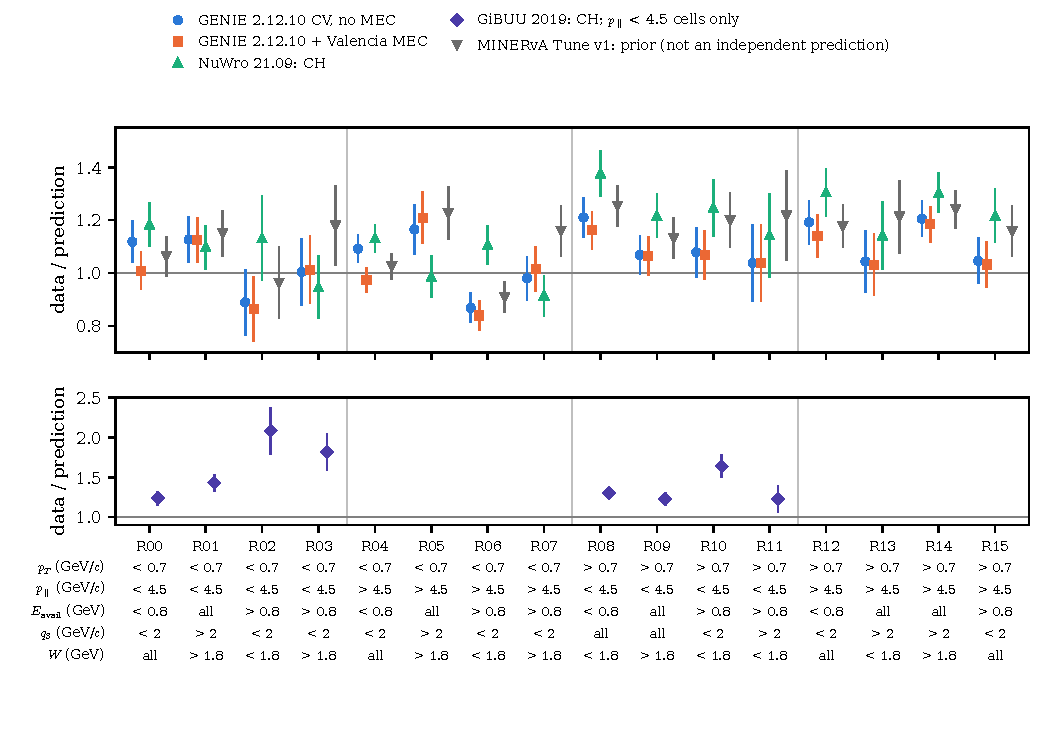
\includegraphics[width=\textwidth]{fd_g_fig_ratio}
\caption{Illustrative output (Sec.~\ref{supp:output}). Data over prediction, $f/g$, on the sixteen cells for the five predictions of Table~\ref{tab:gen16}, all in the analysis definitions, with NuWro and GiBUU corrected to CH. Each error bar is $(f/g)\,\sigma/f$, with $\sigma$ the square root of the diagonal of $C_{\mathrm{total}}+C_{\mathrm{resp}}+C_{\mathrm{PL,5D}}$, and the predictions' finite-sample uncertainties are not drawn. GiBUU (lower panel) is shown on its 8 cells with $\pPar<\fvval{h2-mid-pz}$~GeV/$c$ only. The key below the axes gives each cell's box. The $\chi^2$ of Table~\ref{tab:gen16} uses the full covariance, whose correlations the error bars do not show.}
\label{fig:ratio16}
\end{figure}

\subsection{The generator predictions}
\label{app:gendefs}
% Moved from the paper (methods-short-20261109): round 5's paper_body.tex:81 at bc8673186, verbatim; its evidence route is that line's source comment there.
The external predictions for CH are the untuned GENIE~2.12.10 without (``GENIE CV'') and with (``GENIE + MEC'') the Valencia 2p2h component~\cite{Nieves:2011pp}, which models meson-exchange currents (MEC). NuWro~21.09~\cite{Golan:2012wx} and GiBUU~2019~\cite{Buss:2011mx} are generated on carbon; in the sixteen-cell comparison of Sec.~\ref{sec:gen16} they are corrected to CH by adding each generator's own free-proton prediction with weight \fvval{g-ch-hweight} per nucleon. All predictions are per nucleon of their target (CH, or carbon for NuWro and GiBUU elsewhere); GENIE and NuWro are reweighted event by event to the analysis flux, and the GiBUU sample stops at $E_{\nu}\approx\SI{20}{GeV}$. In the sixteen-cell comparison the predictions use the analysis definitions: $W$ with the struck nucleon's mass, or an average nucleon mass where the generator records none, and the muon angle from the beam axis, with each event's beam-direction offset sampled from the analysis simulation. This changes no cell of any prediction by more than \fvval{gdef-dmax-bound} of the cell's uncertainty (at most \fvval{gdef-dmax}). Elsewhere the predictions compute $W$ with the neutron mass for every event and measure $\pT$ about their own neutrino axis. Hydrogen has no quasielastic, 2p2h, or coherent $\nu_{\mu}$ charged-current channel, so normalizing per nucleon does not remove the difference between the targets. In GENIE's own CH sample, the carbon-only cross section per nucleon exceeds that of CH by \SI{8.3}{\percent} for $W<\SI{1.1}{GeV}$. The comparisons of NuWro and GiBUU on carbon contain a target difference of this kind (Ref.~\cite{AnalysisNote2026}, Secs.~\ref*{N-sec:eavailw-axis} and~\ref*{N-sec:eavailw-generators}).



This section gives the joint-test estimator's sixteen-cell output on the data, its covariance and descriptive comparisons with generator predictions, for the reasons and with the limits of Sec.~\ref{supp:output}. The sixteen cells, with their boxes, cross sections and uncertainties, are in Table~\ref{tab:fived16-cells}, and the per-group uncertainties and the correlation matrix of the reported covariance in Tables~\ref{tab:fived16-groups} and~\ref{tab:fived16-corr}.

\subsection{Descriptive comparison with generator predictions}
\label{sec:gen16}
% FIVED16-BEGIN the generator comparison on the sixteen cells (DECISION-20261026-joseph-5d-generator-comparison-presentation.md option 1; DECISION-20261027-joseph-chi2-table-format.md). The p-value question is in the wording packet for Joseph.

\begin{table}[tb]
\caption{$\chi^2$ for each prediction in the indicated comparison region, against the reported covariance $C_{\mathrm{total}}+C_{\mathrm{resp}}+C_{\mathrm{PL,5D}}$ and against the covariance without $C_{\mathrm{PL,5D}}$, each plus $V_g$, where $V_g$ is the prediction's finite-sample (diagonal) covariance. Shape-only $\chi^2$ frees the normalization. All five predictions are in the analysis definitions, with NuWro and GiBUU corrected to CH (Sec.~\ref{app:gendefs}). The ndf of each block is given in its heading.}
\label{tab:gen16}
\centering\scriptsize
  \begin{tabular}{@{}lcccc@{}} \toprule
 & \multicolumn{2}{c}{reported covariance} & \multicolumn{2}{c}{without $C_{\mathrm{PL,5D}}$} \\ \cmidrule(lr){2-3}\cmidrule(l){4-5}
Prediction & $\chi^2$ & shape-only $\chi^2$ & $\chi^2$ & shape-only $\chi^2$ \\ \midrule
\multicolumn{5}{@{}l}{All 16 cells: ndf \fvval{g-gcv-total-ndf}, shape-only \fvval{g-gcv-shape_only-ndf}} \\
\fvval{label-gcv} & \fvval{g-gcv-total-chi2int} & \fvval{g-gcv-shape_only-chi2int} & \fvval{g-gcv-total-chi2int-nopl} & \fvval{g-gcv-shape_only-chi2int-nopl} \\
\fvval{label-gmec} & \fvval{g-gmec-total-chi2int} & \fvval{g-gmec-shape_only-chi2int} & \fvval{g-gmec-total-chi2int-nopl} & \fvval{g-gmec-shape_only-chi2int-nopl} \\
\fvval{label-nuwro}$^{a}$ & \fvval{g-nuwro-total-chi2int} & \fvval{g-nuwro-shape_only-chi2int} & \fvval{g-nuwro-total-chi2int-nopl} & \fvval{g-nuwro-shape_only-chi2int-nopl} \\
\fvval{label-tune} & \fvval{g-tune-total-chi2int} & \fvval{g-tune-shape_only-chi2int} & \fvval{g-tune-total-chi2int-nopl} & \fvval{g-tune-shape_only-chi2int-nopl} \\ \midrule
\multicolumn{5}{@{}l}{8-cell subset, $\pPar<\fvval{h2-mid-pz}$~GeV/$c$: ndf \fvval{g-gibuu-total-ndf}, shape-only \fvval{g-gibuu-shape_only-ndf}} \\
\fvval{label-gibuu}$^{b}$ & \fvval{g-gibuu-total-chi2int} & \fvval{g-gibuu-shape_only-chi2int} & \fvval{g-gibuu-total-chi2int-nopl} & \fvval{g-gibuu-shape_only-chi2int-nopl} \\ \bottomrule
\end{tabular}
\par\smallskip\raggedright\footnotesize $^{a}$In NuWro's free-proton sample, the supplement generated at neutrino energies of 50--100~GeV is flagged: the events lost to generator aborts there were not shown to be negligible (\nsec{sec:joint5d-ch}). $^{b}$Corrected to CH with GiBUU's own free-proton sample, which enters with weight \fvval{g-ch-hweight} per nucleon. That sample failed its sampling-closure check, and its deep-inelastic events, \fvval{g-gibuu-hlab-dis}\,\% of it, do not conserve energy (\nsec{sec:joint5d-ch}).
\end{table}
% - B0-sentence round (DECISION-20261106-joseph-b0-reconciliation-sentence.md): Table III is defined, verbatim, before Sec. V's heading, so that it floats before Limitation 1's page break and does not split the held sentence G1b:paper-g-20 in the rater copy

Table~\ref{tab:gen16} compares the sixteen-cell output with five predictions through a $\chi^2$ against the reported covariance plus each prediction's finite-sample (diagonal) covariance $V_g$, with a shape-only $\chi^2$ beside it. The comparison is descriptive: its $\chi^2$ values establish no exclusion of a generator, and they depend on the covariance (below). For GENIE + MEC and the Tune~v1, the shape-only $\chi^2$ is within one unit of the total, although Fig.~\ref{fig:ratio16} shows both predictions below the data in most cells: freeing the normalization lowers $\chi^2$ only by the residual's component along the result's own cell values in the metric of the reported covariance, and for these two predictions that component is small. GiBUU's sample stops at $E_\nu=\fvval{cmodel-gibuu-enu}$~GeV, so GiBUU is compared on the 8 cells with $\pPar<\fvval{h2-mid-pz}$~GeV/$c$ only. MINERvA Tune~v1 is the simulation's prior. On carbon, NuWro gives $\chi^2=\fvval{g-nuwro-carbon-total-chi2int}$ (shape-only \fvval{g-nuwro-carbon-shape_only-chi2int}) and GiBUU \fvval{g-gibuu-carbon-total-chi2int} (\fvval{g-gibuu-carbon-shape_only-chi2int}). For GiBUU, the effect of the CH correction on the total $\chi^2$ depends on whether $C_{\mathrm{model}}$'s shape ratios are from carbon or CH and on the hydrogen sample (\nsec{sec:fived16-gen-target}). A native CH generation of NuWro agrees with the combination within a tolerance fixed in advance ($\sum z^2=\fvval{gnat-gen-sumz2}$ for 16 cells, largest $|z|=\fvval{gnat-gen-zmax}$, in the generators' own definitions). The size of $C_{\mathrm{model}}$ is not calibrated; Table~\ref{tab:cmodel16} gives how the total $\chi^2$ changes with it.
% - PRD read 1, R2 (the director): verified from the Stage G readout fd/gencmp-e/rerun1/chain/chdefs/with/readout/fd_g_readout.json (a19009e0): genie_mec total 229.09, shape-only 229.00; mnvtune_v1 262.06, 261.88; both rows equal at the printed integers, not a transcription error. The drop from freeing the normalization (100 f f^T) is, by construction, the residual's component along f in C^-1's metric; local arithmetic on the committed operands (referee-presentation-20261104/prd-read-1/R2-CHECK.txt) reproduces both chi2 and gives GLS scales of -0.013 and -0.018 (+-0.04). g < f in 13 and 14 of 16 cells (g_over_f_minus_1). check_round.py asserts both claims.
% GENCMP round: carbon values, defs.json table_2x2 {nuwro,gibuu}.carbon.analysis_definitions.reported (129.98/112.93, 45.49/24.94); the rise, CH - carbon in the analysis definitions (47.78 - 45.49 = +2.29; shape-only 24.94 -> 22.19); the GENIE-hydrogen sensitivity, ch.json gibuu.CH_genie_hydrogen (44.19, never the primary) against ch.json gibuu.carbon (45.25), step A in the generators' definitions (FD-GENCMP-REPORT.md sec. 2.1); native NuWro, native.json generator_definitions.rule (sum z^2 17.87 < 32.0, max |z| 2.24 <= 3.5; the analysis route also agrees, 16.92 and 2.23), report sec. 2.4. C_model's generator samples: nd-unfolding/pv-ladder/config.json:58-65 (nuwro_cv_xsec5d_full.npz, gibuu_cv_xsec5d_fluxfix.npz), the frozen C12 products of FD-GENCMP-DECLARATION.md sec. 2 control A1; not measured (it needs the pscratch S1 assembly), noted for the director's GENCMP amendment. C_model's target, measured since (DECISION-20261102-joseph-cmodel-keep-carbon-state-effect.md items 2-4): FD-GENCMP-AMENDMENT-E-ADDENDUM-E2-REPORT.md sec. 3 and 5, values e2-* from e2.json and x_e2_sens.out.txt (pinned as e2 and e2sens in make_values_fived16.py); the pairing's share, 47.78 - 45.10 = 2.68, exceeds the 2.29 rise: with C_model on CH, GiBUU's CH total (45.10) is below carbon (45.49).

\begin{table}[tb]
\caption{Change of each prediction's total $\chi^2$ of Table~\ref{tab:gen16} when $C_{\mathrm{model}}$'s NuWro and GiBUU shape ratios are taken from CH instead of carbon, when $C_{\mathrm{model}}$ is doubled, and when it is removed (\nsec{sec:fived16-gen-target}).}
\label{tab:cmodel16}
\centering\scriptsize
\begin{tabular}{@{}lrrr@{}} \toprule
Prediction & ratios from CH & doubled & removed \\ \midrule
\fvval{label-gcv} & $\fvval{e2-with-gcv-total-dchr1}$ & $\fvval{e2-with-gcv-total-dx2r1}$ & $\fvval{e2-with-gcv-total-dx0r1}$ \\
\fvval{label-gmec} & $\fvval{e2-with-gmec-total-dchr1}$ & $\fvval{e2-with-gmec-total-dx2r1}$ & $\fvval{e2-with-gmec-total-dx0r1}$ \\
\fvval{label-nuwro} & $\fvval{e2-with-nuwro-total-dchr1}$ & $\fvval{e2-with-nuwro-total-dx2r1}$ & $\fvval{e2-with-nuwro-total-dx0r1}$ \\
\fvval{label-gibuu} & $\fvval{e2-with-gibuu-total-dchr1}$ & $\fvval{e2-with-gibuu-total-dx2r1}$ & $\fvval{e2-with-gibuu-total-dx0r1}$ \\ \bottomrule
\end{tabular}
\end{table}
% Revision round 1 (sonnet-2 minor 12, "use a small table"): the prose list of these twelve values became this table; the keys are those the prose printed (e2-with-*-total-dchr1, -dx2r1, -dx0r1; e2.json and x_e2_sens.out.txt, pinned in make_values_fived16.py), in the prose's order, GENIE CV, GENIE + MEC, NuWro, GiBUU.

With the run-period block, each total $\chi^2$ is lower by \fvval{pl-chi2fall-total-lo}--\fvval{pl-chi2fall-total-hi}\,\% of its value without it, and each shape-only $\chi^2$ by \fvval{pl-chi2fall-shape_only-lo}--\fvval{pl-chi2fall-shape_only-hi}\,\%.
% Targeted round (DECISION-20261103-joseph-retire-density-gate.md item 3; ledger targeted-round-paper-20261103/ledger.md): (a) Table III's GiBUU footnote: B3's name, and its post hoc premise check at <= g-gibuu-hlab-sigc sigma_c with sigma_c defined, print in the note, sec_joint.tex sec:joint5d-ch (:327) and sec_fived16.tex sec:fived16-gen-target (:388); the footnote keeps the failed check and the DIS share.
% 5B text round, J2(a) (DECISION-20261031-joseph-j1-j2-and-protections-split.md item 2): two column groups, both with V_g; Option B's blocks kept, ndf once per block (asserted equal across the 16-cell predictions by make_values_fived16.py); caption amended. The falls: values_fived16.tex pl-chi2fall-* (over Table IV's predictions; after the GENCMP round 3.6-29.3 % total and 7.4-40.4 % shape-only), the referee's correction (astra-consult-5b-presentation-20261031/answer.txt).

Weakening only the flux correlations by \fvval{sens-alpha-pct}\,\% lowers the $\chi^2$ of the 16-cell predictions by \fvval{sens-flux-fall-lo}--\fvval{sens-flux-fall-hi}\,\%, and the same change to the detector or lateral correlations by at most \fvval{sens-detlat-fall-max}\,\%; with the correlations of the interaction, flux, detector and lateral groups removed, every 16-cell prediction keeps $\chi^2\geq\fvval{sens-joint-chi2-min}$ for 16 degrees of freedom. Bootstrapping the \fvval{fb-universes} flux universes, with the flux variances kept, gives \fvval{fb-plo}th--\fvval{fb-phi}th percentile bands for each 16-cell $\chi^2$ with edges within \fvval{fb-edge-max}\,\% of the reported value and a median at most \fvval{fb-offset-relmax}\,\% above it (\nsec{sec:fived16-gen}). These dependences calibrate neither set of values, and no exclusion of a generator follows.
% Targeted round (DECISION-20261103-joseph-retire-density-gate.md item 3; ledger targeted-round-paper-20261103/ledger.md): (a) the bands: "not the sensitivity to incorrect correlations that the weakening probes" and "not intervals for the chi2 under the true correlations" print in the note, sec_fived16.tex sec:fived16-gen (:311).
% FIVED16-END

\section{Two per-cell validity rules}
\label{supp:validity}
% Moved from the paper (methods-short-20261109): round 5's paper_body.tex:274 at bc8673186, verbatim; its evidence route is that line's source comment there.
Two validity rules, labelled separately, classify each cell. The first applies per cell the thresholds of the usage recommendations of Ref.~\cite{ATLAS:2024jets}: at least 5000 effective simulated events, here those of the simulation's weights, a deviation from that definition; a data statistical uncertainty below \SI{15}{\percent}; and $|z|\leq2$ at each of the 12 graded truths under the reported covariance. The first two are met in every cell (the smallest effective number is 331\,614, in R07, and the largest statistical uncertainty \SI{0.368}{\percent}, in R05), so the rule rests on the third, and its recommended test of correlation assumptions on pseudo-data is not met here. Fourteen cells are valid under it; R02 and R06 fail, each from the GiBUU hybrid truth alone, at $z=+4.19$ and $+4.53$. The second rule is ours, not taken from Ref.~\cite{ATLAS:2024jets}: a cell is valid if the spread of its fake-data bias over the graded truths is less than half the spread of the generator predictions, $\rho<0.5$, in each of four noise treatments, which agree in every cell. Fourteen cells are valid under it; R08 ($\rho=0.522$--0.534) and R15 (0.564--0.565) are not, and the largest $\rho$ among the valid cells is 0.444, in R10. The threshold of 0.5 is our choice: at $1/3$, 11 cells are valid, and at 1, all 16. Twelve cells are valid under both rules. The two rules test different things, the first one truth's closure pull and the second the size of the bias spread relative to the generator spread, and neither validates an interval, since the fake-data tests grade bias, not coverage.


\printbibliography
\end{document}
